% !TEX TS-program = xelatex
% !TEX encoding = UTF-8

% This is a simple template for a XeLaTeX document using the "article" class,
% with the fontspec package to easily select fonts.

%\documentclass[oneside,10pt]{article} % use larger type; default would be 10pt
\documentclass[oneside,10pt]{book}
% other LaTeX packages.....

%-------------------------------------------------
% Geometry (et sidenotes) : format tufte light
%-------------------------------------------------

\usepackage{sidenotes}

%\usepackage{mwe}

%\usepackage[showframe]{geometry}
\usepackage{geometry}

% option classique
\geometry{letterpaper, left=2cm, right=3in, top=50pt,bottom=50pt, marginparsep=20pt, marginparwidth=2in,  footskip=40pt}

% Option pour faire un document A5
%\geometry{paperwidth=6in, paperheight=9in, left=2cm, right=2in, top=50pt,bottom=50pt, marginparsep=20pt, marginparwidth=1.5in,  footskip=40pt}
 
\renewcommand{\baselinestretch}{1.1} 
\usepackage{placeins} % floatbarrier
\usepackage{fullwidth}
 
\makeatletter
%\renewcommand{\@sidenotes@adjust}{%
% \checkoddpage%
% \ifoddpage%
% %
% \else%
% %\hspace{\@sidenotes@extrawidth}%    %% this was originally there
% \fi}
%%
%% or
%%
\let\@sidenotes@adjust\relax
\makeatother

\setlength\parindent{0pt}
%\usepackage{marginnote}
%\renewcommand*{\raggedleftmarginnote}{}
%\renewcommand*{\raggedrightmarginnote}{}

% Margin Caption (done with sidenotes package)
% UTILISER \sidecaption pour une caption
%\usepackage[margincaption,rightcaption,ragged,wide]{sidecap}
%\usepackage[margincaption,outercaption]{sidecap}
%\sidecaptionvpos{figure}{t} 
%\sidecaptionvpos{table}{t}
% format des captions des figures
%\captionsetup[SCfigure]{format=plain, ...}
%\captionsetup[SCtable]{format=plain, ...}
%-------------------------------------------------
% cadre
%-------------------------------------------------

\usepackage{tikz}
\usepackage[framemethod=TikZ]{mdframed}
\usetikzlibrary{positioning}  
\usepackage{placeins} % FLoatbarrier to force float

\usepackage{xcolor}
%\hypersetup{colorlinks}% uncomment this line if you prefer colored hyperlinks (e.g., for onscreen viewing)
\usepackage{units}
% Typesets the font size, leading, and measure in the form of 10/12x26 pc.


\newcommand{\measure}[3]{#1/#2$\times$\unit[#3]{pc}}
\newcommand{\coefGraph}{1} % Taille du graphe dans les marges; sert uniquement pour Epub, sinon = 1 x textwidth
%\usepackage{multicol} %multicolum for Definition
\newcommand{\largecoefGraph}{1.2} % Taille du graphe dans les marges en proportion de textwidth; sert uniquement pour Epub, sinon = textwidth; remplacer \textwidth par \coefGraph\textwidth
%\usepackage[table]{xcolor}
%\usepackage[xcdraw]{xcolor}
%\usepackage[dvipsnames]{xcolor}
%\usepackage{amsmath,amssymb,amsthm}
%\usepackage{mathtools}
%\usepackage{mathspec}
%\usepackage{xltxtra,xunicode}
\newcommand{\myinnertopmargin}{0pt} % marge qui sert pour les définitions et proprietés




%-------------------------------------------------
% url
%-------------------------------------------------

\usepackage{blindtext}
\usepackage{hyperref}
\usepackage{url}


%-------------------------------------------------
% tableau
%-------------------------------------------------

% pour mettre des tableaux au bon endroit avec l'option H
%\usepackage{float}
% grands tableaux... pratiques
\usepackage{longtable}
 % pour faire des beaux tableaux
\usepackage{booktabs}

 
%-------------------------------------------------
% caractère
%-------------------------------------------------




\usepackage[sc]{mathpazo}
\linespread{1.05}         % Palladio needs more leading (space between lines)

\usepackage{fontspec} % Font selection for XeLaTeX; see fontspec.pdf for documentation
\defaultfontfeatures{Mapping=tex-text} % to support TeX conventions like ``---''


%\setmainfont{Charis SIL} % set the main body font (\textrm), assumes Charis SIL is installed
%\setsansfont{Deja Vu Sans}
%\setmonofont{Deja Vu Mono}

 % format des fonts comme Tufte
 \usepackage{xunicode} % Unicode support for LaTeX character names (accents, European chars, etc)
\usepackage{xltxtra} % Extra customizations for XeLaTeX
\usepackage{amsmath}
\usepackage{amsthm}
% \usepackage{fontspec}
%\setmainfont[Renderer=Basic, Numbers=OldStyle, Scale = 1.0]{TeX Gyre Pagella}
%\setsansfont[Renderer=Basic, Scale=0.90]{TeX Gyre Heros}
%\setmonofont[Renderer=Basic]{TeX Gyre Cursor}
% Palatino for main text and math
%\usepackage[osf,sc]{mathpazo}

% Helvetica for sans serif
% (scaled to match size of Palatino)
%\usepackage[scaled=0.90]{helvet}

% Bera Mono for monospaced
% (scaled to match size of Palatino)
%\usepackage[scaled=0.85]{beramono}
 
%\setmainfont[Numbers=OldStyle, Scale = 1.0]{TeX Gyre Pagella}
%\setsansfont[Scale=0.90]{TeX Gyre Heros}
%\setmonofont{TeX Gyre Cursor}

% pour le chinois
\usepackage{xeCJK}

%-------------------------------------------------
% caractère
%-------------------------------------------------

%\usepackage{biblatex} %pour citer des numero de page
\usepackage[utf8x]{inputenc}

\usepackage[english,main=french]{babel}



\babelprovide[import]{arabic}
\babelfont[arabic]{rm}{Amiri}
\babelprovide[import]{greek}
\babelfont[greek]{rm}{EB Garamond}
% ex
% \foreignlanguage{greek}{Ἰουδαῖοί τε καὶ προσήλυτο.}
%\babelprovide[import]{greek}
%\babelfont[greek]{rm}[RawFeature=+calt]{SimonciniGaramondPro}
\usepackage{arabtex}
%babel-greek
%\usepackage[sc]{mathpazo}

%\linespread{1.05}         % Palladio needs more leading (space between lines)
%\usepackage[T1]{fontenc}
%\renewcommand{\cftsecfont}{\rmfamily\mdseries\upshape}
%\renewcommand{\cftsecpagefont}{\rmfamily\mdseries\upshape} % No bold!

%TARabe dans Name


%Recherche \hypertarget et remplacer par \vide
% \protect\hyperlink par \vide
%\texorpdfstring par RIEN
% \RL : \TArabe
% rechercher \footnote{ et remplacer par \sn{
% rechercher Al Gazali
% package pour faire des réferences à des labels pour le chapitre théologiens
 
%-------------------------------------------------
% bibliography
%-------------------------------------------------

% 
%\usepackage{natbib}
\usepackage{natbib}
\bibliographystyle{unsrtnat}
\bibliographystyle{kluwer}
%\usepackage[notes,backend=biber]{biblatex-chicago}

%\usepackage[style=reading]{biblatex}
%\usepackage[citestyle=reading,bibstyle=authortitle]{biblatex}

%\addbibresource{Theo.bib}

%\bibliography{sample}
%\bibliography{siam}

%\newcommand*{\sidecite}[1]{\sidenote{[\cite{#1}].\citeauthor{#1} - \citetitle{#1}}



 %--------------------------------------------------------------
% Table des matières
%--------------------------------------------------------------
 \usepackage{titletoc}
%%%%% TABLE OF CONTENTS
\setcounter{tocdepth}{1}

\usepackage{etoc}
%%% ToC (table of contents) APPEARANCE
%\usepackage[nottoc,notlof,notlot]{tocbibind} % Put the bibliography in the ToC
%\usepackage[titles,subfigure]{tocloft} % Alter the style of the Table of Contents

\usepackage{cleveref} % referece



\usepackage{eurosym}  %Euro
\usepackage[super]{nth} %for \nth{1} to give 1st
\usepackage{array} % permet de centrer les tableaux\

% Prints the month name (e.g., January) and the year (e.g., 2008)




%\splittopskip=5cm 

 
%-------------------------------------------------
% édition
%-------------------------------------------------
\usepackage{comment}

%-------------------------------------------------
% multi colonnage
%-------------------------------------------------
\usepackage{multicol}





%--------------------------------------------------------------
% Frame
%--------------------------------------------------------------

\usepackage[framemethod=TikZ]{mdframed}

\usepackage{thmtools}
%\usepackage{amsthm}

\usepackage{blindtext} % avoid to cut theorem
% avoid to have theorem or definition in the list of theorm
\makeatletter
\newcommand{\theosep}{\parsep}
\renewcommand{\theosep}{20pt}


%--------------------------------------------------------------
% Titre des listes de théorèmes
%--------------------------------------------------------------

\renewcommand{\listtheoremname}{List of Important Theorems}

\makeatletter
\def\ll@theorem{%
  \protect\numberline{\csname the\thmt@envname\endcsname}%
  \ifx\@empty\thmt@shortoptarg
    \thmt@thmname
  \else
    \thmt@shortoptarg
  \fi}
\def\l@thmt@theorem{} 
 \makeatother
 

% avoid to have theorem or definition in the list of theorm
\makeatletter
\patchcmd\thmt@mklistcmd
  {\thmt@thmname}
  {\check@optarg{\thmt@thmname}}
  {}{}
\patchcmd\thmt@mklistcmd
  {\thmt@thmname\ifx}
  {\check@optarg{\thmt@thmname}\ifx}
  {}{}
\protected\def\check@optarg#1{%
  \@ifnextchar\thmtformatoptarg\@secondoftwo{#1}%
}

 
\makeatother

% format of theorem


            
\declaretheoremstyle[
    headfont=\scshape, 
    notebraces={\scshape : }{.},
    bodyfont=\normalfont,
    headpunct={},
    postheadspace=\newline,
%    postheadhook={\textcolor{red}{\rule[.6ex]{\linewidth}{0.4pt}}\\},
    spacebelow=\parsep,
    spaceabove=\parsep,
    mdframed={
            backgroundcolor=white!20, 
            splittopskip = \topskip,
            linecolor=blue!30, 
            linewidth = 2pt,
            innertopmargin=\myinnertopmargin,
            roundcorner=1pt, 
            innerbottommargin=6pt, 
            skipabove=\parsep,     
            skipbelow=\parsep} 
    ]{Definitionstyle}
    
\declaretheoremstyle[
    headfont=\scshape, 
    notebraces={\scshape : }{.},
    bodyfont=\normalfont,
    headpunct={},
    postheadspace=\newline,
%    postheadhook={\textcolor{red}{\rule[.6ex]{\linewidth}{0.4pt}}\\},
    spacebelow=\parsep,
    spaceabove=\parsep,
    mdframed={backgroundcolor=white!20, 
            splittopskip = \topskip,
            linecolor=red!30, 
            linewidth = 2pt,
            innertopmargin=\myinnertopmargin,
            roundcorner=1pt, 
            innerbottommargin=6pt, 
            skipabove=\parsep,     
            skipbelow=\parsep} 
    ]{Propertystyle}

%,    postfoothook=
% example environment - thmtools
\declaretheoremstyle[
    headfont=\scshape, 
    notebraces={\scshape : }{.},
    bodyfont=\normalfont,
    headpunct={},
    postheadspace=\newline, 
%    postheadhook={\textcolor{red}{\rule[.6ex]{\linewidth}{0.4pt}}\\},
    spacebelow=\parsep,
    spaceabove=\parsep
]{Exercisestyle}
% example environment - thmtools








\declaretheorem[ style = Exercisestyle, numbered=no,name = Property]{property}
\declaretheorem[ style = Propertystyle, name = {Property} ]{Prop}
\declaretheorem[ style = Propertystyle, name = Theorem, sibling=Prop]{Theo}
\declaretheorem[ style = Propertystyle, name = Theorem, sibling=Prop]{theorem}
\declaretheorem[ style = Propertystyle, name = Lemma, sibling=Prop]{lemma}
\declaretheorem[ style = Exercisestyle, numbered=no,name = {Remark}]{rem}
\declaretheorem[ style = Definitionstyle, name = {Definition}]{definition}
\declaretheorem[ style = Definitionstyle, name = {Definition}, sibling=definition]{Def}
\declaretheorem[ style = Exercisestyle, name = Exercise]{exercise}
\declaretheorem[ style = Exercisestyle, name = Exercise, sibling=exercise]{Exercise}
\declaretheorem[ style = Exercisestyle, name = Exercise, sibling=exercise]{Exc}
\declaretheorem[ style = Exercisestyle, name = Exercise, sibling=exercise]{Exo}
\declaretheorem[ style = Exercisestyle, name = Problem, sibling=exercise]{problem}
\declaretheorem[ style = Exercisestyle, name = Example]{example}
\declaretheorem[ style = Exercisestyle, name = Example, sibling=example]{Ex}
\makeatother


%--------------------------------------------------------------
% Code
%--------------------------------------------------------------

%% Permet de mettre du code
\usepackage{listings}
\lstdefinestyle{mystyle}{
    basicstyle=\ttfamily\footnotesize,
    breakatwhitespace=false,         
    breaklines=true,                 
    captionpos=b,                    
    keepspaces=true,                 
    numbers=left,                    
    numbersep=5pt,                  
    showspaces=false,                
    showstringspaces=false,
    showtabs=false,                  
    tabsize=2
}
\lstset{%
	aboveskip=\topsep,
	belowskip=\topsep,
	xleftmargin=\parindent}

\lstset{style=mystyle}





\newcommand{\bi}{\begin{itemize}}
 \newcommand{\ei}{\end{itemize}}
  \newcommand{\be}{\begin{Ex}}
 \newcommand{\ee}{\end{Ex}}
 \newcommand{\mn}[1]{\marginnote{\footnotesize #1}}
  \newcommand{\sn}[1]{\sidenote{\footnotesize #1}}

\newcommand{\mzt}{\emph{muʿtazilite}}  
\newcommand{\CD}{\emph{la Cité de Dieu }}  

\newcommand{\CB}{\emph{Cedric Baylocq }} % nom du professeur
%Recherche \hypertarget et remplacer par \vide
% \protect\hyperlink par \vide
%\texorpdfstring par RIEN
% \RL : \TArabe
% rechercher \footnote{ et remplacer par \sn{
% rechercher Al Gazali
%\newcommand\TArabe[1]{\foreignlanguage{arabic}{\RL}}
\newcommand\TArabe[1]{\foreignlanguage{arabic}{#1}}
\newcommand{\vide}[1]{}

\renewcommand{\listtheoremname}{Liste des Definitions}

% Prints the month name (e.g., January) and the year (e.g., 2008)
\newcommand{\monthyear}{%
  \ifcase\month\or January\or February\or March\or April\or May\or June\or
  July\or August\or September\or October\or November\or
  December\fi\space\number\year
}

\newcommand{\tnote}{\textsuperscript}


% Inserts a blank page
\newcommand{\blankpage}{\newpage\hbox{}\thispagestyle{empty}\newpage}


% Prints an epigraph and speaker in sans serif, all-caps type.
\newcommand{\openepigraph}[2]{%
  %\sffamily\fontsize{14}{16}\selectfont
  \begin{fullwidth}
  \sffamily\large
  \begin{doublespace}
  \noindent\allcaps{#1}\\% epigraph
  \noindent\allcaps{#2}% author
  \end{doublespace}
  \end{fullwidth}
}
 


 

% Prints argument within hanging parentheses (i.e., parentheses that take
% up no horizontal space).  Useful in tabular environments.
\newcommand{\hangp}[1]{\makebox[0pt][r]{(}#1\makebox[0pt][l]{)}}
\newcommand{\hangstar}{\makebox[0pt][l]{*}}
%%
% Prints an asterisk that takes up no horizontal space.
% Useful in tabular environments.



% Macros for typesetting the documentation
\newcommand{\hlred}[1]{\textcolor{Maroon}{#1}}% prints in red
\newcommand{\hangleft}[1]{\makebox[0pt][r]{#1}}
\newcommand{\hairsp}{\hspace{1pt}}% hair space
\newcommand{\hquad}{\hskip0.5em\relax}% half quad space

\newcommand{\ie}{\textit{i.\hairsp{}e.}\xspace}
\newcommand{\eg}{\textit{e.\hairsp{}g.}\xspace}
\newcommand{\na}{\quad--}% used in tables for N/A cells

% Prints an epigraph and speaker in sans serif, all-caps type.





%%
\usepackage{graphicx} % support the \includegraphics command and options


%\date{} % Activate to display a given date or no date (if empty),
         % otherwise the current date is printed 

\begin{document}
 
%\citestyle{verbose}




%-------------------------------------



\pagenumbering{arabic} 
\setcounter{page}{1}
 



%\chapter{Les religions comme des cultures }

\mn{le 9/5/22}

\section{Bibliographie}
CHENO, R., Dieu au pluriel. Penser les religions, Cerf, Paris, 2017. 

CDF, Dominus Iesus, 2000. 

CTI, Le christianisme et les religions, 1997 

DUBUISSON, D., L’invention des religions, Paris, CNRS éditions, 2020. 

DUPUIS, J. Vers une théologie chrétienne du pluralisme religieux, Cerf, Paris, 1997. 

DURAND, M-L., « Le rapport Église/peuple juif comme paradigme du rapport aux autres religions et quasi-religions séculières ? » dans E. PISANI (dir.), Maximum illud. Aux sources d’une nouvelle ère missionnaire, Paris, Cerf, 2020, p. 141-152. 

DURKHEIM, E., Les formes élémentaires de la vie religieuse, PUF, Paris, 20086. 

ELIADE, M., Aspects du mythe, Gallimard, Paris, 1963. 

FEDOU, M., Les religions selon la foi chrétienne, Paris, Cerf, 1996. 

GUÉ, X., « Comment la théologie postlibérale pense-t-elle l’universalité des vérités religieuses ? Une relecture de La nature des doctrines de G. Lindbeck » dans E. PISANI (dir.), Les doctrines religieuses sont-elles condamnées à s’opposer ? Actes du colloque de l’ISTR des 6 et 7 février 2020, Paris, Cerf, 2021, 25-51. 

JEAN-PAUL II, Lettre encyclique Redemptoris missio, 1990. 

LINDBECK, G. A., La nature des doctrines. Religion et théologie à l’âge du postlibéralisme, tr. de M. HEBERT, Paris, Van Dieren éditeur, 2002. 

PHILIPS, l’Église et son mystère au IIe concile du Vatican, t. 1, Desclée, Paris 1967 

SALENSON, C., « La Missio Dei » dans E. PISANI (dir.), Maximum illud. Aux sources d’une nouvelle ère missionnaire, Paris, Cerf, 2020, p. 125-140. 

VILLEMIN, L. et CHEVALLIER, G. , « La distinction « incorporé à / ordonné à » dans Lumen Gentium : quelles conséquences pour la compréhension du rapport Eglise / Royaume ? », in Christoph THEOBALD (dir.), Pourquoi l’Eglise ? La dimension ecclésiale de la foi dans l’horizon du salut, Paris : Bayard, 2014, pp. 165-196. 

WILLAIME, J-P., Sociologie des religions, PUF, Paris, 20125. 



\section{Introduction}
\paragraph{la religion comme socialisation} en répondant aux grandes questions

\begin{quote}

À notre époque où le genre humain devient de jour en jour plus étroitement uni et où les relations entre les divers peuples se multiplient, l’Église examine plus attentivement quelles sont ses relations avec les religions non chrétiennes. Dans sa tâche de promouvoir l’unité et la charité entre les hommes, et aussi entre les peuples, elle examine ici d’abord ce que les hommes ont en commun et qui les pousse à vivre ensemble leur destinée.

Tous les peuples forment, en effet, une seule communauté ; ils ont une seule origine, puisque Dieu a fait habiter tout le genre humain sur toute la face de la terre [1] ; ils ont aussi une seule fin dernière, Dieu, dont la providence, les témoignages de bonté et les desseins de salut s’étendent à tous [2], jusqu’à ce que les élus soient réunis dans la Cité sainte, que la gloire de Dieu illuminera et où tous les peuples marcheront à sa lumière [3].

Les hommes attendent des diverses religions la réponse aux énigmes cachées de la condition humaine, qui, hier comme aujourd’hui, agitent profondément le cœur humain : Qu’est-ce que l’homme? Quel est le sens et le but de la vie? Qu’est-ce que le bien et qu’est-ce que le péché? Quels sont l’origine et le but de la souffrance? Quelle est la voie pour parvenir au vrai bonheur? Qu’est-ce que la mort, le jugement et la rétribution après la mort ? Qu’est-ce enfin que le mystère dernier et ineffable qui embrasse notre existence, d’où nous tirons notre origine et vers lequel nous tendons ?
    Nostra aetate 1
\end{quote}

\subsection{Mircea Eliade et la spécificité du phénomène religieux }

\paragraph{Le phénomène religieux }

\begin{quote}
    « Le mythe raconte une histoire sacrée ; il relate un événement qui a eu lieu dans le temps primordial, le temps fabuleux des ‘commencements’. Autrement dit, le mythe raconte comment, grâce aux exploits des Etres Surnaturels, une réalité est venue à l’existence (…). C’est donc toujours le récit d’une ‘création’ : on rapporte comment quelque chose a été produit, a commencé à être. Le mythe ne parle que de ce qui est arrivé réellement, de ce qui s’est pleinement manifesté (…). En somme, les mythes décrivent les diverses, et parfois dramatiques, irruptions du sacré (ou du ‘sur-naturel’) dans le Monde. C’est cette irruption du sacré qui fonde réellement le Monde et qui le fait tel qu’il est aujourd’hui. Plus encore : c’est à la suite des interventions des Etres Surnaturels que l’homme est ce qu’il est aujourd’hui, un être mortel, sexué et culturel » (Eliade, Aspects du mythe, 16-17). 
\end{quote}

\paragraph{Le mythe à l’origine de la culture et de la société }

\begin{quote}
    « Du fait que le mythe relate les gesta des Etres Surnaturels et la manifestation de leurs puissances sacrées, il devient le modèle exemplaire de toutes les activités humaines significatives » (Eliade, Aspects, 17-18).  
\end{quote}

\begin{quote}
    « Pour l’homme des sociétés archaïques (…) ce qui s’est passé ab origine est susceptible de se répéter par la force des rites. L’essentiel est donc, pour lui, de connaître les mythes. Non seulement parce que les mythes lui offrent une explication du Monde et de son propre mode d’exister dans le Monde, mais surtout parce que, en se les remémorant, en les réactualisant, il est capable de répéter ce que les Dieux, les Héros ou les Ancêtres ont fait a l'origine. Connaître les mythes, c’est apprendre le secret de l’origine des choses. En d’autres termes, on apprend non seulement comment les choses sont venues à l’existence, mais aussi où les trouver et comment les faire réapparaître lorsqu’elles disparaissent » (Eliade, Aspects, 26). 
\end{quote}

\subsection{Durkheim et la « sociogenèse » de la religion }

Thèse sur le totem en Australie, \textit{idéalisation de la société}. 
Les formes élémentaires de la religion

\paragraph{Distinction entre profane et le sacré} On se comporte différemment. La religion génère du sacré : 
\begin{quote}
    « Toutes les croyances religieuses connues (….) supposent une classification  des choses (…) que se représentent les hommes, en deux classes, en deux genres opposés (…) le profane et le sacré. (…) Les croyances, les mythes (…) sont ou des représentations ou des systèmes de représentations qui expriment la nature des choses sacrées, les vertus et les pouvoirs qui leur sont attribués, leur histoire, leurs rapports les unes avec les autres et avec les choses profanes » (Durkheim, 50-51).  
\end{quote}

Ce sont les hommes qui ont séparés ces deux mondes. Le monde séparé entre profane et religieux.

\paragraph{Définition de la religion}
\begin{quote}
« Une religion\sn{Durkheim, Les formes élémentaires
de la vie religieuse, 65} est un système solidaire de croyances et de pratiques relatives à des choses sacrées, c’est-à-dire séparées, inter-
dites, croyances et pratiques qui unissent en une même communauté
morale, appelée Église, tous ceux qui y adhèrent »
\end{quote}

\paragraph{Distinction entre Religion et Magie}
La magie ne fait pas \textit{corps}, \textit{Eglise}. Les clients d'un magicien peuvent n'avoir aucun lien entre eux. 
\begin{quote}
    « Les croyances proprement religieuses sont toujours communes à une collectivité déterminée qui fait profession d’y adhérer et de pratiquer les rites qui en sont solidaires. (…) \textbf{(Les croyances) sont la chose du groupe et elles en font l’unité.} Les  individus qui composent (la collectivité) se sentent liés les uns aux autres, par cela seul qu’ils ont une foi commune. Une société dont les membres sont unis parce qu’ils se représentent de la même manière le monde sacré et ses rapports avec le monde profane, et parce qu’ils traduisent cette représentation commune dans des pratiques identiques, c’est ce qu’on appelle une Église » (Durkheim, 60). 
\end{quote}

La religion génère les groupements, elle est par nature collective.


\paragraph{la société est la source de la religion} Pourquoi ont ils fait la distinction entre profane et sacré ? Alors que le sensible ne permet pas de faire cette distinction ?

\begin{quote}
    « Nous avons montré quelles forces morales (la société) développe et comment elle éveille ce sentiment d’appui, de sauvegarde, de dépendance tutélaire qui attache le fidèle à son culte. C’est elle qui l’élève au-dessus de lui-même : c’est même elle qui le fait. Car ce qui fait l’homme, c’est cet ensemble de bien intellectuels qui constitue la civilisation, et la civilisation est l’œuvre de la société.[…] Pour que les principaux aspects de la vie collective aient commencé par n’être que des aspects variés de la vie religieuse, il faut évidemment que la vie religieuse soit la forme éminente et comme une expression raccourcie de la vie collective tout entière. \textsc{Si la religion a engendré tout ce qu’il y a d’essentiel dans la société, c’est que l’idée de la société est l’âme de la religion} » (Durkheim, 598-599). 
\end{quote}

\begin{Synthesis}
la société élève l'homme, qui permet de se dépasser. 
\end{Synthesis}



\begin{quote}
    « Pour que la société puisse prendre conscience de soi et entretenir, au degré d’intensité nécessaire, le sentiment qu’elle a d’elle-même, il faut qu’elle s’assemble et se concentre. Or, cette concentration détermine une exaltation de la vie morale qui se traduit par un ensemble de conceptions idéales où vient se peindre la vie nouvelle qui s’est ainsi éveillé (…) Une société ne peut ni se créer ni se recréer sans, du même coup, créer l’idéal. (…) La société idéale n’est pas en dehors de la société réelle ; elle en fait partie. (…)\textsc{ Car une société n’est pas simplement constituée par la masse des individus qui la composent (…) mais, avant tout, par l’idée qu’elle se fait d’elle-même.} »(Durkheim, 603-604). 
\end{quote}

\begin{Def}[Religion]
On va sacraliser la société, une hypostase qui a une conscience.  Appartenir à cette société hypostasiée. Elle génère la religion. 
\end{Def}

Et comment fait on dans une société pluraliste ?
\begin{Ex}
Lors de la séparation de l'Eglise et de l'Etat, la société a essayé de singer la religion, avec l'instituteur comme \textit{prêtre}.
\end{Ex}

\paragraph{La religion comme un facteur de cohésion et une force sociale } Force sociale pour supporter les épreuves.
\begin{quote}
    « Le fidèle qui a communié avec son dieu n’est pas seulement un homme qui voit des vérités nouvelles que l’incroyant ignore ; c’est un homme qui peut davantage. Il sent en lui plus de force soit pour supporter les difficultés de l’existence, soit pour les vaincre » (Durkheim, 595).  
\end{quote}

\paragraph{Critique de la théorie sociologique de Durkheim } Première critique, Dieu n'est pas pris en charge dans la religion. Dieu serait une projection de la société. Feuerbach : 
\begin{quote}
    projection d'une... divinisé
\end{quote}

Par ailleurs, la religion est une instance critique de la société. On ne peut pas la réduire à une simple projection idéale de la société. Et comment on fait en cas de société pluri-confessionnelle ?


\begin{quote}
    « Les hommes vivent sur la même planète, mais dans des mondes différents. Chaque culture (…) conçoit en effet le monde à sa manière » (Dubuisson, 211). 
\end{quote}

\begin{quote}
    « Toutes les cultures, toutes les sociétés ont conçu le monde, l’univers à leur manière. Et (…) toujours en ont imaginé la genèse dans un mythe ou une série de mythes cosmogoniques. Chacune de ces conceptions est différente des autres, mais toutes se ressemblent en ce sens où chaque culture vit (…) dans son propre monde et que ces mondes remplissent partout les mêmes fonctions » (Dubuisson, 212). 
\end{quote}

La langue est toujours dans une culture, et la religion est aussi insérée.

\section{L’approche théologique post-libérale des religions }

\subsection{La critique de l’idée d’une essence commune à toutes les religions}
\paragraph{La remise en cause question d’un « lieu tiers } jusqu'à présent, on a essayé de trouver un PPDC : expérience spirituelle,...

\begin{quote}
    « Il suffirait, selon les pluralistes, de débarrasser chaque religion de son appareil dogmatique et symbolique propre pour retrouver ce lieu tiers, cet arrière-plan commun. Le théologien pluraliste, c’est celui qui sait dépasser sa propre tradition pour s’enraciner dans ce lieu tiers d’où il observe toutes les religions et contemple leur convergence » (Chéno, 111-112). 
\end{quote}

Il s'agit de changer cette approche et de se remettre au sein de notre identité, dans notre religion.
De plus, cette mise en aplomb, trouvant un terrain commun, est une version occidentale, mais qui ne respecte pas forcément l'autre.


\paragraph{Le tournant opéré par G. Lindbeck  } Un des initiateurs du \textit{post-libéralisme}, contre le libéralisme (protestant). Le courant libéral dans le catholicisme était attenué par la force du magistère.
Lindbeck a travaillé au concile.  En 1984, il publie la \textit{nature des doctrines}. \textit{Comment on conçoit la vérité en Christianisme ?}

 
 \begin{quote}
     « On considère (…) les religions comme des idiomes différents permettant d’interpréter la réalité, d’exprimer l’expérience et d’organiser la vie (…) Ainsi, les questions qui se posent quand on compare les religions concernent tout d’abord l’adéquation de leurs catégories » (Lindbeck p. 55). 
 \end{quote}
 Mon voisin fait une expérience ineffable mais va le dire de façon différente. Quelle est la vérité noumenale ? Efficacité de leur symbole : mesurera la qualité de la répone. 
  \paragraph{Approche culturo linguisitique}
 

  Le religions sont comme des archipels.
 
 \subsection{Les religions sont incommensurables quant à leur contenu}



 
 \paragraph{Dialoguer entre religion est il pertinent ? }
 
  \begin{quote}
     Qu’une religion soit raisonnable [donc universelle] dépend largement de ses pouvoirs d’assimilation, de sa capacité à fournir dans ses propres termes une interprétation intelligible des diverses situations et réalités que rencontrent ses adhérents. Les religions que nous qualifions de primitives échouent régulièrement à ce test quand elles sont confrontées à des changements importants, tandis que les religions mondiales développent de plus grandes ressources pour faire face aux vicissitudes (Lindbeck, 175). 
 \end{quote}
 
 Toute religion est comme une langue et donc universelle.
 
  \subsection{Les religions sont comparables quant à leur fonction}
  
  Lindbeck ne se met dans une confession particulière : ni chrétienne, ni théologique, mais scientifique et sociologique. Décentrement. 
  Il les définit comme : 
  
   \begin{quote}
     « Les religions […] ressemblent à des langues, ce qui les assimile à des cultures (dans la mesure où ces cultures sont comprises de manière sémiotique comme des systèmes de réalités et de valeurs, c’est-à-dire comme des idiomes qui permettent de construire la réalité et de vivre au quotidien). »  (Lindbeck, p. 16). 
 \end{quote}
  
  \begin{Def}[religion pour Lindbeck]
  Les religions […] ressemblent à des langues.
  \end{Def}
  
  Des mythes, des récits (ex : Gn 1 permet de comprendre le monde, moi-même). Par exemple, pour dire une conversion, on va reprendre le schéma de Charles de Foucauld ou Paul. Jamais pure innovation.
  \paragraph{Image des lunettes} Les religions sont des lunettes à travers lesquelles on voit le monde. 
  
  Ce n'est pas l'idée qui précède le langage, c'est le langage qui nous précède et nous utilisons le langage qui nous est disponible. 
  
  \paragraph{Fécondité performatrice des religions}
  En se référant à Luther, la vérité se vit parce qu'elle est reçue qui y adhère. 
  
  

\begin{quote}
    dire la vérité religieuse \ldots c'est s'engager dans un style de vie.
\end{quote}
 Pas une définition théorique de la vérité, mais une vérité pratique.
  
  \subparagraph{Performatrice} \textit{Je promets de te rester fidèle}. 
  
  \subparagraph{Pour découvrir la tradition de l'autre, rencontrer quelqu'un qui essaye de conformer sa vie à sa tradition} Sinon, on risque d'avoir une mauvaise vision de l'autre.
  
  
  
  Si la religion permet de se comprendre, pourquoi il n'y aurait pas des religions plus universelles que d'autres ? Si on voit que certains sont heureux, il y a une dimension universelle ? Un aspect qui dépasse l'individu, qui serait \textsc{partageable}.
  
  \subparagraph{image de la langue} certaines langues nous ouvrent au monde, qui nous permette d'accueillir de nouvelles experiences du monde, et d'autres moins universelles que d'autres. C'est Lindberg qui dit cela, après avoir dit l'individualité.
  
  \begin{quote}
      Qu’une religion soit raisonnable [donc universelle] dépend largement de ses pouvoirs d’assimilation, de sa capacité à fournir dans ses propres termes une interprétation intelligible des diverses situations et réalités que rencontrent ses adhérents. Les religions que nous qualifions de primitives échouent régulièrement à ce test quand elles sont confrontées à des changements importants, tandis que les religions mondiales développent de plus grandes ressources pour faire face aux vicissitudes (Lindbeck, 175)
  \end{quote}
  
La vérité des religions est testée dans l'histoire. Il y a des traditions religieuses qui ont disparu. On verra à la fin de l'histoire, de façon eschatologique, la vérité des religions du jour. Si cela dure, il y a quelque chose de solide. 

  \paragraph{Fécondité sociale et universalité} 
  
  un autre aspect de la fécondité envisagé par Lindbeck, c'est la fécondité sociale.  Il réaffirme que la religion socialise les hommes, 
  
  \subparagraph{contraste avec l'approche libérale,} où des milliers d'hommes sont contraints à se lancer individuellement dans un supermarché religieux \sn{Petit bambou, retraite dans une abbaye,...}. Il ne s'agit pas de vivre dans son coin sa relation à Dieu mais de vivre socialement. 
  
  \subparagraph{Religion : un tout cohérent} Dans le Christianisme prend cette cohérence quand l'Evangile doit socialiser les personnes, du vivre ensemble, leur permettant d'organiser leur vie, de faciliter la vie ensemble, de lire le monde ensemble. 
  
  \subparagraph{une doctrine n'est vraie que si elle permet de vivre de façon cohérente} des adeptes de telle religion. Les \textit{vérités} des autres traditions religieuses n'ont pas a être méprisées à partir du moment où elles permettent de vivre en cohérence au sein de cette religion.
  
  \subparagraph{une vision communautaire ?} pas forcément.
  
  
  
  
  % ------------------------------------------------
  
  \section{Une théologie post-libérale des religions : penser la différence/l’altérité}
    
 Selon Lindbeck, les religions peuvent être une anticipation voulue et approuvée par Dieu du Royaume à venir.
 
 Du point de vue Chrétien, \paragraph{une préfiguration du Royaume dans les différentes communautés (dans sa dimension sociale)} Des socialisations qui se font à différents niveaux. 
    
\begin{quote}
    Dès lors qu’il est clair qu’une théologie catholique des religions peut affirmer le caractère distinct des fins poursuivies par les autres religions sans préjudice pour une affirmation de l’unique valeur de la communauté chrétienne ou de ses doctrines du salut, alors il devient possible d’affirmer que Dieu veut que les autres religions jouent des fonctions dans son plan pour l’humanité qui ne sont perçues aujourd’hui que de façon confuse et qui seront complètement révélées dans la consommation de l’histoire attendue par les chrétiens non pas parce qu’elles seraient des canaux de la grâce ou des moyens de salut pour leurs adeptes, mais parce qu’elles jouent un rôle réel, même si peut-être pas complètement déterminé, dans le plan divin auquel la communauté rend témoignage. (Joseph DINOIA, The Diversity of Religions : A Christian Perspective, Baltimore, The Catholic University of America Press, 1992, p. 91) 
\end{quote}    
  % ------------------------------------------------
  
  \paragraph{Abu Dhabi}
  le pape François a remis en avant la diversité des hommes.
  
  Dans cette vision des choses, l'Eglise doit socialiser ces membres mais doit être aussi au service du dialogue inter-religieux, le dialogue comme dans le plan de Dieu. 
  
\begin{quote}
    « […]Le Pape Jean-Paul II le disait à Assise, à la fin de la Journée de prière, de jeûne et de pèlerinage pour la paix: 
    \begin{quote}
       «Voyons en ceci une \textsc{anticipation} de ce que Dieu voudrait voir se réaliser dans l’histoire de l’humanité: un cheminement fraternel dans lequel nous nous accompagnons mutuellement vers un objectif transcendant qu’il prépare pour nous »  
    \end{quote}
    (Dialogue et annonce\sn{Document intéressant, en 1991, qui a deux parties, le conseil pontifical pour le dialogue inter religieux et l'autre partie, la propagation de la foi}, § 79). 
\end{quote}  
  
\begin{quote}
« L’Eglise encourage et stimule le dialogue interreligieux non seulement entre elle-même et d’autres traditions religieuses mais aussi entre ces traditions religieuses elles-mêmes. C’est une manière pour elle de remplir son rôle de «sacrement», c’est-à-dire «de signe et instrument de l’union intime avec Dieu et de l’unité de tout le genre humain» (Lumen gentium, 1). L’Esprit l’invite à encourager toutes les institutions et tous les mouvements de caractère religieux à se rencontrer, à collaborer et à se purifier afin de promouvoir la vérité et la vie, la sainteté et la justice, l’amour et la paix, dimensions de ce Règne que le Christ, à la fin des temps, remettra à son Père (cf. 1 Co 15, 24). Par là, le dialogue interreligieux fait vraiment partie du dialogue de salut dont Dieu a pris l’initiative » (Dialogue et annonce, § 80). 
\end{quote}
L'Eglise essaye de faire rencontrer des bouddhistes avec les musulmans. C'est pour elle être \textit{sacrement}. 


Une certaine remise en cause de notre propre socialisation pour l'Eglise. 
Un thème théologique très actuel : comment le dialogue avec les autres peut nous aider à penser le dogme du Règne de Dieu, et dans son lien avec l'Eglise.
Dans VII, des documents.
Peut nous permettre de vivre de façon plus féconde le
  
  
  
  
\section{Église et royaume de Dieu réinterprétés par la théologie des religions}
  
  
\subsection{La signification du Règne de Dieu}

\paragraph{La problématique} 


\begin{quote}
    « L’Église n’a pas été reconnue comme elle l’espérait et elle a souvent réagi avec agressivité et violence pour trouver sa place. Ni attendue  ni désirée ni reconnue, l’Église porte en elle cette expérience douloureuse et longtemps impensée en tant que telle.(…) Le  statut de greffon  ne se gère pas en s’imposant mais en ayant pleinement conscience que l’on n’est chrétien seulement par adoption c’est-à-dire par choix. Etre adopté, ce n’est pas s’imposer » (M.-L. Durand, 151). 
\end{quote}

\begin{quote}
    « À partir des textes bibliques et des témoignages patristiques, comme des documents du Magistère de l'Église, on ne déduit une acception univoque ni pour Royaume des Cieux, Royaume de Dieu et Royaume du Christ ni pour leur rapport avec l'Église, elle-même mystère irréductible à un concept humain. Diverses explications théologiques peuvent donc exister sur ces problèmes. Cependant, aucune de ces explications possibles ne doit refuser ou réduire à néant le lien étroit entre le Christ, le Royaume et l'Église. » (CDF, Dominus Iesus, § 18). 
\end{quote}

\begin{quote}
    « Le christianisme et l’Église s’identifient-ils au Règne de Dieu, pour autant qu’il est présent dans le monde et dans l’histoire ? Ou, au contraire, le Règne de Dieu est-il une réalité universelle qui s’étend au-delà des limites de l’Église chrétienne ? Et, s’il en est ainsi, comment l’Église et les religions sont-elles respectivement reliées au Règne de Dieu ? (…) Et que dire encore du Règne de Dieu dans son achèvement eschatologique au-delà de l’histoire et de son rapport à l’Église et aux ‘autres’ ? » (Dupuis 505). 
\end{quote}
\paragraph{La relation du Règne de Dieu avec l’Église dans Lumen Gentium } 
\begin{quote}
    « C’est pourquoi le Christ, pour accomplir la volonté du Père, inaugura le royaume des cieux sur la terre (…) L’Église, qui est le règne de Dieu déjà mystérieusement présent, opère dans le monde (…) sa croissance visible » (LG 3).  
\end{quote}

\begin{quote}
    « Le texte définit le rapport entre le Royaume et l’Église au moyen de deux formules complémentaires. L’Église est l’exorde [début] sur terre du Royaume des cieux, elle est aussi la révélation du mystère du Christ. Autrement dit, elle est le Royaume du Christ présent in mysterio, de façon mystérieuse, car le mystère est à la fois révélé et caché ; en d’autres termes, la révélation n’éclate pas en pleine lumière mais se déroule sous le couvert des ombres. De plus elle est progressive ; non par ses propres forces, mais par la force de Dieu, l’Église développe sans cesse de façon visible son rôle d’annonciatrice du mystère »  (Philips, l’Église et son mystère au IIe concile du Vatican, t. 1, Desclée, Paris 1967, 86). 
\end{quote}

\begin{quote}
    « L’Église (…) reçoit mission d’annoncer le royaume du Christ et de Dieu [on ajoute ici ‘du Christ’] et l’instaurer dans toutes les nations, formant de ce royaume le germe et le commencement sur la terre » (LG 5). 
\end{quote}

\begin{quote}
    «  La Constitution dogmatique Lumen gentium parle d’une ordination graduelle à l’Église du point de vue de l’appel universel au salut qui inclut l’appel à l’Église. En contrepartie, la Constitution pastorale Gaudium et spes ouvre une perspective christologique, pneumatologique et sotériologique plus vaste. Ce qu’on dit des chrétiens vaut également pour tous les hommes de bonne volonté dans les cœurs desquels la grâce agit de manière invisible. Eux aussi peuvent être associés par le Saint-Esprit au mystère pascal, et ils peuvent par conséquent être conformés à la mort du Christ et marcher à la rencontre de la résurrection. » (CTI 1997, § 71). 
\end{quote}
\paragraph{Le rapport du Règne de Dieu à l’humanité dans Gaudium et spes }



\subsection{L’idée de Royaume de Dieu dans le contexte du pluralisme religieux}
    \paragraph{Le Royaume de Dieu et le salut des non-chrétiens } 
    
    
\begin{quote}
    « Le concile Vatican II reprend à son compte la formule extra Ecclesiam nulla salus. Mais avec elle, il s’adresse explicitement aux catholiques et il limite sa validité à ceux qui connaissent la nécessité de l’Église pour le salut. Le concile considère que l’affirmation est fondée sur la nécessité de la foi et du baptême, affirmée par le Christ. (CTI 1997, § 67). 
\end{quote}

\begin{quote}
    « Certes, l'Eglise n'est pas à elle-même sa propre fin, car elle est ordonnée au Royaume de Dieu dont elle est germe, signe et instrument. Mais, alors qu'elle est distincte du Christ et du Royaume, l'Eglise est unie indissolublement à l'un et à l'autre. Le Christ a doté l'Eglise, son corps, de la plénitude des biens et des moyens de salut; l'Esprit Saint demeure en elle, la vivifie de ses dons et de ses charismes, il la sanctifie, la guide et la renouvelle sans cesse. Il en résulte une relation singulière et unique qui, sans exclure l'action du Christ et de l'Esprit Saint hors des limites visibles de l'Eglise, confère à celle-ci un rôle spécifique et nécessaire. D'où aussi le lien spécial de l'Eglise avec le Royaume de Dieu et du Christ qu'elle a «la mission d'annoncer et d'instaurer dans toutes les nations». » (Redemptoris Missio, § 18).  
\end{quote}

\begin{quote}
    « Il est donc vrai que la réalité commencée du Royaume peut se trouver également au-delà des limites de l'Eglise, dans l'humanité entière, dans la mesure où celle-ci vit les «valeurs évangéliques » et s'ouvre à l'action de l'Esprit qui souffle où il veut et comme il veut (cf. Jn 3, 8); mais il faut ajouter aussitôt que cette dimension temporelle du Royaume est incomplète si elle ne s'articule pas avec le Règne du Christ, présent dans l'Eglise et destiné à la plénitude eschatologique. » (Redemptoris Missio, § 20). 
\end{quote}
    
\paragraph{Le Royaume de Dieu dans le contexte du dialogue interreligieux} 
\begin{quote}
    Une partie [de la mission de l’Église] consiste […] à reconnaître que la réalité de ce Royaume peut se trouver à l’état inchoatif aussi au-delà des frontières de l’Eglise, par exemple dans le cœur des membres d’autres traditions religieuses dans la mesure où ils vivent des valeurs évangéliques et sont ouverts à l’action de l’Esprit. Il faut rappeler cependant que cette réalité est en vérité à l’état inchoatif; elle trouvera son achèvement en étant ordonnée au Royaume du Christ qui est déjà présent dans l’Eglise mais qui ne se réalisera pleinement que dans le monde à venir (Dialogue et annonce,  § 35). 
\end{quote}
\paragraph{Le règne de Dieu et les autres religions }

\begin{quote}
    « Quand les non-chrétiens, justifiés par la grâce de Dieu, sont associés au mystère pascal de Jésus-Christ, ils le sont aussi au mystère de son Corps qui est l’Église. Le mystère de l’Église dans le Christ est une réalité dynamique dans le Saint-Esprit. Bien qu’à cette union spirituelle il manque l’expression visible de l’appartenance à l’Église, les non-chrétiens justifiés sont inclus dans l’Église « Corps mystique du Christ » et « communauté spirituelle ». C’est en ce sens que les Pères de l’Église peuvent dire que les non-chrétiens justifiés font partie de l’Ecclesia ab Abel. Tandis que ces derniers sont réunis dans l’Église universelle avec le Père, ceux qui appartiennent certes « de corps » à l’Église mais non pas « de cœur » ne seront pas sauvés, parce qu’ils n’ont pas persévéré dans la charité. » (CTI 1997, § 72). 
\end{quote}

\begin{quote}
    « Ainsi, on peut parler non seulement en général d’une ordination des non-chrétiens justifiés à l’Église, mais aussi d’un lien avec le mystère du Christ et de son Corps, l’Église. On ne devrait cependant pas parler d’appartenance à l’Église, ni d’appartenance graduelle à l’Église, ni d’une communion imparfaite avec l’Église, expression réservée aux chrétiens non catholiques ; car l’Église est par essence une réalité complexe, constituée de l’union visible et de la communion spirituelle. Bien évidemment, par la mise en pratique de l’amour envers Dieu et le prochain, les non-chrétiens qui ne sont pas coupables de ne pas appartenir à l’Église entrent dans la communion de ceux qui sont appelés au Royaume de Dieu ; cette communion se révélera comme Ecclesia universalis lors de la consommation du Royaume de Dieu et du Christ. » (CTI 1997, § 73). 
\end{quote}
\subsection{Questions ecclésiologiques} 




\section{Autres textes}

%\chapter{Matériaux bruts pour validation}

\section{A lire}
\href{https://www.persee.fr/doc/ridc_0035-3337\_1955\_num\_7\_3\_9521}{Le prêt à intérêt et l'usure au regard des législations antiques, de la morale catholique, du droit moderne et de la loi islamique }

\section{Refus de l'intérêt en milieu chrétien}

\subsection{1163 : le concile de Tours condamne le prêt à intérêt}


Le 01 septembre 2014

La condamnation du prêt à intérêt par l'Eglise n'a pas empêché, au travers de divers subterfuges, le développement du crédit, moteur de l'activité économique.

Dans l’Occident chrétien médiéval, le rôle de prêteur sur gages, souvent pour de faibles montants, sera longtemps assuré par des juifs, que leur religion autorise à prêter avec intérêt à des non-juifs. Mais dès le XIe siècle, de nombreux bourgeois chrétiens enrichis se livrent au prêt à une autre échelle. Déjà au XIIe siècle, des bourgeois d’Arras, de Cahors, des Lombards d’Asti, des Génois prospèrent par ces opérations.

Certes, l’Eglise et les princes qui se conforment à sa loi bannissent le prêt à intérêt en s’appuyant - entre autres - sur l’Evangile de Luc : "Prêtez-vous l’un à l’autre sans rien en attendre." En France, le concile de Tours de 1163 condamne une des formes du prêt à intérêt dans le cadre de la moralisation de l’Eglise : nul clerc (évêque, abbé) ne peut désormais prêter de l’argent et recevoir en gage un

\section{Extrait site internet}
\begin{quote}
En Islam, le Riba est interdit : il s’agit de l’un des plus grands péchés, qui tire son origine du Coran. Mais il est également l’un des plus banalisés. Le Riba, appelé « usure », désigne l’intérêt perçu sur de l’argent prêté. De nos jours, le Riba est partout présent dans le domaine financier, à savoir, dans les comptes d’épargne, dans les prêts à intérêts, dans les agios… Alors, qu’est-ce que le Riba exactement ? Pourquoi est-il interdit ? Comment financer vos projets sans Riba 
\paragraph{Définition du Riba}

Le Riba peut être défini par intérêt - usure. Si le terme « usure » est la traduction la plus fréquemment donnée à cette interdiction de l’intérêt usuraire, il est important de préciser que le mot Ribâ vient cependant du verbe rabâ \& arbâ qui signifie augmenter et faire accroître une chose à partir d’elle-même. 

Dans le contexte financier, il est donc interdit de réaliser des transactions financières basées sur du Riba. Or, lorsque vous possédez un compte courant conventionnel, l’argent qui y transite alimente un circuit basé essentiellement sur l’usure. En effet, dans ce contexte, la banque dispose de vos fonds afin de spéculer. Même principe lorsque vous êtes à découvert : les agios que vous devez payer vous impliquent dans la pratique de l’usure.

Mais ce n’est pas tout : lorsque vous épargnez votre argent sur des comptes de type livret Jeune, Livret A, ou PEL, les intérêts que vous touchez sont également basés sur la pratique du Riba, et cela que vous fassiez don ou non des intérêts.

Enfin, lorsque vous réalisez un prêt bancaire, vous participez au développement de l’usure en payant des intérêts. 

\paragraph{De nombreux versets du Coran interdisent la pratique de l’usure.}     En voici quelques-uns, qui sont particulièrement explicites :

Verset 130 de la Sourate 3, Al-Imran : « Ô les croyants ! Ne pratiquez pas l’usure en multipliant démesurément votre capital. »
Les versets 278 et 279 de la Sourate 2, Al-Baqarah : (V-278) « Ô les croyants, craignez Allah ; et renoncez au reliquat de l’intérêt usuraire, si vous êtes croyants. (V-279) Et si vous ne le faites pas, alors vous recevrez l’annonce d’une guerre de la part d’Allah et de son prophète. Et si vous vous repentez, vous aurez vos capitaux. Vous ne lèserez personne, et vous ne serez point lésés. »
D’après Abu Hurayra, le Prophète (SAWS) a dit : « Evitez les 7 turpitudes ». Lorsque les compagnons demandèrent : « Quelles sont-elles, Ô envoyé d’Allah ? », il mentionna l’usure aux côtés notamment du polythéisme, du meurtre…
D’après Sahih Muslim : Ubâdah Ibn As-Sâmit rapporte que le Messager d’Allah (SAWS) a dit : « Or pour Or, argent pour argent, blé pour blé, orge pour orge, datte pour datte, sel pour sel, de manière égale, de main en main. Si la nature des produits diffère, vendez comme vous le voulez, si c’est de main en main ». \sn{\href{https://firstunion.fr/quest-ce-que-le-riba/}{First Union} ? }
\end{quote}

 
 \paragraph{Abd ar-Rahman ibn Nasir as-Sadi}\href{https://fr.wikipedia.org/wiki/Abd_ar-Rahman_ibn_Nasir_as-Sadi}{Abd ar-Rahman ibn Nasir as-Sadi} Oulema Hanbalite saoudien 1889. influencé par 	
Ibn Taymiyya
Mohammed ibn Abdel Wahhab
 
 \paragraph{ Le ribâ (l’usure) dans l’Islam}
 
 \href{https://www.ajib.fr/le-riba-lusure-dans-lislam/}{Le riba est l'usure dans l'Islam}
 
 \begin{quote}
    


Pour comprendre le sens réel du ribâ, pour connaître son statut légal dans l’islâm, houkm, qui est bien sûr, l’interdiction, ainsi que les méfaits individuels et collectifs qu’il engendre, il faut comprendre quelques points importants.

Parcourons ensemble ces extraite du livre « Le résumé des vertus de la religion musulmane » du grand savant \textit{Abdarrahman As-Sacdî} qui nous éclaireront sur la vue de la législation islamique, \emph{shariah}, sur les transactions, licites et illicites, ainsi que la sagesse du Législateur, Allah, soubhânah, en établissant cette auguste législation.

Nous verrons en particulier, les problèmes qui concernent le ribâ.

\begin{quote}
    
Que signifie le ribâ ?

Le ribâ signifie l’usure. Si l’on entend par « usure » le prêt à taux supérieur à zéro.

Car la définition contemporaine de « l’usure » est « l’intérêt excessif » ou « l’intérêt supérieur au taux légal », tandis que le ribâ est le prêt à intérêt, aussi minime soit-il.

Le prêt islamique légal est donc le prêt à zéro intérêt. Et le ribâ est l’usure dont l’intérêt est supérieur à zéro.

Il y a plusieurs types de Ribâ :
\begin{itemize}
    \item 1/Le prêt à intérêt : le surplus, aussi minime soit-il, perçu, pour le prêt, par le créancier en échange du délai accordé.

 \item 2/Ribâ al-fadhl : le surplus perçu lors de l’échange d’un bien ribawî (relatif au ribâ) tel que l’échange de l’or avec l’or, de l’argent avec l’argent, du blé avec le blé… etc.

 \item 3/Ribâ an-nasî’ah : différer l’encaissement lors d’un échange d’un bien ribawî de même nature, tel que l’or avec l’or, ou de nature différente, mais dont la cause ribawique est commune, tel que l’or avec l’argent.
\end{itemize}


\paragraph{Quelles sont les transactions dites légales dans le \emph{shariah}, halal ?}

La vente rendue licite par la législation islamique ainsi que le louage[1], les sociétés et les différentes transactions ; celles où s’échangent les marchandises entre les gens, les dettes, les utilités… etc.

\paragraph{Pourquoi une transaction est légale dans le \emph{shariah}, dite : halal ?}

La législation parfaite a permis ce type de transaction et l’a autorisé aux hommes, car cela assure leurs intérêts – nécessaires, indispensables ou complémentaires -.

Elle a élargi ainsi considérablement la liberté des hommes afin que leurs affaires et leurs conditions se réforment et que leurs vies s’ordonnent.

Quelles sont les conditions de la légalité d’une transaction ?

\textbf{La législation, \emph{shariah}, posa comme conditions pour que les transactions soient licites :}

1-La satisfaction des deux parties ;

2-la clarté du contrat ;

3-la connaissance de l’objet du contrat, de la durée du contrat et des conditions qui en résultent.



Quelles sont les transactions interdites dans la \emph{shariah}, dites : haram ?

La législation, \emph{shariah}, a interdit tout ce qui comporte un préjudice ou une injustice tel que :

1-Les différents types de jeu de hasard,

2-le Ribâ ;

3- l’ignorance[2], la jahâlah.
\end{quote}
 

Cette division, licite et illicite, halal et haram, prescrite par Allah et révélée à Son Prophète Mouhammed, ainsi qu’à tous les Prophètes avant lui, a pour objectif essentiel de préserver le but premier escompté par ces opérations d’échange entre les humains : l’intérêt mutuel, l’avantage commun à toutes les parties de l’échange et le bénéfice pour tous.

Inversement, tout ce qui n’apporte pas d’intérêt commun et ne fait pas bénéficier toutes les parties qui opèrent la transaction est illicite, haram et interdit.

Car cela va à l’encontre de la raison de cette opération d’échange, la transaction, qui est l’intérêt commun et l’absence de préjudice.

\textbf{Le ribâ fait partie de cette catégorie car son intérêt va dans un sens unique, qui est celui de l’enrichissement du créancier, et il porte un préjudice considérable au débiteur.}

Ceci s’appelle : injustice, iniquité et celui qui en profite ne fait que manger l’argent et les biens des autres injustement.
 \end{quote}
 
 
 \paragraph{Dictionnaire du Qoran}
 

 \section{Demystifying Riba through the Methodology of Muslim Jurists}
 \href{https://www.proquest.com/docview/2352353188?accountid=143046&parentSessionId=Sg7rHgjzHS0M9aF4pv1Nx2pxOOyR5LkKvILKrOVqG1o\%3D&pq-origsite=summon}{Demystifying Riba through the Methodology of Muslim Jurists}\sn{MUHAMMAD ZAHID SIDDIQUE; MUHAMMAD MUSHTAQ AHMAD.
Islamic Studies; Islamabad Vol. 58, N° 2,  (Jun 30, 2019): 169.}
 \cite{Siddique:DemystifyingRiba}



 \subparagraph{Summary}
  \begin{quote}
  In the post-colonial world when Muslims tried to restructure their public life in accordance with the shari‘ah, they developed a new discipline known as Islamic economics one of the central constructs of which is prohibition of riba. Unfortunately, the discussion among modern academic circles assumed a wrong methodology, which resulted in mystification of this concept and, hence, in a number of unsettling questions. This paper explains the nature of the mistake committed by modern Muslim scholars and economists. It also outlines the structure of correct methodology, which was laid down by premodern Muslim jurists for understanding the concept of riba and all other legal terms. The paper develops a consistent analytical framework for addressing majority of the questions on the subject of riba and attempts to rectify the mystification created around this concept.
  
  \end{quote}
 \subparagraph{Texte intégral}
 \begin{quote}

Keywords: riba, interest, loan, bay‘, Islamic economics, Islamic legal theory, financial regulations of Islam.

1. Introduction

After losing their political rule to the imperial powers, Muslim societies faced the widespread dominance of interest-based banking system. According to the majority of Muslim scholars and jurists, bank interest (riba) was not allowed, but Muslim societies got engaged in it due to growing spread of interest-based banking in modern societies and the non-availability of interest-free banking. \mn{noter aussi que le développement de la banque s'est fait en parallèle dans les sociétés occidentale. }

Muslim scholars and economists demanded its alternative soon after Muslims got independence from their foreign masters. Commitment to follow religious teachings in the public affairs of life and liberty from the colonial oppressors provided the required room, which resulted in what is now known as Islamic economics in general and Islamic finance/banking in particular.

One of the central concepts of Islamic banking is prohibition of riba, which unfortunately and surprisingly remained controversial among Muslim economists and scholars. Different perspectives about the meaning of riba prevailed in the twentieth century. Majority view holds that both usury and bank interest are equally impermissible in Islam while business profit is allowed.\footnote{1 For  detailed  arguments  of  this  position,  see  Ab┴ ’l-A‘la  Maud┴di,  S┴d  (Lahore:  Islamic Publications,  2000),  110–12;  M.  Umer  Chapra,  “The  Nature  of  Riba  in  Islam,”  Hamdard Islamicus  7, no.  1 (1984):  3–24;  Muhammad  Shafi‘, Mas’alah-i  S┴d  (Karachi: Idarat  al-Ma‘arif, 1996), 43–47; Muhammad Ayub, “What  is Riba? A  Rejoinder” Journal of Islamic  Banking and Finance  13,  no.  1 (1996):  7–24;  Muhammad  Taqi Usmani,  The  Historic  Judgment  on Interest Delivered in the Supreme Court of Pakistan (Karachi: Idarat al-Ma‘arif, 1999), 12–16; Mohammad Nejatullah  Siddiqi,  Riba,  Bank  Interest  and  the  Rationale  of  Its  Prohibition  (Jeddah:  Islamic Research  and  Training  Institute, 2004),  45–48;  and  Mahmoud A.  El-Gamal,  Islamic  Finance: Law,  Economics,  and Practice  (Cambridge:  Cambridge University  Press, 2006),  46–52. Within this  category,  there  are  further  two  approaches.  One  approach  that  represents  traditional ‘ulama’ emphasises the resurgence  of only those business contracts that were approved by  the early  Muslim  jurists.  It proposes  profit-and-loss  sharing (PLS)  as an  ideal alternative  to riba. Though it does not deny the permissibility of other than PLS-based financing instruments such as murabahah and ijarah, yet it affirms that equity-based financing method is the primary means of achieving desirable economic objectives. The second approach is pragmatic one. It justifies a more liberal and flexible stance on structuring shari‘ah-compatible transaction forms that looks for financial engineering to meet all demands of modern banking customer.  }

Contrary to the majority view, some modern Muslim scholars dispute that the Qur'anic term riba includes interest paid and charged in the banking system.\footnote{ Muhammad Rashid Rida (d. 1935) was among the foremost proponents of this theory. See his al-Riba  wa ’l-Mu‘amalat  fi ’l-Islam  (Cairo: Dar  al-Manar, 2007).  Also see  Sayyid  Yaqub Shah, “Islam  and Productive  Credit,” The  Islamic  Review  47,  no.  3 (1959):  34–37; Fazlur  Rahman, “Riba  and  Interest,”  Islamic Studies  3, no.  1 (1964):  1–43; Timur  Kuran, “On  the Notion  of Economic  Justice  in  Contemporary  Islamic  Thought,”  International  Journal  of  Middle  East Studies  21,  no. 2 (1989): 171–91;  Izzud-Din Pal,  “Pakistan and  the Question  of Riba,”  Middle Eastern Studies 30, no. 1 (1994): 64–78; and ‘Abd al-Karim Athari, S┴d Kiya Hay? (Mandi Baha’ al-Din: Anjuman-i Isha‘at-i Islam, 2008), 8–12}
To them, replacing bank interest with anything else is tantamount to obstructing natural operation of economy and creating inefficiencies because interest is the just reward of capital reflecting its marginal productivity. \sn{ Constant  J.  Mews  and  Ibrahim  Abraham,  “Usury  and  Just  Compensation:  Religious  and Financial Ethics in Historical Perspective,” Journal of Business Ethics 72, no. 1 (2007): 1–15}

3 According to this perspective, there is no need to have anything distinct like “Islamic banking” to begin with because the existing system is already Islamic.


Finally, on the other extreme are \textit{Muslim socialists}\sn{A l'autre extrême ?} who develop their version of Islamic economics based on socialist policy package.\sn{See Ghul┐m A╒mad Parvaiz, Ni╘┐m-i Rub┴biyyat (Lahore: Id┐ra-i ║ul┴‘-i Isl┐m, 1978). }

 Since socialism considers wage as the only legitimate reward of a factor input, the scope of riba is much wider than usury and bank interest according to these scholars. 

It is believed by some\sn{Raf┘‘ All┐h Shih┐b, Kir┐yah-i Mak┐n┐t k┘ Shar‘┘ ╓aithiyyat (Lahore: Kit┐b Ghar, 1981)} that rental earnings on an asset is also included in riba because rent is similar to interest earnings as both are the prices of capital determined by similar market forces. Others are of the view that not only bank interest but also trade or merchant profit is banned under the category of riba.


6 They argue that as lender is forbidden the right to charge interest from poor borrower, so should be the rich industrialists and landlords from appropriating lion's share of value-added on the name of profits.

They assert that loaning riba (riba 'l-qard) covers money lenders and hoarders who charge against time while riba of excess (riba 'l-fadl) is the domain of landlords, merchants, and middlemen who exploit poor workers and make unequal exchanges. 

These differing perspectives are shown in figure 1. Because this last perspective about riba has gained very little popularity among Muslim scholars and masses as compared to the first two, we exclude its analysis from the scope of this paper, though it would be analysed indirectly.


Spectrum of Riba and Its Scope Liberals Mainstream Muslim Socialists Riba = Usury Riba = Usury, Riba = Usury, (exploitative Interest (all returns Interest, Rent, return on loan) on loan) Profiteering


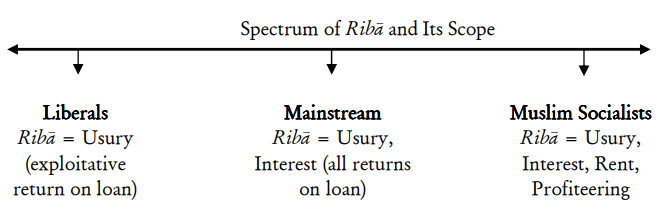
\includegraphics[width=\textwidth]{CourantsIslamContemporain/ImagesCourantsIslamContemporain/Riba.png}



The above differences have left scholars divided on several important questions that demand straightforward answers. Those questions include the following ones:
\begin{itemize}
    \item 
1. Is bank interest prohibited in the light of the Qur'an and the sunnah? If yes, how?
    \item 
2. Whether the Qur'anic term riba includes all kinds of interest rates or it relates only to the excessive interest rates?
    \item 
3. Whether the scope of riba extends to the interest charged and paid on business transactions in the banking system or is restricted to the interest charged on consumption loans only?
    \item 
4. Does Islam allow loan transactions? If yes, how and in what form?
    \item 
5. Is paying interest a lesser evil as compared to charging it?
    \item 
6. Is borrower always \textit{mazlum} (a losing party) in an interest bearing loan transaction?
    \item 
7. Does Islam allow indexation of loans on the grounds of inflation?
    \item 
8. Is credit-sale with higher deferred price as compared to the spot price allowed?
    \item 
9. Does Islam approve of “time value of money,” especially when charging higher deferred price is allowed in a credit sale?
    \item 
10. Are future currency contracts permissible in Islam?
    \item 
11. How and to what extent is salam transaction permissible?
\end{itemize}


These are but a few questions.
\begin{Synthesis}
We show in this paper that whatever confusion prevails among contemporary scholars on this subject is the outcome of following an inadequate methodology for determining the meaning and scope of riba.
\end{Synthesis}
 In fact, this methodology has mystified the nature of riba, which is otherwise clear when viewed from the methodological view point of the eminent Muslim jurists of the past. The mystification is such that not only it results in confusing answers to these questions but it also begets confusing questions. Unfortunately, the confusion has built up to the extent that the Federal Shariat Court of Pakistan has been struggling to come up with a definition of riba. It is in this background that this paper attempts to explain:

(1) the contemporary Islamic economists' methodology of interpreting and classifying riba; (2) why this methodology is wrong and insufficient; (3) the methodology of understanding riba on the pattern of Muslim jurists of the past; (4) that the methodology given by the Muslim jurists is coherent and compact.

The reader will encounter a number of arguments in this paper that are advanced by those who justify bank interest. Since the paper deals with the legal substance and not with the economic merits of arguments, hence we will restrict ourselves to the legal analysis of those arguments and leave aside their economic analysis and rationale, which require an altogether different methodology. Any legal system has three aspects: (1) what: the legal rulings (i.e., ahkam); (2) how: the rules of deriving those legal rulings (i.e., usul al-fiqh); and (3) why: the underlying rationale(s) and wisdom behind the legal rulings (i.e., hikmah)

It is important not to mix these aspects. The present study deals with the first two aspects of the issue of riba. Moreover, the classification of riba discussed in this paper is primarily based on the methodology of Hanafi jurists for ensuring analytical consistency. We presume that a school of law represents an internally coherent system of interpretation and that mixing up the views of the various schools results in inconsistencies.7 However, views of the other schools have been briefly mentioned in the footnotes wherever required. Finally, the paper does not attempt to show that the Hanafi jurists' approach is superior to all others, rather it explains that the classical jurists' approach (whether Hanafi, Maliki, Shafi‘i or Hanbali) to understanding riba is superior to that of the modern scholars. The methodology of these jurists share several common results that are important in order to answer the above questions.

Following section outlines the method adopted by modern Muslim scholars and economists. The next section discusses problems in this methodology and develops the skeleton for the methodology that is then applied in the coming section, which details out the general rules of riba alongside their resulting implications. The last section concludes the paper by giving a comprehensive definition of riba based on discussions in sections three and four.


\newpage
\subsection{Outline of the Mystifying Methodology}

Imran Ahsan Khan Nyazee\sn{\href{https://en.wikipedia.org/wiki/Imran_Ahsan_Khan_Nyazee}{Pakistan} Nyazee's academic career was inspired by the work of Abdur Rahim. Nyazee argues firstly, that due to its unique set of principles of interpretation, each school of Islamic law represents a theory of law unto itself. Secondly, he points out that Istiḥsān cannot be understood without understanding of the workings of qiyās. It is, therefore, difficult to accept that there was no system of interpretation before al-Shāfi‘ī's time. Thirdly, he concludes that the uṣūl al-fiqh never existed. Furthermore, Nyazee describes beyond the individual fikh of each school of law, another theory of interpretation called maqāṣid al-sharī‘ah (theory for the purpose of the sharī‘ah) which was developed by al-Ghazālī. Nyazee has written and self-published on a number of aspects of Islamic law. He agrees with most Muslim scholars that strictly speaking, selling money (taking interest) is prohibited, according to Islamic law. Some point out a difference between the treatment of riba in the Qur'an versus the Sunnah but Nyazee the two approaches are actually one and the same.Nyazee also proposes that all loans (except those of a charitable nature without a fixed period of repayment) and therefore all banking is prohibited and unIslamic. Nyazee is equally intolerant of murabaha, the Islamic system of business where in-put costs and mark-ups are made transparent between vendor and buyer. He argues riba will inevitably enter such transactions.[10] He extends the prohibition to the creation of wealth on the basis of debt and the fractional reserve banking system. These elements along with zakat (the system of alms-giving) he says, are the differences between Islam and capitalism. He advocates the use of the gold and silver dinars and dirhams as the currency of the Muslim community. Nyazee would also prohibit the corporation or 'legal personality' under Islamic law.} explains that the methodology adopted by modern scholars for determining the meaning of riba is the same, though they disagree in their conclusion regarding whether or not bank interest is riba.8 The fundamental problem of their methodology lies in overlooking the inherent link between the Qur'an and sunnah. This methodology of interpreting riba was initiated by Muhammad Rashid Rida (d. 1935) \sn{voir p. \pageref{Theol:Rida} Frère musulman pas le voyage en Europe. Plue el manar un commentaire coranique, sensé être l'héritage d'abdu}, which goes as follows:9

\paragraph{Lecture de Rida El Manar}
Riba is classified into two categories, riba of the Qur'an (also equated with riba 'l-nasi'ah, i.e., interest on loan transaction) and riba of hadith (equated with riba 'l-fadl, i.e., interest on exchange transaction).

Rida begins with literal meaning of the word riba (excess) and then traces some riba-based transactions practiced by Arabs during the time of Prophet (peace be on him). Rida, relying on some commentators of the Qur'an, asserts that the Qur'anic verse regarding riba deals with a specific practice of Arabs known as credit-sale where the payment of price is deferred to a future period while delivery of goods takes place on spot. Because a seller is allowed to charge whatever price he wants in a sale transaction, no riba is involved in the original price negotiated between the two parties-any excess in future price becomes part of the price. However, they used to increase the price excessively whenever the debtor would be unable to settle his debt obligations at the end of payment period. The debtor was given the option, “Will you pay the debt or increase the amount in lieu of delay?”

For Rida, it was this excessive rate (doubling and multiplying) of interest in debt-based transactions added to the original sum at the end of payment period which was prohibited by the Qur'an (he called it riba 'l-jahiliyyah).10 From this, he concluded that the bank interest is not the same riba that was deemed impermissible by the Qur'an because (a) it is neither doubling and redoubling of rates (b) nor the excess is stipulated in the initial period of the banking transaction-he assumes that the initially added interest is part of the principal or original sum just like the original sum in case of credit-sale. 
\begin{Synthesis}
Hence, for Rida, only compound interest is prohibited.
\end{Synthesis} 

Other scholars, supporting Rida's view, added that business loans were not common among Arabs as theirs was a subsistence economy; loans were largely taken by poor people for consumption purposes on interest and whenever they were unable to repay them at due time, excessive interests were added to the original sum. Hence, it was this type of interest that was declared prohibited by the Qur'an and it has nothing to do with the modern commercial loans, \textbf{which are mutually beneficial for both parties.}11

Having ascribed this meaning to the Qur'anic word riba on the basis of some historical traces, Rida then explains the form of riba declared impermissible in the sunnah as a distinct prohibition from that of the Qur'an.
\begin{Def}[Riba] Usure, profit ou gain réalisé sur un prêt.
\end{Def}

\begin{Def}
[Riba al-buyu] : Usure. Opération de vente dans laquelle une matière première est échangée contre la même matière première mais en quantité différente et la livraison d’une des matières premières est postposée. Pour éviter le riba al-buyu, les matières premières échangées par les deux parties devraient être en quantités égales et l’échange devrait être instantané. Riba al-buyua a été condamné par le Prophète Muhammad afin d’éviter que le riba (intérêt) n’affecte insidieusement l’économie.
\end{Def}
\begin{Def}[Riba al-duyun] : Usure d’une dette.
\end{Def}
 
\begin{Def}[Riba al-fadl] : La différence de quantité entre deux biens échangés et comportant du riba.
\end{Def}
\begin{Def}[Riba al-nasiah] : La différence de paiement liée au report de deux biens comportant du riba
\end{Def}\mn{cf Glossaire des termes financiers  Islamiques \href{https://www.cairn.info/la-banque-et-la-finance-islamiques--9782804167042.htm}{Banque et finance islamique} } He calls it \textit{riba 'l-fadl} which emerges in the exchange of two counter values of the same or different species and hence also called \textit{riba 'l-buyu‘}.12 The position of Rida, which may be termed as minority view, is summarised in figure 2.


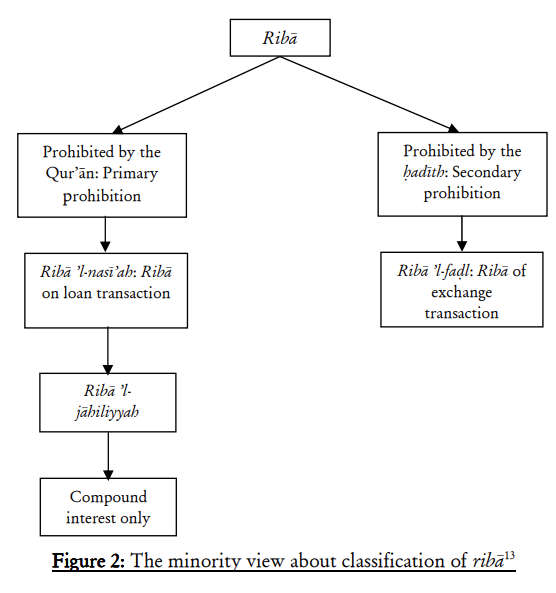
\includegraphics[width=\textwidth]{CourantsIslamContemporain/ImagesCourantsIslamContemporain/RibaRida.png}

Thus, Rida dichotomised the two concepts of riba, one attributed to the Qur'an and another to the sunnah. He finally declared the first one as real or explicit riba while latter as lighter or implicit riba.
\textbf{
Though the majority of contemporary scholars did not agree with the conclusion drawn by Rida about legitimacy of bank interest, however they adopted his methodology of classifying riba. The only difference in their opinion is that riba of the Qur'an includes all rates of return on loan and it is not merely restricted to the compound interest of jahiliyyah}\sn{la période pre islamique}


To them, business loans were a part of Arab's economy and any contractual return to lender is unfair because this is tantamount to refusing to share business risk with the borrower. We can depict their views in figure three.
\begin{Synthesis}
On a donc un nouveau problème, le pret commercial lié avec l'industrie et face à ce nouveau problème, une lecture de Rida qui est assez positive (Riba = Excess) mais qui note une différence entre Coran et Sunna) et fait une distinction entre les deux, reprises ensuite par les autres légistes, mais en repartant d'une lecture stricte du Riba comme intérêt. Il conveint d'articulier Coran et Sunna de façon non parallèle mais l'un par l'autre.
Il convient de montrer l'évolution du prêt commercial au XIX
\end{Synthesis}
Because the sunnah is not linked with the Qur'an in this methodology, both the minority and majority Muslim economists have struggled to explain as to why someone would engage in exchange transactions of the forms mentioned in hadith. Some opined that these transactions are declared impermissible because they may open the path for the “real riba” (i.e., riba of the Qur'an).


14 Others assumed that it was meant to discourage the practice of barter exchange and promote market exchange through a medium of exchange.15 Yet another view argues that it eliminates the possibility of benefiting from asymmetric information of the contracting parties.16 The truth is that none of these explanations makes the point.

2.1. The Nature of Debate within Minority and Majority Schools

The debate that has taken place within the followers of this mystifying methodology on the issue of why or why not bank interest is riba may briefly be summarised here. As explained above, Rida asserted that bank interest was not included in the Qur'anic concept of riba of debt because it was different from the riba that was charged by Arabs on credit-sale transaction by doubling and multiplying the price whenever the debtor was unable to settle his debt at due time and asked for relaxation in payment period.18 Rida explained that the Qur'anic verse “Allah has permitted bay‘ and prohibited riba”19 referred to this riba. To strengthen his case, he argued from the verse: “O Believers! Do not devour riba doubled and multiplied and fear God so that you may prosper.”20

This verse complements the former verse in the sense that what was implicit in the first verse was made explicit in the latter-both verses referred to the practice of doubling and multiplying of interest and none of them forbad the bank interest.

How do the majority of scholars respond to this argument? For example Usmani notes the Qur'anic verse:

O you believers! Fear God and give up riba that remains outstanding if you are true believers. Behold! If you do not obey this commandment, then God declares war against you from Himself and from His Prophet. But, if you repent (from riba), then you are entitled to only your principal amounts. Neither should you inflict harm to others, nor others should do harm to you.21

The argument is based on the emphasised words ‘you are entitled to only your principal amounts (ra's al-mal)'. He infers from these words that the rightful entitlement of lenders is the original sum advanced; he cannot charge any increase whether small or large (doubled and tripled). To him, the verse (3:130) forbids a severe form of riba where interest is multiplied, but it does not restrict riba to this specific form. Hence, bank interest falls within the purview of the Qur'anic verse “Allah has permitted bay‘ and prohibited riba.”22 They are also of the view that charging interest on commercial loans was also practiced by Arabs.23

Does the above analysis of mainstream scholars guarantee the prohibition of bank interest? We are afraid it does not. Their arguments rest on two assumptions:

(1) The verses (2:278-79) address the issue of loan-transaction.

(2) Ra's al-mal (principal amount) can only refer to the original principal advanced in loan.

Both of these assumptions are problematic. Following submissions can be made against them:

(a) If the meaning of the verse is to be determined with reference to historical practices, one can equally claim, just like Rida, that the verse is not about loan transaction but about credit sale. In that case, ra's al-mal is not referring to the principal amount lent; rather, it is the deferred future price of the goods sold. On which legal grounds or facts can this claim be dismissed?

(b) Further, this deferred price might include increase over and above spot price. Hence, the future price could consist of two components: spot price plus some additional profit. The sum of these two would constitute ra's al-mal (principal amount) in this transaction (i.e., principal amount in credit sale (ra's al-mal) = spot price + extra profit)

Whenever a debtor was unable to repay full amount, further multiplied increase was added to this original sum, Rida called it interest. This would increase the due amount to: total amount after increase added due to delay, which is interest in addition to ra's al-mal.

Using this structure, one can then argue that the initially added interest in a loan transaction is equivalent to initially added “extra profit,” which becomes part of ra's al-mal. Therefore, entitlement to the ra's al-mal means entitlement to the simple interest, as claimed by Rida.

(a) The only legal justification for ascertaining that the verse is about loan transaction is based on the words “ra's al-mal” (principal amount). But how can it be settled that ra's al-mal here means ra's al-mal of a loan transaction? This question is important because a number of transactions constitute a component of ra's al-mal. For example, there is ra's al-mal both in mudarabah and musharakah contracts. How to exclude these forms of ra's al-mal from the purview of the Qur'anic verse? If someone says, “This verse is about loan, so ra's al-mal refers to that of loan contract and not of mudarabah and musharakah,” he is clearly arguing in circularity. The argument goes like this:

Q: How do we know that the verse is about loan contract?

A: Because the verse talks about ra's al-mal.

Q: How do we know that ra's al-mal here refers to that of loan?

A: Because the verse is about loan contract!

A circular argument is no argument.

(b) Muslim Socialists could maintain that ra's al-mal means principal amount of all business contracts. Therefore, it is not legitimate to charge any excess over and above principal amount, no matter it is mudarabah, musharakah or ijarah.

Not only that the analysis of mainstream scholars does not necessarily imply the prohibition of bank interest, it leads to a set of unsettling arguments that have left Islamic economists bewildering about some basic issues. For example,

(1) Even if it is agreed that ra's al-mal means principal amount of a loan transaction, does it mean “nominal” amount or the “real” (inflation adjusted) amount? Again, what are the legal grounds to settle this issue? Because there are no clear-cut legal grounds available in this methodology, we see scholars are divided on this subject matter-some allow indexation of loan against inflations while others do not.

(2) What about the question of “time value of money?” This question poses challenge for Islamic economists because they, as a rule, approve the practice of charging higher price in credit-sale and murabahah.

(3) The Lawgiver has allowed salam, what are the legal grounds for not extending this permission to currency salam (future currency contracts)?

Undoubtedly, majority view has addressed these issues, but the answers do not seem to be stemming out of a coherent analytical legal system. This approach is often found mixing up legal analysis with economic analysis. This missing coherent analytical legal system is the root cause of most of the mystification that has prevailed all over. It is an unfortunate state of affairs and it is high time to demystify things.

3. Methodological Assumptions of Premodern Muslim Jurists (Fuqaha') for Understanding Riba

To understand the method used by the eminent premodern Muslim jurists for understanding riba, three methodological issues (MI) need to be clarified. They are explained by Nyazee in detail.24

1) Link between the Qur'an and Sunnah

The methodology adopted by the modern Muslim scholars and economists is misleading because it delinks the Qur'an and sunnah. It assumes that the meaning of riba is different in the Qur'an and sunnah, which is not the case. To explain the nature of error made by both the groups, it should be noted that Muslim jurists (fuqaha') classified riba in the category known as mujmal (unelaborated)25 whose meaning and scope cannot be determined without explanation (bayan) of the Lawgiver (Shari‘). The famous hadith (as given in footnote 1) that explains different usurious transactions actually does not add something to the Qur'anic word riba. Rather, it defines its meaning and scope.

Thus, while to the contemporary scholars the meaning of riba is known independent of hadith and they see hadith as adding some more cases to the Qur'anic concept of riba, the jurists say that hadith is the definition of the term riba used by the Qur'an. Thus, riba 'l-nasi'ah and riba 'l-fadl both are included in the Qur'anic concept of riba.

2) Relationship between Loan and Bay‘ (Exchange)

Loan is also classified as a form of exchange transaction (bay‘)26 by Muslim jurists. The scope of this paper does not allow detailed analysis of this assertion.27 For descriptive purposes, it can be seen that a loan of Rs X is an exchange of Rs X today with Rs X after time deferment (and with Rs X + Y if interest payment of Rs Y is included). Figure 4 depicts this nature of loan transaction by illustrating a loan transaction between Mr. A and B:

3) Skeleton of a Coherent Legal System

A coherent shari‘ah-based legal system consists of a set of general rules, called

‘azimah by the jurists, supplemented by some exemptions to these laws, called rukhsah. In the words of Nyazee, ‘Azimah (lit. determination, resolution) is applied to mean a rule that is applied initially and for itself. Such rules form the backbone of the law. As against this, there may be a rule that goes contrary to the requirements of the initial rule, but is permitted by the law. This rule is considered to be a rukhsah (exemption) from the initial rule.28

This classification of ‘azimah (the higher or first order rules) and rukhsah (the lower or second order rules) is important for several reasons.

First, it explains the order in which the rules have to be applied.

Second, it explains why sometimes two opposing cases may be allowed within a given skeleton of law.

Third, the order of rules implies that an exception cannot be extended using any method of argument, whether analytical or analogical. On the other hand, extension of first order rules is legitimate by these methods. In other words, it is not allowed to build a sub-legal system based on exemptions because otherwise it starts negating the primary provisions and objectives of the law-an exemption from the general rule must remain an exemption.

Fourth, because of the logical hierarchy in the operations of ‘azimah and rukhsah, it is clear that an exemption from a rule cannot be used to nullify or change the shari‘ah status (hukm) of any other case that is derived from the general rules. Alternatively put, an exemption (a lower order rule) cannot prevail over the higher order rules.

Fifth, because all rules and exemptions are derived from nusus (the Qur'an and sunnah), hence the only justifiable exemptions are the ones, which are given in nusus (i.e., stated by the Lawgiver Himself).

We call these nusus the “facts” of the shari‘ah-based legal system in this paper. Given these “legal facts,” the task of a jurist is to derive those general rules (‘azimah) from the facts, which render these facts internally consistent and extendible on the one hand and highlight the exemptions (rukhsah), if any, on the other.29 Finally, the general rules and exemptions generate some implications, called ahkam. This skeleton of a shari‘ah-based legal system is illustrated in Figure 5. We apply this skeleton in this paper to elaborate riba.

The relevant “legal facts” used by premodern Muslim jurists to derive general rules and exemptions are quoted at the relevant places in this article. We are now in a position to take on the issue of derivation of the general rules and the implications from those “facts.”

4. Underlying Rules behind the System of Bay‘ in Jurists' Methodology

Our intention in this paper is to reveal that the apparently large and complicated system of legal injunctions (ahkam) is reducible to a few set of rules derived from fewer legal facts. We propose that a majority of ahkam (legal injunctions or provisions) governing economic transactions (buyu‘) can be derived from three broad rules:

1. Rules of riba mentioned in the sunnah. This is not a single rule, rather a set of rules as explained below.

2. Rule about the sale of goods not possessed by a person.

3. Rule about exemption that an exemption is to be treated as exemption.

Before explaining these rules, we first explain the context of the Qur'anic verses that underlies the jurists' methodology of riba to clarify the misconception that the relevant verses of Surat al-Baqarah are about loan transaction and not exchange (bay‘).

4.1. The Context of the Verses of Surat al-Baqarah

The Qur'an states that the disbelievers said, “Verily, bay‘ (sale) is just like riba.” In response to this, it was said, “Allah has permitted bay‘ and prohibited riba.” To understand why the disbelievers said this, consider these three transactions:

(a) A gives B 100 grams of gold in exchange of 110 grams of gold to be paid after one year. This is primarily a sale contract as explained previously (i.e., exchange of 100 grams gold with 110 grams gold with time lag) and involves riba (how, this will be explained in the next section but take it for granted for the moment).

(b) A asks B for 100 grams of gold in exchange of, say, 500 kg wheat at spot. This is a legitimate regular sale contract.

(c) A demands from B 110 grams of gold in exchange of 500 kg wheat for payment of price after one year: this is credit sale contract with higher deferred price as compared to spot price and is also legitimate (this is explained in section 4.3).

The credit sale was a common practice among Arabs and, therefore, they were confused as to why the transaction (a) is impermissible and (c) is permissible while the two are quite similar in nature (i.e., both are credit sales and both involve access payment). In (a), 10 grams of additional gold are paid as counter-value for 100 grams of gold for a delay of one year and similarly 10 grams of gold are paid for a delay of one year in transaction (c). It is for this reason that disbelievers said, “Verily sale is just like riba!” That is, transaction (c) (i.e., the credit sale) is similar to the transaction (a). The technical reason for allowing transaction (c) and forbidding (a) is the similarity of genus which is explained by the sunnah. This is explained in the next sections in detail, but the important point to note here is that the assumption that the Qur'anic term riba is not about sale contract, rather it is about debt, is not implied by these verses.

Thus, the verse says that Allah has approved all forms of buyu‘ (exchange transactions) except those which involve riba.30 The natural question then arises: what is this thing called riba? Has the Qur'an given any definitive description of riba?

One may make one of the two assumptions here. First, the concept of riba was largely a sort of common knowledge for everyone and, hence, it required no legal description by the Qur'an. That common knowledge is traceable by an examination of historical record of Arabs which provides sufficient legal foundations for determining the meaning of riba. As far as the details of riba in the sunnah are concerned, they were additions over and above to that common knowledge of riba and most of these additions were unknown to the Arabs. The liberals and mainstream scholars share this assumption and we believe that this assumption constitutes what we called the “mystifying methodology.”

Second, some forms of riba may be or actually known to the Arabs but these do not set the legal standard against which the Qur'anic concept of riba is to be determined. As it is a legal term, its meaning has to be sought from the Lawgiver. In technical sense, the jurists call it mujmal (unelaborated) for which elaboration (bayan) is sought from the Lawgiver. This elaboration of the legal meaning of the Qur'anic term riba is given by the sunnah. After this elaboration by the Lawgiver, its meaning is determined definitively and it becomes mufassar (elaborated). This is the methodological assumption that the jurists use not only for defining riba but also for other legal terms of the Qur'an, such as salah, zakah, and so on.31 Thus, according to this second assumption, the practices and concepts of Arabs may be referred by the Qur'anic concept riba but it is not the benchmark against which we assign legal meaning to the Qur'anic terms.

For example, the Arabs had some concepts about how to offer salah (prayer), but this information does not define the legal meaning of the Qur'anic term salah nor is this concept limited to this information set. Similar is the case with riba. The Arabs might have been aware of some forms and practices of riba but that does not constitute the legal definition of riba. When the jurists classify a term as mujmal, they mean that this term is a technical legal term and its meaning should be determined with reference to the words of Lawgiver Himself, neither by the linguistics (dictionary) nor by the historically known social concepts and practices that hover around that technical term. It should be emphasised here that considering riba as mujmal does not mean that the Arabs did not know the meaning of this word at all. Nor does it mean that the pre-Islam Arabs did not identify certain transactions as riba-in fact they did and the jurists did consider it part of riba.32

It only means that the meaning of riba in Islamic law is not limited to, and is not based on its usage in the pre-Islam Arabia. The Qur'an and the sunnah added several shades of meaning to this concept. That is why, it became a “technical term” of Islamic law. Hence, its meaning and scope cannot be determined by its dictionary meaning or its practice and understanding by the pre-Islam Arabs. Rather, it must be determined by the Qur'an and the sunnah, like any other legal term such as salah and zakah. Just as we cannot classify concept salah as salah of the Qur'an and salah of hadith, similarly we cannot dichotomise riba. Once it is established that the meaning of riba must not be gathered from pre-Islamic usage and practices but from the Qur'an and the sunnah, the next question is: how to explain the various usages of riba in the Qur'an and the sunnah? The answer, as per the well-established methodology of the jurists, is to consider the sunnah as the elaboration of the mujmal verses of the Qur'an.

This methodology is employed by the jurists for determining the meaning and scope of salah and zakah as well as riba. Let's follow through the path of righteous ones here and have its blessings.

4.2. General Rules of Riba When Transacted Species are Same

Keeping these in mind, one has to understand the classification of riba in the system of Muslim jurists. Because the sunnah defines riba, note the words of hadith,

When you exchange gold for gold, silver for silver, wheat for wheat, rice for rice, dates for dates, and barely for barely, then exchange like for like (in equal measure) and exchange them hand to hand (at spot), else it will be riba.33

To understand what it says, consider these transactions:

1) exchange of 1 gram gold for 1 gram gold on spot;

2) exchange of 1 gram gold for 2 grams gold on spot;

3) exchange of 1 gram gold at spot for 1 gram gold with delay;

4) exchange of 1 gram gold at spot for 2 grams gold with delay.34

As per the hadith, the first transaction is allowed; the second one is disallowed because it involves excess in measurement/quantity (called riba 'l-fadl); the third transaction is also impermissible because the hadith says that the exchange of homogeneous goods is allowed in equal measurement provided it is on spot; therefore, this transaction involves the riba 'l-nasi'ah (i.e., riba of delaying); finally, the fourth transaction involves both types of riba. These transactions provide two guiding rules (R):

R 1.1) Goods of the same species cannot be exchanged immediately unless their measurement (in terms of weight or volume) is same.

R 1.2) Goods of the same species cannot be exchanged with time lag, even with same measurement.

4.2.1. Implications

Five important implications (I) should be noted.

I. 1) Impermissibility of Market for Loanable Funds

Application of rule 1.2 gives the important implication that loan, with or without interest, is prohibited in Islam because, as explained above, a loan is an exchange of homogeneous goods with time lag. Does it mean that loaning is not allowed in Islam under any circumstances? Of course, this implication of the general rule is at odd with a number of legal facts (nusus), which promise reward for offering loan to the needy ones. How to reconcile these apparently contradictory legal facts now? This is where the concept of rukhsah (exemption) is activated by the jurists. Though loaning is against the general rule (‘azimah) given by the Lawgiver, yet it is allowed by Him as an exemption from this prohibition if it takes the form of benevolent giving (tabarru‘ or sadaqah).35 Loan is classified as tabarru‘ if:

(a) it is out of the intention of benevolence to the other person (i.e., the lender consciously bestows upon the borrower the benefits associated with his asset);36

(b) no increase in its value is stipulated, else it would cease to be benevolent and would involve riba 'l-fadl; and

(c) no contractual time limit is stipulated, the lender can ask for his asset anytime he wants.37 Stipulating (legal) time constraint in loaning activity makes it a business transaction as per the application of general rules of shari‘ah and, hence, unlawful because in that case it is simply the exchange of homogeneous goods with time delay, which is not allowed, whether or not interest factor is included. Moreover, making the time period binding would imply that the lender is forced to do, or to continue with, an act of charity. This is against the very nature of charity.

In short, this principle implies that Islamic law does not permit the “market for loanable funds.” It sees loaning as an act of benevolence, especially in favour of one's relatives.38 Stated alternatively, loan is purely a social transaction (a means of tying and strengthening social bonds) in Islam and not a business. It was in this social transaction capacity that the institution of loan prevailed for thousands of centuries not only in Muslim societies but also in other civilisations of the world until the emergence of capitalism in the fifteenth century.39 Note that this important result (impermissibility of the market for loanable funds) does not follow directly from the classification of modern scholars of Islamic economics, as the majority view allows interest-free non-benevolent loans as a general rule and not as an exemption.

This implication answers one of the important arguments in favour of bank interest given by some economists. The argument says that interest should be allowed in shari‘ah because interest is the price of capital and without interest the market for loanable funds cannot be equilibrated. Because we are not dealing with the economic merit of arguments in this paper, we ignore its economic substance and comment on its legal merit only. It is clear from the above implication now that this argument has no shari‘ah basis because shari‘ah does not allow market for loanable funds to begin with, let alone equilibrating it from shari‘ah perspective.

Before moving on to the next implication, the important implication and exemption regarding loan transactions be noted:

I 1.1) A loan transaction is prohibited, whether or not interest factor is added to it.

I 1.2) A benevolent interest-free loan is recommended as an exemption to the general rules of riba by the Lawgiver.

I. 2) Impermissibility of Bank Interest

All forms of bank interest, whether simple or compound, are prohibited by Islam as per Rules 1.1 and 1.2. Similarly, the fact whether loan is made for business or consumption purposes makes no difference to this result. There remains no confusion about these conclusions if the shari‘ah rules are applied with consistency. In fact, the practice of charging interest by the bank includes both kinds of riba and it, therefore, may be stated that it is the most comprehensive form of riba! This can be verified from the figure 6, which depicts detailed structure of riba-based transactions in case of homogenous goods (leaves aside heterogeneous goods for the moment).

I. 3) False Dichotomy between “Giving and Taking” Riba

The recipient of riba is not always the lending party as is usually perceived. It can be seen from above examples that in case of transaction (2) the lender is the beneficiary of riba, but in transaction (3) riba is received by the borrower, and finally both are its recipients in transaction (4). Hence, opinions such as “taking riba is a greater evil than giving it and, hence, paying interest to the bank is a lesser evil” are based on the fallacious assumption that it is only the bank that receives interest in a typical interest-bearing loan transaction. This wrong assumption is the outcome of using the wrong methodology outlined in section two.40

I. 4) Mutually Beneficial Riba is Prohibited

The view that bank interest realised in transaction (4) is or should be permitted (as claimed by liberal Muslim scholars) is implicitly based on the assumption that “two wrongs make one right”-that is, it assumes that mutually enjoyed riba of the lender and borrower can make this transaction acceptable while the matter of fact is that each of them is separately prohibited to begin with.

I. 5) Irrelevance of Time Value of Money

Following the wrong methodology has resulted in another confusing argument that the bank interest should be allowed because of “time value of money.” This argument is based on the presumption that Rs. 1 today is worthier than Rs. 1 tomorrow. Why? Economists believe that this is due to the subjective time preferences of an individual. A rational (i.e., self-interested utility maximising) economic agent is said to have positive time preferences in the sense that consumption today is preferred to consumption tomorrow because the latter is uncertain, which makes him impatient, thus he wants to have it today than tomorrow.

Another reason for having this positive time preference emerges from the institutional arrangements: if I have the option of earning some interest (say Rs. Y) on Rs. 1 by putting it in a bank account today, why should I lend it to someone for free? Putting Rs. 1 in a bank account will make it “Rs. 1 + Rs. Y” for sure (assuming away bank insolvency), say, after one year while lending it to someone will leave it worth Rs. 1. Hence, Rs. Y (which may be expressed in percentage) is the price that should be paid to the lender for a loan of one year, else it would be unfair with him. This argument is more of economic than legal in its substance, however, some comments can be made here to evaluate its legal substance in the light of preceding discussion.

The relevant part of the proposed argument is the second one (the institutional arrangement) because the first one is merely a subjective feeling, which may differ from person to person (as a matter of fact, not everyone prefers to consume more today than tomorrow). The argument presumes that there exists and should exist a well-established legally functional market for loan, which coordinates interest-based loan transactions. But just recall “I.1” that Islam does not approve of the market for loan to begin with. Eliminate this institution of market for loan, and the argument disappears. The point is that the concept of “time value of money” conceived in this economic sense is alien to the discussion of riba. Its validity presumes that there exists a legal institutional market for loanable funds where money is growing continually and, therefore, an individual always has the option of putting his money in that market.

Not only that this assumption is invalid from the point of general rules of shari‘ah as explained, it is also in contradiction with the ontological structure of the universe and economic facts.

The above is not the only format of this argument, it is phrased in some other shades as well. For example, it is stated that money could buy benefits and had the lender not lent it he could have benefitted himself. This implies that lending is an act of sacrificing the benefits associated with money. Therefore, the lender should be compensated for this sacrifice and interest payment is exactly that reward. This reward makes sense given that the borrower takes benefit out of money. The argument is valid to the point that money is beneficial to the lender and that if he makes the choice of not lending it, he can benefit from it. Moreover, it is also true that the borrower enjoys the benefits associated with the money. None of these facts is denied by the shari‘ah rules. But these facts alone cannot formulate the required case for this argument; it requires a moral statement in its premise to derive the desired conclusion.

To see this, note that the argument does not end here, after quoting these facts it then makes a moral assertion: “it is morally (and hence legally) right if money is lent for reciprocal benefits.” Addition of this moral statement is necessary for validating the conclusion that “interest is the just reward for lending.” But this moral assumption contradicts the general rules of the shari‘ah, which are laid down above. Seeking reciprocity in loan is exactly what that changes its status from tabarru‘ to loan as a business transaction and, hence, it becomes nothing but riba. The argument here is quite straightforward:

The owner of money is granted the right of benefitting from his money by shari‘ah rules; he is given the option of making a conscious choice of transferring the benefits associated with his money to another person as an exception to the general rules by the shari‘ah, but there is neither any general rule nor any exemption from the Lawgiver that assigns him the right of lending money in the name of the so-called “mutual benefits” (refer to I. 4 above). Legally speaking, this involves both riba 'l-fadl (because the homogeneous goods are exchanged at different rates) and riba 'l-nasi'ah (because time stipulation is invoked-the lender asks for the excess of measurement for parting with the benefits of his money for a specified time).

Another variant of this argument comes with the heading of “effects of inflation on money.” We deal with it in the next section.

4.3. General Rules of Riba when Transacted Species are Different

What about the exchange of heterogeneous goods? The last words of the hadith are as follows: “If these species differ, then exchange as you like as long as it is from hands to hand.”

They give an immediate rule:

R 1.3) Goods of the different species can be exchanged with difference in measurement.

This rule says that such goods can be exchanged at different rates as far as measurement is concerned. In other words, riba 'l-fadl does not apply in case of heterogeneous goods. Is riba 'l-nasi'ah (prohibition of time delay in payment) also not applicable in this case? Apparently, it seems that it is not because of the words of hadith, “exchange should be on spot.” This has an odd implication that credit sale (sale of goods against money where payment is deferred to future time period) is not permissible under the shari‘ah rules. This is so because credit-sale is an exchange of heterogeneous goods with time lag. But the legal facts reveal that the Lawgiver has allowed credit-sale.41 How to explain this? Is credit sale also an exemption to the general rule, like a loan transaction? The answer is: “No, it falls within the general rules.”

To see how credit-sale is permissible within general rules, one needs to dig deep into the issue of the underlying cause (‘illah) that the Muslim jurists derived from the sunnah to understand the system of riba. The relevant question facing jurists was: Is prohibition of riba restricted only to the six goods named in the hadith or is it extendible to other goods? The answer of the jurists is, yes, it is extendible and for this extension they derived the underlying cause due to which riba was declared prohibited by the Lawgiver. Keeping aside the technical details and arguments, it should be noted that some of the goods are measured in terms of weight while others are measured in terms of volume. In the hadith under discussion, gold and silver were weighable while the other four items were volumeable at the time of Prophet (peace be on him).42 Based on this classification, the jurists derived two further rules:

R 1.4) when species are different but their method of estimation is the same (such as gold vs silver or wheat vs rice), unequal quantities can be exchanged, provided that the exchange is immediate;

R 1.5) when species are different and their method of estimation is also different (such as gold vs wheat), unequal quantities can be exchanged with time delay.43

Thus, the credit sale is allowed due to the application of Rule 1.5. To see this, consider these combinations of transactions:

1) Exchange of 1 gram gold at spot for 2 gram silver on spot (method of estimation same)

2) Exchange of 1 gram gold at spot for 2 gram silver in future (method of estimation same)

3) Exchange of 2 kg wheat at spot for 1 gram gold/silver on spot (method of estimation different)

4) Exchange of 2 kg wheat at spot for 1 gram gold/silver in future (method of estimation different)

The first transaction is allowed but the second is not because when species are measured by same method (i.e., “weight” in this case), then difference in the measurement (fadl) is allowed but deferment (nasi'ah) is not permissible. The third and the fourth transactions are allowed because here not only the transacted species are different but also their method of measurement (one was measured in “weight” while the other in “volume”).

In short, when both of the similarity factors (i.e., species and method of measurement) are found, then both fadl (excess of measurement) as well as nasi'ah (excess of time delay or time deferment) are prohibited. When similarity of measurement is found alone, then fadl is allowed but nasi'ah is prohibited. Finally, when none is found, both fadl and nasi'ah are allowed. Figure 7 depicts all of these rules completely (discussion about the last layer of boxes on the right-hand side of this figure is coming next).

The preceding discussion shows that the hadith explaining the nature of riba was not about the actual practices of Arabs that begged some economic explanations with which Muslim scholars have been struggling. Rather, it stipulated the rules of exchange. It says, “If at all you make exchange transactions, here are the governing rules.” Thus, all transactions that correspond to these general rules are allowed while those in contradiction with them are prohibited (however, some are exempted by the Lawgiver).

4.3.1. Implications

Following implications are derived from the above rules. It is important to note that the first two transactions mentioned in sub-section 4.2 belong to the case when method of estimation of the heterogeneous goods is same while the latter two cover the cases when their method of estimation is different.

I. 6) Placement of Regular and Credit-Sale

Transaction (3) is categorised as regular sale transaction (usually termed bay‘) by the jurists. On the other hand, transaction (4) covers credit sale, which may take two forms: with or without extra profit margin as compared to the spot sale. Because both measurement as well as payment time differential are allowed in this case, hence credit sale of both forms is allowed.

I. 7) Placement of Currency Exchange

The remaining two boxes are relating to the exchange of currencies (termed as bay‘ al-sarf by the jurists). A detailed description of these requires an appreciation of some more technical classifications44 made by the Muslim jurists. However, they are beyond the scope of this paper. Suffice to say that the jurists divided all tradeable species into two: (a) currency items, which are used as means of exchange; they included gold and silver (though other goods may also be treated as currency in this system) and (b) non-currency items, (goods that are exchanged, and are not medium of exchange). They roughly included all but gold and silver.45 Given this division, the jurists broadly mention four types of transactions (buyu‘):

(1) Non-currency item in exchange of non-currency item-called barter exchange.

(2) Spot or delayed currency (say gold) in exchange of spot non-currency (say wheat) item.

(a) If both of them (gold and wheat) are exchanged on spot, it is called regular sale of goods, and

(b) if the currency price (gold) is delayed, this is called credit sale.

(3) Delayed non-currency item (say rice) in exchange of spot currency item (say gold). Here, the price of the good is paid on spot while its delivery is delayed. This is called bay‘ al-salam (advance payment) by the jurists.

(4) One currency (gold) in exchange of another currency (silver)-known as bay‘ al-sarf.

Rules regarding the first two have been discussed above. Here, we have to make some submissions regarding this fourth type of transaction. Because this transaction comes under the umbrella of “different species with same method of measurement,” it is clear from figure 7 that the excess of measurement is allowed in this transaction while time deferment is not. This gives two further rules under rule (1.4):

1.4a) If different currency items (such as gold and silver) are exchanged, then it is allowed to exchange them at any rate;

1.4b) if different currency items (such as gold and silver) are exchanged, then it is not allowed to exchange them with time deferment.

If it is accepted that modern currencies are just substitutes of gold and silver, then two further important results emerge from this discussion:

I 7.1) Future Currency Contracts are Prohibited

Rules (1.4a) and (1.4b) imply that the spot currency transactions are allowed while their future contracts (known as currency salam in Islamic finance literature) are prohibited in Islam as they come under the purview of riba 'l-nasi'ah.

I 7.2) Indexing of Loans is Prohibited

Indexing the value of the currency loans against some underlying assets (say gold) on the ground of inflationary pressures is not allowed. It is often argued that since the value of currency decreases over time due to the presence of inflation, hence an extra-payment equal to the rate of inflation, over and above the original sum given in loan, should be allowed in favour of the lender to keep his purchasing power. Again, because the economic merit of this argument is beyond the scope of discussion in this paper, we restrict only to its legal merit. If it is accepted that one rupee is legally nothing but equivalent of 1 unit of gold or silver (whatever that unit be), then Rules 1.1 and 1.2 (governing the loaning contract in gold or silver currencies) should automatically become operational.

Those rules imply that (a) loaning in the form of currency item is allowed if and only if equal measurement (whatever the unit of measurement) is returned; else it would be riba 'l-fadl; and (b) it is a loan made out of benevolence and not business intention (having time stipulation); else it would be riba 'l-nasi'ah. Hence, adding an extra amount to loan transaction in the name of “indexation” is but both, riba 'l-fadl (because of the excess of measurement) and riba 'l-nasi'ah (because the increase is time bound). 46 Again, let simplicity and sanity prevail.

I. 8) Placement of Salam

To see how the jurists accommodated salam in this scheme, note that there is nothing in the set of rules 1 (from 1.1. to 1.5) which forbids it. However, according to rule 2 (given at the start of this section), selling what one does not possess is not permissible and this is exactly what a salam transaction involves. Thus, a salam transaction should not be allowed as per the general rules of shari‘ah. We are once again faced with the same issue: salam is permitted in the “legal facts;” how and where to place it in the legal skeleton of the shari‘ah? Is there another general rule, which governs its permission as we saw in case of credit sale or is it an exemption from the general rule just like loan? The jurists' answer is the following: Salam is permitted as rukhsah-exemption from the general rules-by the Lawgiver.47

Because it is an exception, as per rule 3, it would be allowed only as “one of its kind” (sui generis) and cannot be used as justificatory mode for deriving more comparable transaction forms (e.g., currency salam). An exception to the general rule remains exception and does not turn into a rule for other cases because then it ceases to be an exception and creates a situation of self-contradictory general rules, which is not acceptable in any legal system. Thus, salam transaction is allowed as an exception for those transactions where (a) a currency item is exchanged against a non-currency item and (b) non-currency item is deferred while the currency-item has been paid at spot.48 This is what the exception is all about; one cannot extend this exception to the transaction types where currency items are exchanged with each other because that would violate condition (a) of the exception case.49

Figure 8 shows a map of interplay among legal facts (nusus), general rules, exemptions, and the derived implications related to riba and bay‘ that are discussed in this paper. This diagram shows that a rather complex looking system of ahkam (implications) showing up at the ending layer boxes of figure 8 emerge out of a set of general rules, which are derived to make underlying legal facts compatible with each other.

5. Conclusion: The Definition of Riba

We conclude this paper by elaborating a comprehensive definition of riba that can be inferred from the discussions in this paper. Let's quote it from al-Sarakhsi:50
\begin{Synthesis}
Riba in its literal meaning is excess... and in the technical sense (in the shari‘ah), riba is the stipulated excess without a counter-value in bay‘ (sale).51
\end{Synthesis}


Let's explain it noting several points about this definition:

(1) Muslim jurists do not introduce the word loan in the definition of riba because they categorise loan transaction under exchange (bay‘). Not appreciating this point resulted in the misconception that since the fiqh conception of riba does not deal with the subject of bank loans, it needs to be inferred directly from the Qur'an.

(2) Riba is excess, either in the form of quantity (qadr) or in the form of benefits of delay (nasa'). The first is called riba 'l-fadl while the latter is called riba 'l-nasi'ah.

(3) This excess is without any counter-value permitted by the shari‘ah. Thus, the excess of quantity paid in lieu of time delay in case of interest-bearing loan is not allowed because these two cannot be the legitimate counter-values (see I. 4).52 For a substance to be counted as counter-value, it must be recognised by the general rules of the shari‘ah to begin with.53

(4) The excess is stipulated in exchange. If the excess is granted voluntarily, it would not be riba.

We started off with specific questions in the introduction. The appendix lists down the answers to these questions in the light of the above definition of riba. It can be seen that once the discussion about riba is placed on the right track, right and clear cut answers start emerging automatically.

Appendix: Questions and their Answers that Follow from the above Analysis

Notes

1 For detailed arguments of this position, see Abu 'l-A‘la Maududi, Sud (Lahore: Islamic Publications, 2000), 110-12; M. Umer Chapra, “The Nature of Riba in Islam,” Hamdard Islamicus 7, no. 1 (1984): 3-24; Muhammad Shafi‘, Mas'alah-i Sud (Karachi: Idarat al-Ma‘arif, 1996), 43-47; Muhammad Ayub, “What is Riba? A Rejoinder” Journal of Islamic Banking and Finance 13, no. 1 (1996): 7-24; Muhammad Taqi Usmani, The Historic Judgment on Interest Delivered in the Supreme Court of Pakistan (Karachi: Idarat al-Ma‘arif, 1999), 12-16; Mohammad Nejatullah Siddiqi, Riba, Bank Interest and the Rationale of Its Prohibition (Jeddah: Islamic Research and Training Institute, 2004), 45-48; and Mahmoud A. El-Gamal, Islamic Finance: Law, Economics, and Practice (Cambridge: Cambridge University Press, 2006), 46-52. Within this category, there are further two approaches.

One approach that represents traditional ‘ulama' emphasises the resurgence of only those business contracts that were approved by the early Muslim jurists. It proposes profit-and-loss sharing (PLS) as an ideal alternative to riba. Though it does not deny the permissibility of other than PLS-based financing instruments such as murabahah and ijarah, yet it affirms that equity-based financing method is the primary means of achieving desirable economic objectives. The second approach is pragmatic one. It justifies a more liberal and flexible stance on structuring shari‘ah-compatible transaction forms that looks for financial engineering to meet all demands of modern banking customer.

2 Muhammad Rashid Rida (d. 1935) was among the foremost proponents of this theory. See his al-Riba wa 'l-Mu‘amalat fi 'l-Islam (Cairo: Dar al-Manar, 2007). Also see Sayyid Yaqub Shah, “Islam and Productive Credit,” The Islamic Review 47, no. 3 (1959): 34-37; Fazlur Rahman, “Riba and Interest,” Islamic Studies 3, no. 1 (1964): 1-43; Timur Kuran, “On the Notion of Economic Justice in Contemporary Islamic Thought,” International Journal of Middle East Studies 21, no. 2 (1989): 171-91; Izzud-Din Pal, “Pakistan and the Question of Riba,” Middle Eastern Studies 30, no. 1 (1994): 64-78; and ‘Abd al-Karim Athari, Sud Kiya Hay? (Mandi Baha' al-Din: Anjuman-i Isha‘at-i Islam, 2008), 8-12 3 Constant J. Mews and Ibrahim Abraham, “Usury and Just Compensation: Religious and Financial Ethics in Historical Perspective,” Journal of Business Ethics 72, no. 1 (2007): 1-15.

4 See Ghulam Ahmad Parvaiz, Nizam-i Rububiyyat (Lahore: Idara-i Tulu‘-i Islam, 1978).

5 Rafi‘ Allah Shihab, Kirayah-i Makanat ki Shar‘i Haithiyyat (Lahore: Kitab Ghar, 1981).

6 Ziaul Haque, “The Nature and Significance of the Midieval and Modern Interpretations of Riba,” The Pakistan Development Review 32, no. 4 (1993): 933-46.

7 For details, see Imran Ahsan Khan Nyazee, Theories of Islamic Law: The Methodology of Ijtihad (Islamabad: Islamic Research Institute, 1994), 9-12.

8 Nyazee, The Concept of Riba and Islamic Banking (Islamabad: Institute of Advanced Legal Studies, 1995), 11-19. Imran Ahsan Khan Nyazee (b. 1945) is a well-known scholar and a prolific writer on the subject of Islamic law and is a former Professor of law in International Islamic University, Islamabad. His major works include Theories of Islamic Law; Islamic Jurisprudence; Islamic Law of Business Organization; and The Concept of Riba and Islamic Banking. He also translated some of the classical texts on Islamic law and jurisprudence, including: Hidayah of Marghinani; Bidayat al-Mujtahid of Ibn Rushd; Amwal of Abu ‘Ubayd; and first two volumes of Muwafaqat of Shatibi.

9 Rida, al-Riba wa 'l-Mu‘amalat fi 'l-Islam, 69ff.

10 Period before the advent of the Prophet (peace be on him) is referred to as jahiliyyah (i.e., the period of uncivilised state of affairs).

11 Fazlur Rahman, “Riba and Interest,” 7-8.

12 In this regard, a hadith reads, “The Prophet said, ‘While exchanging gold for gold, silver for silver, wheat for wheat, barley for barley, dates for dates, and salt for salt, exchange like for like, in equal measure, and exchange from hand to hand. If these species differ, then sell as you like as long as it is from hand to hand.'” Muslim b. al-Hajjaj, Sahih, Kitab al-musaqah, Bab al-sarf wa bay‘ al-dhahab bi 'l-wariq naqdan.

13 Adopted from Nyazee, Concept of Riba.

14 Maududi, Sud, 118-19.

15 Chapra, “Nature of Riba in Islam,” 3.

16 Siddiqi, Riba, Bank Interest and the Rationale of Its Prohibition, 49-50.

17 Adopted from Nyazee, Concept of Riba.

18 Rida, al-Riba wa 'l-Mu‘amalat fi 'l-Islam, 69-70.

19 Qur'an 2:275.

20 Ibid., 3:130.

21 Ibid., 2:278-79.

22 Ibid., 2:275.

23 For details, see Shafi‘, Mas'alah-i Sud, 106-120 and Siddiqi, Riba, Bank Interest and the Rationale of Its Prohibition, 38-40.

24 Nyazee, Concept of Riba, 35-36.

25 Mujmal is a term used by Muslim jurists to refer to a Qur'anic term that begs its explanation through the words of Lawgiver (i.e., God and His Prophet [peace be on him]). One cannot interpret mujmal either by looking its meaning in the dictionary nor can its meaning be determined through historical practices at the time of revelation of the Qur'an. Mujmal can be elaborated only by the Lawgiver. Another example of mujmal is the Qur'anic term salah (prayer) which cannot be interpreted literally.

26 Bay‘ means exchange of counter values, and is not restricted to sale of goods/services. Abu Bakr b. Mas‘ud al-Kasani (d. 587/1191), the illustrious Hanafi jurist, defines bay‘ as “exchange of property with property” and then elaborates that the concept includes not only ordinary sale but also barter, exchange of currencies, advance payment and many other forms of exchange. Bada'i‘ al-Sana'i‘ fi Tartib al-Shara'i‘, ed. ‘Ali al-Mu‘awwad and ‘Adil ‘Abd al-Mawjud (Beirut: Dar al-Kutub al-‘Ilmiyyah, 1997), 6:532-33. Abu 'l-Hasan ‘Ali b. Abi Bakr al-Marghinani (d. 593/1197), author of the authoritative Hanafi manual al-Hidayah, also explicitly asserts that qard (loan) begins as an act of charity but becomes an exchange transaction in the end. al-Hidayah fi Sharh Bidayat al-Mubtadi (Beirut: Dar Ihya' al-Turath al-‘Arabi, n.d.), 3:60

27 See Nyazee, Concept of Riba, 45-46.

28 Ibid., 49.

29 The Hanafis use the methodology of istihsan (juristic preference) for ensuring harmony and analytical consistency within the law when general rules and legal facts seem to contradict. If something appears prohibited in the light of the general principles of law, but has been explicitly permitted by one of the texts (i.e., legal facts), the Hanafi jurists take the position that it is permissible as an exception to the general principle. They use the rule, “prohibited under qiyas but permissible under istihsan” for this purpose. Exceptions to the general principles are made on the basis of the text, consensus, necessity or some other “covered principle” (qiyas khafi), which needs to be uncovered. Muhammad b. Abi Sahl al-Sarakhsi is worth quoting here: “This [istihsan] is the evidence coming in conflict with that apparent principle (qiyas zahiri), which comes into view without one's having looked deep into the matter.

Upon a closer inspection of the rule and the resembling principles, it becomes clear that the evidence that is conflicting with this apparent principle is stronger and it is obligatory to follow it. The one who chooses the stronger of the two evidences cannot be said to be following his own personal caprices.” Muhammad b. Abi Sahl al-Sarakhsi, Tamhid al-Fusul fi 'l-Usul, ed. Abu 'l-Wafa' al-Afghani (Beirut: Dar al-Kutub al-‘Ilmiyyah, 1993), 2:200-202. Another important point made by al-Sarakhsi is that when the jurist uses istihsan and prefers the stronger rule, he abandons the weaker one and as such it is not permissible for him or his followers to follow the latter. He goes on explaining that when istihsan is carried out on the basis of a concealed or covered principle (qiyas khafi), the established rule does not amount to be an exception but becomes a general principle in itself.

Interestingly, not only the Hanafi jurists but also the Maliki jurists explicitly employ the principle of istihsan for resolving the apparent anomaly found in the legal facts where one set of nusus prohibits a loan transaction and another set of nusus allows it. They hold that it is prohibited as an exchange transaction but allowed as an act of charity.

30 Al-Sarakhsi interprets this verse as the following: “Trade is of two kinds: permitted (halal), which is called bay‘ in the law; and prohibited (haram), which is called riba. Both are types of trade. Allah informs us, through the denial of the disbelievers, about the rational difference between sale (bay‘) and riba, and says, ‘That is because they said, “Sale is like riba.”' He, then, distinguishes between prohibition and permission by saying, ‘And Allah has permitted sale and prohibited riba.' Through this, we came to know that each one of these is trade, but only one form is permitted.” Al-Sarakhsi, al-Mabsut, ed. Hasan Isma‘il al-Shafi‘i (Beirut: Dar al-Kutub al-‘Ilmiyyah, 1997), 12:1-2.

31 The famous Hanafi jurist Abu Bakr al-Jassas al-Razi (d. 370/980) says, “In the law (shari‘ah), it (riba) is applied to meanings in which it was not used in the language. This is indicated by the fact that the Prophet (peace be on him) termed nasa' as riba in the tradition of Usamah b. Zayd (God be pleased with him). He said, ‘Verily, riba is in nasi'ah.' ‘Umar b. al-Khattab, (God be pleased with him) said that riba had different forms and out of these salam in teeth, that is, in animals, is not concealed. ‘Umar also said that the verse of riba was one of the last to be revealed, and the Prophet (peace be on him) was taken away before he could elaborate the details for us. Therefore, give up riba and the suspicion of riba. It is established from this that riba became a technical term, for had it been governed by its original meaning in the language, it would not have been obscure for ‘Umar, who was fully aware of the names used in the language, being a native speaker.

This (the conversion of the word into a technical meaning) is also indicated by the fact that the Arabs were not aware of the sale of gold for gold and silver for silver with a delay (nasa') as riba, but this is riba in the technical meaning. If this (meaning of riba) is as we have explained it, then, it became like all the other unelaborated (mujmal) words that are in need of an elaboration (bayan). These are terms that have been transferred from the language to the law and assigned meanings to which the word was not originally applied in the language, like salah, sawm, and zakah. Such words are in need of a bayan and it is not proper to employ them in legal reasoning for the prohibition of any of the contracts, unless an evidence has been adduced to show that such a meaning is employed by the law.

The Prophet (peace be on him) elaborated on many occasions the intention of Allah in a verse, by way of an explicit statement or in response to a query (tawqif), and through these he has indicated the evidence (dalil). The (legal) meanings are, therefore, not lost to those who have knowledge when they employ legal reasoning.... In the technical sense, the word riba is assigned several meanings. The first is the one that was prevalent among the people of the jahiliyyah. The second is excess in the same species out of things measured and weighed, according to the view expressed by our (Hanafi) jurists.... The third is nasa' (delay), which is of several types.” Ahmad b. ‘Ali al-Razi al-Jassas, ed. Muhammad al-Sadiq al-Qamhawi, Ahkam al Qur'an (Beirut: Dar Ihya' al-Turath al-‘Arabi, 1992), 2:183-84. Al-Sarakhsi is also worth quoting here:

“Mujmal is the word the meaning of which is not understandable except by asking the one who used this word.... An example of mujmal is the saying of the Almighty: “He prohibited riba” as riba literally means excess but we know that this is not meant here because sale has been permitted for the purpose of excess. Rather, riba here means prohibition of a sale due to an excess without a counter-value stipulated in the contract; and this excess is either in the form of increase in measure or by way of delay.... It is obvious that this elaboration is not known by literal analysis. Rather, it needs a separate source. Hence, it is mujmal with respect to its intended meaning. The same is the case of salah and zakah. They are also mujmal because their original literal meaning is prayer and growth, but because of their use in specific legal acts, their intended meaning cannot be gathered from their literal analysis.” al-Sarakhsi, Tamhid al-Fusul fi 'l-Usul, 1:168-69.

32 See al-Jassas, Ahkam al-Qur'an, 2:183-84.

33 Muslim, Sahih, Kitab al-buyu‘, Bab bay‘ al-ta‘am bi Mithlih.

34 One can simply substitute “Rs.” for “gram gold” in these transactions if Rs. (currency) is treated as substitute of gold and silver currency.

35 The famous Hanafi manual Hidayah explains the position of a loan transaction in the following words: “It is an act of charity in the beginning and that is why it is not valid from a person who does not have the capacity to do charity, such as a minor or a guardian (of a minor). However, at the end, it becomes a contract of exchange because it turns into exchange of dirhams with dirhams with delay, and that is riba.” See al-Marghinani, 3:60. The commentators explain, “This necessitates invalidity of loan but the shari‘ah has recommended it and the whole ummah agrees on its validity; hence, we hold that it is valid but not binding (and can be terminated at will by any party).” Akmal al-Din Muhammad b. Mahmud al-Babarti, al-‘Inayah sharh ‘ala al-hidayah (Bulaq: al-Matba‘ah al-Kubra al-Amiriyyah, 1316 AH), 5:273. The same position is upheld by Maliki jurists.

Thus, the famous Andalusian Maliki jurist Abu Ishaq al-Shatibi (d. 790/1388) says, “There are many examples of istihsan in the law, such as loan, which is riba in reality because it is exchange of dirham with dirham with delay; but it has been permitted because it benefits and facilitates the needy.” Ibrahim b. Musa al-Shatibi, al-Muwafaqat fi Usul al-Shari‘ah, ed. Abu ‘Ubaydah Mashhur b. Hasan (al-Khobar: Dar Ibn ‘Affan, 1997), 5:194-95.

36 Jurists apply the rules of ‘ariyah (commodate-loan) on these transactions because it is the nearest match for qard and the only way to legally justify a qard transaction. Al-Kasani, 10:600.

37 In much the same way as time period cannot be stipulated in a contract of ‘ariyah because no one can be compelled to do or continue with an act of charity (tabarru‘). Al-Marghinani, al-Hidayah, 3:60. In other words, making the condition of time-period binding changes the nature of the transaction and it no longer remains tabarru‘.

38 This has some income distributional as well as social consequences.

39 For an analysis of the idea of “debt as a social construct” and the transformation of this social construct to the impersonal market form, see David Graeber, Debt: The First 5,000 Years (New York, NY: Melville House Publishing, 2011, 308-60.

40 This false dichotomy is also not consistent with a number of “legal facts” (nusus). For example, in a hadith the Prophet (peace be on him), after explaining the rule of exchange among six goods, said, “Whosoever paid more or demanded more, indulged in riba.” Muslim, Sahih, Kitab al-musaqa, Bab al-sarf wa bay‘ al-dhahab bi 'l-wariq naqdan. Both are treated equally because both are the participants of “market for loan” which is not allowed.

41 The validity of credit-sale is inferred from many facts. These include the general permissibility of sale transactions such as the words of the Exalted, “Allah has permitted sale” (2:275). The jurists hold that all sales are permitted except those which have been prohibited specifically, such as sales involving uncertainty (gharar) or which stand prohibited by the operation of other principles of law, such as the prohibition of riba. The analysis in text explains that credit sale does not fall under the prohibition of riba.

42 This is the Hanafi position. The other schools classify these six items in different ways, but interestingly all classify them into two categories. The below table summarises their positions:

School Position on Gold and Silver Position on other Four Items Hanafi weighable (mawzunat) volumeable (makilt) Hanbali weighable (mawzunat) volumeable (makilt) and countable (ma'dudt) Shfi'i currency (thaman) edibles (mat'umat) Maliki currency (thaman) storable edible items (mat'umat)

The net result is that all the four schools agree on the applicability of the rules of riba on gold and silver (though for different reasons) and they come up with the impermissibility of loan transaction. For the Hanafis, they are also applicable on all items that are either weighed or volumeable (whether they are food items or not, does not matter); the Hanbalis agree with the Hanafis but add a third category of the counted items; for the Shafi‘is, the rules of riba are applicable on food items (whether they are weighed, measured or counted does not matter); the Malikis agree with the Shafi‘is but add a proviso that these food items must be such that people generally prefer to store them. These differences have interesting implications for extending the rules of riba to cases other than the six items specifically mentioned in the traditions. For details, see Nyazee, Concept of Riba, 83-88.

43 Interestingly, although the four schools have determined different ‘illah (cause) for the operation of riba on gold and silver, yet a loan transaction even if interest-free remains prohibited for all the four schools. Thus, for the Hanafis and the Hanbalis gold and silver must be exchanged on spot because they are weighable items, the Malikis and the Shafi‘is deem it necessary because gold and silver are currency items. Resultantly, despite disagreement on the ‘illah of riba, all the four schools agree that a loan transaction is prohibited as an exchange transaction and permitted only as an act of charity.

44 These include the terms ‘ayn, dayn, and thaman. For an elaboration of the meaning of ‘ayn and dayn, see Nyazee, Concept of Riba, 54-57.

45 The jurists treat gold and silver as thaman (price/currency) in exchange with all other items. Even when they are exchanged with each other (as in the contract of sarf), both of them are treated as thaman. That is why they are called thaman mutlaq (absolute thaman). Fungible items (mithliyyat) are deemed thaman if they are exchanged with non-fungible items (qimiyyat). When a fungible item is exchanged with another fungible item, such as when wheat is exchanged with barley, the parties are at liberty to consider any one of them as thaman but they have to specify it in the contract. For details, see al-Kasani, Bada'i‘ al-Sana'i‘, 7:216-17.

46 The last two implications are based on the widely accepted assumption that modern currencies are just like gold and silver currencies and should be treated as their substitutes. See Ghulam Rasul Sa‘idi, Sharh Sahih Muslim (Lahore: Farid Book Stall, 1998), 4:350-361; and Muhammad Taqi Usmani, Islam aur Jadid Ma‘ishat-o Tijarat (Karachi: Ma‘arif-i Islami, 1999). Changing this assumption can change the implications. The alternative to this view is to accept that modern money is a promise of payment, which implies that it is an acknowledgement of debt. In that case, Islamic rules of hawalah (endorsement) transaction will be applicable. Accepting this position can allow the indexation of loans since money is now treaded as value of something which it promises and, therefore, a loan can be linked to the underlying promised asset.

However, accepting the premise that “modern money is debt” leads to the result that exchange of currencies is not allowed even on spot because of another general rule of the shari‘ah, namely, “prohibition of exchanging debt for debt” (bay‘ al-kali' bi 'l-kali'). The prohibition is reported in by many scholars of hadith. For instance, see ‘Ali b. ‘Umar al-Daraqutni, Sunan, Kitab al-buyu‘, Bab nahy ‘an bay‘ al-kali' bi 'l-kali'; Muhammad b. ‘Abd Allah al-Hakim, al-Mustadrak ‘ala 'l-Sahihayn, Kitab al-buyu‘, Bab nahy ‘an bay‘ al-kali' bi 'l-kali'. Thus, one cannot maintain both of these positions simultaneously; either he has to allow indexation of loans or he has to allow exchange of currencies. For details, see Nyazee, Concept of Riba, 96-114.

47 The jurists cite traditions of various Companions who report that the Prophet (peace be on him) prohibited them from selling what they did not possess but gave exemption for salam. Al-Kasani, Bada'i‘ al-Sana'i‘, 7:101-02.

48 Some other conditions are also applicable for the validity of this transaction but they do not relate to our subject matter here. For their details, see al-Kasani, Bada'i‘ al-Sana'i‘, 7:103ff.

49 A misconception prevails regarding the nature of riba due to a tradition, “there is no riba except in nasi'ah (deferred payment transactions).” These words of Ibn ‘Abbas constitute reason that can explain the adoption of wrong methodology by the contemporary Muslim scholars. It is inferred from this tradition that the primary form of riba deals with loan transaction, which is riba 'l-Qur'an. However, several points invalidate this inference as indicated by al-Sarakhsi. See al-Sarakhsi, al-Mabsut, 12:11-12. First, the words of the hadith are quoted from Ibn ‘Abbas who initially had this opinion but he reverted from this position later on when the hadith of riba was brought to his knowledge by Abu Sa‘id al-Khudri. Second, the ahadith of riba are quoted by several Companions of the Prophet (peace be on him) through several sources. Therefore, they cannot be ignored out rightly in favour of this isolated narration.

Third, hence, it is necessary to place these words of Ibn ‘Abbas appropriately within the legal structure of the shari‘ah. Thus, al-Sarakhsi points that the words relate to the exchange of heterogeneous goods measured similarly, because in that case there is no riba except in deferment.

50 Apçna²'

51 Al-Sarakhsi, al-Mabsut, 12:109.

52 That is why, the definition of riba in al-Durr al-Mukhtar, a later Hanafi text, is given as follows: “Riba is an excess without any counter-value recognised by shari‘ah, in favour of one of the parties in a transaction.” Muhammad Amin b. ‘Abidin, Radd al-Muhtar ‘ala 'l-Durr al-Mukhtar Sharh Tanwir al-Absar, ed. ‘Adil Ahmad ‘Abd al-Mawjud and ‘Ali Muhammad Mu‘awwad (Riyadh: Dar ‘Alam al-Kutub, 2003), 7:398-401.

53 For example, if a female sells her body in exchange of mangoes, this would not be legitimate. Nor will it be legitimate if A lends Rs 1,000 to B on the condition that B will repay Rs 1,000 plus a swine.

Appendix: Questions and their Answers that Follow from the above Analysis No Questions Answers 1 Is bank interest prohibited in the light Yes, it is prohibited, because it is of the Qur'n and the sunnah? violation of rules 1.1 and 1.2. 2 Whether the Qur'nic term rib It includes all forms of interests. includes all kinds of interest rates or it This is a necessary implication of relates only to the excessive interest rules 1.1 and 1.2. rates? 3 Whether the scope of rib extends to It extends to all kinds of loans, the interest charged and paid on commercial or consumption, as business transactions in the banking shown by the application of rules 1.1 system or it is restricted to the interest and 1.2. charged on consumption loans only? 4 Does Islam allow loan transactions? If Loan is against the general rules of yes, how and in what form? Islam. However, it is permitted by the Lawgiver as an exemption to the rule if it takes the form of tabarru'. 5 Is paying interest a lesser evil as No, it is not. The assumed compared to charging interest? dichotomy is wrong, as it has been clarified by I.3. 6 Is borrower always malm (a losing No, the borrower can also be the party) in an interest-bearing loan receiver of rib as per rules 1.1 and transaction? 1.2 (see I.3). 7 Does Islam allow indexation of loans No, it does not. The demand for on the grounds of inflation? loan indexation is invalidated by rules 1.4a and 1.4b. 8 Is credit sale with higher deferred price Yes, it is validated by the application as compared to the spot price allowed? of rules 1.4 and 1.5. 9 Does Islam approve of "time value of No, it does not. In fact, the concept money," especially when charging is alien to the subject matter of rib, higher deferred price is allowed in a provided both the concept of time credit sale? value of money and rules of rib are used appropriately. 10 Are future currency contracts No, they are not. It is violation of permissible in Islam? rule 1.4b. 11 How and to what extent is salam Rule 2 implies that salam is against transaction permissible? the general rules of the shar'ah but allowed as an exemption by the Lawgiver, hence, should remain exemption as per rule 3.
 \end{quote}
 
 
 \paragraph{Chapitre 8. Islam et assurances}
 LES CAPITAUX DE L’ISLAM  | Gilbert Beaugé
 \href{https://books.openedition.org/editionscnrs/871?lang=fr}{ Islam et assurances}
\begin{quote}
    
L’assurance est-elle légale du point de vue de la Shari’a ? Ce débat aujourd’hui encore est très vif dans les pays musulmans\sn{1 En fait, quatre éléments ont permis de classer les contrats d’assurance parmi les contrats interdits par le clergé islamique : a) l’imprécision (gharar), b) le jeu de hasard (gimar), c) l’usure (riba) et d) l’échange de choses équivalentes (bai al sain bil-dain). Le travail le plus complet à ce sujet est celui de Muhammad Baltagi, Uqud al-ta’ min wigha al-figh al islami Koweit, 1982. K. Krüger donne une bonne vue d’ensemble du droit privé des États régis par le droit égyptien. Certains problèmes comme celui du riba sont analysés de façon plus détaillée, cf. Recht van de islam, 1987.}. La fonction sociale de l’assurance est tout particulièrement perçue par la population musulmane, dans la mesure où les catégories classiques du droit musulman intègrent cette valeur. Cette fonction suppose l’utilisation du principe d’assurance et, même dans un pays aussi conservateur que l’Arabie Saoudite, on ne rencontre aucune réserve à l’encontre de l’assurance sociale\sn{2 Introduit par décret royal, pp. 98 sv., n° 746 du 5.09.1969.}. En revanche, on continue à y critiquer l’assurance privée et, de temps à autre, cette critique réapparaît dans d’autres pays islamiques.

 
2 L’assurance peut se définir comme les précautions terrestres que l’on prend à l’encontre des coups du destin et des pertes matérielles, autant d’épreuves envoyées par Allah comme le sait tout musulman pieux. De ce point de vue, l’assurance peut apparaître comme le renoncement à la croyance en une prédestination, l’abandon de l’espérance en une miséricorde ou, pour le moins, comme leur limitation. A ces problèmes de nature religieuse ou morale qui, dans des périodes difficiles, comportent également un élément politique, s’ajoute, pour le musulman, la difficulté à concevoir la notion de risque et à la démarquer de celles de jeu ou de pari, afin de pouvoir en saisir la signification fonctionnelle, en rupture avec les contrats spéculatifs qu’interdit la Shari’a\sn{3 Cf. à ce sujet Al Amin Al Darir, Al Gharar wa-athauhu fil-uqud fil figh al islami.}. La discussion sur ce thème, qui se fonde sur des textes classiques de la Shari’a remontant au Moyen Age, s’est développée à la suite de l’implantation des compagnies d’assurance européennes dans l’empire ottoman, au cours de la deuxième moitié du xixe siècle, et des tentatives d’innovation des réformateurs de l’Islam, au début de ce siècle. Une opposition de type nationaliste et pan-islamique se manifesta alors à l’encontre de ces institutions capitalistes et occidentales, qui jouera un rôle non négligeable.
 
\subparagraph{HISTORIQUE DE LA NOTION D’ASSURANCE DANS LES PAYS DU MONDE ARABE}

3 La première réflexion approfondie sur la légalité de l’assurance en pays islamique tint compte de façon singulière des exigences musulmanes. Dans son ouvrage Radd al Muhttar, Ibn Abidin, représentant de l’école officielle de droit Hanafi dans l’empire ottoman, suggère en effet le compromis suivant : il serait licite d’établir des contrats d’assurance portant sur les risques encourus à l’intérieur du royaume islamique – le Dar al Islam – à condition que ces contrats soient conclus avec une compagnie d’assurance ayant son siège hors des pays de l’Islam, dans le pays des infidèles. La prise en charge du risque devrait se faire au siège de la compagnie\sn{4 Cf. l’étude complète de C.A. Nallino, « Belle assicurazioni in diritto musulmano banafita », in Oriente moderne, vol. VII, Rome, 1947. pp. 446 sv.}.

4 On estimait ainsi satisfaire suffisamment les besoins pratiques en assurances nécessités par le trafic international des marchandises, à une époque où Constantinople, Beyrouth et Alexandrie, ports par où transitait le coton, étaient les centres essentiels du commerce britannique du Levant, alors que le commerce français était davantage orienté vers les côtes d’Afrique du Nord.
 
5 Ce n’est que relativement tard, vers 1890, bien après la fondation de banques ou la création de filiales bancaires (1850), que fut créée une compagnie d’assurance à Alexandrie5. L’initiative en fut prise par trois Libanais qui reprirent la filiale d’une petite société anglaise s’occupant d’une affaire d’assurance-vie en Égypte, pour l’étendre, à partir de Beyrouth, à l’ensemble de la Syrie. Au début du siècle, au moment même où des sociétés françaises tentaient de s’établir en Afrique du Nord6, d’autres sociétés anglaises et françaises suivirent le mouvement, en Égypte puis dans les pays du Levant, tandis que la péninsulte arabique demeurait pratiquement à l’écart jusqu’au lendemain de la Seconde Guerre mondiale.

6 Le marché était peu porteur et étroit. Il s’agissait d’opérations d’assurance-vie, d’assurance-incendie et d’assurance-transport pour quelques biens importants. Ces assurances étaient souscrites par des banques étrangères ayant un intérêt particulier à le faire : par exemple, la Banque Ottomane travailla avec Eagle Star dans le domaine du crédit et de l’assurance hypothécaire. En raison de l’inflation qui suivit la Première Guerre mondiale, les polices d’assurance-vie perdirent leur valeur et il fut difficile de remplir de nouveaux portefeuilles dans un pays ruiné par la guerre. Les compagnies d’assurance ainsi que les courtiers s’orientèrent dès lors vers l’assurance des dommages et des transports à court terme. L’activité de ces entreprises était plus importante dans les pays sous influence britannique comme l’Égypte, le Soudan, la Palestine et l’Iran, alors que l’influence française dominait en Afrique de Nord ainsi que dans les pays du nord Levant, Syrie et Liban.


7 Si l’on prend l’exemple de l’Égypte, on constate qu’un système national d’assurance se mit en place, après la Première Guerre mondiale, avec la participation de trusts européens. Son évolution fut lente car le marché était étroit7 et il était nécessaire de former un personnel local. Le Conseil de surveillance introduit en 1939 maintint dans les limites du raisonnable une évolution qui, entre temps, s’était renforcée. Les pays sous influence française connurent également ce processus, sur les détails duquel nous reviendrons. Pour la Lybie, le marché italien eut une influence déterminante sur le système de l’assurance. Il connut une évolution moins marquée, mais parallèle.

 
8 La notion d’assurance privée s’imposa timidement comme instrument de la vie économique moderne dans les pays musulmans arabes. Les réserves de nature religieuse ne disparurent que progressivement : dans le secteur bancaire tout comme dans le secteur de l’assurance, les modernistes cherchèrent d’abord à obtenir des compromis. Ils tentèrent de prouver que les institutions et les pratiques que générait la vie moderne étaient compatibles avec les règlements de la doctrine islamique, mais ne tinrent pas suffisamment compte des réalités politiques et économiques8. Curieusement, le système d’assurance sociale, alors faiblement développé, fut tenu à l’écart de cette discussion. Il était, et reste toujours appréhendé, moins comme une assurance que comme une aide de l’État. Par ailleurs, jusqu’au tout début de la motorisation, les bases manquaient pour que soit mis en place un important volume d’affaires, aussi bien dans le domaine de l’assurance des personnes que dans celui de l’assurance des dommages. Dans les décennies qui suivirent la Seconde Guerre mondiale, les défenseurs du patrimoine islamique national s’opposèrent aux partisans d’une économie occidentalisée dirigée, ou tout au moins influencée, par des pays occidentaux. Sans se situer au cœur des débats, le système d’assurance fut tout de même soumis à examen critique : l’enjeu était d’établir s’il était ou non compatible avec les prescriptions de la Shari’a.
 
9 Ces discussions se développèrent à la fin des années cinquante, stimulées par un mouvement de création de compagnies nationales d’assurance et culminèrent lors d’une semaine de discussions à Damas\sn{Une telle manifestation avait eu lieu à Paris en 1951. Un des principaux orateurs, le professeur syrien Mustapha Ahmed al Zarga, démontra la compatibilité totale de l’assurance sous toutes ses formes avec la Shari’a, tandis que le professeur égyptien Abu Zahra n’envisageait que des associations mutualistes. L’ensemble des références figure dans un rapport complet de Zahra paru à Damas en 1962 : Aqd at-ta’min wa-mauqifal-shari’a al-islamiyya minhu.} : d’éminents juristes prirent position sur la question de l’assurance et l’on s’interrogea également sur la notion de risque et la manière de le définir et de le préciser dans un contexte économique. Le droit islamique, vers lequel il s’agissait de jeter des ponts, n’offrait sur ce terrain que peu de possibilités. Il fut très difficile, entre autre, de vaincre l’opposition unanime à tous les contrats sur les risques, assimilés aux jeux et aux paris\textsuperscript{10}. L’idée moderne d’une communauté organisée pour faire face à son destin\textsuperscript{11} – dont les bateaux et caravanes pouvaient fournir un exemple – et au sein de laquelle chacun participe de manière appropriée à la réparation des dommages, ne figure pas dans le droit islamique. 

\newpage
Sous cette forme, l’idée de risque demeure étrangère et incertaine\sn{ Le terme général est gharar, l’incertitude. \begin{Def}[gharar]
Gharar al-uqud signifie contrat à risque. Ils ont un rôle dogmatique. On range aussi sous cette dénomination les contrats portant sur des prestations que l’on peut préciser, mais qui ne l’ont pas été lors de la signature.\end{Def} Cf. art. « gharar », ainsi que le commentaire de l’article 484f « äegyptisches Zivilgesetzbuch von Sanhuri » (cf. supra, note 14). voir \href{https://fr.wikipedia.org/wiki/Abd_el-Razz\%C3\%A2q_el-Sanhour\%C3\%AE}{Sanhouri et code civil Egyptien}} au musulman, qui aimerait voir codifier non seulement ses devoirs religieux, mais également ses relations vis-à-vis du monde qui l’entoure. La seule chose sensiblement comparable à une assurance personnelle est le financement d’une rente à vie, sorte de rente viagère (umra) prélevée sur les bénéfices retirés de la terre ou de tout autre bien. Toutefois, une telle institution a suscité de nombreuses réserves de la part des érudits musulmans, dans la mesure où la durée de vie du destinataire restait incertaine13.

LES TENDANCES ACTUELLES
10 Actuellement, le problème des dommages est au cœur des discussions, sans qu’il y ait toutefois de différenciation structurelle entre l’assurance des personnes et celle des dommages. L’assurance trouve sa justification première dans l’idée mutualiste d’une aide réciproque contre ce qu’il est convenu d’appeler, de nos jours, les aléas de l’existence.


11 Dans son commentaire sur le nouveau Code civil égyptien, entré en vigueur en 1956, Sanhuri14, père spirituel de cet ouvrage de lois, s’interroge une fois de plus sur la légitimité des opérations d’assurance. Il se refuse à les justifier par analogie avec des contrats comportant des éléments identiques (caution et garantie), mais il fait du contrat d’assurance un contrat autonome de type nouveau. Dans la mesure où, dans le système du droit islamique, il n’existe pas de numerus clausus et étant donné que ses éléments constitutifs sont déjà reconnus, rien ne s’oppose à ce que l’on admette ce type de contrat. Quant à l’imprécision, motif d’annulation pour un tribunal suprême de la Shari’a en Égypte, il la justifie par la nécessité économique d’une telle institution et par la légitimité statistique. Il résulte de cet examen que l’assurance n’est pas une opération de type spéculatif. Pour ce qui est de l’interdiction du riba et de la perception d’un intérêt, il soutient la thèse que le riba Nasi, c’est-à-dire le report de paiement (crédit) devrait être autorisé dans la mesure où il est nécessaire. Quant à la deuxième forme du riba – l’échange injustifié de prestations différentes –, comme par exemple l’assurance-vie lors d’un décès prématuré après paiement de quelques primes seulement, il soutient qu’il s’agit d’une opération qui pourrait être autorisée pour des raisons d’intérêt social supérieur, si cela s’avérait nécessaire.
\end{quote}
\begin{Synthesis}
Assurance : au début, légal car pas depuis Dar al Islam : peut être repris ?
Ensuite, la principale question est l'imprecision juridique, mais elle ne peut être facilement réduite, même par tontine ou autre mécanismes mutualisant (d'ailleurs caravane pas bon non plus) ?
Sanhuri : c'est nouveau donc licite. Imprécision : corrigé par actuariat ! + raison sociale supérieure. A
\end{Synthesis}

\begin{quote}
    


12 L’argument mutualiste – ta awuni ou tabaduli\sn{What does \TArabe{ تبادلي }(tabaduli) mean in Arabic?

reciprocal : 96\% of use and mutual in 4\%} – fut l’argument essentiel avancé en faveur de l’autorisation de l’assurance et, en tout premier lieu, de l’assurance-dommage. Sur ce point, on peut parler d’un accord de tous les érudits musulmans : le système traditionnel de la société d’assurance mutuelle s’offre alors pour résoudre ces problèmes. Il apporte également une solution à la question des intérêts résultant d’une accumulation de capital dans la mesure où les fruits du capital sont répartis entre les adhérents. L’interdiction de l’usure perd ainsi, sur un plan moral, de sa force explosive. Certains docteurs surmontèrent les réticences à l’égard des contrats sur les risques en faisant prévaloir que l’élément dominant dans les sociétés d’assurance mutuelle est positif, puisqu’il s’agit d’un soutien dans la détresse et le malheur. Il serait donc convenable d’accepter une part d’incertitude, élément secondaire dans un contrat d’assurance par rapport aux notions d’aide et de soutien, et qui ne nuit pas à l’efficacité du contrat. En revanche, on tend à éliminer les autres formes d’assurance parce que la mentalité de profit, associée à la structure des sociétés par actions, vise à procurer des bénéfices aux actionnaires et ne saurait être justifiée par sa fonction d’entraide15.
 
 \begin{Synthesis}
 Il est intéressant de voir le même développement des mutuelles en France dans un cadre \textit{éthique}
 \end{Synthesis}
13 Après la Seconde Guerre mondiale, les marchés nationaux reçurent une impulsion décisive du développement rapide de la motorisation, occasion pour les compagnies de recettes provenant des primes obligatoires de responsabilité civile dans l’assurance des véhicules. Dans certains pays comme ceux de la péninsule arabique, l’industrie pétrolière, en pleine expansion, avait besoin d’assurer non seulement des investissements croissants sur les lieux de production mais aussi son environnement économique et social. On s’efforça donc de mettre en place une participation appropriée aux assurances pour les transports pétroliers. Quant aux compagnies aériennes nationales, elles s’assurent pour les risques inhérents au transport aérien auprès de compagnies nationales dans la mesure où celles-ci sont aptes à répondre à leur demande16.
 
14 En raison de la faible capacité caractéristique de tous les marchés arabes, la plus grande partie des risques sont couverts par une réassurance qui, il y a encore quelques dizaines d’années, était le domaine réservé des compagnies européennes. Depuis, les marchés nationaux arabes ont tenté, avec quelque succès, de mettre en place un marché commun arabe de la réassurance. Cependant, celui-ci ne dispose que d’une capacité limitée17. Ces efforts sont soutenus efficacement par l’Association des Assurances Arabes, fondée en 1963, dont les membres sont recrutés auprès des entreprises de l’ensemble des États arabes, depuis la Mauritanie jusqu’au Golfe d’Oman. Notons pour mémoire qu’un autre groupe important a été créé quelque temps après : il s’agit de l’assurance afro-asiatique, compagnie de réassurance dont le siège est au Caire. Par des colloques internationaux, mais également par des cours de formation pour cadres, on s’efforce désormais d’atteindre un haut niveau de technicité dans le domaine de l’assurance et de promouvoir une coopération dans le travail.
 
15 Cette coopération interétatique – expression du panarabisme formulée de manière la plus expresse au sein de la Ligue Arabe – avait été précédée par des aménagements internes sur les marchés arabes qui visaient à la mise en place d’une législation relative aux contrats, assortie d’un contrôle étatique. Cela fut le cas dans les États qui connaissaient une économie libérale, mais se réduisit à quelques fonctions de surveillance dans les pays où l’assurance était un monopole d’État18.

16 Depuis qu’en 1987 a été créée en Arabie Saoudite une compagnie nationale d’assurance19, il n’existe pratiquement plus un seul pays arabe qui n’ait son propre système d’assurance, fondé essentiellement sur l’assurance-véhicule. Par contre, l’assurance-vie n’a pas suivi l’évolution : les suites d’une souscription sont toujours remises en cause par l’inflation ; de plus, l’utilisation d’une devise forte n’est pas possible dans la mesure où – dans la plupart des pays – la loi prévoit expressément que les réserves constituées par les primes seront placées dans le pays20.

\begin{Synthesis}
Nécessité fait force de loi : l'assurance Auto en Arabie Saoudite
le développement du marché est comme en France lié à l'opacité du contrat (cf assurance vie et jeu au début)
\end{Synthesis}
17 Le mouvement qui milite en faveur d’une suppression de la clause d’intérêt sur les marchés arabes, parti d’Arabie Saoudite, a également gagné le terrain des assurances. Dans les pays qui interdisent l’intérêt, comme l’Arabie Saoudite, les difficultés proviennent du traitement des dépôts des réassureurs – même dans le cas de l’assurance-dommage – dans la mesure où ceux-ci n’entrent pas dans le cadre des exceptions pour capitaux étrangers. Dans le domaine de l’assurance-vie, une solution reste envisageable par la coopération avec un fond d’investissement islamique.

\begin{Synthesis}
Voir le hanbalo-wahhabisme et son influence et la gestion de l'assurance auto dans ce cadre
\end{Synthesis}

UN EXEMPLE D’ASSURANCE ISLAMIQUE
18 Un modèle intéressant a été développé par les banques islamiques qui travaillent sans prélever d’intérêt. Leur modèle principal pour le placement de leurs capitaux est la forme bien connue de la mudaraba de participation. De par sa structure, on peut la comparer à une société en participation, à un fond de placement où le déposant a une participation aux bénéfices proportionnelle au montant de son placement et où les pertes se font au détriment de celui-ci. Si on intègre la mudaraba dans le système d’une compagnie d’assurance, on obtient la combinaison suivante :

19 Il s’agit d’une caisse de décès ou, plus exactement, d’associations d’épargnants garantissant l’épargne, même en cas de décès prématuré. Les compagnies, filiales de la banque islamique, se nomment sharikat al-takaful al-islamiyya, leur slogan publicitaire est la participation réciproque garantie (mudaraba al tadamum), c’est-à-dire l’épargne garantie entre les musulmans. Les buts de la société sont présentés comme suit :

Organisation d’un soutien et d’une solidarité réciproques au sein de la communauté islamique.

Suppression dans la communauté musulmane de l’usure (riba), qui est un fléau ainsi que l’atteste le verset du Coran 2,278. « Fidèles ayez confiance en Dieu et laissez s’éloigner de vous ce qui demeure encore du riba, si vous êtes croyants. Si vous ne le faites pas, Dieu et le Prophète vous déclareront la guerre. »

20 Toute personne âgée de 20 à 50 ans peut devenir sociétaire de la compagnie. Chaque année, celle-ci verse une prime définie, dont la plus grande partie est placée à la banque islamique. Quant aux 20 \% restants, ils sont versés librement (!) par le sociétaire à un deuxième fond destiné à soutenir les familles de ceux que le destin a frappés avant qu’ils n’achèvent leur programme d’épargne. Quand l’affiliation cesse et en cas de survie, on verse au sociétaire la quote-part sur ses parts d’investissement ainsi que sa quote-part sur les bénéfices des parts fixes et, éventuellement, sur les bénéfices de ses parts au fond de soutien de l’assurance décès. Les deux fonds opèrent donc d’après le principe de la mudaraba, sans intérêts ni participation aux bénéfices des sommes investies21. Le plus grave problème posé par cette forme de placement est la garantie d’une liquidité suffisante nécessaire pour un règlement rapide des dommages importants. Les parts de l’assuré, tout comme les bénéfices réalisés par le fonds, sont soumis au Zakat ainsi qu’à l’impôt prélevé à la source (respectivement 2.5 et 5-10 \%).

21 Les banques islamiques opèrent dans les pays arabes depuis un bon nombre d’années. Sur le volume effectif d’affaires réalisé par une société observant rigoureusement les principes de la Shari’a, on connaît très peu de choses. On sait par contre que les difficultés dans le domaine de la réassurance internationale, mais également les questions de liquidité pour remboursement de dommages importants, n’ont pas été résolues de manière satisfaisante. Une sérieuse tentative dans ce sens a été la création d’une compagnie d’assurance saoudienne caractérisée par la garantie mutualiste et gérée en conformité avec les règles de la Shari’a. Son champ d’activité se limite à un secteur ne comprenant pas l’assurance-vie, dans la mesure où cet aspect est pris en charge par les filiales des banques islamiques. Seule l’expérience montrera si cette société peut, dans le cadre de ses missions internationales, ne pas se conformer aux exceptions d’usage faites pour la circulation des capitaux internationaux.
 

22 Mentionnons en conclusion que la création des instituts financiers islamiques correspondait également à l’intention de stimuler la circulation de l’argent et des capitaux dans la masse de la population. En tant que facteur économique, l’importance de l’assurance est cependant relativement faible. Le volume global des primes est estimé à moins de 1.5 \% du volume des primes dans le monde, alors que le nombre des entreprises est évalué à 10 \% des entreprises mondiales, pourcentage d’autant plus remarquable que de nombreux États ont nationalisé l’assurance ce qui réduit d’autant le nombre d’entreprises. La majeure partie des primes provient de l’assurance-automobile et de l’assurance du commerce extérieur, auxquelles il faut ajouter l’assurance de quelques grands projets industriels. L’absence d’une véritable critique de l’assurance de la part des milieux fondamentalistes est sans doute liée à son manque d’extension. La publicité pour les produits de l’assurance est faible : la notion de prévoyance n’ayant pas été encouragée chez l’individu, la part de l’assurance-vie dans le volume global des primes est largement inférieur à la moyenne. Ce serait cependant méconnaître les faits que d’en rendre l’islam responsable : l’assurance-automobile obligatoire, introduite par la plupart des pays, a été acceptée par la population, sans réserves et sans critiques. Dans quelques pays, mais surtout dans les pays de la péninsule arabique, le montant de l’assurance est pris en considération pour le paiement des indemnités : en Arabie Saoudite, il est de l’ordre de 60 000 RS et s’élève à 100 000 RS pendant la période de ramadan.

23 De nombreux signes permettent donc de penser que la notion d’assurance, à partir des bases actuelles, s’imposera progressivement. S’interroger sur l’étendue des réalisations, c’est se poser une question d’ordre économique. Les réserves de nature religieuse peuvent concerner l’application pratique de l’assurance, mais non son institutionnalisation en tant que phénomène.

\subparagraph{NOTES}
 



5 Certaines agences de sociétés britanniques travaillaient en Égypte dès les années 1850. Cependant, la poussée véritable se situe après l’occupation anglaise de 1882. Pour plus de détails, cf. Basim A. Paris, Insurance and Reinsurance in the arab world, Lon-don, 1983, pp. 43 et sv.

6 La première société à s’installer dans la région fut bien La Espanola, à partir de 1879, au Maroc. La première vague de création se situe après la Première Guerre mondiale, une deuxième suivra au début des années 60.

7 Après la Seconde Guerre mondiale, il n’y avait que cinq compagnies d’assurance en Égypte. En 1967, s’y ajouta une compagnie de réassurance et plus tard vinrent deux compagnies en joint-venture dans la « zone libre ».

8 Cf. à ce sujet I. Goldziher, Vorlesungen über den Islam, 2e éd, Heidelberg 1925, p. 259, ainsi que les Fetwas citées dans la revue moderniste islamique. Pour l’assurance vie, cf. Al Manar, Le Caire, vol. VI, p. 938, pour l’assurance-marchandise, vol. VIII, pp. 588 sq. Ainsi que vol. VI p. 717 et vol. X p. 330 et sv. Pour la question de l’intérêt et son autorisation dans les caisses d’épargne, cf. Ali Cikri et les conférences de Rida. Pour l’évolution d’ensemble actuelle, cf. E. Klingmüller, « Betrachtungen zur Reislamisie-rung im Recht », in FS H. Hübner, Cologne 1984, pp. 84 et sv.



10 Le muqamara et le rihan, déjà prohibés au début de l’islam, sont expréssement interdits par le Coran (Sourate 2,219 et 5,90). Les exégètes n’ont eu de cesse de déterminer quelles étaient les comportements de la vie quotidienne que pouvaient recouvrir ces concepts. Cf. sur ce point article « qimar », in L. Milliot, Introduction à l’étude du droit musulman, Paris, 1953, p. 653.

11 La protection lors des accidents de voyage (daman khatar al tariq) comme cas particulier d’une caution (mafala) utilisée pour la justification de l’assurance et, par voie analogique (giyas) l’institution du bai-am wafa qui ménage au vendeur une possibilité de rachat, l’acquéreur ayant dans l’intervalle l’usufruit du bien, mais acceptant le risque d’un dommage. Sur tout ceci, cf. Milliot, op. cit., p. 953.



13 Pour plus de détail, cf. Al Dharir, op. cit. p. 633, avec citations complètes de la littérature figh classique. Curieusement, y est mentionnée une prise de position hostile de la confrérie musulmane parue dans son propre journal, en 1941.

14 Abd al Razzag Ahmed Al Sanhuri, dans son commentaire « al-wasit » 1re éd, Le Caire 1964, vol. 7, p. 1088 sq. Cf. également son oeuvre systématique dans laquelle il tente de justifier le maintien des valeurs de l’islam et de trouver un compromis avec les exigences de la vie moderne, Masadir al-haqq fil-fighal-islami. 3e éd., Le Caire, 1967, vol. 3 pp. 32 et sv.

15 Cf. Isa Abduh, in Al-uqud al shari’a, Études pour le congrés sur le droit islamique (Riyadh novembre 1978), publié sur place. Par ailleurs, pour justifier certaines formes nouvelles de contrat, on faisait appel à la clause, déjà répandue au Moyen Age, consistant à se référer à l’utilité publique et à la nécessité d’une utilisation fondée sur l’intérêt général.

16 Lors du dernier congrés de la General Arab Insurance Federation (Damas, mai 1988), fut décidée la création d’un pool aérien ainsi qu’une collaboration plus étroite dans le domaine des risques lourds.

17 La franchise absolue dans une société arabe peut atteindre de 1 à 2 \% de la somme assurée. L’intervention d’une coassurance ou d’une réassurance dans le pays n’augmente pas la capacité du marché de la réassurance. La majeure partie des risques lourds est couverte par une réassurance facultative sur le marché international, ce qui n’est possible que parce que les réassurances apportent leurs connaissances techniques et leur expérience pour juger des différents risques. Cf. également Abdul Zahra Abdul-lah Ali, Insurance development in the arab world, London, 1985, chap. III. Dans ce chapitre sont publiés des chiffres qui ne se font pas encore l’écho de la guerre Iran-Irak.

18 Les marchés nationalisés sont l’Algérie, l’Irak, la Libye, la Mauritanie, la Somalie, la Syrie et le Sud Yémen, alors que les marchés du Maroc, de Tunisie, du Nord Yémen et du Soudan sont dominés par des sociétés contrôlées par l’État, mais fonctionnant comme des sociétés privées. Actuellement, on trouve un marché relativement libre en Égypte, au Qatar, dans les Émirats ainsi que dans le Sultanat d’Oman. Récemment a été fondée en Arabie Saoudite une société d’assurance-dommage soutenue par l’État.

19 Sur un plan formel, la société d’assurance est une société par action qui porte le nom de société nationale reposant sur la réciprocité (ta’min ta’awun). Dans ses statuts, il est expréssement mentionné qu’elle ne doit pas enfreindre les préceptes de l’islam et qu’elle doit tout particulièrement respecter l’interdiction du riba. De manière active ou passive, la société ne doit donc pas travailler avec intérêts. Ceci vaut aussi bien pour les mouvements de capitaux à l’intérieur du pays, que pour les transferts hors du pays (art. 4, alinéa 3 des statuts). Le capital action entièrement versé se monte à 500 millions de RS. Les statuts sont reproduits dans Umm al-Qurra du 12.04.1986.

20 Le clergé musulman a toujours quelques réticences quant à la création d’une société d’assurance-vie. Même dans le cas d’une compagnie assurant les biens matériels, il convient de tenir compte des préceptes du Coran, d’une part pour ce qui est de la structure en société mutuelle, d’autre part pour ce qui est du respect de l’interdiction de l’intérêt qui rend pratiquement impossibles les affaires de réassurance avec dépôts. Les placements de capitaux ne peuvent se faire qu’auprès des banques islamiques, des concessions au marché international des capitaux n’ont, à l’exception de la SAMA, jamais été faites jusqu’à ce jour.

21 Cf. à ce sujet H.P. Kindt, « Das islamische Versicherungswesen », in Versicherungswirtschaft, Karlsruhe, 1985, pp. 585 sq.
\end{quote}

AUTEUR
Ernst Klingmüller



\paragraph{les mutuelles en France}
\href{https://www.cairn.info/revue-les-tribunes-de-la-sante1-2016-3-page-61.htm}{Les mutuelles, un acteur puissant mais peu écouté
François Charpentier}
\begin{quote}
    Dans un pays catholique où, pour des raisons religieuses, le principe de l’assurance était encore prohibé au XVIIIe siècle et où l’individu devait s’en remettre à la providence divine, la mutualité est apparue très tôt comme une alternative possible au besoin de protection contre la maladie et la vieillesse. Les historiens font remonter les premières mutuelles au XIVe siècle. Nous retiendrons pour notre part que l’essor des mutuelles au sens moderne du terme – des collectivités d’hommes et de femmes qui s’organisent entre eux sur des bases professionnelles ou locales pour se protéger – est lié à l’urbanisation galopante de la société, elle-même liée à la révolution industrielle.

La concurrence des sociétés d’assurance
3Pour autant, l’apparition des mutuelles dans le paysage social français n’a pas été un long fleuve tranquille. On rappellera d’abord que l’essor des mutuelles s’est opéré au moment où les compagnies d’assurance obtenaient un droit légal à l’existence avec la création, en 1787 par Louis XVI, sous la pression de banquiers genevois, donc protestants, d’une Compagnie royale d’assurance sur la vie. Bien sûr, il s’agissait d’une institution publique, mais fonctionnant sur le modèle d’une société privée collectant de l’épargne pour faire face aux besoins de ses membres quand se réalisait l’aléa. Quant à la recherche du profit, elle constituait l’élément moteur de cette innovation.

4On retiendra que cette royale initiative a eu pour mérite de rendre à l’homme la liberté de maîtriser les événements de son existence. Elle a sécularisé la société, qui passe alors « du moral au légal, du religieux au laïc [2]
[2]
L. Lautrette, Le Droit de la retraite, PUF, coll. Que sais-je ?… ». Elle a ouvert la voie à la pratique de l’actuariat. Elle a inscrit la prévoyance dans le champ d’intervention de l’État en favorisant la mise en place d’un projet à finalité sociale, puisque cette « prévoyance sociale » doit se développer au profit des professions les plus exposées : marins, pêcheurs, maçons, charpentiers, couvreurs. Elle a anticipé, d’une certaine façon, « le passage des assurances commerciales aux assurances sociales professionnelles [3]
[3]
B. Gibaud, Mutualité, assurances (1850-1914), Economica, 1988. ».

5D’emblée la concurrence a donc été vive entre, d’une part, les assurances développant la prévoyance libre et, d’autre part, des mutuelles prônant la fraternité et la solidarité et, de ce fait, gérées bénévolement par leurs membres qui ne faisaient pas du profit leur raison d’exister. Au contraire même puisque la règle voulait que les surplus accumulés et non utilisés soient rétrocédés aux adhérents sous forme de baisse de cotisation ou de majoration des remboursements.

6En résumé, comme le formule Patricia Toucas-Truyen dans son Histoire de la Mutualité et des assurances : « Les débats éthiques autour du développement de l’assurance sur la vie font clairement apparaître des différences […] de finalités entre caisses de secours fraternelles ou corporatives et assurances : les assurances permettent aux classes aisées d’accroître leurs biens et de les transmettre à leurs héritiers ; les caisses de secours offrent à leurs membres la possibilité d’atténuer les conséquences de la maladie et de la vieillesse. Pour les uns, il s’agit d’obtenir l’assurance d’un capital confortable jusqu’à la fin de leur vie et, au-delà, transmissible à leur postérité. Pour les autres, l’épargne réalisée n’assure guère que la survie [4]
[4]
P. Toucas- Truyen, Histoire de la Mutualité et des assurances,…. »
\end{quote}
 \section{Bibliographie}


« Ad-Dourra Al Moukhtasara » : Le résumé des vertus de la religion musulmane. Par : Abdarrahman As-Sacdî. Traduit par Tamime Khemmar.

Jomier Jacques. L'imam Mohammad 'Abdoh et la Caisse d'Epargne (1903-1904). In: Revue de l'Occident musulman et de la
Méditerranée, n°15-16, 1973. Mélanges Le Tourneau. II. pp. 99-107;

\cite{Chapra:Riba}

\chapter{Plan pour Riba}

\section{Introuction}
\href{https://icp.summon.serialssolutions.com/2.0.0/link/0/eLvHCXMwrV1db9MwFL0a6wNICMYAUQYoT3w8tHPt3Lh5TNukYWoH2jpN4sWyHRehiTK1Rdoj_4F_yC_BN3UjOvGEeIuU2FJ0fK_PTc65BhC8yzq3coKbpzLlzm8QLkYjetazftrqcK6lZ7TkG87H6cciPj8Tkz0ot9aYTbuI5vsbBUqdvinetVkd_yHMIQuRr7FYkGtxlrCuJ5ct-tGA-9AajM4-FU2S5lifnecrECQTPu6KfP46V5O0WwTAzQ4lbYitCIm2eAhXjb_HXne_VF8bf_Wtho__4z0P4EEgsFG2WXGPYM8tDuHu1t-8OoSDIKnzD4XE8RiOZ2UehTMTz2fR9EOZTaf5KHo_OI2ywehiMsnK6C1K9uvHz0Twd0_goshnw7ITjmrofOZIBaidG4Pk16skam4SURkrekJTzWn8LdnrSVt5coGoNTIzN8xJak7vHClNxVO4r0nSv1jX1r_qGUSVpx-JdTK2lsVWCy37fmDKEysSNMy24Q3hoSgS10ttdTAUfFs46mmlMk7NAf0OnLbhdQ2Zut508FB6eUWCNonq8nSsyuH05PKkHKukDUdbTFWI5ZXqI9JZPv24DbJGpplmp4DqK0JFESqqRkXdqHyYFXT5_J9HHsG9zVdsUr29gP318rt7CXf8knoVlvRvpSXyjQ}{The Economist  MOHAMMED IBN ABDULLAH (570-632)}
The absence of a dynamic market economy in many Islamic societies has encouraged the inference that the values of Islam are not compatible with capitalism. However, an examination of the biography and commercial record of Islam's founder, the Prophet Mohammed, refutes this presumption. Mohammed ibn Abdullah was a scion of an elite dynasty of religious, civic and commercial leaders in Mecca. He abandoned his successful business career in Mecca and fled to Medina at the age of 52, where he realised his vision of an Islamic society. In Medina, Mohammed implemented policies for competition, consumer protection and market regulation. Mohammed's approach to fair trading explains his ban on usury, as distinct from a proscription on borrowing. Mohammed's achievements as an economist and market reformer earn him a place in the history of economic thought.

\href{https://icp.summon.serialssolutions.com/2.0.0/link/0/eLvHCXMwnV1Lj9MwEB61e0BIqwXKrggsyJe9rEhJGidO9rI81MChhwroiUPk-KEt0CrbhxD_nhknaWhRLxwcR8pETjLO-LP9zQxANBoG_oFNMDYT2cjgAGF4XEahQtRPQ11spUBES37D44_ZNOdfPkeTHqStawyxLB1N0G3qI14qf5o3OGojyI75bXXvU_oo2mZtcmmQLUZI4Hr3-84i78f45u3uZu1Ch5jBp3l1FtLJ3vhUUxSxXpnKqP3NUtGY1PwRfNt58qhqONeLnSf1QWjH_3mjx3DWQFP2ru5LT6BnlgN40DLjB9CfyF9PYTZboxqYXGpGmcAYGRScCjsF37CG4bxdO4G8DefBalo9my9ZF5eETTtHz3OY5eOvHz75TW4GnwDIxk-1sFGiuI6VUok0QnKtlOCpDU2cIajUJeWcyLhKAi04XrUmQ6gQSWtNmdroAk4lcfiXG-frp58B04g3EmUEVyrgSkZSpHFQZqNERUlcBsqD61Y1RVXH4ii6qMukx4JYeqTHIvDgwn3mnWT7jT1467S5u_BDVt_L7drgv11gmyM8_MZCi7hYzbGEWCpXh3Fxt1l48LrtCH89CLVPCzRFo6f6QSptPbj6R9wJ1vdgi6GTPSInDuWeH3u1F_CwXnomYtElnGxWW_MS-tgrX7kf4g9iMhFq}{
Usury and Just Compensation: Religious and Financial Ethics in Historical Perspective}
Usury is a concept often associated more with religiously based financial ethics, whether Christian or Islamic, than with the secular world of contemporary finance. The problem is compounded by a tendency to interpret riba, prohibited within Islam, as both usury and interest, without adequately distinguishing these concepts. This paper argues that in Christian tradition usury has always evoked the notion of money demanded in excess of what is owed on a loan, disrupting a relationship of equality between people, whereas interest was seen as referring to just compensation to the lender. Although it is often claimed that hostility towards 'usury' has been in retreat in the West since the protestant Reformation, we would argue that the crucial break came not with Calvin, but with Jeremy Bentham, whose critique of the arguments of Adam Smith, upholding the reasonableness of the laws against usury, led to the abolition of the usury laws in England in 1854. There has to be a role for law, whether Islamic or secular, in regulating financial relationships. We argue that by retrieving the necessary distinction between demanding usury as illegitimate predatory lending and interest as legitimate compensation, we can discover common ground behind the driving principles of financial ethics within both Islamic and Christian tradition that may still be of relevance today. By re-examining past ethical discussions of the distinction between usury and just compensation, we argue that the world's religious traditions can make significant contributions to contemporary debate.
\section{Contexte Coranique}

\paragraph{difficulté d'application de la Riba} \href{https://www-jstor-org.icp.idm.oclc.org/stable/23264404}{The Qadi, the Big Merchant and Forbidden Interst (ribā)} While the imposition of interest on loans is expressly forbidden by the Quran, over the generations Muslims in fact found it difficult to observe this prohibition and lent to and borrowed from one another. The Muslim big merchants (tujjār), who held large amounts of liquid capital, were prominent among the lenders. The religious prohibition on the one hand, and everyday constraints on the other, caused a certain cognitive dissonance among many ulema, as manifested in the religious (shar'i) courts. The records of these courts in various regions in the Middle East from the sixteenth to the beginning of the twentieth century include cases in which judges (qadis) exempted borrowers from full or partial repayment of interest on the grounds that a demand for payment of interest violates the precepts of Islam. The present article provides examples of such cases and discusses the possible effects of the courts' retroactive annulment or amendment of contracts on the development of capitalist economies in Muslim countries during the nineteenth century when Middle Eastern economies began integrating into the global economic system. Inter alia, the discussion of this question sheds new light on the historians' critiques of Max Weber's observation regarding 'Kadijustiz' (qadi's justice) and its effect on the development of modern capitalism.
\section{Un premier mouvement, modernisme}

\section{une réaction islamique : Takaful}

\section{Une difficulté à appliquer}


\paragraph{Insurance} \href{https://www-jstor-org.icp.idm.oclc.org/stable/27650571?pq-origsite=summon}{Islamic Insurance: National Features and Legal Regulation} The present paper studies Islamic insurance (takaful) as opposed to conventional one. The first part of the paper covers, among other things, such issues as nature and historic roots of Islamic insurance, early forms of Islamic insurance and narrates the disputes among Muslim scholars concerning the compatibility of insurance with Islamic Shariah. The second part deals with history and emergence of Islamic insurance in the modern financial market, as well as the practice of Islamic insurance in different coutries. The third part discusses the feasibility of Islamic insurance in Russia in the current legal framework. The paper contains comprehensive glossary of related terms.
\paragraph{Assurance Auto}

\paragraph{Tawarruq} \href{https://www-jstor-org.icp.idm.oclc.org/stable/43294670?pq-origsite=summon&seq=1}{Debate on "Tawarruq": Historical Discourse and Current Rulings}

One of the controversial products used by the Islamic financial sector is organized tawarruq. As the substance of this product resembles that of an interest-based loan, there is a debate on its permissibility from a Shari'ah perspective. While discussions on tawarruq have arisen due to the emergence of the practice in Islamic finance, there have been deliberations on this transaction in the past starting immediately after the emergence of Islam. The aim of the article is to provide an overview of the historical discourse on tawarruq and examine the rulings on it by two contemporary jurisprudential bodies to assess the practice of the transaction in Islamic finance. The discussions show that the current rulings concur with the majority view of the past scholars. The practice of organized tawarruq by the Islamic financial industry, however, appears to be inconsistent with both the contemporary and historical rulings.

\section{Rissalat}

\cite{Abdou:Rissalat}

\paragraph{manière de démontrer le besoin qu'ont les hommes de la prophétie}
\begin{quote}
   On a dit : Pourquoi Dieu n •a -t-il pas déposé dans la conscience même
de l'homme le savoir dont celui-ci a besoin ? Pourquoi ne l'a-t-il pas fait
son propre guide qui se dirigerait soi-même vers l'action juste et vers le
chemin droit conduisant au but assigné dans l'autre vie? Quelle est
cette miséricorde étrange qui prend une voie détournée pour nous
guider et nous instruire ? Celui qui parle ainsi exagère les attributions
de la raison et n • apprécie pas comme il convient le sujet dont nous parlons,
c'est-à-dire le genre humain, tel qu'il est, avec les différents éléments
spirituels et intellectuels qui le composent, et qui ont pour conséquence
des degrés divers dans la formation intellectuelle des individus. Il
néglige le fait que chaque individu n'est pas apte à acquérir spontanément
tous les états de la connaissance, mais qu'au contraire son progrès
est basé sur la recherche et sur l'étude. Car s'il pouvait satisfaire
ses besoins par l'instinct, comme le font les autres animaux, il ne serait,
plus de son espèce mais bien un animal, comme l'abeille et la fourmi,
ou un ange, habitant des cieux.
\end{quote}

\begin{quote}
    Nul ne met en doute que chaque membre d'une société a besoin
des autres membres; et chaque fois que l'individu accroître ses exigences
dans la vie il ressent plus fortement le besoin de recourir au concours
de ses semblables. Ainsi se développent les besoins et à leur suite s'étendent
les relations de la famille à la tribu, de celle-ci à la nation, et finalement
au genre humain tout entier, comme le montre notre époque . Ces
besoins qui créent dans le sein de chaque nation (surtout dans le sein de
celles qui méritent vraiment ce nom) des relations et des rapports
spéciaux la distinguant des autres nations, sont le besoin de se procurer
sa subsistance, celui de profiter des biens de la vie, celui d' acquérir
les choses désirables et d'éloigner de soi celles qui déplaisent. 
Si la vie de l'homme se déroulait selon les lois de la nature, telles
que nous les voyons appliquées aux autres êtres vivants, les besoins
que nous venons de citer auraient été parmi les facteurs les plus puissants
de l'amour entre les individus, le facteur qui aurait fait sentir à chacun
que son existence dépend de celle de son groupe, que ce groupe est pour lui comme une faculté nouvelle dont il dispose pour acquérir les
choses utiles et éloigner de soi les choses nuisibles. L'amour est la source
de la paix et de la quiétude dans les coeurs ; quand deux êtres s'aiment,
c'est lui qui pousse chacun d'eux à agir dans l'intérêt de l'autre, à le défendre en cas de danger.  C'est l'amour qui main tient l'harmonie au
sein des peuples, qui est l'essence même de leur existence ; les lois naturelles qui nous régissent ont créé un lien étroit entre l'amour et le besoin,
car l'amour n'est que le besoin que nous éprouvons de nous rapprocher de la personne ou de la chose aimée, et, en croissant, il se transforme en passion.

\ldots
Si par contre, l'intérêt se mêle aux relations amicales, et si chacun des amis exige un prix pour son amour, celui-ce se change en esprit d'exploitation, il se reporte sur l'effet utilitaire et se transforme chez l'un des amis en un abus de la force, et chez l'autre, en peur avilissante, en dissimulation et en hypocrisie.
p.66
\end{quote}

\begin{quote}
    
    « l 'homme
a été créé avec u11 caractère inconstant; quand le malheur l'atteint
il est abattu, et quand il acquiert quelque bien il devient insolent. >;
(C. ch. 70, v. 19 à 21). Les individus sont diversement doués au point
de vue de l'intelligence, de l'activité, de l'assiduité et de la volonté. 11 y
en a qui sont inférieurs à la moyenne, soit _par faiblesse d'esprit, soit
par paresse, tout en la dépassant d ans l'intensité de leurs désirs qu'ils
cherchent à satisfaire avec passion et avidité ; ils considèrent leurs
semblables comme un moyen pour subvenir à leurs besoins, mais ils
se représentent la jouissance que leur procurerait l'usage exclusif de
tout ce qui est dans la main d'autrui et ne se contentent pas d'utiliser
les fruits de leur propre travail en les échangeant contre ce qu'ils désirent ;
et comme ils veulent vivre sans travailler, le meilleur moyen, d 'après
eux, est de s'appliquer à toute espèce de ruses afin de profiter des autres
sans être eux-mêmes d'aucune utilité. Ces sentiments s'emparent d'eux
au point qu'ils s'imaginent qu'il n'y a pas de mal à priver de l'existence
celui qui s 'oppose à leurs désirs et à le supprimer après l'avoir
dépouillé. Chaque fois que la mémoire et l'imagination les poussent à
éviter quelque chose qui leur inspire de la crainte ou à atteindre un
objet qui leur fait envie, leur intelligence leur ouvre une porte de la
ruse ou leur découvre une voie de la violence ; alors le rapt remplace
l'échange pacifique, la dispute prend la place de l'union et la conduite
de l'homme rie s 'appuie plus que sur l'astuce et la violence.
p 68
\end{quote}

\begin{quote}
   Est-il possible que les sociétés humaines, dont la bonne marche et
l'existence même, dépendent de la collaboration et de l'aide que les
hommes s'accordent entre eux, puissent subsister dans ces conditions?
Est-ce que les facteurs que nous venons de faire ressortir ne seront pas
la cause de leur disparition? Certes oui, etc 'est pourquoi le genre humain
a surtout besoin, pour conserver son existence, de l'amour ou d'un
sentiment qui le remplace.
A différentes époques il y a eu des penseurs qui ont fait appel à
l'équité ; ils ont pensé, et même quelques mystiques ont exprimé cette
pensée par de nobles paroles, que l'équité remplace l'amour. Cette
assertion ne manque pas de sagesse, mais qui est-ce qui peut établir les
règles de l'équité et amener la totalité des hommes à se soumettre ?
p 69
\end{quote}

\begin{Synthesis}
Abdou montre qu'on peut accéder à l'équité par des voies naturelles mais que pour les masses, et que par ailleurs la corruption des élites, c'est mieux d'avoir une loi externe, celle qui lutte contre la plus grande détresse, celle qui lui inspire l'inconnu.
\end{Synthesis}

\begin{quote}
    cieux et à
Lui retournera toute chose. " (Cor. ch. 3, v. 100 à 105.) Après ces
exhortations, qui jettent le trouble dans le coeur de ceux qui transgressent
les commandements de Dieu et qui confirment les châtiments pour ceux
qui s'en écartent ou les pratiquent imparfaitement, le Coran indique
qu'il n'y a pas de condition meilleure que celle des hommes qui ordonnent
le bien et défendent le mal: • Vous êtes les meilleurs parmi les hommes,
vous ordonnez le bien, vous défendez le mal et vous croyez en Dieu.
 
(Cor. ch. 3, v. 106.) Dans ce verset le fait d'ordonner le bien et de
défendre le mal est mentionné avant la foi en Dieu, bien que la foi soit la base même sur laquelle s'appuient les bonne oeuvres. 
p121
\end{quote}

\begin{quote}
L'Islam impose aux riches de consacrer une partie déterminée de leurs biens en faveur des pauvres, par ce sacrifice les riches élèvent une digue contre l'indigence, ils adoucissent la détresse des endettés, ils émancipent ceux qui plient sous le joug de la servitude, ils viennent en
aide aux voyageurs \sn{Payer les dettes des débiteurs malheureux. affranchir les esclaves et construire des
caravansérails constituaient dans les pays musulmans, des actes de générosité particulièrement
recommandes par la religion.}.
 
Il nous invite par-de,sus tout à dépenser notre bien pour les oeuvres
charitables et souvent il en fait l'expression de la foi et la manifestation
d'une bonne conduite; il déracina par là, du coeur des pauvres, la rancune
et la haine contre ceux que Dieu a favorisé des biens terrestres ; il leur
inspira l'amour pour les riches, tout comme il fît naître dans le coeur de
ceux-ci la pitié pour les malheureux ; ainsi il développa la confiance dans
le coeur de tous les hommes. Quel remède plus efficace contre les maux
dont souffre la société: « C'est une faveur que Dieu accorde à qui il veut,
car Dieu est d'une bienfaisance sans bornes. » (Cor. ch. 57, v. 21.)
\textbf{L' Islam a fermé les deux portes du mal, il a bouché les deux sources
qui minent l'intelligence et détruisent la richesse, en frappant les boissons
enivrantes, les Jeux de hasard et l'usure, d'une interdiction absolue qui
n'admet pas d'infraction.}

Enfin l'Islam n'a pas laissé une seule des vertus principales sans
en parler, une seule source de bonnes oeuvres sans la vivifier une seule
loi de. l'ordre sans la préciser. Il prépara, pour l'homme arrivé à sa
maturité, l'émancipation de l'esprit, l'indépendance de la raison dans
ses recherches, et, comme conséquence de cette émancipation et de
cette indépendance, l'épanouissement de ses facultés naturelles, le réveil
de sa volonté, son élan sur la voie de l'effort. Celui qui lit le Coran,comme
1I_ doit être lu, y trouve, sous ce rapport, des trésors inépuisables et des
richesses sans fin.
p 122

\end{quote}


\section{L'imam Mohammad 'Abdoh et la Caisse d'Epargne (1903-1904)}

\mn{Jomier Jacques. L'imam Mohammad 'Abdoh et la Caisse d'Epargne (1903-1904). In: Revue de l'Occident musulman et de la
Méditerranée, n°15-16, 1973. Mélanges Le Tourneau. II. pp. 99-107;}
\cite{Jomier:AdbouCaisseEpargne}
\begin{quote}
    L'on pense couramment dans les milieux d'orientalistes que l'Iman
Mohammad *Abdoh aurait approuvé certaines opérations financières au sujet des
quelles l'Islam traditionnel restait réticent. L'on s'appuie sur l'autorité d'Ignace
Goldziher qui, dans ses Vorlesungen ùber den Islam publiées en 1910, écrivait :
"Le mufti égyptien Cheikh Muhammad 'Abduh, mort en 1905, a trouvé le
moyen, dans une savante fatwa sur la matière, de présenter comme licite pour la
société musulmane, au point de vue de la loi religieuse, la Caisse d'Epargne et le
gain des dividendes" (1).
Par contre les études parues en Proche Orient ne parlent guère d'une telle
fatwa alors que d'autres consultations juridiques de Mohammad *Abdoh ont eu un
retentissement considérable. Pourquoi cette différence d'attitudes ?
\end{quote}

\begin{quote}
    1 ) En ce qui concerne les dividendes, je n'ai jusqu'ici rien rencontré dans les
oeuvres de Mohammad 'Abdoh qui en proclame formellement la licéité. Par contre
les principes invoqués à deux reprises, dans une fatwa qu'il a donnée à
l'instigation de la Compagnie d'assurance-vie Gresham (1903) et dans la
modification de la loi sur la Caisse d'Epargne, soumise à son approbation (1904), vont
dans le sens de la légitimation. Dans les perspectives du réformisme musulman,
cette question d'ailleurs est loin d'être insoluble car une société qui émet des
actions peut être assimilée à une société en commandite. Les dividendes
représentent alors la part des bénéfices proportionnelle au capital engagé... 
al-Banna, fondateur des Frères Musulmans en Egypte, avait admis la licéité de ce
genre d'opérations et des Frères avaient, peu avant 1 948, fondé quelques ateliers
ou sociétés financées par ce procédé (2). La difficulté principale vient de ce que la
langue arabe n'a pas de mot spécial pour désigner les dividendes et que le terme
fâ'ida a des relents de ribâ.
\end{quote}

\begin{quote}
    2) En second lieu, de quelle fatwa s'agit-il ? Jusqu'ici les efforts pour
retrouver le texte précis d'une fatwa de l'Iman concernant les Caisses d'Epargne et
les dividendes sont restés vains. Dans sa traduction arabe des Vorlesungen de
Goldziher, le Dr Mohammad Youssef Mousa a une note pour dire qu'il n'a pas vu
personnellement cette fatwa. Il en ignore même le contenu. Il suppose que le
demandeur de la fatwa n'a pas touché à la question des intérêts déterminés
(tah'dîd al-fâ'ida). "Ce que nous savons, ajoute-t-il, c'est que le prêt à intérêt
(fâ'ida) est de l'usure (ribâ) interdite et que personne n'a le pouvoir de le rendre
licite" (3). La traduction du passage de Goldziher cité ici plus haut est d'ailleurs
infléchie dans le sens de la Caisse d'Epargne ; la mention des dividendes a disparu.
Ceux-ci sont examinés dans la phrase suivante et désignés par une périphrase.
\end{quote}

\begin{quote}
    Il existe bien une fatwa donnée par l'Iman Moh'ammad 'Abdoh, en tant que
mufti d'Egypte, en 1903. Ce fut à la requête d'un particulier mais en fait pour la
Compagnie d'Assurances sur la vie Gresham. La Compagnie d'Assurances al-Chark,
au Caire, en conservait une copie afin de la montrer à ses clients, le cas échéant.
La traduction française de cette copie se trouve dans mon étude Le Commentaire
Coranique du Manor (4). Le texte arabe en avait d'ailleurs été publié dans la revue
al-Manâr à l'instigation de lecteurs tunisiens alertés par les journaux al-Wat'an et
al-Maghrib. Ces deux feuilles en avaient parlé, avaient donné le texte ; peu après,
la fatwa avait été l'objet d'un article dans al-Zahra de Tunis. La revue al-Manâr
disait tenir le texte de ce que les deux premiers journaux avaient publié (5).
Il s'agit dans la fatwa d'un contrat passé entre un client et une société. Le
client effectue des versements réguliers et périodiques par tranches successives
prévues d'avance ; la compagnie les encaisse et se charge de faire fructifier cet
argent. Finalement, à l'échéance, la société remboursera le total des versements
effectués augmenté des bénéfices résultant de la fructification. La réponse admet
la licéité d'une telle opération en des termes qui, au fond, s'appliqueraient à toute
société en commandite.
\end{quote}

\begin{quote}
    La revue al-Manâr affirme que la Compagnie d'Assurances Gresham a rajouté
entre parenthèse son propre nom à côté du terme général de société. Pourtant
dans l'extrait de fatwa montré par la compagnie al-Chark et provenant des
Tribunaux Charéis, cette parenthèse figure nettement. Le ton sur lequel la revue
parle de cette fatwa est plus que réservé. Elle n'en nie pas l'authenticité alors que
riman Moh'ammad 'Abdoh était encore vivant et tout proche. On peut tenir la
fatwa pour authentique car l'Iman aurait aussitôt inspiré une protestation s'il y
avait eu un faux (6). Il y a eu probablement dans l'utilisation de ce texte quelque
chose de tendancieux qui a indisposé les musulmans. La revue proteste en effet,
signalant que si la réponse correspond bien à la question du demandeur, cette
question est loin de s'appliquer au cas des assurances sur la vie. Aurait-on profité
de la fatwa pour en tirer des conclusions indues? La question reste toujours
mystérieuse.
\end{quote}

\begin{quote}
    Quant à une fatwa concernant" directement la Caisse d'Epargne, nous en
ignorons l'existence. Le 5 décembre 1903, la revue al-Manâr (p. 717) affirme
qu'une telle fatwa (objet de commentaires de la part du public) n'existait
absolument pas. L'histoire des débuts de la Caisse d'Epargne montre seulement
que Moh'ammad *Abdoh a joué un rôle lors de la rédaction d'un nouveau texte de
loi, à ce sujet, texte remaniant complètement la rédaction de la loi primitive. Il fit
partie d'une commission d'Azhariens chargés d'élaborer le projet et la loi lui fut
soumise, en tant que mufti, avant sa promulgation. Et ceci nous conduit au
troisième élément de la phrase de Goldziher : la Caisse d'Epargne.
3) C'est en effet la Caisse d'Epargne elle-même qui offre la piste de
recherches la plus intéressante. Les textes officiels de lois, leur histoire, les
principes mis en jeu méritent en effet que nous nous y arrêtions.
\end{quote}

C'est très intéressant parce que face aux scrupules de 3000 musulmans de toucher les intérêts (fa'ida), il a fallu une note du Manâr.
\begin{quote}
    La note du Manâr (5 décembre 1903)
Cette note fournit un certain nombre d'informations sur la pensée de
Moh'ammad 'Abdoh. La modification de la loi sur la Caisse d'Epargne partit d'une conversation privée entre lui et le directeur des Postes d'alors (Çaba Pacha
probablement). Ils parlèrent des trois mille usagers de la Caisse d'Epargne qui ne
retiraient pas les intérêts auxquels ils avaient droit alors que les autres usagers le
faisaient (11). Dans la conversation, le mufti maintenait fermement le principe de
l'interdiction absolue de l'usure (al-ribâ) ; mais il ne classait pas le cas de la Caisse
d'Epargne avec ceux d'usure. Il l'assimilait à celui d'une société en commandite
(chirkat al-mod'âraba).
A la suite de cette conversation, deux commissions d'azhariens furent
formées pour étudier la question. L'une d'elles était présidée par le mufti.
\end{quote}

\begin{quote}
    La modification de la loi (loi du 14 février 1904)
La difficulté principale venait de ce que dans une société en commandite la
part des bénéfices varie suivant l'état des affaires tandis que dans le cas de la
caisse d'épargne cette part est fixée une fois pour toutes. Voici comment la
formulation de la loi tourna les difficultés.
L'article premier est rédigé de façon à souligner le caractère de "société créée
pour faire fructifier en commun les dépôts de ses clients" que l'on veut donner à
la caisse d'épargne. Il est prévu dans l'article que le client devra signer un
formulaire imprimé dans lequel il déclarera donner au Directeur Général de la
Poste tout pouvoir pour faire fructifier les sommes déposées, d'une façon licite et
en excluant toute opération usuraire. Il déclare permettre au Directeur de la Poste
de joindre ses dépôts à ceux des autres clients pour les faire fructifier en commun
à condition de recevoir une part de bénéfices (al-ribh') proportionnelle à ses
versements. On notera que dans cet article comme dans tout le reste de la loi le
mot de \textit{fâ'ida}, intérêt, est totalement absent.
\end{quote}

\begin{quote}
    L'article deux stipule entre autres ce qui suit. Il évite de parler de tant pour
cent, formule qui rappelle trop les intérêts. Il note que la part des bénéfices ne
dépassera pas un pour quarante du capital et le surplus, s'il y en a, reviendra à
l'administration postale à titre de compensation pour les services rendus et les
frais que ceux-ci comportent. L'assimilation à la société en commandite est ainsi
mise en accord avec le fait que la proportion des bénéfices touchés est fixe. On
notera que la proportion de un pour quarante est familière aux oreilles des
musulmans pieux puisque dans un certain nombre de cas le montant de la Zaka
atteint ce chiffre.
\end{quote}

Voir la Zaka ?

\begin{Def}[Zakat]
La zakat est le troisième pilier de l'islam et son essence même révèle l'importance de la participation sociale dans l'univers musulman. La zakât est clairement un impôt sur l'avoir et la propriété qu'il faut comprendre, d'abord, comme une obligation devant Dieu. Ce prélèvement purifie sur le plan religieux, sacré et moral le bien de celui qui le possède.
Les différents types de biens soumis à la Zakat
Sont soumis à la zakat quatre types de biens 3 :

Avoirs/biens et fortune (espèces, métaux précieux, dépôts ou titres bancaires) ou zakat al maal
Les récoltes
Fonds de commerce (sur tout bien destiné à la vente)
Les bestiaux (ovins, bovins, ou encore camélidés)
Non soumis à la zakat :

Terrain, immeuble, bâtiment (non destinés à la vente)
Mobiliers, vêtements, voitures, etc.
Hypothèque
Bijoux personnels (pour les femmes suivant l'école Chafiite leurs parures en or sont exemptés de zakat, dans les trois autres écoles, tous les bijoux sont exemptés de zakat sauf l'or et l'argent)
\end{Def}

\paragraph{un pour quarante}
 La zakat constitue 2.5 \% du chiffre annuel épargné. (Elle ne s'applique pas sur les bijoux personnels en or pour les femmes chafiites).

La zakat est obligatoire sur l'argent économisé et qui a été immobilisé un an durant  
 Tous les ans les musulmans doivent se renseigner sur le prix du gramme d'or du pays où ils résident et le multiplier par 85 pour connaître le seuil d'imposition de la zakat sur leur argent personnel. Le minimum imposable est estimé en dollars et en d’autres billets de banque à l’équivalent de 20 mithqal d’or ou 1400 mithqual d’argent selon leur prix du moment où vous devez acquitter la zakat en dollar ou en d’autres monnaies.
 
 \begin{quote}
     La seconde note du Manâr (18 mars 1904)
II s'agit d'une question posée par un lecteur (réel ou fictif ? ) et qui concerne
cet amendement législatif du 14 février 1904. Il est noté dans la réponse que les
nouveaux textes législatifs ont été approuvés par le Mufti (c'est à dire Moh'ammad
'Abdoh). La note explique que les opérations prévues par la loi sont entièrement
différentes des opérations usuraires condamnées par le Coran. L'Administration
des Postes n'emprunte pas parce qu'elle serait dans le besoin : son but est
uniquement d'être au service de tous. Cette façon d'agir est à ranger dans la
catégorie de la vente et non pas dans celle de l'exploitation d'un homme dans le
besoin et tous en profitent. Le dépôt des sommes à la Caisse d'Epargne rentre
donc dans la catégorie juridique des contrats.
 \end{quote}
 
 \paragraph{Texte de la fatwa et de la note du manâr du 18 mars 1904}
 \begin{quote}
     Réponse. L'amendement législatif auquel vous faites allusion a été élaboré
d'après les vues d'une commission d'Oulémas d'al-Azhar. Celle-ci avait été formée
par le Khédive afin que les opérations de la Caisse d'Epargne soient conformes
aux principes du droit religieux. Ces Oulémas donnèrent leurs conclusions et les
envoyèrent au gouvernement. Celui-ci les soumit au Mufti et lorsqu'elles eurent
été approuvées par lui, le gouvernement les fit appliquer. Voilà ce qui est de
notoriété publique. Quant à nous, nous n'avons pas à donner de fatwa sur ce
qu'ils ont écrit, pour manifester notre opinion sur la question. Mais en tout cas,
nous ne pensons pas qu'il soit mal de mettre en pratique ces conclusions. Car nos
critiques visent uniquement celles des ruses juridiques propres aux Oulémas
casuistes et formalistes (aux Oulémas al-rusûm\sn{Intelligent / rusé ?} comme dit al-Ghazali) qui vont
contre les véritables buts de la loi religieuse tels qu'ils sont solidement établis par
le Coran et la tradition. Ainsi par exemple les ruses pour échapper au paiement de
la Zaka, ou les ruses concernant l'usure véritable, celle dont le Coran justifie
l'interdiction par le fait qu'il demande : "vous ne lésez point et vous n'êtes pas
lésés" (Coran, 2,279). Et ailleurs la différence entre l'usure et le commerce est
expliquée par ces mots du Coran : "Dieu vous a permis la vente et il vous interdit
l'usure" (Coran 2,275). Car passer un contrat pour une opération qui profite à
celui qui cède et à celui qui acquiert est une vente ou une opération de commerce.
Et de même ce texte qui explique la raison de l'interdiction par ces mots : "O
vous qui croyez ! Ne vivez pas de l'usure multipliant de double en double"
(Coran 3,130).
Et tout cela parce qu'il y avait à Médine et ailleurs des Juifs et des païens
qui prêtaient aux gens dans le besoin à des conditions honteuses d'usure, comme
nous y ont habitués en Egypte les Juifs et les messieurs étrangers (al-khawâgât),
avec la ruine des maisons qui en est la conséquence. La raison de cette
interdiction de l'usure est de faire cesser l'injustice et de conserver les vertus de
solidarité et de bonté mutuelle. Ou si vous préférez, pour que le riche n'exploite
pas le pauvre qui a besoin de lui (comme le dit l'Iman Mohammad 'Abdoh). C'est
en effet le sens du verset coranique : "Vous aurez vos capitaux, ne lésant point et
n'étant pas lésés" (Coran 2,279).

Il ne vous échappera pas que cette façon d'agir sert à la fois l'intérêt de celui
qui cède et de celui qui acquiert : elle est miséricordieuse pour eux et son absence
signifierait un manque de profit pour tous les deux. Elle n'est donc pas concernée
par les raisons données dans ce verset "ne lésant point et n'étant pas lésés". Elle
en est tout le contraire. Car une façon d'agir qui a pour but la vente et l'achat,
non pas le prêt à des créanciers dans le besoin, est à ranger dans la catégorie de la
vente et non pas dans celle de l'exploitation d'un homme dans le besoin. Il ne
vous échappera pas que l'Administration des Postes est un service gouvernemental
riche et qu'elle fait fructifier les sommes qui sont déposées dans les caisses
d'épargne (p. 29). Le déposant en profite aussi bien que les employés de
l'administration et du gouvernement. Aucun d'eux ne lèse l'autre. Aussi le plus probable
est-il que les conclusions de la commission ne sont pas une ruse légale : il s'agit
seulement d'une véritable association entre ceux qui apportent l'argent et d'autres
qui le font fructifier. Aussi je ne vois aucun empêchement à ce qu'on mette en
pratique l'amendement qu'elle propose en sorte qu'au point de vue du fiqh, l'on
considère l'affaire comme un contrat [. . .]".N.B. Nous ne traduisons pas les
dernières lignes qui ne font que se répéter.
(Revue al-Manâr, tome 7, pp. 28-29)
Jacques JOMIER
 \end{quote}

% \chapter{Christologie dans la Chine du VIIIème siècle à travers le Stèle de Xi'an}
\mn{Validation cours Christologie et Culture 2022}
\label{ch:christologieChine}
\section{Introduction}

En 781, à Xi'an, la capitale de l'Empire Tang, fut gravée une stèle présentant la Foi Chrétienne et son développement en Chine, depuis l'arrivée de chrétiens perses 150 ans plus tôt. Notre travail se propose de présenter la façon dont le message chrétien est interrogé par la culture Chinoise de cette époque. Cette inscription est particulièrement pertinente pour une telle étude : 

\begin{quote}
Si les tous premiers textes que nous possédons se contentent de raconter l'histoire du Messie, il fallut bien, un jour en venir à une présentation du message chrétien dans des catégories et des perspectives proprement chinoises. C'est ce que nous fait comprendre le texte de la Stèle de Xi'an composé en 781 [qui] manifeste une vraie synthèse théologique qui puisait dans les trois traditions en présence, christianisme, taoïsme et bouddhisme. \cite[p.~150]{Raguin:JesusMessieXian} 
\end{quote}

Après avoir présenté le contexte culturel et historique de l'écriture de la Stèle, nous étudierons en détail deux passages sur le Christ, pour montrer comment la christologie s'adapte à la culture chinoise, non seulement par la traduction la plus judicieuse possible mais aussi par la mise en avant de certains éléments qui n'étaient pas forcément considérés comme essentiels pour la foi Chrétienne dans d'autres expressions culturelles.
Dans une deuxième partie, nous regarderons les conséquences de ces choix christologiques sur le chemin de salut proposé, à travers l'étude de la section sur les rites et celui sur la \textit{chute}. 

Pour ces deux parties, nous nous appuierons essentiellement sur les travaux de \cite{Havret:stelechretienne} qui propose une traduction et une analyse mot à mot de la Stèle, en développant les références culturelles chinoises des différents passages. De façon complémentaire, Roger-Pol Droit \citep{PolDroit:voyage} propose une réflexion sur les apports de la culture chinoise à la philosophie. Nous ferons régulièrement référence à cette vision synthétique pour éviter une sur-interprétation de tel ou tel passage de la Stèle. 
Enfin, nous partagerons quelques réflexions développées lors de l'élaboration de ce travail, et en particulier la propension qu'ont eut beaucoup de savants étudiant la stèle à penser selon la catégorie d'hérésies.


\section{Contexte et Structure de la Stèle}
 \paragraph{Une culture Chinoise en plein épanouissement.} Si l'empire Tang est souvent présenté comme un « âge d'or » de la civilisation chinoise aussi bien par ses accomplissements militaires que culturels, il le doit à son premier siècle et demi d'existence. Héritière des premiers empires (Qin et Han) ainsi que des évolutions marquées de la période de division, la dynastie Tang est caractérisée par un État très centralisé, dominé politiquement, économiquement et culturellement par sa capitale Chang'an (actuelle Xi'an). C'est là que fut retrouvée la Stèle que nous étudions ici.  
 Initialement très ouvert aux religions étrangères, même s'il soutient officiellement le Taoisme, l'empire se referma en 830-840, soit 50 ans après l'écriture de la Stèle : les mesures de répression des religions étrangères furent prises avec un arrière-fond xénophobe : interdiction de contact entre les Chinois et les étrangers en 836, et interdiction de leurs religions en 845. La présence chrétienne en Chine disparut progressivement, d'autant plus que la source perse perdait de la vitalité du fait de la conquête arabe.
 
\paragraph{Historique de la stèle et de la présence Chrétienne.}
le
premier prêtre nestorien à se présenter à Chang'an fut en 635 un
certain Alopen. Il y fut reçu avec des honneurs dignes d'un ambassadeur. Nous avons conservé la première partie du document qu'il écrivit à la demande de l'empereur  pour présenter la foi chrétienne,  le \textit{livre de Jésus-Messie}. Sa lecture n'est pas un trop grand dépaysement pour un lecteur occidental du XXI\textsuperscript{è} comme le montre ces passages sur la naissance du Christ : 
\begin{quote}
    Le \textit{vent frais} entra dans le corps d'une vierge nommée Mo-yen selon les instructions du Seigneur du Ciel. Soudain, Mo-yen devint enceinte.  \sn{\cite[151]{saeki:nestorianDocumentsChine}, ma traduction de l'Anglais}
\end{quote}
Cette profession de Foi est entrecoupée de commentaires, par exemple : 
\begin{quote}
    Il y eu cependant des personnes ignorantes qui dirent que si la Vierge avait conçu un fils par l'action du \textit{vent Frais} et lui avait donné naissance, alors un tel fils devait être au statut le plus inférieur dans le monde. (157)
\end{quote}
Pour les détromper,
\begin{quote}
     quand \textit{I-shu Mi-Shih-ho} fut né, le monde entier vit des signes brillants au Ciel et sur Terre. Enfin, une nouvelle Étoile apparut dans le ciel  [\ldots] aussi grosse qu'une roue de char, lumineuse et claire au dessus de l'endroit où le Seigneur du Ciel se trouvait (160-162)
\end{quote}
Ce premier témoignage chrétien en Chinois \sn{\cite[p.38]{Raguin:JesusMessieXian}} a été selon toute vraisemblance composé à partir de documents en Syriaque.  
A la suite de ce texte, Alopen put créer un monastère avec 21 moines. 

La stèle qui nous intéresse fut écrite quant à elle 150 ans plus tard, en 781. Elle a été redécouverte au XVII\textsuperscript{e} dans le quartier des marchands de Chang'an, provoquant stupéfaction en Occident. Elle est connue selon de nombreux noms, du fait des différentes prononciations de Chang'an  - alias Si-gnan-Fou alias Xi'an. Par ailleurs, elle est appelée alternativement \textit{inscription nestorienne} (\cite{saeki:nestorianDocumentsChine}) du fait de l'origine syriaque des moines, ou simplement \textit{Stèle Chrétienne}, afin de ne pas projeter sur la stèle la marque des discussions théologiques des premiers conciles, tendance d'autant plus présente que historiquement on a eu tendance à considérer comme hérétique des expressions de foi dans des contextes culturels différents. La stèle présente la foi chrétienne de façon bien différente du texte écrit 150 ans auparavant par Alopen, du fait d'un travail théologique d'acculturation important. 


\paragraph{Une stèle écrite en excellent Chinois, signe d'une compréhension fine de la culture chinoise}. On pense qu'elle fut écrite par le moine perse et évêque de Chine \textit{Adam}. Il fut très probablement aidé dans sa tâche, aidé par un lettré chinois King-tsing\cite[p.~5]{Havret:stelechretienne}.
Ce lettré a d'ailleurs pu être qualifié au début du XIX\textsuperscript{e} comme :
\begin{quote}
    [...] habile mais porté par la secte de \textit{Tao} \sn{P. Gaubil, Mémoires concernant les Chinois, Tom. XVI, 1811, p. 371.}
\end{quote}


\paragraph{Une vraie Christologie en contexte chinois} Par rapport à l'exposé de foi d'Alopen, le texte n'est plus une simple traduction mais une vraie christologie chinoise, reprenant certaines catégories taoistes, culture dominante de l'élite chinoise à l'époque, ou bouddhistes.

\paragraph{Le titre de la Stèle indique le projet d'acculturation}

\begin{figure}[h!]
    \centering
    \sidecaption{Titre de l'inscription \cite{Pauthier:linscriptionSinganfou} Monument (rappelant) la propagation à travers l'Empire du Milieu de l'Illustre (King) Religion du Ta-ts'in}
    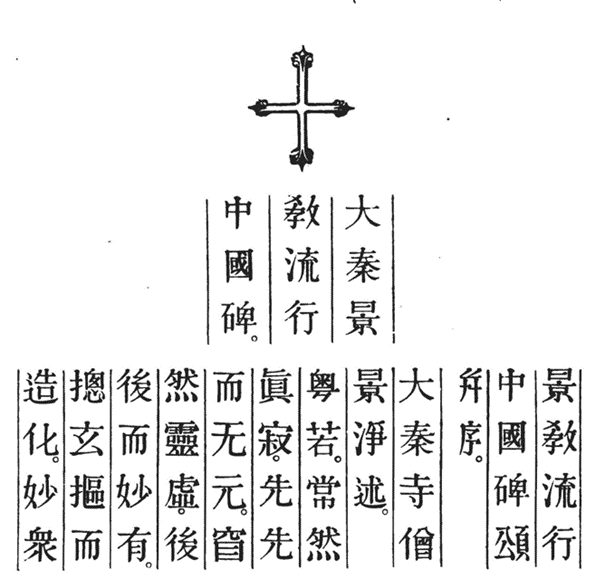
\includegraphics[width=\textwidth]{ChristologieCultureHistoire/Images/PremierParagrapheStele.png}
 
    \label{fig:my_label}
\end{figure}
 Si le livre d'Alopen 150 ans plutôt s'appelait simplement "Sûtra de Jésus-Messiah", le titre de la Stèle est le suivant :
\begin{quote}
    Monument rappelant la propagation à travers l'Empire du Milieu de l'Illustre Religion de Ta-ts'in. \cite{Havret:stelechretienne}
\end{quote}
Ta-ts'in (ou \emph{Da Qin}) indique l'Empire Gréco-Romain. Cette référence peut étonner quand on sait la répugnance des Eglises perses à être trop liées à Byzance. D'ailleurs, traditionnellement, le christianisme en Chine était appelé \textit{Bose Jiao}, l'\textit{enseignement Perse}.  En 745, il prend l'appellation officielle de religion de Da-Qin  possiblement par la chute de l'empire Sassanide perse un siècle plus tôt, qui rend caduque le terme de Perse, l'arrivée d'ambassades byzantines en Chine (attestée en 742) mais aussi par la référence à la philosophie grecque ainsi qu'à l'attribution de voyages en \textit{Da Qin} par le fondateur du Taoisme, Laozi :
\begin{quote}
    Calling Christianity the 'Religion of Da Qin' shows that the Nestorians of the Tang undeniably possessed a sensitive awareness of their political environment within China, and probably internationally as well, and moved with considerable acumen to secure the best possible position for themselves within it (\cite{Barrett:TaoismChristianity})
\end{quote}

\paragraph{Un découpage proposé en 25 sections} La stèle peut être découpée en 25 sections, la première sur les attributs de Dieu, puis les trois suivantes sur la Création et la Chute de l'homme (surtout pour développer l'idée d'un homme bon avant la chute par l'orgueil), puis les deux suivantes sur le Christ. A partir de la section 8, on trouve les caractéristiques de la religion, le baptême, les moines, l'éthique, puis plusieurs sections sur l'histoire des chrétiens en Chine, montrant une loyauté forte vis à vis des autorités politiques chinoises. Nous nous concentrerons sur les premières sections et en particulier les sections 6 et 7 proprement christologiques.  Il faut noter qu'une partie importante est liée à l'histoire du christianisme en Chine et la protection des empereurs. Cette attitude peut être mise en parallèle avec celle des premières communautés chrétiennes, avec Paul, montrant la compatibilité du christianisme avec l'Empire Romain (\cite{Baslez:MondeDevnuChretien}). 






\section{la partie proprement Christologique}

\subsection{Section 6 : l'incarnation} 

La première section qui nous intéresse parle de l'incarnation. Nous indiquerons à chaque fois les deux traductions en Français qui font foi (\cite{Havret:stelechretienne} et \cite{Pauthier:linscriptionSinganfou} \sn{la traduction de Havret est une traduction en latin et français mais la traduction française n'est pas complète - je l'ai complété à partir du texte latin}) :
 
\begin{tabular}{p{0.45\textwidth}p{0.45\textwidth}}
\\
Cependant, notre Trinité s'est comme multipliée, l'illustre et vénérable Messie, voilant et cachant son auguste majesté, se rendant tout semblable aux hommes, est venu en ce monde. les Puissances angéliques publièrent la bonne nouvelle; une femme vierge enfanta le Saint dans la grande Ts'in. Les esprits dans le Ciel annoncèrent la bonne nouvelle : "une Vierge a enfanté le Saint dans la grande Ts'in". Une étoile resplendissante a proclamé la faveur et la Perse, apercevant son éclat, vint lui faire hommage de ses présents. \cite[p. 35]{Havret:stelechretienne} & 

Ce faut alors que notre \textsc{Unité-trine} divisa sa personne dans le resplendissant et vénérable Messie, en voilant sa véritable majesté. il apparut dans le monde comme un simple mortel. Les Esprits dans le ciel annoncèrent la bonne nouvelle : "une Vierge a enfanté le Saint dans la Syrie !"  Une constellation resplendissante a proclamé l'heureux événement; les Perses ayant aperçu sa clarté, sont venus apporter leur tribut. \cite[p. 9]{Pauthier:linscriptionSinganfou} \\
                                                                                  
\end{tabular}
 
 \paragraph{Wo Sanyi, notre "trois-Un". } La pensée Taoiste utilisent le terme de Sanyi :  

\begin{quote} Le terme employé pour désigner la Trinité est un terme taoïste, \emph{sanyi} le "Trois-Un". mais pour signifier qu'il s'agissait de la Trinité Chrétienne, l'auteur de l'inscription a ajusté le caractère "\emph{Wo}" qui signifie "mon/notre". Ainsi le terme taoïste a pris un sens chrétien, "Notre Trois-Un".
    \cite[p.43]{Raguin:JesusMessieXian}
\end{quote}
Quelle est cette trinité taoïste ? Le Trois est pensé comme facteur d'harmonie entre l'Un et le Multiple permettant de «court-circuiter» la référence à Dieu ou à quelque instance supra-cosmique.\cite{Cheng:triadeChinoise}


Le terme utilisé pour le Christ est le terme syriaque de \textit{Messie}, translittéré et non traduit.

 "\textit{Voilant et cachant son auguste majesté, se rendant tout semblable aux hommes, est venu en ce monde}" est quasiment la traduction de Ph 2,6-7, soulignant l'abaissement du Christ.
 

\paragraph{Insistance sur le Ciel et l'environnement}  les cieux (\textit{constellation}) prennent une partie importante dans les deux sections sur le Christ, avec tout un passage sur l'Etoile des mages. On peut  déceler le souhait de l'auteur de montrer ce qu'est le Christ non pas en le décrivant directement comme \textit{forme},  causes ou \textit{logos} mais en insistant sur le \textit{fond},  \textit{le Ciel} qui \textit{ne s'exprime pas}. \cite[p. 109]{PolDroit:voyage} . 
\begin{quote}
    La philosophie gréco-européenne privilégie la « forme » – en grec ancien, \textit{eïdos}. Une « idée » est d’abord une « forme », qui se découpe sur un fond d’espace indifférencié. C’est ce fond d’espace qui retient l’attention chinoise, plutôt que la forme qui s’en détache. Scruter le fond plutôt que les formes, l’indifférencié plutôt que les différences, l’espace plutôt que les choses qui s’y trouvent et s’y découpent, telle pourrait être la première caractéristique de l’attitude chinoise.\cite[pp. 110-111]{PolDroit:voyage}  
\end{quote}
Dès lors, l'attitude des mages perses qui scrutent dans \textit{le Ciel} ce qui change, est finalement celle du sage Chinois. Pour le Taoisme, ce n'est pas par le discours, qui segmente et découpe mais par le biais d'histoires déroutantes, \textit{comme celle de l'étoile des mages}, que l'on peut transmettre la voie. \cite[p. 130-141]{PolDroit:voyage} 
 




\subsection{section 7 : la rédemption } 


Après l'incarnation, le texte développe en plusieurs paragraphes l'action de Jésus : 


\begin{tabular}{p{0.45\textwidth}p{0.45\textwidth}}
\\
Il accomplit les lois anciennes qu'avaient écrites les vingt-quatre Saints, direction des empires dans les conseils. Il fonda la nouvelle religion que la Trine unité, Esprit très pur, n'exprime pas au moyen de paroles, formant à la pratique des vertus par la vraie foi.  & Ainsi, s'est trouvé accompli ce que les vingt-quatre saints avaient annoncée dans l'ancienne loi : " le gouvernement des familles et des États par une grande et suprême doctrine. Il établit la doctrine pure de l'\textsc{unité-trine}, sans l'appeler une nouvelle religion. Il fortifia les bonnes habitudes par l'usage de la vraie foi. \\
\end{tabular}

\paragraph{Jésus est présenté comme un sage} Le texte insiste sur l'Esprit qui soutient la vertu sans passer par une loi (cf Jr 31,33 \sn{Jr 31,33 \textit{Je mettrai ma loi au dedans d'eux, Je l'écrirai dans leur coeur} \newline 2 Co 3,3\textit{Vous êtes manifestement une lettre de Christ, écrite, par notre ministère, non avec de l'encre, mais avec l'Esprit du Dieu vivant, non sur des tables de pierre, mais sur des tables de chair, sur les coeurs.}}  ou encore 2 Co 3,3).

Par cet  \textit{Esprit très pur, qui n'exprime pas au moyen de paroles formant à la pratique des vertus par la vraie foi}, l'auteur propose probablement une théologie accessible à la culture chinoise. pour les Chinois en effet,  ce n'est pas au moyen de raisonnements qu'on atteint le Ciel, qui s'éprouve directement
\cite[p. 117]{PolDroit:voyage} même si notre participation au Ciel en ce monde est parfois voilée.


Cependant, l'auteur ne s'arrête pas à une approche \textit{sans parole} puisqu'il mentionne les \textit{huit béatitudes} : 

\begin{tabular}{p{0.45\textwidth}p{0.45\textwidth}}
\\
Il institua les règles des huit fins, pour purifier les facultés et perfectionner les saints; il ouvrit la porte des trois principes,& Il posa les lois des huit limites morales que l'on ne doit point franchir. la poussière de la terre, purifiée comme le métal dans la fournaise, devint la vérité parfaite. Il enseigna au moindre les trois grandes vertus cardinales; 
\\ 
 en ouvrant les portes la vie et supprimant la mort. & il lui ouvrit les sources de la vie, et anéantit la mort.
\end{tabular}


 \paragraph{Référence à la Bible} Après avoir insisté sur l'éthique de Jésus, l'auteur met l'accent sur le corpus biblique, à la fois dans le registre de l'\textit{accomplissement} de l'Ancien Testament et ses 24 livres/ Saints mentionnés plus haut \sn{hors livres deutérocanoniques} que de l'annonce d'un nouveau Testament\sn{ l'auteur décompte 27 livres alors que le Corpus syriaque ne reconnaissait initialement que 22 livres (l'Apocalypse et les épîtres générales reconnus tardivement) }. 

 \paragraph{Sauver par le registre de la grâce} Face à poussière (Lieu-tch'en), expression bouddhique pour désigner les \textit{souillures de la pureté du coeur},  le texte mentionne les 8 lois morales (Pa-King, "8 circonstances"), comprises comme les Béatitudes (8 béatitudes chez Mt).  Sont aussi mentionnés la porte des trois vertus cardinales (Tch'ang), porte qui ouvre aussi à la vie et supprimant la mort (Mié-se) selon une expression chrétienne traditionnelle. 

Puis suit une expression typiquement bouddhique du soleil lumineux triomphant des porte des enfers (ti-yu) mot à mot \textit{prison de la terre} \cite[p. 49]{Havret:stelechretienne}.  Satan est ici appelé par le terme chinois \textit{Mo}, d'où la traduction de démon :

\begin{tabular}{p{0.45\textwidth}p{0.45\textwidth}}
\\
Il suspendit le soleil lumineux pour triompher de l'empire de ténèbres et {dès lors }les ruses du démons furent toutes pénétrées et déjouées
&  Il suspendit au ciel le brillant soleil de la vérité pour dissiper les habitations des ténèbres; les ruses mensongères du démon furent dès lors pénétrées et déjouées. \\
\end{tabular}



 
 
 

\begin{tabular}{p{0.45\textwidth}p{0.45\textwidth}}
\\
Conduisant à la rame la barque de la miséricorde, il s'éleva aux demeures lumineuses; dès lors quiconque possède une âme a trouvé son salut. L'oeuvre de la toute puissance étant ainsi consommée, il monta en plein midi, homme déifié.& Il mit en mouvement le navire de la miséricorde pour s'élever aux brillantes demeures; les âmes qu'il renfermait purent dès lors, en traversant le fleuve de la vie, obtenir cette fin glorieuse. A l'heure de midi, il s'éleva au séjour de la vérité. \\ Il laissait les vingt-sept livres de l'écriture, où est expliquée la grande réforme pour l'ouverture des \textit{ling-koan}
  \cite[p. 44]{Havret:stelechretienne} & 
Des saints livres ont été laissés au nombre de vingt-sept, qui ont étendu les conversions originelles en libérant les âmes.
  \cite[p. 10]{Pauthier:linscriptionSinganfou} \\
                                                                                  
\end{tabular}
 
  \paragraph{influence bouddhique du mouvement} Avec l'image de la barque de miséricorde (\emph{avalokites 'vara}), nous avons ici une belle image d'origine bouddhique, divinité plus connue en Chine sous le nom de \emph{Koan-yn} et surnommée \emph{Ta-t'se} la grande Miséricorde. D'après le bouddhisme, l'humanité tourne sans cesse comme sur une grande mer jusqu'à ce qu'elle arrive enfin au \textit{nirvana}. 
  
 % -----------------------------------------------
\section{Conséquences en terme de chemin de salut}

Quelles sont les conséquences sur le salut de cette étude rapide des deux paragraphes christologiques ?

\paragraph{Une dimension pratique du salut} Pour les chinois, la dimension pratique des débats est importante : 

\begin{quote}
    Entre ordre confucéen et contestation taoïste, il existe plus de complémentarité, malgré leurs désaccords, que d’opposition frontale. Ne perdant jamais de vue une dimension pratique, les débats chinois sont continûment traversés par des interrogations sur la bonté ou la méchanceté humaine, sur la bienveillance ou la cruauté nécessaire des souverains.

\cite[p. 147]{PolDroit:voyage}  
\end{quote}
 Regardons dans cet esprit le passage sur le mal qui précède les sections sur l'incarnation et la rédemption.
\begin{quote}
   Il arriva que Satan, disséminant ses fraudes, se para de l'ornement emprunté d'une pure essence, et qu'ouvrant une brèche dans cette grandeur morale, au milieu de cet heureux état, il y introduit la ressemblance de la confusion.
De là, des sectes aussi nombreuses que les jours de l'année, qui se suivirent pressées, et tracèrent à la suite leur sillon, tissant à l'envi les filets de leurs lois. les uns, désignant les créatures, s'appuyaient sur elles comme sur leur principe, les autres supprimant la réalité de l'Etre, se plongeaient dans la superstition, d'autres adressèrent des prières et des sacrifices pour attirer le bonheur, d'autres enfin firent parade de vertu pour en imposer aux hommes. 
\end{quote}
 
 
 Le péché introduit par Satan est décrit comme "ressemblance de la confusion". C'est un exemple de l'aspect concret du Chinois :\textit{ Tien-che }. \textit{Tien} signifie un ornement en métal; \textit{che}, chercher à paraître ce que l'on n'est pas ; se parer des dehors. La conséquence sont les \textit{sectes aussi nombreuses que les jours de l'année}; présentant les différentes voies de salut. On y a vu une critique du Taoisme (cette voie est accusé de diviniser les forces de la nature :  \textit{désignant les créatures, s'appuyaient sur elles comme leur principe}) et Bouddhisme aux tendances matérialistes et nihilistes (\textit{supprimant la réalité de l'Etre, se plongeaient dans la superstition}).  
 
 
 
 \paragraph{Par le Baptême, l'Esprit Saint nous éloigne des vaines gloires} Après la partie christologique, l'inscription développe les rites, d'abord le baptême, \textit{quittant les préoccupations vaines et mondaines pour obtenir la pureté}. Ce soucis d'humilité et de quitter le monde  rejoint la pensée du \textit{Chemin} ou \textit{Tao},  
 
 \begin{quote}
     à la fois faiblesse extrême (goutte d’eau) et puissance sans borne (océan). \ldots vent… C’est à force de faiblesse, si l’on ose dire, que le sage parvient à tant de puissance. 
\cite[p. 130 ]{PolDroit:voyage} 
 \end{quote}

Que ce soit dans la partie décrivant la chute ou au moment du baptême (et des vaines gloires), on trouve probablement une description adaptée aux oreilles chinoises, empreintes de la pensée Taoïste.

 Puis, l'auteur décrit la vie monastique : le rôle de la barbe et de la tonsure, images extérieures de la vie intérieure, l'absence d'esclave, l'égale considération de tout homme , le refus des richesses, la pratique de la générosité, le silence et la retenue. A ce titre, ils se présentent moins comme des moines bouddhiques que comme des sages pétris de sagesse confucéenne : 
 
 \begin{quote}
     Car le « mandat du Ciel », comme disent les confucéens, est présent avant tout dans le « sens de l’humanité » (ren) qui habite le cœur de chacun. Cette notion fondatrice, malaisée à définir, implique à fois, selon Confucius, d’être « juste dans le jugement », « conscient de la valeur de l’effort », « pacifique dans les conflits » et d’avoir de la « retenue ». Le \textit{ren} est ainsi l’instance de régulation des rapports entre les humains, agissant au cas par cas.

\cite[p. 122]{PolDroit:voyage}  
 \end{quote}
 Paul a préféré  l'aréopage au Temple, et les apologistes Chrétiens le terme néo-platonicien de  \textit{Logos} pour dire l'expérience du Christ et non les catégories des religions paiennes. De même, l'auteur de la \textit{Stèle} nous semble mettre en avant la sagesse confucéenne, plutôt que les moines Taoistes ou bouddhistes. Cette attention à la sagesse confucéenne explique peut être  la mention qui suit : les moines prient \textit{au secours des vivants et des défunts}, alors que la sagesse confucéenne accorde une importance forte au culte des ancêtres.
 
 

 
 
  
\paragraph{Ne pas penser séparément morale, rites privés et gestion des affaires communes} Une caractéristique importante de la civilisation chinoise est effet d’entrelacer doctrines morales, rites privés et gestion des affaires communes
\cite[p. 120]{PolDroit:voyage}. L'inscription développe non donc seulement le credo de la foi chrétienne (sections 7 et 8), mais aussi la morale et les rites (sections 9 et 10). A ces deux éléments s'ajoute la louange des empereurs chinois. Sur ce dernier point, les Chrétiens en Chine reprennent  la stratégie des chrétiens face à l'empire romain, qui s'inséraient dans le réseau de solidarité des villes par le rôle des évêques et des diacres (\cite{Baslez:MondeDevnuChretien}).


\section{Conclusion}

\paragraph{Une présentation du message Chrétien soulignant les aspects les plus accessibles à la pensée Chinoise} A travers l'étude de la Stèle, nous avons trouvé la présentation des principaux points de la Foi Chrétienne. Cependant, sans trahir le message chrétiens, l'auteur choisit une traduction qui résonne avec la culture chinoise. Au delà de la traduction, le choix des passages de la Bible comme \textit{l'Etoile dans le Ciel} ou l'accent sur certains points du rite comme la prière pour les défunts ou l'attention au \textit{Ren}, éclaire ce message chrétien de façon nouvelle. 
 
\paragraph{difficulté à penser l'acculturation religieuse} Dans nos recherches, nous avons rencontré des auteurs ne pouvant pas penser l'acculturation du message chrétien en dehors des catégories de l'hérésie. Ainsi, un article récent \cite{Gernet:Stele} s'oppose à l'interprétation d'une stèle de Xi'an acculturée à la culture chinoise et propose une clé de lecture basée sur un contexte de luttes théologiques internes au sein de l'Église nestorienne.

\begin{quote}
    rien ne prouve d'ailleurs clairement que les nestoriens aient songé à faire partager leurs croyances aux Chinois. [\ldots] Les circonstances et les mentalités étaient en effet tout à fait différentes de celle qui devait régner un millénaire plus tard, à l'époque de la contre-Réforme animée par une ambition de conquête universelle des esprits et des territoires (p. 245)
\end{quote}
Même si la communauté chrétienne qui a écrit la stèle était toujours fortement liée à l'Église perse - comme le montre les signatures de la stèle en araméen -, cette thèse nous parait difficilement acceptable à l'analyse. Les Eglises syriaques à cette époques nous sont certes assez mal connues; on peut noter l'importance du terreau judeo-chrétien à la création de ces Eglises, le milieu missionnaire parmi les marchands, la mixité culturelle, reflet des sociétés en monde iranien, la loyauté vis à vis des autorités politiques et le monachisme (\cite{Amir:CoranHistoriens}). Sans les relever tous, on retrouve de fait de nombreux éléments syriaque dans la Stèle (par exemple, influence des marchands et moines dans la création de l'Eglise de Chine), mais sans que cela ne remette en question le travail d'acculturation de la foi chrétienne en contexte chinois dont les marques sont soulignées par de nombreux sinologues. A tel point que c'est plutôt l'autre vision, celle d'une supposée trop grande acculturation qui est souvent soulignée (le P. Havret, sj note par exemple les 
\textit{    dangereux rapprochements} avec la culture Taoiste \cite[p.21]{Havret:stelechretienne}).   


Cette double polémique montre la difficulté à penser l'acculturation et sa conséquence en terme de christologie : notre vision du Christ est forcément transformée par l'acculturation, et elle peut être vécue sans être un dévoiement de la foi véritable, mais au contraire en développant des aspects du Christ qui sont restés comme en germe dans son incarnation en Judée "au temps d'Hérode" et qui peuvent se développer pleinement dans d'autres cultures et époques. 

%\chapter{Evolution de l'interdiction du \riba et Gharar}


a. Un dossier sur un thème lié au cours A partir de trois articles universitaires minimum. -  Introduction : intérêt du thème au regard de l’actualité et/ou de vos propres orientations personnelles ; présentation des articles et de leurs auteurs. Présentation du plan de votre travail. - Synthèse (ne pas présenter les articles séparément mais faire une synthèse à partir des différentes thématiques rencontrées) - Contextualisation de ce thème dans l’islam contemporain, éclairage par le contenu du cours (enjeux, dynamiques, etc). 

\section{Introduction}

En tant que membre du jury de l'Institut des Actuaires, j'ai eu à me prononcer sur certains mémoires présentés par des étudiants sur la \textit{finance Islamique} et \textit{l'assurance Takaful}. Ces mémoires ne couvrent pas les présupposés théologiques et commencent généralement par une présentation des interdits de la loi musulmane, comme par exemple ce \href{http://www.ressources-actuarielles.net/EXT/ISFA/1226-02.nsf/0/8c814ff5f2bae57ec1257e1a004407b6/\%24FILE/Memoire_ISFA_Tontines_et_Takaful_Bendimerad_Version_avec_Couverture.pdf}{mémoire d'actuariat} : 
\begin{quote}
     [pour faire face à ses  engagements, l'assureur],peut, par exemple, inclure des actifs obligataires dont les taux de rendement font apparaître des taux d'intérêt. [...] l'interdiction de l'usage du taux d'intérêt, appelé \textit{\riba} en arabe, est l'un des fondements du droit des affaires musulman.
\end{quote}
Dans la même veine, sont généralement définis les autres interdits, comme le \emph{Gharar}, défini dans le même mémoire comme : 
\begin{quote}
    Le contrat d'assurance peut constituer une perte disproportionnée en faveur de l'un des participants aux dépens de l'autre. Ce caractère d'incertitude, appelé \textit{Gharar} en arabe, est un caractère prohibé par l'Islam surtout lorsque le transfert du risque vers un tiers est total, ce qui est notamment le cas pour l'assureur qui porte entièrement la charge du risque cédé par l'assuré.
\end{quote}
Les mémoires d'actuariat consultés essayent de dépasser ces interdictions, qui soulignent une tension avec les \textit{Hadiths} : 

\begin{quote}
     
A l'issue de l'analyse précédente, l'idée même d'une assurance islamique semble être un contresens. Pourtant, la religion musulmane encourage l'individu à prendre des mesures pour réduire l'ampleur des désastres qui pourraient l'affecter. D'après un Hadith authentifié, le prophète conseille à un croyant de placer sa confiance en Dieu et d'attacher son chameau plutôt que de se limiter uniquement à placer sa confiance en Dieu en offrant la possibilité au chameau libre de s'échapper. L'Islam ne s'oppose donc pas à l'idée de vouloir minimiser les risques et par conséquent elle ne s'oppose pas à faire usage de la loi des grands nombres. Elle exclut certes la spéculation et l'incertitude ainsi que le taux d'intérêt. En revanche, elle compte parmi ses principes la coopération et l'entre-aide mutuelle ainsi que le partage équitable des risques et des bénéfices. Toutes ces bases ont permis de concevoir un modèle alternatif à celui de l'assurance conventionnelle.
\end{quote}
De cette tension naît des solutions techniquement assez complexes.


Intrigué par cette apparente clarté vis à vis de l'interdiction de l'\textit{intérêt} et de l'\textit{l'incertitude} à la base de l'économie moderne, je me propose d'étudier l'évolution de l'opposition de la \emph{\riba} et \emph{gharar} dans les différents courants de l'Islam contemporain, depuis la pensée d'Abduh jusqu'aux frères musulmans et le salafisme. 
L'interdiction des deux notions n'a pas la même importance économique et la \textit{\riba} a donné lieu à plus de développement. En partant de ces études, j'essayerais néanmoins de transposer ces travaux à l'assurance.
Après avoir regardé  à travers l'étude de ces deux notions comment l'économie moderne, pensée au XVIIIè et XIXè siècle questionne l'Islam, je poserai quelques pistes sur le propre questionnement du Christianisme. Après tout, le prêt à intérêt était aussi interdit au Moyen-äge en Europe (Concile de TOurs de 1163). Ces pistes seront en particulier nourries par l'étude de la pensée de Saint Thomas d'Aquin sur les taux d'intérêt et comment ces pistes peuvent nourrir la réflexion de la théologie musulmane (et chrétienne) contemporaine. 
 

%---------------------------------------------------------------------------------------------------------------
\section{Vision dans l'Islam Classique de l'interdiction de \riba}

\subsection{une interdiction de la \riba et Gharar}

Pour commencer, il est utile de se référer aux textes à l'origine de ces interdits.
\paragraph{Versets du Coran et Hadiths interdisant la \riba}
Le verset 130 de la Sourate 3, Al-Imran mentionne : 
\vocalize % switch diacritics for short vowels on
\transtrue % display the transliteration
\arabtrue % print arabic text (on by default)
\begin{quote}
 
\TArabe{
 يَا أَيُّهَا الَّذِينَ آمَنُوا لَا تَأْكُلُوا الرِّبَا أَضْعَافًا مُّضَاعَفَةً وَاتَّقُوا اللَّهَ لَعَلَّكُمْ تُفْلِحُونَ
  } 
   [3,125] O vous qui croyez !, ne vivez pas de la \textit{\riba} [produisant le] double deux fois ! Soyez pieux envers Allah ! Peut-être serez-vous bienheureux. 

\end{quote}
\begin{quote}
\TArabe{278
 يَا أَيُّهَا الَّذِينَ آمَنُوا اتَّقُوا اللَّهَ وَذَرُوا مَا بَقِيَ مِنَ الرِّبَا إِن كُنتُم مُّؤْمِنِينَ
279 فَإِن لَّمْ تَفْعَلُوا فَأْذَنُوا بِحَرْبٍ مِّنَ اللَّهِ وَرَسُولِهِ وَإِن تُبْتُمْ فَلَكُمْ رُءُوسُ أَمْوَالِكُمْ لَا تَظْلِمُونَ وَلَا تُظْلَمُونَ
} 
 [2, 278] O vous qui croyez !, soyez pieux envers Allah ! Faites abandon de ce qui [vous] reste [à toucher provenant] de la \textit{\riba}, si vous êtes croyants !
[2, 279] Si vous ne le faites point, attendez-vous à une guerre de la part d’Allah et de Son Apôtre ! si vous vous repentez, alors vous récolterez votre capital sans infliger ou être victime d’une injustice. \sn{Traduction de Blachière, sauf la dernière phrase \cite{ElGamal:BanqueFinanceIslamique}}

\end{quote}

De même, un hadith de Abu Hurayra met au même niveau la \textit{\riba} et le meurtre : 
\begin{quote}
    "Evitez les sept turpitudes !"

- "Quelles sont-elles, ô Envoyé d'Allah?", demandèrent les fidèles.


- "Ce sont, répondit-il :

 

-le polythéisme,

-la magie,

-le meurtre qu'Allah a interdit sauf à bon droit

-l'usurpation des biens de l'orphelin,

-la \textit{\riba},

-la fuite du front au jour du djihad et

-la fausse accusation (de fornication) des femmes vertueuses, chastes et croyantes".
\end{quote}
 
  Nous avons évité à ce stade de traduire le terme de \textit{\riba}, par \textit{usure} ou \textit{intérêt}. Le Hadith rapport par at-Tirmidhî a été utilisé pour appliquer le sens d'intérêt à la \textit{\riba}  : 
 \begin{quote}
     Vendez de l'or contre de l'argent (les quantités échangées étant) comme vous voulez, à condition que ce soit main à main. Vendez du blé contre des dattes sèches (les quantités échangées étant) comme vous voulez, à condition que ce soit main à main. Vendez de l'orge contre des dattes sèches (les quantités échangées étant) comme vous voulez, à condition que ce soit main à main (n° 1240)
 \end{quote}  
 On peut effectivement y lire le refus de l'intérêt mais d'autres lectures sont possibles, en particulier en relevant l'insistance du hadith à une transaction \textit{main à main}, qui permet une transaction claire. Par ailleurs, la valeur du temps n'est pas explicitement mentionnée.
 

 
\subsection{un nouveau contexte avec la naissance du Capitalisme}
Du point de vue du prêteur, le prêt à un prix du fait du risque  que l'emprunteur repaye le prêt, la valeur temps (qui correspond à l'inflation et à la perte d'opportunité d'un investissement aujourd'hui qui rapporte plus plus tard). La pertinence économique de l'intérêt et de la prise de risque est donc justifiée même si cela ne veut pas dire qu'elle l'est d'un point de vue religieux.
Avec l'accumulation des richesses dans les villes italiennes au moyen-âge naît le capitalisme et la finance : comment financer et assurer les bateaux partant de Gênes et remplis de richesse ? Cette irruption de la finance pose de nouvelles questions.  Face à cette accumulation, une réponse théologique chrétienne sera la création de l'ordre mineur par Saint François d'Assise. Et, nous reviendrons sur ses développements, la réflexion de l'université de Paris et de Saint Thomas d'Aquin sur la notion d'usure et de juste prix.  
Ces innovations touchèrent tardivement le monde musulman, au XIXème, avec l'arrivée simultanée de l'industrialisation, qui nécessite des capitaux importants et les débuts de la colonisation. Par l'industrialisation, la capacité productive est fortement augmentée par l'investissement, mais aussi la concentration des risques qui ne peuvent être portée par la solidarité traditionnelle.
Face à cette nouvelle question, quelles sont les réponses proposées par les théologiens musulmans depuis l'arrivée de cette question ?


%---------------------------------------------------------------------------------------------------------------
\section{Elements théologiques apportés}

\subsection{Premières réponses face à la nécessité du prêt}
\paragraph{Le développement du \riba et de l'assurance par les Occidentaux} Les prêts à intérêt ont toujours existé au sein de l'Empire Ottoman\cite{Gilbar:Qadi}, et proposés par des familles grecques, arméniennes ou Juives (et en Iran par les arméniens et zoroastriens). A ce premier Groupe, s'ajouta les banques commerciales européennes ou les banques "étrangères-locales" comme la banque impériale ottomane au XIX.
De la même façon pour les assurances, Ibn Abidin, représentant de l'école officielle de droit Hanadi dans l'empire ottoman, suggère le compromis suivant : il est licite d'établir ds contrats d'assurance portant sur les risques encourus à l'intérieur du royaume islamique - le Dar al Islam -à condition que ces contrats soient conclus avec une compagnie d'assurance ayant son siège hors de pays de l'Islam. 

\paragraph{Utilisation de prêt à intérêt par les musulmans malgré l'interdiction du \textit{\riba}.} La \textit{\riba} a pu poser des problèmes dans son implémentation, en particulier pour les grands marchands (tujjār).  
Pour l'école Hanafite, le terme de \riba peut être traduit par usure, dans le sens d'un taux d'intérêt exhorbitant, à l'opposé de l'intérêt raisonnable, le \emph{ribh}. L'autre interprétation dominante, attribuée à 'Abdahallah Ibn 'Abbas, permet d'expliquer la notion du Coran de double capital par la pratique du \textit{\riba al jâhiliyya} (préislamique), avec des taux d'intérêt très élevés avec des intérêts pouvant dépasser le capital en cas de non-paiement. A l'opposé de ces analyses plus ouvertes, la position de l'école Hanbalite fut l'interdiction pure de l'intérêt. Pour contourner l'interdit du \riba face à la nécessité, les marchands musulmans mirent en place des montages complexes où l'intérêt était déguisé en une \textit{double vente} (\emph{mukhâtra}) avec deux ventes fictives successives permises par la \textit{sha'ia}: 
\begin{itemize}
    \item la première, le préteur vent un objet à l'emprunteur pour une somme équivalente au capital et à l'intérêt. l'emprunteur s'engage à payer la valeur de l'objet à la fin de la période (techniquement, une vente avec paiement différé). 
    \item A la fin de cette première transaction, l'emprunteur revend le même objet pour la valeur du principal (techniquement, une vente à terme).
\end{itemize}
 Cependant, l'étude des jugements des cours religieuses au moyen-orient entre le XVI et le XVIII montre que malgré ces montages, des exemptions partielles ou totales de paiement de l'intérêt du fait de son incompatibilité avec l'Islam \sn{GILBAR, GAD G. “The Qadi, the Big Merchant and Forbidden Interst (Ribā).” British Journal of Middle Eastern Studies, vol. 39, no. 1, 2012, pp. 115–36, http://www.jstor.org/stable/23264404. Accessed 3 May 2022.}
 

\section{la pensée d'Abduh et Rida}
\subsection{position d'Abduh} Le Cheikh {Muhammad Abduh} (1849 - 1905) Egyptien, successeur d'Al Afghani, est la figure marquante du réformisme islamique. Il s'oppose au colonialisme atteignant alors l'Egypte. Son séjour  parisien le convainc de la nécessité de réforme de l'Islam et l'initie aux réflexions intellectuelles occidentales et en particulier François Guizot. A sa suite, il il pense l'Islam comme civilisation et pas uniquement comme Religion, avec la notion de progrès lié à la civilisation. Il n'y a pas d'opposition pour lui entre Foi et Raison, la religion musulmane étant \textit{raisonnable}.    Dans son livre \citet{Abdou:Rissalat}, il part de la Raison pour montrer le besoin que l'homme ne se fixe pas sa propre loi.

Il montre tout d'abord la naissance des besoins et des liens entre les hommes. Idéalement ces liens seraient ceux de l'amour : 
\begin{quote}
    Nul ne met en doute que chaque membre d'une société a besoin
des autres membres; et chaque fois que l'individu accroître ses exigences
dans la vie il ressent plus fortement le besoin de recourir au concours
de ses semblables. Ainsi se développent les besoins et à leur suite s'étendent
les relations de la famille à la tribu, de celle-ci à la nation, et finalement
au genre humain tout entier, comme le montre notre époque . Ces
besoins qui créent dans le sein de chaque nation (surtout dans le sein de
celles qui méritent vraiment ce nom) des relations et des rapports
spéciaux la distinguant des autres nations, sont le besoin de se procurer
sa subsistance, celui de profiter des biens de la vie, celui d' acquérir
les choses désirables et d'éloigner de soi celles qui déplaisent. 
Si la vie de l'homme se déroulait selon les lois de la nature, telles
que nous les voyons appliquées aux autres êtres vivants, les besoins
que nous venons de citer auraient été parmi les facteurs les plus puissants
de l'amour entre les individus[...].  

[\ldots]
Si par contre, l'intérêt se mêle aux relations amicales, et si chacun des amis exige un prix pour son amour, celui-ce se change en esprit d'exploitation, il se reporte sur l'effet utilitaire et se transforme chez l'un des amis en un abus de la force, et chez l'autre, en peur avilissante, en dissimulation et en hypocrisie.
\cite[p.66]{Abdou:Rissalat}
\end{quote}
Mais l'homme ne vient pas selon les lois de la nature car il est inconstant : 
\begin{quote}
 l 'homme
a été créé avec un caractère inconstant; quand le malheur l'atteint
il est abattu, et quand il acquiert quelque bien il devient insolent.
(C. ch. 70, v. 19 à 21). [...]
Chaque fois que la mémoire et l'imagination les poussent à
éviter quelque chose qui leur inspire de la crainte ou à atteindre un
objet qui leur fait envie, leur intelligence leur ouvre une porte de la
ruse ou leur découvre une voie de la violence ; alors le rapt remplace
l'échange pacifique, la dispute prend la place de l'union et la conduite
de l'homme riche s 'appuie plus que sur l'astuce et la violence.
\cite[p 68]{Abdou:Rissalat}
\end{quote}
il montre qu'on peut accéder à l'équité par des voies naturelles mais qu'à la foi pour les masses et pour éviter la corruption des élites, il est nécessaire de s'appuyer sur loi externe.
\begin{quote}
[...] ] le genre humain
a surtout besoin, pour conserver son existence, de l'amour ou d'un
sentiment qui le remplace.
A différentes époques il y a eu des penseurs qui ont fait appel à
l'équité ; ils ont pensé, et même quelques mystiques ont exprimé cette
pensée par de nobles paroles, que l'équité remplace l'amour. Cette
assertion ne manque pas de sagesse, mais qui est-ce qui peut établir les
règles de l'équité et amener la totalité des hommes à se soumettre ?
\cite[p 69]{Abdou:Rissalat}
\end{quote}

Suivre la Loi de Dieu, ordonner le bien est alors supérieur à la foi : 

\begin{quote}
  le Coran indique
qu'il n'y a pas de condition meilleure que celle des hommes qui ordonnent
le bien et défendent le mal: \begin{quote}
    Vous êtes les meilleurs parmi les hommes,
vous ordonnez le bien, vous défendez le mal et vous croyez en Dieu. (Cor. ch. 3, v. 106.) 
\end{quote} 
 
Dans ce verset le fait d'ordonner le bien et de
défendre le mal est mentionné avant la foi en Dieu, bien que la foi soit la base même sur laquelle s'appuient les bonnes oeuvres. 
\cite[p 121]{Abdou:Rissalat}
\end{quote}

\paragraph{Conséquence pratique pour la \riba}
'Abduh liste alors une liste de maux que l'Islam permet d'éviter : 
\begin{quote}

[l'Islam] nous invite par dessus tout à dépenser notre bien pour les oeuvres
charitables et souvent il en fait l'expression de la foi et la manifestation
d'une bonne conduite; il déracina par là, du coeur des pauvres, la rancune
et la haine contre ceux que Dieu a favorisé des biens terrestres ; il leur
inspira l'amour pour les riches, tout comme il fît naître dans le coeur de
ceux-ci la pitié pour les malheureux ; ainsi il développa la confiance dans
le coeur de tous les hommes. Quel remède plus efficace contre les maux
dont souffre la société: « C'est une faveur que Dieu accorde à qui il veut,
car Dieu est d'une bienfaisance sans bornes. » (Cor. ch. 57, v. 21.)
\textbf{L' Islam a fermé les deux portes du mal, il a bouché les deux sources
qui minent l'intelligence et détruisent la richesse, en frappant les boissons
enivrantes, les Jeux de hasard et l'usure, d'une interdiction absolue qui
n'admet pas d'infraction.}
\cite[p 122]{Abdou:Rissalat}
\end{quote}
Ainsi, parmi ces maux figure la \riba traduit ici par \textit{usure}.

\paragraph{Pratiquement : l'avis d'Abduh sur l'ouverture de la Caisse d'Epargne en Egypte}
L'ouverture de la Caisse d'Epargne et la répugnance d'un certain nombre de musulmans à toucher les intérêts poussèrent la caisse d'épargne à demander à 1903 une Fatwa à Abduh \cite{Jomier:AdbouCaisseEpargne}. Cette fatwa semble n'avoir jamais existé. En revanche, Ce fut à la requête d'un particulier mais en fait pour la
Compagnie d'Assurances sur la vie Gresham. La Compagnie d'Assurances al-Chark,
au Caire,  conservait une copie d'une fatwa d'Abduh \textit{écrite initialement pour un particulier} afin de la montrer à ses clients, le cas échéant. Le
client effectue des versements réguliers et périodiques par tranches successives
prévues d'avance ; la compagnie les encaisse et se charge de faire fructifier cet
argent. Finalement, à l'échéance, la société remboursera le total des versements
effectués augmenté des bénéfices résultant de la fructification. La fatwa admet
la licéité d'une telle opération en des termes qui, au fond, s'appliqueraient à toute
société en commandite. Il faut noter que la revue Al-Manâr de \textit{Rashid Rida} ne nia pas l'authenticité de cette fatwa après la mort d'Abduh mais protesta contre l'extension faite à toute assurance vie.

\paragraph{la note de la revue Al-Manâr de 1903}


Face aux scrupules de 3000 musulmans à toucher les intérêts (fa'ida), un échange eu lieu entre le directeur de la Caise d'Epargne et Abduh, échange repris par la revue \textit{Al-Manâr}. Abduh y maintenait fermement le principe de
l'interdiction absolue de l'usure (al-ribâ) ; mais il ne classait pas le cas de la Caisse
d'Epargne avec ceux de l'usure. Il l'assimilait à celui d'une société en commandite
(chirkat al-mod'âraba). A la suite de cette discussion, la loi fut modifiée en 1904 : 
 

\begin{quote}
 Il est prévu dans l'article premier que le client devra signer un
formulaire imprimé dans lequel il déclarera donner au Directeur Général de la
Poste tout pouvoir pour faire fructifier les sommes déposées, d'une façon licite et
en excluant toute opération usuraire. Il déclare permettre au Directeur de la Poste
de joindre ses dépôts à ceux des autres clients pour les faire fructifier en commun
à condition de recevoir une part de bénéfices (al-ribh') proportionnelle à ses
versements. On notera que dans cet article comme dans tout le reste de la loi le
mot de \textit{fâ'ida}, intérêt, est totalement absent. \cite{Jomier:AdbouCaisseEpargne}
\end{quote}

\begin{quote}
    L'article deux stipule entre autres ce qui suit. Il évite de parler de tant pour
cent, formule qui rappelle trop les intérêts. Il note que la part des bénéfices ne
dépassera pas un pour quarante du capital et le surplus, s'il y en a, reviendra à
l'administration postale à titre de compensation pour les services rendus et les
frais que ceux-ci comportent. L'assimilation à la société en commandite est ainsi
mise en accord avec le fait que la proportion des bénéfices touchés est fixe. On
notera que la proportion de un pour quarante est familière aux oreilles des
musulmans pieux puisque dans un certain nombre de cas le montant de la Zakat
atteint ce chiffre.
\end{quote}

On voit donc la position d'Abduh comme ferme dans les principes et ouvert dans l'application, même si cela se traduit par une subtilité juridique.


% - ----------------------------------------
\subsection{L'approche de Rashid Rida sur la \riba} 

Rida est l'un des successeurs spirituels de Abduh. Il fonda avec Abduh la revue néo-réformiste al-Manâr en   1898. Elle définit sa politique éditoriale à l’égard « de la civilisation occidentale » sous forme de deux impératifs : 
\begin{quote}
    \item  1/ Il faut que la terre musulmane puisse rattraper l’Europe sur le plan des sciences modernes, de l’industrie et de l’innovation technique. 
    \textbf{ }2/ En contrepartie, il faut déclarer une guerre sans merci à tout ce qui a accompagné l’entrée des Européens en terre musulmane comme décadence morale et mauvaises mœurs
\end{quote}

\paragraph{Une lecture de la \riba originale à la base de l'économie Islamique } face au développement des banques avec intérêt dans tous les pays colonisés et particulièrement en Egypte, il est important pour Rida de refonder les principes sous-jacents à l'intérêt et à l'économie financière \cite{Siddique:DemystifyingRiba}. Face à des lectures libérales (\riba comme usure) et à l'opposé, les musulmans socialistes (\riba comme profit), il existe une position médiane mais qui mérite d'être précisé : 


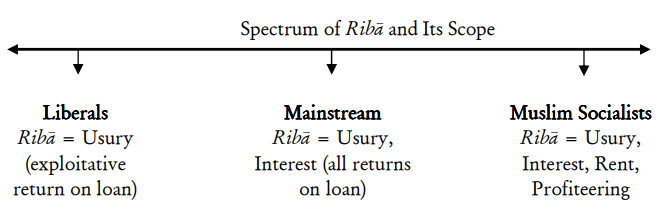
\includegraphics[width=0.9\textwidth]{CourantsIslamContemporain/ImagesCourantsIslamContemporain/Riba.png}

Rida part de l'analyse du mot \riba comme \textit{excès}, et en particulier reprend l'analyse de Co 3,125 présentée au début d'un excès lié à la renégociation de la dette. De là, il conclut que ce qui est interdit par le Coran sont les intérêts ajoutés à la fin de la période de prêt (\riba ’l-jahiliyyah). D'une certaine façon, ce sont les intérêts composés qui sont interdits, le fait que les intérêts augmentent en cas de non paiement. Cela lui permet d'autoriser les intérêts bancaires :
\begin{itemize}
    \item ils ne doublent pas les taux
    \item l'ajout d'un intérêt fait partie du principal de la même façon que le prix d'une vente à crédit (\emph{\riba al-buyu}) qui ne sépare pas principal et intérêt et qui est autorisé par le Coran.
\end{itemize}
 Il fait une distinction entre la \riba interdite dans le Coran et celle des Hadiths (voir graphique \ref{fig:MinorityRiba}) :

 \begin{figure}[h!]
     \centering
     \sidecaption{\cite{Siddique:DemystifyingRiba}, une séparation entre Coran et Hadith}
      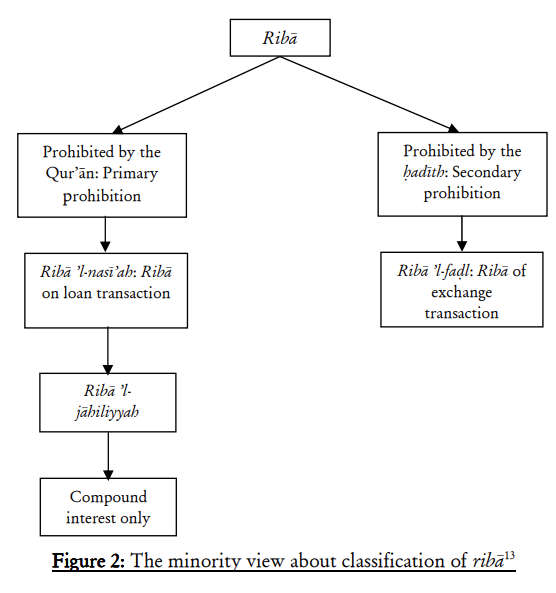
\includegraphics[width=0.5\textwidth]{CourantsIslamContemporain/ImagesCourantsIslamContemporain/RibaRida.png}
      \caption{La présentation du Riba selon Rida, dite minoritaire}
     \label{fig:MinorityRiba}
 \end{figure}
 
 Rida ne sera pas suivi par une majorités de jurisconsultes sur la légitimité des taux d'intérêt. En revanche, ils adopterons sa distinction entre less différents \riba, en étendant l'interdiction de la \riba du Coran à tout intérêt et pas seulement intérêt d'intérêt. Mais du coup, se pose la question du Hadith : pourquoi interdit-il  la \rib \emph{Al-Fadl}, c'est à dire la di
 
 

 
\paragraph{Les frères musulmans}
Dans les perspectives du réformisme musulman,
cette question d'ailleurs est loin d'être insoluble car une société qui émet des
actions peut être assimilée à une société en commandite. Les dividendes
représentent alors la part des bénéfices proportionnelle au capital engagé... 
al-Banna, fondateur des Frères Musulmans en Egypte, avait admis la licéité de ce
genre d'opérations et des Frères avaient, peu avant 1 948, fondé quelques ateliers
ou sociétés financées par ce procédé (2). La difficulté principale vient de ce que la
langue arabe n'a pas de mot spécial pour désigner les dividendes et que le terme
fâ'ida a des relents de ribâ.
\begin{quote}
    III. 2 interdiction de pratiquer l'usure, orienter les banques vers cette interdiction, le gouvernement doit donner l'exemple en abandonnant l'\textit{intérêt} fixé par les banque du prêt et du prêt industriel, etc. \textit{programme des frères Musulmans, 1936}
\end{quote}
%---------------------------------------------------------------------------------------------------------------
\section{Naissance de la finance et de l'assurance Islamique}

\subsection{Ce que l'on voit : Malaisie,...} 

\paragraph{une pratique supposant une \textit{shari'ah} qu'on ne peut interroger}

\subsection{Quelle est la théologie sous-jacente}

\paragraph{Une évolution de la shari'a par les principes} Mohammed Talbi 
\begin{quote}
    Il existe
trois principes en islam permettant de faire évoluer le droit et de
l'adapter
à la réalité, 

la \emph{maslaha} c'est-à-dire l'utilité publique, un
concept qui date du II\textsuperscript{e} siècle de l'hégire, 

la
\emph{zharoura}, la nécessité, c'est un principe fort puisqu'il est dit
que "la nécessité rend permis l'interdit" ; 

et les \emph{maqassid}, les
finalités de la loi. 

\begin{Synthesis}
On part des principes contre les principes. 
\end{Synthesis}
\sn{voir p. \pageref{TroisPrincipesEvolutionsShari}}
\end{quote}


\section{Conclusion}

\paragraph{une variété importante de vision mais toujours basée sur la sharia}

\paragraph{une réflexion sur la base de la Sharia'}
voir ce que Candiard dit de ce théologien qui dit de ne pas faire de Kalam mais du droit.

\paragraph{quel pourrait être les pistes de Kalam, quelques pistes de l'expérience occidentale ?}

\paragraph{St Thomas et l'usure : une réflexion autonome de la théologie}

\paragraph{extension du juste prix dans les risques : la dimension actuarielle}
\paragraph{Au XIXème, réflexion neo-thomiste et patristique pour sortir du carcan}
Après avoir regardé comment l'économie moderne, pensée au XVIIIème et XIXème questionne l'Islam à travers l'étude des différents courants de l'Islam contemporain, je poserai quelques pistes sur le propre questionnement du Christianisme. Après tout, le prêt à intérêt était aussi interdit au Moyen-äge en Europe. Ces pistes seront en particulier nourrie par l'étude de la pensée de Saint Thomas d'Aquin sur les taux d'intérêt et comment ces pistes peuvent nourrir la réflexion de la théologie musulmane. 

Nous catholiques au XIX par rapport à la modernité: renouveau thomiste et patristique. Liberté de pensée par rapport aux questions de l’époque
« A quoi on tient en vrai »
Le raccourci de certains théologiens musulmans : faire le court circuit pour repenser les choses : obsession juridique. Comment on sort du droit ? En faisant de la théologie. Et pour cela retour à la tradition
Voile
Le coran la dit donc il faut se voiler. Voile : hijab n’est pas dans le coran. Rideau
Zina : qu’il faut cacher
Jilbab pour les filles et femmes du prophète 
Ibn el jahouzi : voile non mentionné. Dimension non religieuse

Des écrits au XX. Deux raisons : les femmes vont occuper plus de rôle dans l’espace publique.
Et renouveau de l’anti théologie. Le voile est une question de théologie. Question de la foi
	⁃	Saint Paul : la foi et les œuvres
	⁃	On comprend croyant non pratiquant
	
%\chapter{Matériaux bruts pour validation}

\section{A lire}
\href{https://www.persee.fr/doc/ridc_0035-3337\_1955\_num\_7\_3\_9521}{Le prêt à intérêt et l'usure au regard des législations antiques, de la morale catholique, du droit moderne et de la loi islamique }

\section{Refus de l'intérêt en milieu chrétien}

\subsection{1163 : le concile de Tours condamne le prêt à intérêt}


Le 01 septembre 2014

La condamnation du prêt à intérêt par l'Eglise n'a pas empêché, au travers de divers subterfuges, le développement du crédit, moteur de l'activité économique.

Dans l’Occident chrétien médiéval, le rôle de prêteur sur gages, souvent pour de faibles montants, sera longtemps assuré par des juifs, que leur religion autorise à prêter avec intérêt à des non-juifs. Mais dès le XIe siècle, de nombreux bourgeois chrétiens enrichis se livrent au prêt à une autre échelle. Déjà au XIIe siècle, des bourgeois d’Arras, de Cahors, des Lombards d’Asti, des Génois prospèrent par ces opérations.

Certes, l’Eglise et les princes qui se conforment à sa loi bannissent le prêt à intérêt en s’appuyant - entre autres - sur l’Evangile de Luc : "Prêtez-vous l’un à l’autre sans rien en attendre." En France, le concile de Tours de 1163 condamne une des formes du prêt à intérêt dans le cadre de la moralisation de l’Eglise : nul clerc (évêque, abbé) ne peut désormais prêter de l’argent et recevoir en gage un

\section{Extrait site internet}
\begin{quote}
En Islam, le Riba est interdit : il s’agit de l’un des plus grands péchés, qui tire son origine du Coran. Mais il est également l’un des plus banalisés. Le Riba, appelé « usure », désigne l’intérêt perçu sur de l’argent prêté. De nos jours, le Riba est partout présent dans le domaine financier, à savoir, dans les comptes d’épargne, dans les prêts à intérêts, dans les agios… Alors, qu’est-ce que le Riba exactement ? Pourquoi est-il interdit ? Comment financer vos projets sans Riba 
\paragraph{Définition du Riba}

Le Riba peut être défini par intérêt - usure. Si le terme « usure » est la traduction la plus fréquemment donnée à cette interdiction de l’intérêt usuraire, il est important de préciser que le mot Ribâ vient cependant du verbe rabâ \& arbâ qui signifie augmenter et faire accroître une chose à partir d’elle-même. 

Dans le contexte financier, il est donc interdit de réaliser des transactions financières basées sur du Riba. Or, lorsque vous possédez un compte courant conventionnel, l’argent qui y transite alimente un circuit basé essentiellement sur l’usure. En effet, dans ce contexte, la banque dispose de vos fonds afin de spéculer. Même principe lorsque vous êtes à découvert : les agios que vous devez payer vous impliquent dans la pratique de l’usure.

Mais ce n’est pas tout : lorsque vous épargnez votre argent sur des comptes de type livret Jeune, Livret A, ou PEL, les intérêts que vous touchez sont également basés sur la pratique du Riba, et cela que vous fassiez don ou non des intérêts.

Enfin, lorsque vous réalisez un prêt bancaire, vous participez au développement de l’usure en payant des intérêts. 

\paragraph{De nombreux versets du Coran interdisent la pratique de l’usure.}     En voici quelques-uns, qui sont particulièrement explicites :

Verset 130 de la Sourate 3, Al-Imran : « Ô les croyants ! Ne pratiquez pas l’usure en multipliant démesurément votre capital. »
Les versets 278 et 279 de la Sourate 2, Al-Baqarah : (V-278) « Ô les croyants, craignez Allah ; et renoncez au reliquat de l’intérêt usuraire, si vous êtes croyants. (V-279) Et si vous ne le faites pas, alors vous recevrez l’annonce d’une guerre de la part d’Allah et de son prophète. Et si vous vous repentez, vous aurez vos capitaux. Vous ne lèserez personne, et vous ne serez point lésés. »
D’après Abu Hurayra, le Prophète (SAWS) a dit : « Evitez les 7 turpitudes ». Lorsque les compagnons demandèrent : « Quelles sont-elles, Ô envoyé d’Allah ? », il mentionna l’usure aux côtés notamment du polythéisme, du meurtre…
D’après Sahih Muslim : Ubâdah Ibn As-Sâmit rapporte que le Messager d’Allah (SAWS) a dit : « Or pour Or, argent pour argent, blé pour blé, orge pour orge, datte pour datte, sel pour sel, de manière égale, de main en main. Si la nature des produits diffère, vendez comme vous le voulez, si c’est de main en main ». \sn{\href{https://firstunion.fr/quest-ce-que-le-riba/}{First Union} ? }
\end{quote}

 
 \paragraph{Abd ar-Rahman ibn Nasir as-Sadi}\href{https://fr.wikipedia.org/wiki/Abd_ar-Rahman_ibn_Nasir_as-Sadi}{Abd ar-Rahman ibn Nasir as-Sadi} Oulema Hanbalite saoudien 1889. influencé par 	
Ibn Taymiyya
Mohammed ibn Abdel Wahhab
 
 \paragraph{ Le ribâ (l’usure) dans l’Islam}
 
 \href{https://www.ajib.fr/le-riba-lusure-dans-lislam/}{Le riba est l'usure dans l'Islam}
 
 \begin{quote}
    


Pour comprendre le sens réel du ribâ, pour connaître son statut légal dans l’islâm, houkm, qui est bien sûr, l’interdiction, ainsi que les méfaits individuels et collectifs qu’il engendre, il faut comprendre quelques points importants.

Parcourons ensemble ces extraite du livre « Le résumé des vertus de la religion musulmane » du grand savant \textit{Abdarrahman As-Sacdî} qui nous éclaireront sur la vue de la législation islamique, \emph{shariah}, sur les transactions, licites et illicites, ainsi que la sagesse du Législateur, Allah, soubhânah, en établissant cette auguste législation.

Nous verrons en particulier, les problèmes qui concernent le ribâ.

\begin{quote}
    
Que signifie le ribâ ?

Le ribâ signifie l’usure. Si l’on entend par « usure » le prêt à taux supérieur à zéro.

Car la définition contemporaine de « l’usure » est « l’intérêt excessif » ou « l’intérêt supérieur au taux légal », tandis que le ribâ est le prêt à intérêt, aussi minime soit-il.

Le prêt islamique légal est donc le prêt à zéro intérêt. Et le ribâ est l’usure dont l’intérêt est supérieur à zéro.

Il y a plusieurs types de Ribâ :
\begin{itemize}
    \item 1/Le prêt à intérêt : le surplus, aussi minime soit-il, perçu, pour le prêt, par le créancier en échange du délai accordé.

 \item 2/Ribâ al-fadhl : le surplus perçu lors de l’échange d’un bien ribawî (relatif au ribâ) tel que l’échange de l’or avec l’or, de l’argent avec l’argent, du blé avec le blé… etc.

 \item 3/Ribâ an-nasî’ah : différer l’encaissement lors d’un échange d’un bien ribawî de même nature, tel que l’or avec l’or, ou de nature différente, mais dont la cause ribawique est commune, tel que l’or avec l’argent.
\end{itemize}


\paragraph{Quelles sont les transactions dites légales dans le \emph{shariah}, halal ?}

La vente rendue licite par la législation islamique ainsi que le louage[1], les sociétés et les différentes transactions ; celles où s’échangent les marchandises entre les gens, les dettes, les utilités… etc.

\paragraph{Pourquoi une transaction est légale dans le \emph{shariah}, dite : halal ?}

La législation parfaite a permis ce type de transaction et l’a autorisé aux hommes, car cela assure leurs intérêts – nécessaires, indispensables ou complémentaires -.

Elle a élargi ainsi considérablement la liberté des hommes afin que leurs affaires et leurs conditions se réforment et que leurs vies s’ordonnent.

Quelles sont les conditions de la légalité d’une transaction ?

\textbf{La législation, \emph{shariah}, posa comme conditions pour que les transactions soient licites :}

1-La satisfaction des deux parties ;

2-la clarté du contrat ;

3-la connaissance de l’objet du contrat, de la durée du contrat et des conditions qui en résultent.



Quelles sont les transactions interdites dans la \emph{shariah}, dites : haram ?

La législation, \emph{shariah}, a interdit tout ce qui comporte un préjudice ou une injustice tel que :

1-Les différents types de jeu de hasard,

2-le Ribâ ;

3- l’ignorance[2], la jahâlah.
\end{quote}
 

Cette division, licite et illicite, halal et haram, prescrite par Allah et révélée à Son Prophète Mouhammed, ainsi qu’à tous les Prophètes avant lui, a pour objectif essentiel de préserver le but premier escompté par ces opérations d’échange entre les humains : l’intérêt mutuel, l’avantage commun à toutes les parties de l’échange et le bénéfice pour tous.

Inversement, tout ce qui n’apporte pas d’intérêt commun et ne fait pas bénéficier toutes les parties qui opèrent la transaction est illicite, haram et interdit.

Car cela va à l’encontre de la raison de cette opération d’échange, la transaction, qui est l’intérêt commun et l’absence de préjudice.

\textbf{Le ribâ fait partie de cette catégorie car son intérêt va dans un sens unique, qui est celui de l’enrichissement du créancier, et il porte un préjudice considérable au débiteur.}

Ceci s’appelle : injustice, iniquité et celui qui en profite ne fait que manger l’argent et les biens des autres injustement.
 \end{quote}
 
 
 \paragraph{Dictionnaire du Qoran}
 

 \section{Demystifying Riba through the Methodology of Muslim Jurists}
 \href{https://www.proquest.com/docview/2352353188?accountid=143046&parentSessionId=Sg7rHgjzHS0M9aF4pv1Nx2pxOOyR5LkKvILKrOVqG1o\%3D&pq-origsite=summon}{Demystifying Riba through the Methodology of Muslim Jurists}\sn{MUHAMMAD ZAHID SIDDIQUE; MUHAMMAD MUSHTAQ AHMAD.
Islamic Studies; Islamabad Vol. 58, N° 2,  (Jun 30, 2019): 169.}
 \cite{Siddique:DemystifyingRiba}



 \subparagraph{Summary}
  \begin{quote}
  In the post-colonial world when Muslims tried to restructure their public life in accordance with the shari‘ah, they developed a new discipline known as Islamic economics one of the central constructs of which is prohibition of riba. Unfortunately, the discussion among modern academic circles assumed a wrong methodology, which resulted in mystification of this concept and, hence, in a number of unsettling questions. This paper explains the nature of the mistake committed by modern Muslim scholars and economists. It also outlines the structure of correct methodology, which was laid down by premodern Muslim jurists for understanding the concept of riba and all other legal terms. The paper develops a consistent analytical framework for addressing majority of the questions on the subject of riba and attempts to rectify the mystification created around this concept.
  
  \end{quote}
 \subparagraph{Texte intégral}
 \begin{quote}

Keywords: riba, interest, loan, bay‘, Islamic economics, Islamic legal theory, financial regulations of Islam.

1. Introduction

After losing their political rule to the imperial powers, Muslim societies faced the widespread dominance of interest-based banking system. According to the majority of Muslim scholars and jurists, bank interest (riba) was not allowed, but Muslim societies got engaged in it due to growing spread of interest-based banking in modern societies and the non-availability of interest-free banking. \mn{noter aussi que le développement de la banque s'est fait en parallèle dans les sociétés occidentale. }

Muslim scholars and economists demanded its alternative soon after Muslims got independence from their foreign masters. Commitment to follow religious teachings in the public affairs of life and liberty from the colonial oppressors provided the required room, which resulted in what is now known as Islamic economics in general and Islamic finance/banking in particular.

One of the central concepts of Islamic banking is prohibition of riba, which unfortunately and surprisingly remained controversial among Muslim economists and scholars. Different perspectives about the meaning of riba prevailed in the twentieth century. Majority view holds that both usury and bank interest are equally impermissible in Islam while business profit is allowed.\footnote{1 For  detailed  arguments  of  this  position,  see  Ab┴ ’l-A‘la  Maud┴di,  S┴d  (Lahore:  Islamic Publications,  2000),  110–12;  M.  Umer  Chapra,  “The  Nature  of  Riba  in  Islam,”  Hamdard Islamicus  7, no.  1 (1984):  3–24;  Muhammad  Shafi‘, Mas’alah-i  S┴d  (Karachi: Idarat  al-Ma‘arif, 1996), 43–47; Muhammad Ayub, “What  is Riba? A  Rejoinder” Journal of Islamic  Banking and Finance  13,  no.  1 (1996):  7–24;  Muhammad  Taqi Usmani,  The  Historic  Judgment  on Interest Delivered in the Supreme Court of Pakistan (Karachi: Idarat al-Ma‘arif, 1999), 12–16; Mohammad Nejatullah  Siddiqi,  Riba,  Bank  Interest  and  the  Rationale  of  Its  Prohibition  (Jeddah:  Islamic Research  and  Training  Institute, 2004),  45–48;  and  Mahmoud A.  El-Gamal,  Islamic  Finance: Law,  Economics,  and Practice  (Cambridge:  Cambridge University  Press, 2006),  46–52. Within this  category,  there  are  further  two  approaches.  One  approach  that  represents  traditional ‘ulama’ emphasises the resurgence  of only those business contracts that were approved by  the early  Muslim  jurists.  It proposes  profit-and-loss  sharing (PLS)  as an  ideal alternative  to riba. Though it does not deny the permissibility of other than PLS-based financing instruments such as murabahah and ijarah, yet it affirms that equity-based financing method is the primary means of achieving desirable economic objectives. The second approach is pragmatic one. It justifies a more liberal and flexible stance on structuring shari‘ah-compatible transaction forms that looks for financial engineering to meet all demands of modern banking customer.  }

Contrary to the majority view, some modern Muslim scholars dispute that the Qur'anic term riba includes interest paid and charged in the banking system.\footnote{ Muhammad Rashid Rida (d. 1935) was among the foremost proponents of this theory. See his al-Riba  wa ’l-Mu‘amalat  fi ’l-Islam  (Cairo: Dar  al-Manar, 2007).  Also see  Sayyid  Yaqub Shah, “Islam  and Productive  Credit,” The  Islamic  Review  47,  no.  3 (1959):  34–37; Fazlur  Rahman, “Riba  and  Interest,”  Islamic Studies  3, no.  1 (1964):  1–43; Timur  Kuran, “On  the Notion  of Economic  Justice  in  Contemporary  Islamic  Thought,”  International  Journal  of  Middle  East Studies  21,  no. 2 (1989): 171–91;  Izzud-Din Pal,  “Pakistan and  the Question  of Riba,”  Middle Eastern Studies 30, no. 1 (1994): 64–78; and ‘Abd al-Karim Athari, S┴d Kiya Hay? (Mandi Baha’ al-Din: Anjuman-i Isha‘at-i Islam, 2008), 8–12}
To them, replacing bank interest with anything else is tantamount to obstructing natural operation of economy and creating inefficiencies because interest is the just reward of capital reflecting its marginal productivity. \sn{ Constant  J.  Mews  and  Ibrahim  Abraham,  “Usury  and  Just  Compensation:  Religious  and Financial Ethics in Historical Perspective,” Journal of Business Ethics 72, no. 1 (2007): 1–15}

3 According to this perspective, there is no need to have anything distinct like “Islamic banking” to begin with because the existing system is already Islamic.


Finally, on the other extreme are \textit{Muslim socialists}\sn{A l'autre extrême ?} who develop their version of Islamic economics based on socialist policy package.\sn{See Ghul┐m A╒mad Parvaiz, Ni╘┐m-i Rub┴biyyat (Lahore: Id┐ra-i ║ul┴‘-i Isl┐m, 1978). }

 Since socialism considers wage as the only legitimate reward of a factor input, the scope of riba is much wider than usury and bank interest according to these scholars. 

It is believed by some\sn{Raf┘‘ All┐h Shih┐b, Kir┐yah-i Mak┐n┐t k┘ Shar‘┘ ╓aithiyyat (Lahore: Kit┐b Ghar, 1981)} that rental earnings on an asset is also included in riba because rent is similar to interest earnings as both are the prices of capital determined by similar market forces. Others are of the view that not only bank interest but also trade or merchant profit is banned under the category of riba.


6 They argue that as lender is forbidden the right to charge interest from poor borrower, so should be the rich industrialists and landlords from appropriating lion's share of value-added on the name of profits.

They assert that loaning riba (riba 'l-qard) covers money lenders and hoarders who charge against time while riba of excess (riba 'l-fadl) is the domain of landlords, merchants, and middlemen who exploit poor workers and make unequal exchanges. 

These differing perspectives are shown in figure 1. Because this last perspective about riba has gained very little popularity among Muslim scholars and masses as compared to the first two, we exclude its analysis from the scope of this paper, though it would be analysed indirectly.


Spectrum of Riba and Its Scope Liberals Mainstream Muslim Socialists Riba = Usury Riba = Usury, Riba = Usury, (exploitative Interest (all returns Interest, Rent, return on loan) on loan) Profiteering


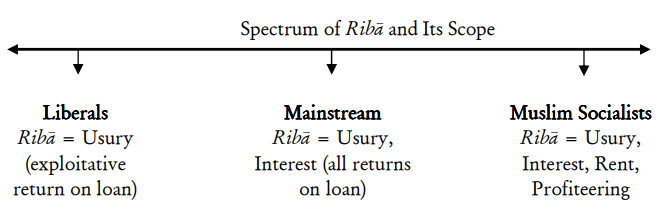
\includegraphics[width=\textwidth]{CourantsIslamContemporain/ImagesCourantsIslamContemporain/Riba.png}



The above differences have left scholars divided on several important questions that demand straightforward answers. Those questions include the following ones:
\begin{itemize}
    \item 
1. Is bank interest prohibited in the light of the Qur'an and the sunnah? If yes, how?
    \item 
2. Whether the Qur'anic term riba includes all kinds of interest rates or it relates only to the excessive interest rates?
    \item 
3. Whether the scope of riba extends to the interest charged and paid on business transactions in the banking system or is restricted to the interest charged on consumption loans only?
    \item 
4. Does Islam allow loan transactions? If yes, how and in what form?
    \item 
5. Is paying interest a lesser evil as compared to charging it?
    \item 
6. Is borrower always \textit{mazlum} (a losing party) in an interest bearing loan transaction?
    \item 
7. Does Islam allow indexation of loans on the grounds of inflation?
    \item 
8. Is credit-sale with higher deferred price as compared to the spot price allowed?
    \item 
9. Does Islam approve of “time value of money,” especially when charging higher deferred price is allowed in a credit sale?
    \item 
10. Are future currency contracts permissible in Islam?
    \item 
11. How and to what extent is salam transaction permissible?
\end{itemize}


These are but a few questions.
\begin{Synthesis}
We show in this paper that whatever confusion prevails among contemporary scholars on this subject is the outcome of following an inadequate methodology for determining the meaning and scope of riba.
\end{Synthesis}
 In fact, this methodology has mystified the nature of riba, which is otherwise clear when viewed from the methodological view point of the eminent Muslim jurists of the past. The mystification is such that not only it results in confusing answers to these questions but it also begets confusing questions. Unfortunately, the confusion has built up to the extent that the Federal Shariat Court of Pakistan has been struggling to come up with a definition of riba. It is in this background that this paper attempts to explain:

(1) the contemporary Islamic economists' methodology of interpreting and classifying riba; (2) why this methodology is wrong and insufficient; (3) the methodology of understanding riba on the pattern of Muslim jurists of the past; (4) that the methodology given by the Muslim jurists is coherent and compact.

The reader will encounter a number of arguments in this paper that are advanced by those who justify bank interest. Since the paper deals with the legal substance and not with the economic merits of arguments, hence we will restrict ourselves to the legal analysis of those arguments and leave aside their economic analysis and rationale, which require an altogether different methodology. Any legal system has three aspects: (1) what: the legal rulings (i.e., ahkam); (2) how: the rules of deriving those legal rulings (i.e., usul al-fiqh); and (3) why: the underlying rationale(s) and wisdom behind the legal rulings (i.e., hikmah)

It is important not to mix these aspects. The present study deals with the first two aspects of the issue of riba. Moreover, the classification of riba discussed in this paper is primarily based on the methodology of Hanafi jurists for ensuring analytical consistency. We presume that a school of law represents an internally coherent system of interpretation and that mixing up the views of the various schools results in inconsistencies.7 However, views of the other schools have been briefly mentioned in the footnotes wherever required. Finally, the paper does not attempt to show that the Hanafi jurists' approach is superior to all others, rather it explains that the classical jurists' approach (whether Hanafi, Maliki, Shafi‘i or Hanbali) to understanding riba is superior to that of the modern scholars. The methodology of these jurists share several common results that are important in order to answer the above questions.

Following section outlines the method adopted by modern Muslim scholars and economists. The next section discusses problems in this methodology and develops the skeleton for the methodology that is then applied in the coming section, which details out the general rules of riba alongside their resulting implications. The last section concludes the paper by giving a comprehensive definition of riba based on discussions in sections three and four.


\newpage
\subsection{Outline of the Mystifying Methodology}

Imran Ahsan Khan Nyazee\sn{\href{https://en.wikipedia.org/wiki/Imran_Ahsan_Khan_Nyazee}{Pakistan} Nyazee's academic career was inspired by the work of Abdur Rahim. Nyazee argues firstly, that due to its unique set of principles of interpretation, each school of Islamic law represents a theory of law unto itself. Secondly, he points out that Istiḥsān cannot be understood without understanding of the workings of qiyās. It is, therefore, difficult to accept that there was no system of interpretation before al-Shāfi‘ī's time. Thirdly, he concludes that the uṣūl al-fiqh never existed. Furthermore, Nyazee describes beyond the individual fikh of each school of law, another theory of interpretation called maqāṣid al-sharī‘ah (theory for the purpose of the sharī‘ah) which was developed by al-Ghazālī. Nyazee has written and self-published on a number of aspects of Islamic law. He agrees with most Muslim scholars that strictly speaking, selling money (taking interest) is prohibited, according to Islamic law. Some point out a difference between the treatment of riba in the Qur'an versus the Sunnah but Nyazee the two approaches are actually one and the same.Nyazee also proposes that all loans (except those of a charitable nature without a fixed period of repayment) and therefore all banking is prohibited and unIslamic. Nyazee is equally intolerant of murabaha, the Islamic system of business where in-put costs and mark-ups are made transparent between vendor and buyer. He argues riba will inevitably enter such transactions.[10] He extends the prohibition to the creation of wealth on the basis of debt and the fractional reserve banking system. These elements along with zakat (the system of alms-giving) he says, are the differences between Islam and capitalism. He advocates the use of the gold and silver dinars and dirhams as the currency of the Muslim community. Nyazee would also prohibit the corporation or 'legal personality' under Islamic law.} explains that the methodology adopted by modern scholars for determining the meaning of riba is the same, though they disagree in their conclusion regarding whether or not bank interest is riba.8 The fundamental problem of their methodology lies in overlooking the inherent link between the Qur'an and sunnah. This methodology of interpreting riba was initiated by Muhammad Rashid Rida (d. 1935) \sn{voir p. \pageref{Theol:Rida} Frère musulman pas le voyage en Europe. Plue el manar un commentaire coranique, sensé être l'héritage d'abdu}, which goes as follows:9

\paragraph{Lecture de Rida El Manar}
Riba is classified into two categories, riba of the Qur'an (also equated with riba 'l-nasi'ah, i.e., interest on loan transaction) and riba of hadith (equated with riba 'l-fadl, i.e., interest on exchange transaction).

Rida begins with literal meaning of the word riba (excess) and then traces some riba-based transactions practiced by Arabs during the time of Prophet (peace be on him). Rida, relying on some commentators of the Qur'an, asserts that the Qur'anic verse regarding riba deals with a specific practice of Arabs known as credit-sale where the payment of price is deferred to a future period while delivery of goods takes place on spot. Because a seller is allowed to charge whatever price he wants in a sale transaction, no riba is involved in the original price negotiated between the two parties-any excess in future price becomes part of the price. However, they used to increase the price excessively whenever the debtor would be unable to settle his debt obligations at the end of payment period. The debtor was given the option, “Will you pay the debt or increase the amount in lieu of delay?”

For Rida, it was this excessive rate (doubling and multiplying) of interest in debt-based transactions added to the original sum at the end of payment period which was prohibited by the Qur'an (he called it riba 'l-jahiliyyah).10 From this, he concluded that the bank interest is not the same riba that was deemed impermissible by the Qur'an because (a) it is neither doubling and redoubling of rates (b) nor the excess is stipulated in the initial period of the banking transaction-he assumes that the initially added interest is part of the principal or original sum just like the original sum in case of credit-sale. 
\begin{Synthesis}
Hence, for Rida, only compound interest is prohibited.
\end{Synthesis} 

Other scholars, supporting Rida's view, added that business loans were not common among Arabs as theirs was a subsistence economy; loans were largely taken by poor people for consumption purposes on interest and whenever they were unable to repay them at due time, excessive interests were added to the original sum. Hence, it was this type of interest that was declared prohibited by the Qur'an and it has nothing to do with the modern commercial loans, \textbf{which are mutually beneficial for both parties.}11

Having ascribed this meaning to the Qur'anic word riba on the basis of some historical traces, Rida then explains the form of riba declared impermissible in the sunnah as a distinct prohibition from that of the Qur'an.
\begin{Def}[Riba] Usure, profit ou gain réalisé sur un prêt.
\end{Def}

\begin{Def}
[Riba al-buyu] : Usure. Opération de vente dans laquelle une matière première est échangée contre la même matière première mais en quantité différente et la livraison d’une des matières premières est postposée. Pour éviter le riba al-buyu, les matières premières échangées par les deux parties devraient être en quantités égales et l’échange devrait être instantané. Riba al-buyua a été condamné par le Prophète Muhammad afin d’éviter que le riba (intérêt) n’affecte insidieusement l’économie.
\end{Def}
\begin{Def}[Riba al-duyun] : Usure d’une dette.
\end{Def}
 
\begin{Def}[Riba al-fadl] : La différence de quantité entre deux biens échangés et comportant du riba.
\end{Def}
\begin{Def}[Riba al-nasiah] : La différence de paiement liée au report de deux biens comportant du riba
\end{Def}\mn{cf Glossaire des termes financiers  Islamiques \href{https://www.cairn.info/la-banque-et-la-finance-islamiques--9782804167042.htm}{Banque et finance islamique} } He calls it \textit{riba 'l-fadl} which emerges in the exchange of two counter values of the same or different species and hence also called \textit{riba 'l-buyu‘}.12 The position of Rida, which may be termed as minority view, is summarised in figure 2.


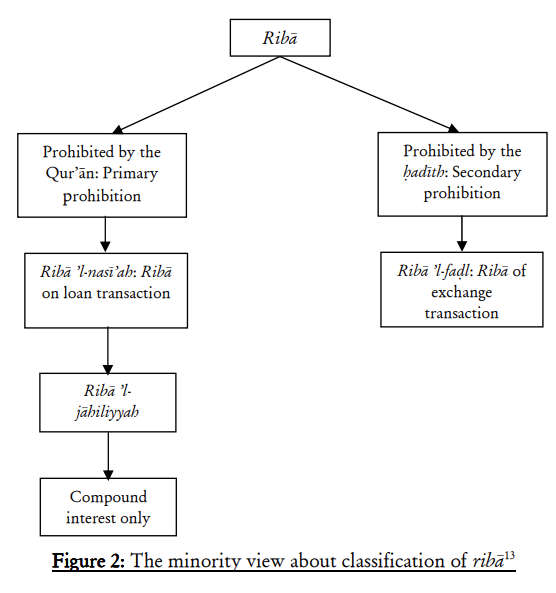
\includegraphics[width=\textwidth]{CourantsIslamContemporain/ImagesCourantsIslamContemporain/RibaRida.png}

Thus, Rida dichotomised the two concepts of riba, one attributed to the Qur'an and another to the sunnah. He finally declared the first one as real or explicit riba while latter as lighter or implicit riba.
\textbf{
Though the majority of contemporary scholars did not agree with the conclusion drawn by Rida about legitimacy of bank interest, however they adopted his methodology of classifying riba. The only difference in their opinion is that riba of the Qur'an includes all rates of return on loan and it is not merely restricted to the compound interest of jahiliyyah}\sn{la période pre islamique}


To them, business loans were a part of Arab's economy and any contractual return to lender is unfair because this is tantamount to refusing to share business risk with the borrower. We can depict their views in figure three.
\begin{Synthesis}
On a donc un nouveau problème, le pret commercial lié avec l'industrie et face à ce nouveau problème, une lecture de Rida qui est assez positive (Riba = Excess) mais qui note une différence entre Coran et Sunna) et fait une distinction entre les deux, reprises ensuite par les autres légistes, mais en repartant d'une lecture stricte du Riba comme intérêt. Il conveint d'articulier Coran et Sunna de façon non parallèle mais l'un par l'autre.
Il convient de montrer l'évolution du prêt commercial au XIX
\end{Synthesis}
Because the sunnah is not linked with the Qur'an in this methodology, both the minority and majority Muslim economists have struggled to explain as to why someone would engage in exchange transactions of the forms mentioned in hadith. Some opined that these transactions are declared impermissible because they may open the path for the “real riba” (i.e., riba of the Qur'an).


14 Others assumed that it was meant to discourage the practice of barter exchange and promote market exchange through a medium of exchange.15 Yet another view argues that it eliminates the possibility of benefiting from asymmetric information of the contracting parties.16 The truth is that none of these explanations makes the point.

2.1. The Nature of Debate within Minority and Majority Schools

The debate that has taken place within the followers of this mystifying methodology on the issue of why or why not bank interest is riba may briefly be summarised here. As explained above, Rida asserted that bank interest was not included in the Qur'anic concept of riba of debt because it was different from the riba that was charged by Arabs on credit-sale transaction by doubling and multiplying the price whenever the debtor was unable to settle his debt at due time and asked for relaxation in payment period.18 Rida explained that the Qur'anic verse “Allah has permitted bay‘ and prohibited riba”19 referred to this riba. To strengthen his case, he argued from the verse: “O Believers! Do not devour riba doubled and multiplied and fear God so that you may prosper.”20

This verse complements the former verse in the sense that what was implicit in the first verse was made explicit in the latter-both verses referred to the practice of doubling and multiplying of interest and none of them forbad the bank interest.

How do the majority of scholars respond to this argument? For example Usmani notes the Qur'anic verse:

O you believers! Fear God and give up riba that remains outstanding if you are true believers. Behold! If you do not obey this commandment, then God declares war against you from Himself and from His Prophet. But, if you repent (from riba), then you are entitled to only your principal amounts. Neither should you inflict harm to others, nor others should do harm to you.21

The argument is based on the emphasised words ‘you are entitled to only your principal amounts (ra's al-mal)'. He infers from these words that the rightful entitlement of lenders is the original sum advanced; he cannot charge any increase whether small or large (doubled and tripled). To him, the verse (3:130) forbids a severe form of riba where interest is multiplied, but it does not restrict riba to this specific form. Hence, bank interest falls within the purview of the Qur'anic verse “Allah has permitted bay‘ and prohibited riba.”22 They are also of the view that charging interest on commercial loans was also practiced by Arabs.23

Does the above analysis of mainstream scholars guarantee the prohibition of bank interest? We are afraid it does not. Their arguments rest on two assumptions:

(1) The verses (2:278-79) address the issue of loan-transaction.

(2) Ra's al-mal (principal amount) can only refer to the original principal advanced in loan.

Both of these assumptions are problematic. Following submissions can be made against them:

(a) If the meaning of the verse is to be determined with reference to historical practices, one can equally claim, just like Rida, that the verse is not about loan transaction but about credit sale. In that case, ra's al-mal is not referring to the principal amount lent; rather, it is the deferred future price of the goods sold. On which legal grounds or facts can this claim be dismissed?

(b) Further, this deferred price might include increase over and above spot price. Hence, the future price could consist of two components: spot price plus some additional profit. The sum of these two would constitute ra's al-mal (principal amount) in this transaction (i.e., principal amount in credit sale (ra's al-mal) = spot price + extra profit)

Whenever a debtor was unable to repay full amount, further multiplied increase was added to this original sum, Rida called it interest. This would increase the due amount to: total amount after increase added due to delay, which is interest in addition to ra's al-mal.

Using this structure, one can then argue that the initially added interest in a loan transaction is equivalent to initially added “extra profit,” which becomes part of ra's al-mal. Therefore, entitlement to the ra's al-mal means entitlement to the simple interest, as claimed by Rida.

(a) The only legal justification for ascertaining that the verse is about loan transaction is based on the words “ra's al-mal” (principal amount). But how can it be settled that ra's al-mal here means ra's al-mal of a loan transaction? This question is important because a number of transactions constitute a component of ra's al-mal. For example, there is ra's al-mal both in mudarabah and musharakah contracts. How to exclude these forms of ra's al-mal from the purview of the Qur'anic verse? If someone says, “This verse is about loan, so ra's al-mal refers to that of loan contract and not of mudarabah and musharakah,” he is clearly arguing in circularity. The argument goes like this:

Q: How do we know that the verse is about loan contract?

A: Because the verse talks about ra's al-mal.

Q: How do we know that ra's al-mal here refers to that of loan?

A: Because the verse is about loan contract!

A circular argument is no argument.

(b) Muslim Socialists could maintain that ra's al-mal means principal amount of all business contracts. Therefore, it is not legitimate to charge any excess over and above principal amount, no matter it is mudarabah, musharakah or ijarah.

Not only that the analysis of mainstream scholars does not necessarily imply the prohibition of bank interest, it leads to a set of unsettling arguments that have left Islamic economists bewildering about some basic issues. For example,

(1) Even if it is agreed that ra's al-mal means principal amount of a loan transaction, does it mean “nominal” amount or the “real” (inflation adjusted) amount? Again, what are the legal grounds to settle this issue? Because there are no clear-cut legal grounds available in this methodology, we see scholars are divided on this subject matter-some allow indexation of loan against inflations while others do not.

(2) What about the question of “time value of money?” This question poses challenge for Islamic economists because they, as a rule, approve the practice of charging higher price in credit-sale and murabahah.

(3) The Lawgiver has allowed salam, what are the legal grounds for not extending this permission to currency salam (future currency contracts)?

Undoubtedly, majority view has addressed these issues, but the answers do not seem to be stemming out of a coherent analytical legal system. This approach is often found mixing up legal analysis with economic analysis. This missing coherent analytical legal system is the root cause of most of the mystification that has prevailed all over. It is an unfortunate state of affairs and it is high time to demystify things.

3. Methodological Assumptions of Premodern Muslim Jurists (Fuqaha') for Understanding Riba

To understand the method used by the eminent premodern Muslim jurists for understanding riba, three methodological issues (MI) need to be clarified. They are explained by Nyazee in detail.24

1) Link between the Qur'an and Sunnah

The methodology adopted by the modern Muslim scholars and economists is misleading because it delinks the Qur'an and sunnah. It assumes that the meaning of riba is different in the Qur'an and sunnah, which is not the case. To explain the nature of error made by both the groups, it should be noted that Muslim jurists (fuqaha') classified riba in the category known as mujmal (unelaborated)25 whose meaning and scope cannot be determined without explanation (bayan) of the Lawgiver (Shari‘). The famous hadith (as given in footnote 1) that explains different usurious transactions actually does not add something to the Qur'anic word riba. Rather, it defines its meaning and scope.

Thus, while to the contemporary scholars the meaning of riba is known independent of hadith and they see hadith as adding some more cases to the Qur'anic concept of riba, the jurists say that hadith is the definition of the term riba used by the Qur'an. Thus, riba 'l-nasi'ah and riba 'l-fadl both are included in the Qur'anic concept of riba.

2) Relationship between Loan and Bay‘ (Exchange)

Loan is also classified as a form of exchange transaction (bay‘)26 by Muslim jurists. The scope of this paper does not allow detailed analysis of this assertion.27 For descriptive purposes, it can be seen that a loan of Rs X is an exchange of Rs X today with Rs X after time deferment (and with Rs X + Y if interest payment of Rs Y is included). Figure 4 depicts this nature of loan transaction by illustrating a loan transaction between Mr. A and B:

3) Skeleton of a Coherent Legal System

A coherent shari‘ah-based legal system consists of a set of general rules, called

‘azimah by the jurists, supplemented by some exemptions to these laws, called rukhsah. In the words of Nyazee, ‘Azimah (lit. determination, resolution) is applied to mean a rule that is applied initially and for itself. Such rules form the backbone of the law. As against this, there may be a rule that goes contrary to the requirements of the initial rule, but is permitted by the law. This rule is considered to be a rukhsah (exemption) from the initial rule.28

This classification of ‘azimah (the higher or first order rules) and rukhsah (the lower or second order rules) is important for several reasons.

First, it explains the order in which the rules have to be applied.

Second, it explains why sometimes two opposing cases may be allowed within a given skeleton of law.

Third, the order of rules implies that an exception cannot be extended using any method of argument, whether analytical or analogical. On the other hand, extension of first order rules is legitimate by these methods. In other words, it is not allowed to build a sub-legal system based on exemptions because otherwise it starts negating the primary provisions and objectives of the law-an exemption from the general rule must remain an exemption.

Fourth, because of the logical hierarchy in the operations of ‘azimah and rukhsah, it is clear that an exemption from a rule cannot be used to nullify or change the shari‘ah status (hukm) of any other case that is derived from the general rules. Alternatively put, an exemption (a lower order rule) cannot prevail over the higher order rules.

Fifth, because all rules and exemptions are derived from nusus (the Qur'an and sunnah), hence the only justifiable exemptions are the ones, which are given in nusus (i.e., stated by the Lawgiver Himself).

We call these nusus the “facts” of the shari‘ah-based legal system in this paper. Given these “legal facts,” the task of a jurist is to derive those general rules (‘azimah) from the facts, which render these facts internally consistent and extendible on the one hand and highlight the exemptions (rukhsah), if any, on the other.29 Finally, the general rules and exemptions generate some implications, called ahkam. This skeleton of a shari‘ah-based legal system is illustrated in Figure 5. We apply this skeleton in this paper to elaborate riba.

The relevant “legal facts” used by premodern Muslim jurists to derive general rules and exemptions are quoted at the relevant places in this article. We are now in a position to take on the issue of derivation of the general rules and the implications from those “facts.”

4. Underlying Rules behind the System of Bay‘ in Jurists' Methodology

Our intention in this paper is to reveal that the apparently large and complicated system of legal injunctions (ahkam) is reducible to a few set of rules derived from fewer legal facts. We propose that a majority of ahkam (legal injunctions or provisions) governing economic transactions (buyu‘) can be derived from three broad rules:

1. Rules of riba mentioned in the sunnah. This is not a single rule, rather a set of rules as explained below.

2. Rule about the sale of goods not possessed by a person.

3. Rule about exemption that an exemption is to be treated as exemption.

Before explaining these rules, we first explain the context of the Qur'anic verses that underlies the jurists' methodology of riba to clarify the misconception that the relevant verses of Surat al-Baqarah are about loan transaction and not exchange (bay‘).

4.1. The Context of the Verses of Surat al-Baqarah

The Qur'an states that the disbelievers said, “Verily, bay‘ (sale) is just like riba.” In response to this, it was said, “Allah has permitted bay‘ and prohibited riba.” To understand why the disbelievers said this, consider these three transactions:

(a) A gives B 100 grams of gold in exchange of 110 grams of gold to be paid after one year. This is primarily a sale contract as explained previously (i.e., exchange of 100 grams gold with 110 grams gold with time lag) and involves riba (how, this will be explained in the next section but take it for granted for the moment).

(b) A asks B for 100 grams of gold in exchange of, say, 500 kg wheat at spot. This is a legitimate regular sale contract.

(c) A demands from B 110 grams of gold in exchange of 500 kg wheat for payment of price after one year: this is credit sale contract with higher deferred price as compared to spot price and is also legitimate (this is explained in section 4.3).

The credit sale was a common practice among Arabs and, therefore, they were confused as to why the transaction (a) is impermissible and (c) is permissible while the two are quite similar in nature (i.e., both are credit sales and both involve access payment). In (a), 10 grams of additional gold are paid as counter-value for 100 grams of gold for a delay of one year and similarly 10 grams of gold are paid for a delay of one year in transaction (c). It is for this reason that disbelievers said, “Verily sale is just like riba!” That is, transaction (c) (i.e., the credit sale) is similar to the transaction (a). The technical reason for allowing transaction (c) and forbidding (a) is the similarity of genus which is explained by the sunnah. This is explained in the next sections in detail, but the important point to note here is that the assumption that the Qur'anic term riba is not about sale contract, rather it is about debt, is not implied by these verses.

Thus, the verse says that Allah has approved all forms of buyu‘ (exchange transactions) except those which involve riba.30 The natural question then arises: what is this thing called riba? Has the Qur'an given any definitive description of riba?

One may make one of the two assumptions here. First, the concept of riba was largely a sort of common knowledge for everyone and, hence, it required no legal description by the Qur'an. That common knowledge is traceable by an examination of historical record of Arabs which provides sufficient legal foundations for determining the meaning of riba. As far as the details of riba in the sunnah are concerned, they were additions over and above to that common knowledge of riba and most of these additions were unknown to the Arabs. The liberals and mainstream scholars share this assumption and we believe that this assumption constitutes what we called the “mystifying methodology.”

Second, some forms of riba may be or actually known to the Arabs but these do not set the legal standard against which the Qur'anic concept of riba is to be determined. As it is a legal term, its meaning has to be sought from the Lawgiver. In technical sense, the jurists call it mujmal (unelaborated) for which elaboration (bayan) is sought from the Lawgiver. This elaboration of the legal meaning of the Qur'anic term riba is given by the sunnah. After this elaboration by the Lawgiver, its meaning is determined definitively and it becomes mufassar (elaborated). This is the methodological assumption that the jurists use not only for defining riba but also for other legal terms of the Qur'an, such as salah, zakah, and so on.31 Thus, according to this second assumption, the practices and concepts of Arabs may be referred by the Qur'anic concept riba but it is not the benchmark against which we assign legal meaning to the Qur'anic terms.

For example, the Arabs had some concepts about how to offer salah (prayer), but this information does not define the legal meaning of the Qur'anic term salah nor is this concept limited to this information set. Similar is the case with riba. The Arabs might have been aware of some forms and practices of riba but that does not constitute the legal definition of riba. When the jurists classify a term as mujmal, they mean that this term is a technical legal term and its meaning should be determined with reference to the words of Lawgiver Himself, neither by the linguistics (dictionary) nor by the historically known social concepts and practices that hover around that technical term. It should be emphasised here that considering riba as mujmal does not mean that the Arabs did not know the meaning of this word at all. Nor does it mean that the pre-Islam Arabs did not identify certain transactions as riba-in fact they did and the jurists did consider it part of riba.32

It only means that the meaning of riba in Islamic law is not limited to, and is not based on its usage in the pre-Islam Arabia. The Qur'an and the sunnah added several shades of meaning to this concept. That is why, it became a “technical term” of Islamic law. Hence, its meaning and scope cannot be determined by its dictionary meaning or its practice and understanding by the pre-Islam Arabs. Rather, it must be determined by the Qur'an and the sunnah, like any other legal term such as salah and zakah. Just as we cannot classify concept salah as salah of the Qur'an and salah of hadith, similarly we cannot dichotomise riba. Once it is established that the meaning of riba must not be gathered from pre-Islamic usage and practices but from the Qur'an and the sunnah, the next question is: how to explain the various usages of riba in the Qur'an and the sunnah? The answer, as per the well-established methodology of the jurists, is to consider the sunnah as the elaboration of the mujmal verses of the Qur'an.

This methodology is employed by the jurists for determining the meaning and scope of salah and zakah as well as riba. Let's follow through the path of righteous ones here and have its blessings.

4.2. General Rules of Riba When Transacted Species are Same

Keeping these in mind, one has to understand the classification of riba in the system of Muslim jurists. Because the sunnah defines riba, note the words of hadith,

When you exchange gold for gold, silver for silver, wheat for wheat, rice for rice, dates for dates, and barely for barely, then exchange like for like (in equal measure) and exchange them hand to hand (at spot), else it will be riba.33

To understand what it says, consider these transactions:

1) exchange of 1 gram gold for 1 gram gold on spot;

2) exchange of 1 gram gold for 2 grams gold on spot;

3) exchange of 1 gram gold at spot for 1 gram gold with delay;

4) exchange of 1 gram gold at spot for 2 grams gold with delay.34

As per the hadith, the first transaction is allowed; the second one is disallowed because it involves excess in measurement/quantity (called riba 'l-fadl); the third transaction is also impermissible because the hadith says that the exchange of homogeneous goods is allowed in equal measurement provided it is on spot; therefore, this transaction involves the riba 'l-nasi'ah (i.e., riba of delaying); finally, the fourth transaction involves both types of riba. These transactions provide two guiding rules (R):

R 1.1) Goods of the same species cannot be exchanged immediately unless their measurement (in terms of weight or volume) is same.

R 1.2) Goods of the same species cannot be exchanged with time lag, even with same measurement.

4.2.1. Implications

Five important implications (I) should be noted.

I. 1) Impermissibility of Market for Loanable Funds

Application of rule 1.2 gives the important implication that loan, with or without interest, is prohibited in Islam because, as explained above, a loan is an exchange of homogeneous goods with time lag. Does it mean that loaning is not allowed in Islam under any circumstances? Of course, this implication of the general rule is at odd with a number of legal facts (nusus), which promise reward for offering loan to the needy ones. How to reconcile these apparently contradictory legal facts now? This is where the concept of rukhsah (exemption) is activated by the jurists. Though loaning is against the general rule (‘azimah) given by the Lawgiver, yet it is allowed by Him as an exemption from this prohibition if it takes the form of benevolent giving (tabarru‘ or sadaqah).35 Loan is classified as tabarru‘ if:

(a) it is out of the intention of benevolence to the other person (i.e., the lender consciously bestows upon the borrower the benefits associated with his asset);36

(b) no increase in its value is stipulated, else it would cease to be benevolent and would involve riba 'l-fadl; and

(c) no contractual time limit is stipulated, the lender can ask for his asset anytime he wants.37 Stipulating (legal) time constraint in loaning activity makes it a business transaction as per the application of general rules of shari‘ah and, hence, unlawful because in that case it is simply the exchange of homogeneous goods with time delay, which is not allowed, whether or not interest factor is included. Moreover, making the time period binding would imply that the lender is forced to do, or to continue with, an act of charity. This is against the very nature of charity.

In short, this principle implies that Islamic law does not permit the “market for loanable funds.” It sees loaning as an act of benevolence, especially in favour of one's relatives.38 Stated alternatively, loan is purely a social transaction (a means of tying and strengthening social bonds) in Islam and not a business. It was in this social transaction capacity that the institution of loan prevailed for thousands of centuries not only in Muslim societies but also in other civilisations of the world until the emergence of capitalism in the fifteenth century.39 Note that this important result (impermissibility of the market for loanable funds) does not follow directly from the classification of modern scholars of Islamic economics, as the majority view allows interest-free non-benevolent loans as a general rule and not as an exemption.

This implication answers one of the important arguments in favour of bank interest given by some economists. The argument says that interest should be allowed in shari‘ah because interest is the price of capital and without interest the market for loanable funds cannot be equilibrated. Because we are not dealing with the economic merit of arguments in this paper, we ignore its economic substance and comment on its legal merit only. It is clear from the above implication now that this argument has no shari‘ah basis because shari‘ah does not allow market for loanable funds to begin with, let alone equilibrating it from shari‘ah perspective.

Before moving on to the next implication, the important implication and exemption regarding loan transactions be noted:

I 1.1) A loan transaction is prohibited, whether or not interest factor is added to it.

I 1.2) A benevolent interest-free loan is recommended as an exemption to the general rules of riba by the Lawgiver.

I. 2) Impermissibility of Bank Interest

All forms of bank interest, whether simple or compound, are prohibited by Islam as per Rules 1.1 and 1.2. Similarly, the fact whether loan is made for business or consumption purposes makes no difference to this result. There remains no confusion about these conclusions if the shari‘ah rules are applied with consistency. In fact, the practice of charging interest by the bank includes both kinds of riba and it, therefore, may be stated that it is the most comprehensive form of riba! This can be verified from the figure 6, which depicts detailed structure of riba-based transactions in case of homogenous goods (leaves aside heterogeneous goods for the moment).

I. 3) False Dichotomy between “Giving and Taking” Riba

The recipient of riba is not always the lending party as is usually perceived. It can be seen from above examples that in case of transaction (2) the lender is the beneficiary of riba, but in transaction (3) riba is received by the borrower, and finally both are its recipients in transaction (4). Hence, opinions such as “taking riba is a greater evil than giving it and, hence, paying interest to the bank is a lesser evil” are based on the fallacious assumption that it is only the bank that receives interest in a typical interest-bearing loan transaction. This wrong assumption is the outcome of using the wrong methodology outlined in section two.40

I. 4) Mutually Beneficial Riba is Prohibited

The view that bank interest realised in transaction (4) is or should be permitted (as claimed by liberal Muslim scholars) is implicitly based on the assumption that “two wrongs make one right”-that is, it assumes that mutually enjoyed riba of the lender and borrower can make this transaction acceptable while the matter of fact is that each of them is separately prohibited to begin with.

I. 5) Irrelevance of Time Value of Money

Following the wrong methodology has resulted in another confusing argument that the bank interest should be allowed because of “time value of money.” This argument is based on the presumption that Rs. 1 today is worthier than Rs. 1 tomorrow. Why? Economists believe that this is due to the subjective time preferences of an individual. A rational (i.e., self-interested utility maximising) economic agent is said to have positive time preferences in the sense that consumption today is preferred to consumption tomorrow because the latter is uncertain, which makes him impatient, thus he wants to have it today than tomorrow.

Another reason for having this positive time preference emerges from the institutional arrangements: if I have the option of earning some interest (say Rs. Y) on Rs. 1 by putting it in a bank account today, why should I lend it to someone for free? Putting Rs. 1 in a bank account will make it “Rs. 1 + Rs. Y” for sure (assuming away bank insolvency), say, after one year while lending it to someone will leave it worth Rs. 1. Hence, Rs. Y (which may be expressed in percentage) is the price that should be paid to the lender for a loan of one year, else it would be unfair with him. This argument is more of economic than legal in its substance, however, some comments can be made here to evaluate its legal substance in the light of preceding discussion.

The relevant part of the proposed argument is the second one (the institutional arrangement) because the first one is merely a subjective feeling, which may differ from person to person (as a matter of fact, not everyone prefers to consume more today than tomorrow). The argument presumes that there exists and should exist a well-established legally functional market for loan, which coordinates interest-based loan transactions. But just recall “I.1” that Islam does not approve of the market for loan to begin with. Eliminate this institution of market for loan, and the argument disappears. The point is that the concept of “time value of money” conceived in this economic sense is alien to the discussion of riba. Its validity presumes that there exists a legal institutional market for loanable funds where money is growing continually and, therefore, an individual always has the option of putting his money in that market.

Not only that this assumption is invalid from the point of general rules of shari‘ah as explained, it is also in contradiction with the ontological structure of the universe and economic facts.

The above is not the only format of this argument, it is phrased in some other shades as well. For example, it is stated that money could buy benefits and had the lender not lent it he could have benefitted himself. This implies that lending is an act of sacrificing the benefits associated with money. Therefore, the lender should be compensated for this sacrifice and interest payment is exactly that reward. This reward makes sense given that the borrower takes benefit out of money. The argument is valid to the point that money is beneficial to the lender and that if he makes the choice of not lending it, he can benefit from it. Moreover, it is also true that the borrower enjoys the benefits associated with the money. None of these facts is denied by the shari‘ah rules. But these facts alone cannot formulate the required case for this argument; it requires a moral statement in its premise to derive the desired conclusion.

To see this, note that the argument does not end here, after quoting these facts it then makes a moral assertion: “it is morally (and hence legally) right if money is lent for reciprocal benefits.” Addition of this moral statement is necessary for validating the conclusion that “interest is the just reward for lending.” But this moral assumption contradicts the general rules of the shari‘ah, which are laid down above. Seeking reciprocity in loan is exactly what that changes its status from tabarru‘ to loan as a business transaction and, hence, it becomes nothing but riba. The argument here is quite straightforward:

The owner of money is granted the right of benefitting from his money by shari‘ah rules; he is given the option of making a conscious choice of transferring the benefits associated with his money to another person as an exception to the general rules by the shari‘ah, but there is neither any general rule nor any exemption from the Lawgiver that assigns him the right of lending money in the name of the so-called “mutual benefits” (refer to I. 4 above). Legally speaking, this involves both riba 'l-fadl (because the homogeneous goods are exchanged at different rates) and riba 'l-nasi'ah (because time stipulation is invoked-the lender asks for the excess of measurement for parting with the benefits of his money for a specified time).

Another variant of this argument comes with the heading of “effects of inflation on money.” We deal with it in the next section.

4.3. General Rules of Riba when Transacted Species are Different

What about the exchange of heterogeneous goods? The last words of the hadith are as follows: “If these species differ, then exchange as you like as long as it is from hands to hand.”

They give an immediate rule:

R 1.3) Goods of the different species can be exchanged with difference in measurement.

This rule says that such goods can be exchanged at different rates as far as measurement is concerned. In other words, riba 'l-fadl does not apply in case of heterogeneous goods. Is riba 'l-nasi'ah (prohibition of time delay in payment) also not applicable in this case? Apparently, it seems that it is not because of the words of hadith, “exchange should be on spot.” This has an odd implication that credit sale (sale of goods against money where payment is deferred to future time period) is not permissible under the shari‘ah rules. This is so because credit-sale is an exchange of heterogeneous goods with time lag. But the legal facts reveal that the Lawgiver has allowed credit-sale.41 How to explain this? Is credit sale also an exemption to the general rule, like a loan transaction? The answer is: “No, it falls within the general rules.”

To see how credit-sale is permissible within general rules, one needs to dig deep into the issue of the underlying cause (‘illah) that the Muslim jurists derived from the sunnah to understand the system of riba. The relevant question facing jurists was: Is prohibition of riba restricted only to the six goods named in the hadith or is it extendible to other goods? The answer of the jurists is, yes, it is extendible and for this extension they derived the underlying cause due to which riba was declared prohibited by the Lawgiver. Keeping aside the technical details and arguments, it should be noted that some of the goods are measured in terms of weight while others are measured in terms of volume. In the hadith under discussion, gold and silver were weighable while the other four items were volumeable at the time of Prophet (peace be on him).42 Based on this classification, the jurists derived two further rules:

R 1.4) when species are different but their method of estimation is the same (such as gold vs silver or wheat vs rice), unequal quantities can be exchanged, provided that the exchange is immediate;

R 1.5) when species are different and their method of estimation is also different (such as gold vs wheat), unequal quantities can be exchanged with time delay.43

Thus, the credit sale is allowed due to the application of Rule 1.5. To see this, consider these combinations of transactions:

1) Exchange of 1 gram gold at spot for 2 gram silver on spot (method of estimation same)

2) Exchange of 1 gram gold at spot for 2 gram silver in future (method of estimation same)

3) Exchange of 2 kg wheat at spot for 1 gram gold/silver on spot (method of estimation different)

4) Exchange of 2 kg wheat at spot for 1 gram gold/silver in future (method of estimation different)

The first transaction is allowed but the second is not because when species are measured by same method (i.e., “weight” in this case), then difference in the measurement (fadl) is allowed but deferment (nasi'ah) is not permissible. The third and the fourth transactions are allowed because here not only the transacted species are different but also their method of measurement (one was measured in “weight” while the other in “volume”).

In short, when both of the similarity factors (i.e., species and method of measurement) are found, then both fadl (excess of measurement) as well as nasi'ah (excess of time delay or time deferment) are prohibited. When similarity of measurement is found alone, then fadl is allowed but nasi'ah is prohibited. Finally, when none is found, both fadl and nasi'ah are allowed. Figure 7 depicts all of these rules completely (discussion about the last layer of boxes on the right-hand side of this figure is coming next).

The preceding discussion shows that the hadith explaining the nature of riba was not about the actual practices of Arabs that begged some economic explanations with which Muslim scholars have been struggling. Rather, it stipulated the rules of exchange. It says, “If at all you make exchange transactions, here are the governing rules.” Thus, all transactions that correspond to these general rules are allowed while those in contradiction with them are prohibited (however, some are exempted by the Lawgiver).

4.3.1. Implications

Following implications are derived from the above rules. It is important to note that the first two transactions mentioned in sub-section 4.2 belong to the case when method of estimation of the heterogeneous goods is same while the latter two cover the cases when their method of estimation is different.

I. 6) Placement of Regular and Credit-Sale

Transaction (3) is categorised as regular sale transaction (usually termed bay‘) by the jurists. On the other hand, transaction (4) covers credit sale, which may take two forms: with or without extra profit margin as compared to the spot sale. Because both measurement as well as payment time differential are allowed in this case, hence credit sale of both forms is allowed.

I. 7) Placement of Currency Exchange

The remaining two boxes are relating to the exchange of currencies (termed as bay‘ al-sarf by the jurists). A detailed description of these requires an appreciation of some more technical classifications44 made by the Muslim jurists. However, they are beyond the scope of this paper. Suffice to say that the jurists divided all tradeable species into two: (a) currency items, which are used as means of exchange; they included gold and silver (though other goods may also be treated as currency in this system) and (b) non-currency items, (goods that are exchanged, and are not medium of exchange). They roughly included all but gold and silver.45 Given this division, the jurists broadly mention four types of transactions (buyu‘):

(1) Non-currency item in exchange of non-currency item-called barter exchange.

(2) Spot or delayed currency (say gold) in exchange of spot non-currency (say wheat) item.

(a) If both of them (gold and wheat) are exchanged on spot, it is called regular sale of goods, and

(b) if the currency price (gold) is delayed, this is called credit sale.

(3) Delayed non-currency item (say rice) in exchange of spot currency item (say gold). Here, the price of the good is paid on spot while its delivery is delayed. This is called bay‘ al-salam (advance payment) by the jurists.

(4) One currency (gold) in exchange of another currency (silver)-known as bay‘ al-sarf.

Rules regarding the first two have been discussed above. Here, we have to make some submissions regarding this fourth type of transaction. Because this transaction comes under the umbrella of “different species with same method of measurement,” it is clear from figure 7 that the excess of measurement is allowed in this transaction while time deferment is not. This gives two further rules under rule (1.4):

1.4a) If different currency items (such as gold and silver) are exchanged, then it is allowed to exchange them at any rate;

1.4b) if different currency items (such as gold and silver) are exchanged, then it is not allowed to exchange them with time deferment.

If it is accepted that modern currencies are just substitutes of gold and silver, then two further important results emerge from this discussion:

I 7.1) Future Currency Contracts are Prohibited

Rules (1.4a) and (1.4b) imply that the spot currency transactions are allowed while their future contracts (known as currency salam in Islamic finance literature) are prohibited in Islam as they come under the purview of riba 'l-nasi'ah.

I 7.2) Indexing of Loans is Prohibited

Indexing the value of the currency loans against some underlying assets (say gold) on the ground of inflationary pressures is not allowed. It is often argued that since the value of currency decreases over time due to the presence of inflation, hence an extra-payment equal to the rate of inflation, over and above the original sum given in loan, should be allowed in favour of the lender to keep his purchasing power. Again, because the economic merit of this argument is beyond the scope of discussion in this paper, we restrict only to its legal merit. If it is accepted that one rupee is legally nothing but equivalent of 1 unit of gold or silver (whatever that unit be), then Rules 1.1 and 1.2 (governing the loaning contract in gold or silver currencies) should automatically become operational.

Those rules imply that (a) loaning in the form of currency item is allowed if and only if equal measurement (whatever the unit of measurement) is returned; else it would be riba 'l-fadl; and (b) it is a loan made out of benevolence and not business intention (having time stipulation); else it would be riba 'l-nasi'ah. Hence, adding an extra amount to loan transaction in the name of “indexation” is but both, riba 'l-fadl (because of the excess of measurement) and riba 'l-nasi'ah (because the increase is time bound). 46 Again, let simplicity and sanity prevail.

I. 8) Placement of Salam

To see how the jurists accommodated salam in this scheme, note that there is nothing in the set of rules 1 (from 1.1. to 1.5) which forbids it. However, according to rule 2 (given at the start of this section), selling what one does not possess is not permissible and this is exactly what a salam transaction involves. Thus, a salam transaction should not be allowed as per the general rules of shari‘ah. We are once again faced with the same issue: salam is permitted in the “legal facts;” how and where to place it in the legal skeleton of the shari‘ah? Is there another general rule, which governs its permission as we saw in case of credit sale or is it an exemption from the general rule just like loan? The jurists' answer is the following: Salam is permitted as rukhsah-exemption from the general rules-by the Lawgiver.47

Because it is an exception, as per rule 3, it would be allowed only as “one of its kind” (sui generis) and cannot be used as justificatory mode for deriving more comparable transaction forms (e.g., currency salam). An exception to the general rule remains exception and does not turn into a rule for other cases because then it ceases to be an exception and creates a situation of self-contradictory general rules, which is not acceptable in any legal system. Thus, salam transaction is allowed as an exception for those transactions where (a) a currency item is exchanged against a non-currency item and (b) non-currency item is deferred while the currency-item has been paid at spot.48 This is what the exception is all about; one cannot extend this exception to the transaction types where currency items are exchanged with each other because that would violate condition (a) of the exception case.49

Figure 8 shows a map of interplay among legal facts (nusus), general rules, exemptions, and the derived implications related to riba and bay‘ that are discussed in this paper. This diagram shows that a rather complex looking system of ahkam (implications) showing up at the ending layer boxes of figure 8 emerge out of a set of general rules, which are derived to make underlying legal facts compatible with each other.

5. Conclusion: The Definition of Riba

We conclude this paper by elaborating a comprehensive definition of riba that can be inferred from the discussions in this paper. Let's quote it from al-Sarakhsi:50
\begin{Synthesis}
Riba in its literal meaning is excess... and in the technical sense (in the shari‘ah), riba is the stipulated excess without a counter-value in bay‘ (sale).51
\end{Synthesis}


Let's explain it noting several points about this definition:

(1) Muslim jurists do not introduce the word loan in the definition of riba because they categorise loan transaction under exchange (bay‘). Not appreciating this point resulted in the misconception that since the fiqh conception of riba does not deal with the subject of bank loans, it needs to be inferred directly from the Qur'an.

(2) Riba is excess, either in the form of quantity (qadr) or in the form of benefits of delay (nasa'). The first is called riba 'l-fadl while the latter is called riba 'l-nasi'ah.

(3) This excess is without any counter-value permitted by the shari‘ah. Thus, the excess of quantity paid in lieu of time delay in case of interest-bearing loan is not allowed because these two cannot be the legitimate counter-values (see I. 4).52 For a substance to be counted as counter-value, it must be recognised by the general rules of the shari‘ah to begin with.53

(4) The excess is stipulated in exchange. If the excess is granted voluntarily, it would not be riba.

We started off with specific questions in the introduction. The appendix lists down the answers to these questions in the light of the above definition of riba. It can be seen that once the discussion about riba is placed on the right track, right and clear cut answers start emerging automatically.

Appendix: Questions and their Answers that Follow from the above Analysis

Notes

1 For detailed arguments of this position, see Abu 'l-A‘la Maududi, Sud (Lahore: Islamic Publications, 2000), 110-12; M. Umer Chapra, “The Nature of Riba in Islam,” Hamdard Islamicus 7, no. 1 (1984): 3-24; Muhammad Shafi‘, Mas'alah-i Sud (Karachi: Idarat al-Ma‘arif, 1996), 43-47; Muhammad Ayub, “What is Riba? A Rejoinder” Journal of Islamic Banking and Finance 13, no. 1 (1996): 7-24; Muhammad Taqi Usmani, The Historic Judgment on Interest Delivered in the Supreme Court of Pakistan (Karachi: Idarat al-Ma‘arif, 1999), 12-16; Mohammad Nejatullah Siddiqi, Riba, Bank Interest and the Rationale of Its Prohibition (Jeddah: Islamic Research and Training Institute, 2004), 45-48; and Mahmoud A. El-Gamal, Islamic Finance: Law, Economics, and Practice (Cambridge: Cambridge University Press, 2006), 46-52. Within this category, there are further two approaches.

One approach that represents traditional ‘ulama' emphasises the resurgence of only those business contracts that were approved by the early Muslim jurists. It proposes profit-and-loss sharing (PLS) as an ideal alternative to riba. Though it does not deny the permissibility of other than PLS-based financing instruments such as murabahah and ijarah, yet it affirms that equity-based financing method is the primary means of achieving desirable economic objectives. The second approach is pragmatic one. It justifies a more liberal and flexible stance on structuring shari‘ah-compatible transaction forms that looks for financial engineering to meet all demands of modern banking customer.

2 Muhammad Rashid Rida (d. 1935) was among the foremost proponents of this theory. See his al-Riba wa 'l-Mu‘amalat fi 'l-Islam (Cairo: Dar al-Manar, 2007). Also see Sayyid Yaqub Shah, “Islam and Productive Credit,” The Islamic Review 47, no. 3 (1959): 34-37; Fazlur Rahman, “Riba and Interest,” Islamic Studies 3, no. 1 (1964): 1-43; Timur Kuran, “On the Notion of Economic Justice in Contemporary Islamic Thought,” International Journal of Middle East Studies 21, no. 2 (1989): 171-91; Izzud-Din Pal, “Pakistan and the Question of Riba,” Middle Eastern Studies 30, no. 1 (1994): 64-78; and ‘Abd al-Karim Athari, Sud Kiya Hay? (Mandi Baha' al-Din: Anjuman-i Isha‘at-i Islam, 2008), 8-12 3 Constant J. Mews and Ibrahim Abraham, “Usury and Just Compensation: Religious and Financial Ethics in Historical Perspective,” Journal of Business Ethics 72, no. 1 (2007): 1-15.

4 See Ghulam Ahmad Parvaiz, Nizam-i Rububiyyat (Lahore: Idara-i Tulu‘-i Islam, 1978).

5 Rafi‘ Allah Shihab, Kirayah-i Makanat ki Shar‘i Haithiyyat (Lahore: Kitab Ghar, 1981).

6 Ziaul Haque, “The Nature and Significance of the Midieval and Modern Interpretations of Riba,” The Pakistan Development Review 32, no. 4 (1993): 933-46.

7 For details, see Imran Ahsan Khan Nyazee, Theories of Islamic Law: The Methodology of Ijtihad (Islamabad: Islamic Research Institute, 1994), 9-12.

8 Nyazee, The Concept of Riba and Islamic Banking (Islamabad: Institute of Advanced Legal Studies, 1995), 11-19. Imran Ahsan Khan Nyazee (b. 1945) is a well-known scholar and a prolific writer on the subject of Islamic law and is a former Professor of law in International Islamic University, Islamabad. His major works include Theories of Islamic Law; Islamic Jurisprudence; Islamic Law of Business Organization; and The Concept of Riba and Islamic Banking. He also translated some of the classical texts on Islamic law and jurisprudence, including: Hidayah of Marghinani; Bidayat al-Mujtahid of Ibn Rushd; Amwal of Abu ‘Ubayd; and first two volumes of Muwafaqat of Shatibi.

9 Rida, al-Riba wa 'l-Mu‘amalat fi 'l-Islam, 69ff.

10 Period before the advent of the Prophet (peace be on him) is referred to as jahiliyyah (i.e., the period of uncivilised state of affairs).

11 Fazlur Rahman, “Riba and Interest,” 7-8.

12 In this regard, a hadith reads, “The Prophet said, ‘While exchanging gold for gold, silver for silver, wheat for wheat, barley for barley, dates for dates, and salt for salt, exchange like for like, in equal measure, and exchange from hand to hand. If these species differ, then sell as you like as long as it is from hand to hand.'” Muslim b. al-Hajjaj, Sahih, Kitab al-musaqah, Bab al-sarf wa bay‘ al-dhahab bi 'l-wariq naqdan.

13 Adopted from Nyazee, Concept of Riba.

14 Maududi, Sud, 118-19.

15 Chapra, “Nature of Riba in Islam,” 3.

16 Siddiqi, Riba, Bank Interest and the Rationale of Its Prohibition, 49-50.

17 Adopted from Nyazee, Concept of Riba.

18 Rida, al-Riba wa 'l-Mu‘amalat fi 'l-Islam, 69-70.

19 Qur'an 2:275.

20 Ibid., 3:130.

21 Ibid., 2:278-79.

22 Ibid., 2:275.

23 For details, see Shafi‘, Mas'alah-i Sud, 106-120 and Siddiqi, Riba, Bank Interest and the Rationale of Its Prohibition, 38-40.

24 Nyazee, Concept of Riba, 35-36.

25 Mujmal is a term used by Muslim jurists to refer to a Qur'anic term that begs its explanation through the words of Lawgiver (i.e., God and His Prophet [peace be on him]). One cannot interpret mujmal either by looking its meaning in the dictionary nor can its meaning be determined through historical practices at the time of revelation of the Qur'an. Mujmal can be elaborated only by the Lawgiver. Another example of mujmal is the Qur'anic term salah (prayer) which cannot be interpreted literally.

26 Bay‘ means exchange of counter values, and is not restricted to sale of goods/services. Abu Bakr b. Mas‘ud al-Kasani (d. 587/1191), the illustrious Hanafi jurist, defines bay‘ as “exchange of property with property” and then elaborates that the concept includes not only ordinary sale but also barter, exchange of currencies, advance payment and many other forms of exchange. Bada'i‘ al-Sana'i‘ fi Tartib al-Shara'i‘, ed. ‘Ali al-Mu‘awwad and ‘Adil ‘Abd al-Mawjud (Beirut: Dar al-Kutub al-‘Ilmiyyah, 1997), 6:532-33. Abu 'l-Hasan ‘Ali b. Abi Bakr al-Marghinani (d. 593/1197), author of the authoritative Hanafi manual al-Hidayah, also explicitly asserts that qard (loan) begins as an act of charity but becomes an exchange transaction in the end. al-Hidayah fi Sharh Bidayat al-Mubtadi (Beirut: Dar Ihya' al-Turath al-‘Arabi, n.d.), 3:60

27 See Nyazee, Concept of Riba, 45-46.

28 Ibid., 49.

29 The Hanafis use the methodology of istihsan (juristic preference) for ensuring harmony and analytical consistency within the law when general rules and legal facts seem to contradict. If something appears prohibited in the light of the general principles of law, but has been explicitly permitted by one of the texts (i.e., legal facts), the Hanafi jurists take the position that it is permissible as an exception to the general principle. They use the rule, “prohibited under qiyas but permissible under istihsan” for this purpose. Exceptions to the general principles are made on the basis of the text, consensus, necessity or some other “covered principle” (qiyas khafi), which needs to be uncovered. Muhammad b. Abi Sahl al-Sarakhsi is worth quoting here: “This [istihsan] is the evidence coming in conflict with that apparent principle (qiyas zahiri), which comes into view without one's having looked deep into the matter.

Upon a closer inspection of the rule and the resembling principles, it becomes clear that the evidence that is conflicting with this apparent principle is stronger and it is obligatory to follow it. The one who chooses the stronger of the two evidences cannot be said to be following his own personal caprices.” Muhammad b. Abi Sahl al-Sarakhsi, Tamhid al-Fusul fi 'l-Usul, ed. Abu 'l-Wafa' al-Afghani (Beirut: Dar al-Kutub al-‘Ilmiyyah, 1993), 2:200-202. Another important point made by al-Sarakhsi is that when the jurist uses istihsan and prefers the stronger rule, he abandons the weaker one and as such it is not permissible for him or his followers to follow the latter. He goes on explaining that when istihsan is carried out on the basis of a concealed or covered principle (qiyas khafi), the established rule does not amount to be an exception but becomes a general principle in itself.

Interestingly, not only the Hanafi jurists but also the Maliki jurists explicitly employ the principle of istihsan for resolving the apparent anomaly found in the legal facts where one set of nusus prohibits a loan transaction and another set of nusus allows it. They hold that it is prohibited as an exchange transaction but allowed as an act of charity.

30 Al-Sarakhsi interprets this verse as the following: “Trade is of two kinds: permitted (halal), which is called bay‘ in the law; and prohibited (haram), which is called riba. Both are types of trade. Allah informs us, through the denial of the disbelievers, about the rational difference between sale (bay‘) and riba, and says, ‘That is because they said, “Sale is like riba.”' He, then, distinguishes between prohibition and permission by saying, ‘And Allah has permitted sale and prohibited riba.' Through this, we came to know that each one of these is trade, but only one form is permitted.” Al-Sarakhsi, al-Mabsut, ed. Hasan Isma‘il al-Shafi‘i (Beirut: Dar al-Kutub al-‘Ilmiyyah, 1997), 12:1-2.

31 The famous Hanafi jurist Abu Bakr al-Jassas al-Razi (d. 370/980) says, “In the law (shari‘ah), it (riba) is applied to meanings in which it was not used in the language. This is indicated by the fact that the Prophet (peace be on him) termed nasa' as riba in the tradition of Usamah b. Zayd (God be pleased with him). He said, ‘Verily, riba is in nasi'ah.' ‘Umar b. al-Khattab, (God be pleased with him) said that riba had different forms and out of these salam in teeth, that is, in animals, is not concealed. ‘Umar also said that the verse of riba was one of the last to be revealed, and the Prophet (peace be on him) was taken away before he could elaborate the details for us. Therefore, give up riba and the suspicion of riba. It is established from this that riba became a technical term, for had it been governed by its original meaning in the language, it would not have been obscure for ‘Umar, who was fully aware of the names used in the language, being a native speaker.

This (the conversion of the word into a technical meaning) is also indicated by the fact that the Arabs were not aware of the sale of gold for gold and silver for silver with a delay (nasa') as riba, but this is riba in the technical meaning. If this (meaning of riba) is as we have explained it, then, it became like all the other unelaborated (mujmal) words that are in need of an elaboration (bayan). These are terms that have been transferred from the language to the law and assigned meanings to which the word was not originally applied in the language, like salah, sawm, and zakah. Such words are in need of a bayan and it is not proper to employ them in legal reasoning for the prohibition of any of the contracts, unless an evidence has been adduced to show that such a meaning is employed by the law.

The Prophet (peace be on him) elaborated on many occasions the intention of Allah in a verse, by way of an explicit statement or in response to a query (tawqif), and through these he has indicated the evidence (dalil). The (legal) meanings are, therefore, not lost to those who have knowledge when they employ legal reasoning.... In the technical sense, the word riba is assigned several meanings. The first is the one that was prevalent among the people of the jahiliyyah. The second is excess in the same species out of things measured and weighed, according to the view expressed by our (Hanafi) jurists.... The third is nasa' (delay), which is of several types.” Ahmad b. ‘Ali al-Razi al-Jassas, ed. Muhammad al-Sadiq al-Qamhawi, Ahkam al Qur'an (Beirut: Dar Ihya' al-Turath al-‘Arabi, 1992), 2:183-84. Al-Sarakhsi is also worth quoting here:

“Mujmal is the word the meaning of which is not understandable except by asking the one who used this word.... An example of mujmal is the saying of the Almighty: “He prohibited riba” as riba literally means excess but we know that this is not meant here because sale has been permitted for the purpose of excess. Rather, riba here means prohibition of a sale due to an excess without a counter-value stipulated in the contract; and this excess is either in the form of increase in measure or by way of delay.... It is obvious that this elaboration is not known by literal analysis. Rather, it needs a separate source. Hence, it is mujmal with respect to its intended meaning. The same is the case of salah and zakah. They are also mujmal because their original literal meaning is prayer and growth, but because of their use in specific legal acts, their intended meaning cannot be gathered from their literal analysis.” al-Sarakhsi, Tamhid al-Fusul fi 'l-Usul, 1:168-69.

32 See al-Jassas, Ahkam al-Qur'an, 2:183-84.

33 Muslim, Sahih, Kitab al-buyu‘, Bab bay‘ al-ta‘am bi Mithlih.

34 One can simply substitute “Rs.” for “gram gold” in these transactions if Rs. (currency) is treated as substitute of gold and silver currency.

35 The famous Hanafi manual Hidayah explains the position of a loan transaction in the following words: “It is an act of charity in the beginning and that is why it is not valid from a person who does not have the capacity to do charity, such as a minor or a guardian (of a minor). However, at the end, it becomes a contract of exchange because it turns into exchange of dirhams with dirhams with delay, and that is riba.” See al-Marghinani, 3:60. The commentators explain, “This necessitates invalidity of loan but the shari‘ah has recommended it and the whole ummah agrees on its validity; hence, we hold that it is valid but not binding (and can be terminated at will by any party).” Akmal al-Din Muhammad b. Mahmud al-Babarti, al-‘Inayah sharh ‘ala al-hidayah (Bulaq: al-Matba‘ah al-Kubra al-Amiriyyah, 1316 AH), 5:273. The same position is upheld by Maliki jurists.

Thus, the famous Andalusian Maliki jurist Abu Ishaq al-Shatibi (d. 790/1388) says, “There are many examples of istihsan in the law, such as loan, which is riba in reality because it is exchange of dirham with dirham with delay; but it has been permitted because it benefits and facilitates the needy.” Ibrahim b. Musa al-Shatibi, al-Muwafaqat fi Usul al-Shari‘ah, ed. Abu ‘Ubaydah Mashhur b. Hasan (al-Khobar: Dar Ibn ‘Affan, 1997), 5:194-95.

36 Jurists apply the rules of ‘ariyah (commodate-loan) on these transactions because it is the nearest match for qard and the only way to legally justify a qard transaction. Al-Kasani, 10:600.

37 In much the same way as time period cannot be stipulated in a contract of ‘ariyah because no one can be compelled to do or continue with an act of charity (tabarru‘). Al-Marghinani, al-Hidayah, 3:60. In other words, making the condition of time-period binding changes the nature of the transaction and it no longer remains tabarru‘.

38 This has some income distributional as well as social consequences.

39 For an analysis of the idea of “debt as a social construct” and the transformation of this social construct to the impersonal market form, see David Graeber, Debt: The First 5,000 Years (New York, NY: Melville House Publishing, 2011, 308-60.

40 This false dichotomy is also not consistent with a number of “legal facts” (nusus). For example, in a hadith the Prophet (peace be on him), after explaining the rule of exchange among six goods, said, “Whosoever paid more or demanded more, indulged in riba.” Muslim, Sahih, Kitab al-musaqa, Bab al-sarf wa bay‘ al-dhahab bi 'l-wariq naqdan. Both are treated equally because both are the participants of “market for loan” which is not allowed.

41 The validity of credit-sale is inferred from many facts. These include the general permissibility of sale transactions such as the words of the Exalted, “Allah has permitted sale” (2:275). The jurists hold that all sales are permitted except those which have been prohibited specifically, such as sales involving uncertainty (gharar) or which stand prohibited by the operation of other principles of law, such as the prohibition of riba. The analysis in text explains that credit sale does not fall under the prohibition of riba.

42 This is the Hanafi position. The other schools classify these six items in different ways, but interestingly all classify them into two categories. The below table summarises their positions:

School Position on Gold and Silver Position on other Four Items Hanafi weighable (mawzunat) volumeable (makilt) Hanbali weighable (mawzunat) volumeable (makilt) and countable (ma'dudt) Shfi'i currency (thaman) edibles (mat'umat) Maliki currency (thaman) storable edible items (mat'umat)

The net result is that all the four schools agree on the applicability of the rules of riba on gold and silver (though for different reasons) and they come up with the impermissibility of loan transaction. For the Hanafis, they are also applicable on all items that are either weighed or volumeable (whether they are food items or not, does not matter); the Hanbalis agree with the Hanafis but add a third category of the counted items; for the Shafi‘is, the rules of riba are applicable on food items (whether they are weighed, measured or counted does not matter); the Malikis agree with the Shafi‘is but add a proviso that these food items must be such that people generally prefer to store them. These differences have interesting implications for extending the rules of riba to cases other than the six items specifically mentioned in the traditions. For details, see Nyazee, Concept of Riba, 83-88.

43 Interestingly, although the four schools have determined different ‘illah (cause) for the operation of riba on gold and silver, yet a loan transaction even if interest-free remains prohibited for all the four schools. Thus, for the Hanafis and the Hanbalis gold and silver must be exchanged on spot because they are weighable items, the Malikis and the Shafi‘is deem it necessary because gold and silver are currency items. Resultantly, despite disagreement on the ‘illah of riba, all the four schools agree that a loan transaction is prohibited as an exchange transaction and permitted only as an act of charity.

44 These include the terms ‘ayn, dayn, and thaman. For an elaboration of the meaning of ‘ayn and dayn, see Nyazee, Concept of Riba, 54-57.

45 The jurists treat gold and silver as thaman (price/currency) in exchange with all other items. Even when they are exchanged with each other (as in the contract of sarf), both of them are treated as thaman. That is why they are called thaman mutlaq (absolute thaman). Fungible items (mithliyyat) are deemed thaman if they are exchanged with non-fungible items (qimiyyat). When a fungible item is exchanged with another fungible item, such as when wheat is exchanged with barley, the parties are at liberty to consider any one of them as thaman but they have to specify it in the contract. For details, see al-Kasani, Bada'i‘ al-Sana'i‘, 7:216-17.

46 The last two implications are based on the widely accepted assumption that modern currencies are just like gold and silver currencies and should be treated as their substitutes. See Ghulam Rasul Sa‘idi, Sharh Sahih Muslim (Lahore: Farid Book Stall, 1998), 4:350-361; and Muhammad Taqi Usmani, Islam aur Jadid Ma‘ishat-o Tijarat (Karachi: Ma‘arif-i Islami, 1999). Changing this assumption can change the implications. The alternative to this view is to accept that modern money is a promise of payment, which implies that it is an acknowledgement of debt. In that case, Islamic rules of hawalah (endorsement) transaction will be applicable. Accepting this position can allow the indexation of loans since money is now treaded as value of something which it promises and, therefore, a loan can be linked to the underlying promised asset.

However, accepting the premise that “modern money is debt” leads to the result that exchange of currencies is not allowed even on spot because of another general rule of the shari‘ah, namely, “prohibition of exchanging debt for debt” (bay‘ al-kali' bi 'l-kali'). The prohibition is reported in by many scholars of hadith. For instance, see ‘Ali b. ‘Umar al-Daraqutni, Sunan, Kitab al-buyu‘, Bab nahy ‘an bay‘ al-kali' bi 'l-kali'; Muhammad b. ‘Abd Allah al-Hakim, al-Mustadrak ‘ala 'l-Sahihayn, Kitab al-buyu‘, Bab nahy ‘an bay‘ al-kali' bi 'l-kali'. Thus, one cannot maintain both of these positions simultaneously; either he has to allow indexation of loans or he has to allow exchange of currencies. For details, see Nyazee, Concept of Riba, 96-114.

47 The jurists cite traditions of various Companions who report that the Prophet (peace be on him) prohibited them from selling what they did not possess but gave exemption for salam. Al-Kasani, Bada'i‘ al-Sana'i‘, 7:101-02.

48 Some other conditions are also applicable for the validity of this transaction but they do not relate to our subject matter here. For their details, see al-Kasani, Bada'i‘ al-Sana'i‘, 7:103ff.

49 A misconception prevails regarding the nature of riba due to a tradition, “there is no riba except in nasi'ah (deferred payment transactions).” These words of Ibn ‘Abbas constitute reason that can explain the adoption of wrong methodology by the contemporary Muslim scholars. It is inferred from this tradition that the primary form of riba deals with loan transaction, which is riba 'l-Qur'an. However, several points invalidate this inference as indicated by al-Sarakhsi. See al-Sarakhsi, al-Mabsut, 12:11-12. First, the words of the hadith are quoted from Ibn ‘Abbas who initially had this opinion but he reverted from this position later on when the hadith of riba was brought to his knowledge by Abu Sa‘id al-Khudri. Second, the ahadith of riba are quoted by several Companions of the Prophet (peace be on him) through several sources. Therefore, they cannot be ignored out rightly in favour of this isolated narration.

Third, hence, it is necessary to place these words of Ibn ‘Abbas appropriately within the legal structure of the shari‘ah. Thus, al-Sarakhsi points that the words relate to the exchange of heterogeneous goods measured similarly, because in that case there is no riba except in deferment.

50 Apçna²'

51 Al-Sarakhsi, al-Mabsut, 12:109.

52 That is why, the definition of riba in al-Durr al-Mukhtar, a later Hanafi text, is given as follows: “Riba is an excess without any counter-value recognised by shari‘ah, in favour of one of the parties in a transaction.” Muhammad Amin b. ‘Abidin, Radd al-Muhtar ‘ala 'l-Durr al-Mukhtar Sharh Tanwir al-Absar, ed. ‘Adil Ahmad ‘Abd al-Mawjud and ‘Ali Muhammad Mu‘awwad (Riyadh: Dar ‘Alam al-Kutub, 2003), 7:398-401.

53 For example, if a female sells her body in exchange of mangoes, this would not be legitimate. Nor will it be legitimate if A lends Rs 1,000 to B on the condition that B will repay Rs 1,000 plus a swine.

Appendix: Questions and their Answers that Follow from the above Analysis No Questions Answers 1 Is bank interest prohibited in the light Yes, it is prohibited, because it is of the Qur'n and the sunnah? violation of rules 1.1 and 1.2. 2 Whether the Qur'nic term rib It includes all forms of interests. includes all kinds of interest rates or it This is a necessary implication of relates only to the excessive interest rules 1.1 and 1.2. rates? 3 Whether the scope of rib extends to It extends to all kinds of loans, the interest charged and paid on commercial or consumption, as business transactions in the banking shown by the application of rules 1.1 system or it is restricted to the interest and 1.2. charged on consumption loans only? 4 Does Islam allow loan transactions? If Loan is against the general rules of yes, how and in what form? Islam. However, it is permitted by the Lawgiver as an exemption to the rule if it takes the form of tabarru'. 5 Is paying interest a lesser evil as No, it is not. The assumed compared to charging interest? dichotomy is wrong, as it has been clarified by I.3. 6 Is borrower always malm (a losing No, the borrower can also be the party) in an interest-bearing loan receiver of rib as per rules 1.1 and transaction? 1.2 (see I.3). 7 Does Islam allow indexation of loans No, it does not. The demand for on the grounds of inflation? loan indexation is invalidated by rules 1.4a and 1.4b. 8 Is credit sale with higher deferred price Yes, it is validated by the application as compared to the spot price allowed? of rules 1.4 and 1.5. 9 Does Islam approve of "time value of No, it does not. In fact, the concept money," especially when charging is alien to the subject matter of rib, higher deferred price is allowed in a provided both the concept of time credit sale? value of money and rules of rib are used appropriately. 10 Are future currency contracts No, they are not. It is violation of permissible in Islam? rule 1.4b. 11 How and to what extent is salam Rule 2 implies that salam is against transaction permissible? the general rules of the shar'ah but allowed as an exemption by the Lawgiver, hence, should remain exemption as per rule 3.
 \end{quote}
 
 
 \paragraph{Chapitre 8. Islam et assurances}
 LES CAPITAUX DE L’ISLAM  | Gilbert Beaugé
 \href{https://books.openedition.org/editionscnrs/871?lang=fr}{ Islam et assurances}
\begin{quote}
    
L’assurance est-elle légale du point de vue de la Shari’a ? Ce débat aujourd’hui encore est très vif dans les pays musulmans\sn{1 En fait, quatre éléments ont permis de classer les contrats d’assurance parmi les contrats interdits par le clergé islamique : a) l’imprécision (gharar), b) le jeu de hasard (gimar), c) l’usure (riba) et d) l’échange de choses équivalentes (bai al sain bil-dain). Le travail le plus complet à ce sujet est celui de Muhammad Baltagi, Uqud al-ta’ min wigha al-figh al islami Koweit, 1982. K. Krüger donne une bonne vue d’ensemble du droit privé des États régis par le droit égyptien. Certains problèmes comme celui du riba sont analysés de façon plus détaillée, cf. Recht van de islam, 1987.}. La fonction sociale de l’assurance est tout particulièrement perçue par la population musulmane, dans la mesure où les catégories classiques du droit musulman intègrent cette valeur. Cette fonction suppose l’utilisation du principe d’assurance et, même dans un pays aussi conservateur que l’Arabie Saoudite, on ne rencontre aucune réserve à l’encontre de l’assurance sociale\sn{2 Introduit par décret royal, pp. 98 sv., n° 746 du 5.09.1969.}. En revanche, on continue à y critiquer l’assurance privée et, de temps à autre, cette critique réapparaît dans d’autres pays islamiques.

 
2 L’assurance peut se définir comme les précautions terrestres que l’on prend à l’encontre des coups du destin et des pertes matérielles, autant d’épreuves envoyées par Allah comme le sait tout musulman pieux. De ce point de vue, l’assurance peut apparaître comme le renoncement à la croyance en une prédestination, l’abandon de l’espérance en une miséricorde ou, pour le moins, comme leur limitation. A ces problèmes de nature religieuse ou morale qui, dans des périodes difficiles, comportent également un élément politique, s’ajoute, pour le musulman, la difficulté à concevoir la notion de risque et à la démarquer de celles de jeu ou de pari, afin de pouvoir en saisir la signification fonctionnelle, en rupture avec les contrats spéculatifs qu’interdit la Shari’a\sn{3 Cf. à ce sujet Al Amin Al Darir, Al Gharar wa-athauhu fil-uqud fil figh al islami.}. La discussion sur ce thème, qui se fonde sur des textes classiques de la Shari’a remontant au Moyen Age, s’est développée à la suite de l’implantation des compagnies d’assurance européennes dans l’empire ottoman, au cours de la deuxième moitié du xixe siècle, et des tentatives d’innovation des réformateurs de l’Islam, au début de ce siècle. Une opposition de type nationaliste et pan-islamique se manifesta alors à l’encontre de ces institutions capitalistes et occidentales, qui jouera un rôle non négligeable.
 
\subparagraph{HISTORIQUE DE LA NOTION D’ASSURANCE DANS LES PAYS DU MONDE ARABE}

3 La première réflexion approfondie sur la légalité de l’assurance en pays islamique tint compte de façon singulière des exigences musulmanes. Dans son ouvrage Radd al Muhttar, Ibn Abidin, représentant de l’école officielle de droit Hanafi dans l’empire ottoman, suggère en effet le compromis suivant : il serait licite d’établir des contrats d’assurance portant sur les risques encourus à l’intérieur du royaume islamique – le Dar al Islam – à condition que ces contrats soient conclus avec une compagnie d’assurance ayant son siège hors des pays de l’Islam, dans le pays des infidèles. La prise en charge du risque devrait se faire au siège de la compagnie\sn{4 Cf. l’étude complète de C.A. Nallino, « Belle assicurazioni in diritto musulmano banafita », in Oriente moderne, vol. VII, Rome, 1947. pp. 446 sv.}.

4 On estimait ainsi satisfaire suffisamment les besoins pratiques en assurances nécessités par le trafic international des marchandises, à une époque où Constantinople, Beyrouth et Alexandrie, ports par où transitait le coton, étaient les centres essentiels du commerce britannique du Levant, alors que le commerce français était davantage orienté vers les côtes d’Afrique du Nord.
 
5 Ce n’est que relativement tard, vers 1890, bien après la fondation de banques ou la création de filiales bancaires (1850), que fut créée une compagnie d’assurance à Alexandrie5. L’initiative en fut prise par trois Libanais qui reprirent la filiale d’une petite société anglaise s’occupant d’une affaire d’assurance-vie en Égypte, pour l’étendre, à partir de Beyrouth, à l’ensemble de la Syrie. Au début du siècle, au moment même où des sociétés françaises tentaient de s’établir en Afrique du Nord6, d’autres sociétés anglaises et françaises suivirent le mouvement, en Égypte puis dans les pays du Levant, tandis que la péninsulte arabique demeurait pratiquement à l’écart jusqu’au lendemain de la Seconde Guerre mondiale.

6 Le marché était peu porteur et étroit. Il s’agissait d’opérations d’assurance-vie, d’assurance-incendie et d’assurance-transport pour quelques biens importants. Ces assurances étaient souscrites par des banques étrangères ayant un intérêt particulier à le faire : par exemple, la Banque Ottomane travailla avec Eagle Star dans le domaine du crédit et de l’assurance hypothécaire. En raison de l’inflation qui suivit la Première Guerre mondiale, les polices d’assurance-vie perdirent leur valeur et il fut difficile de remplir de nouveaux portefeuilles dans un pays ruiné par la guerre. Les compagnies d’assurance ainsi que les courtiers s’orientèrent dès lors vers l’assurance des dommages et des transports à court terme. L’activité de ces entreprises était plus importante dans les pays sous influence britannique comme l’Égypte, le Soudan, la Palestine et l’Iran, alors que l’influence française dominait en Afrique de Nord ainsi que dans les pays du nord Levant, Syrie et Liban.


7 Si l’on prend l’exemple de l’Égypte, on constate qu’un système national d’assurance se mit en place, après la Première Guerre mondiale, avec la participation de trusts européens. Son évolution fut lente car le marché était étroit7 et il était nécessaire de former un personnel local. Le Conseil de surveillance introduit en 1939 maintint dans les limites du raisonnable une évolution qui, entre temps, s’était renforcée. Les pays sous influence française connurent également ce processus, sur les détails duquel nous reviendrons. Pour la Lybie, le marché italien eut une influence déterminante sur le système de l’assurance. Il connut une évolution moins marquée, mais parallèle.

 
8 La notion d’assurance privée s’imposa timidement comme instrument de la vie économique moderne dans les pays musulmans arabes. Les réserves de nature religieuse ne disparurent que progressivement : dans le secteur bancaire tout comme dans le secteur de l’assurance, les modernistes cherchèrent d’abord à obtenir des compromis. Ils tentèrent de prouver que les institutions et les pratiques que générait la vie moderne étaient compatibles avec les règlements de la doctrine islamique, mais ne tinrent pas suffisamment compte des réalités politiques et économiques8. Curieusement, le système d’assurance sociale, alors faiblement développé, fut tenu à l’écart de cette discussion. Il était, et reste toujours appréhendé, moins comme une assurance que comme une aide de l’État. Par ailleurs, jusqu’au tout début de la motorisation, les bases manquaient pour que soit mis en place un important volume d’affaires, aussi bien dans le domaine de l’assurance des personnes que dans celui de l’assurance des dommages. Dans les décennies qui suivirent la Seconde Guerre mondiale, les défenseurs du patrimoine islamique national s’opposèrent aux partisans d’une économie occidentalisée dirigée, ou tout au moins influencée, par des pays occidentaux. Sans se situer au cœur des débats, le système d’assurance fut tout de même soumis à examen critique : l’enjeu était d’établir s’il était ou non compatible avec les prescriptions de la Shari’a.
 
9 Ces discussions se développèrent à la fin des années cinquante, stimulées par un mouvement de création de compagnies nationales d’assurance et culminèrent lors d’une semaine de discussions à Damas\sn{Une telle manifestation avait eu lieu à Paris en 1951. Un des principaux orateurs, le professeur syrien Mustapha Ahmed al Zarga, démontra la compatibilité totale de l’assurance sous toutes ses formes avec la Shari’a, tandis que le professeur égyptien Abu Zahra n’envisageait que des associations mutualistes. L’ensemble des références figure dans un rapport complet de Zahra paru à Damas en 1962 : Aqd at-ta’min wa-mauqifal-shari’a al-islamiyya minhu.} : d’éminents juristes prirent position sur la question de l’assurance et l’on s’interrogea également sur la notion de risque et la manière de le définir et de le préciser dans un contexte économique. Le droit islamique, vers lequel il s’agissait de jeter des ponts, n’offrait sur ce terrain que peu de possibilités. Il fut très difficile, entre autre, de vaincre l’opposition unanime à tous les contrats sur les risques, assimilés aux jeux et aux paris\textsuperscript{10}. L’idée moderne d’une communauté organisée pour faire face à son destin\textsuperscript{11} – dont les bateaux et caravanes pouvaient fournir un exemple – et au sein de laquelle chacun participe de manière appropriée à la réparation des dommages, ne figure pas dans le droit islamique. 

\newpage
Sous cette forme, l’idée de risque demeure étrangère et incertaine\sn{ Le terme général est gharar, l’incertitude. \begin{Def}[gharar]
Gharar al-uqud signifie contrat à risque. Ils ont un rôle dogmatique. On range aussi sous cette dénomination les contrats portant sur des prestations que l’on peut préciser, mais qui ne l’ont pas été lors de la signature.\end{Def} Cf. art. « gharar », ainsi que le commentaire de l’article 484f « äegyptisches Zivilgesetzbuch von Sanhuri » (cf. supra, note 14). voir \href{https://fr.wikipedia.org/wiki/Abd_el-Razz\%C3\%A2q_el-Sanhour\%C3\%AE}{Sanhouri et code civil Egyptien}} au musulman, qui aimerait voir codifier non seulement ses devoirs religieux, mais également ses relations vis-à-vis du monde qui l’entoure. La seule chose sensiblement comparable à une assurance personnelle est le financement d’une rente à vie, sorte de rente viagère (umra) prélevée sur les bénéfices retirés de la terre ou de tout autre bien. Toutefois, une telle institution a suscité de nombreuses réserves de la part des érudits musulmans, dans la mesure où la durée de vie du destinataire restait incertaine13.

LES TENDANCES ACTUELLES
10 Actuellement, le problème des dommages est au cœur des discussions, sans qu’il y ait toutefois de différenciation structurelle entre l’assurance des personnes et celle des dommages. L’assurance trouve sa justification première dans l’idée mutualiste d’une aide réciproque contre ce qu’il est convenu d’appeler, de nos jours, les aléas de l’existence.


11 Dans son commentaire sur le nouveau Code civil égyptien, entré en vigueur en 1956, Sanhuri14, père spirituel de cet ouvrage de lois, s’interroge une fois de plus sur la légitimité des opérations d’assurance. Il se refuse à les justifier par analogie avec des contrats comportant des éléments identiques (caution et garantie), mais il fait du contrat d’assurance un contrat autonome de type nouveau. Dans la mesure où, dans le système du droit islamique, il n’existe pas de numerus clausus et étant donné que ses éléments constitutifs sont déjà reconnus, rien ne s’oppose à ce que l’on admette ce type de contrat. Quant à l’imprécision, motif d’annulation pour un tribunal suprême de la Shari’a en Égypte, il la justifie par la nécessité économique d’une telle institution et par la légitimité statistique. Il résulte de cet examen que l’assurance n’est pas une opération de type spéculatif. Pour ce qui est de l’interdiction du riba et de la perception d’un intérêt, il soutient la thèse que le riba Nasi, c’est-à-dire le report de paiement (crédit) devrait être autorisé dans la mesure où il est nécessaire. Quant à la deuxième forme du riba – l’échange injustifié de prestations différentes –, comme par exemple l’assurance-vie lors d’un décès prématuré après paiement de quelques primes seulement, il soutient qu’il s’agit d’une opération qui pourrait être autorisée pour des raisons d’intérêt social supérieur, si cela s’avérait nécessaire.
\end{quote}
\begin{Synthesis}
Assurance : au début, légal car pas depuis Dar al Islam : peut être repris ?
Ensuite, la principale question est l'imprecision juridique, mais elle ne peut être facilement réduite, même par tontine ou autre mécanismes mutualisant (d'ailleurs caravane pas bon non plus) ?
Sanhuri : c'est nouveau donc licite. Imprécision : corrigé par actuariat ! + raison sociale supérieure. A
\end{Synthesis}

\begin{quote}
    


12 L’argument mutualiste – ta awuni ou tabaduli\sn{What does \TArabe{ تبادلي }(tabaduli) mean in Arabic?

reciprocal : 96\% of use and mutual in 4\%} – fut l’argument essentiel avancé en faveur de l’autorisation de l’assurance et, en tout premier lieu, de l’assurance-dommage. Sur ce point, on peut parler d’un accord de tous les érudits musulmans : le système traditionnel de la société d’assurance mutuelle s’offre alors pour résoudre ces problèmes. Il apporte également une solution à la question des intérêts résultant d’une accumulation de capital dans la mesure où les fruits du capital sont répartis entre les adhérents. L’interdiction de l’usure perd ainsi, sur un plan moral, de sa force explosive. Certains docteurs surmontèrent les réticences à l’égard des contrats sur les risques en faisant prévaloir que l’élément dominant dans les sociétés d’assurance mutuelle est positif, puisqu’il s’agit d’un soutien dans la détresse et le malheur. Il serait donc convenable d’accepter une part d’incertitude, élément secondaire dans un contrat d’assurance par rapport aux notions d’aide et de soutien, et qui ne nuit pas à l’efficacité du contrat. En revanche, on tend à éliminer les autres formes d’assurance parce que la mentalité de profit, associée à la structure des sociétés par actions, vise à procurer des bénéfices aux actionnaires et ne saurait être justifiée par sa fonction d’entraide15.
 
 \begin{Synthesis}
 Il est intéressant de voir le même développement des mutuelles en France dans un cadre \textit{éthique}
 \end{Synthesis}
13 Après la Seconde Guerre mondiale, les marchés nationaux reçurent une impulsion décisive du développement rapide de la motorisation, occasion pour les compagnies de recettes provenant des primes obligatoires de responsabilité civile dans l’assurance des véhicules. Dans certains pays comme ceux de la péninsule arabique, l’industrie pétrolière, en pleine expansion, avait besoin d’assurer non seulement des investissements croissants sur les lieux de production mais aussi son environnement économique et social. On s’efforça donc de mettre en place une participation appropriée aux assurances pour les transports pétroliers. Quant aux compagnies aériennes nationales, elles s’assurent pour les risques inhérents au transport aérien auprès de compagnies nationales dans la mesure où celles-ci sont aptes à répondre à leur demande16.
 
14 En raison de la faible capacité caractéristique de tous les marchés arabes, la plus grande partie des risques sont couverts par une réassurance qui, il y a encore quelques dizaines d’années, était le domaine réservé des compagnies européennes. Depuis, les marchés nationaux arabes ont tenté, avec quelque succès, de mettre en place un marché commun arabe de la réassurance. Cependant, celui-ci ne dispose que d’une capacité limitée17. Ces efforts sont soutenus efficacement par l’Association des Assurances Arabes, fondée en 1963, dont les membres sont recrutés auprès des entreprises de l’ensemble des États arabes, depuis la Mauritanie jusqu’au Golfe d’Oman. Notons pour mémoire qu’un autre groupe important a été créé quelque temps après : il s’agit de l’assurance afro-asiatique, compagnie de réassurance dont le siège est au Caire. Par des colloques internationaux, mais également par des cours de formation pour cadres, on s’efforce désormais d’atteindre un haut niveau de technicité dans le domaine de l’assurance et de promouvoir une coopération dans le travail.
 
15 Cette coopération interétatique – expression du panarabisme formulée de manière la plus expresse au sein de la Ligue Arabe – avait été précédée par des aménagements internes sur les marchés arabes qui visaient à la mise en place d’une législation relative aux contrats, assortie d’un contrôle étatique. Cela fut le cas dans les États qui connaissaient une économie libérale, mais se réduisit à quelques fonctions de surveillance dans les pays où l’assurance était un monopole d’État18.

16 Depuis qu’en 1987 a été créée en Arabie Saoudite une compagnie nationale d’assurance19, il n’existe pratiquement plus un seul pays arabe qui n’ait son propre système d’assurance, fondé essentiellement sur l’assurance-véhicule. Par contre, l’assurance-vie n’a pas suivi l’évolution : les suites d’une souscription sont toujours remises en cause par l’inflation ; de plus, l’utilisation d’une devise forte n’est pas possible dans la mesure où – dans la plupart des pays – la loi prévoit expressément que les réserves constituées par les primes seront placées dans le pays20.

\begin{Synthesis}
Nécessité fait force de loi : l'assurance Auto en Arabie Saoudite
le développement du marché est comme en France lié à l'opacité du contrat (cf assurance vie et jeu au début)
\end{Synthesis}
17 Le mouvement qui milite en faveur d’une suppression de la clause d’intérêt sur les marchés arabes, parti d’Arabie Saoudite, a également gagné le terrain des assurances. Dans les pays qui interdisent l’intérêt, comme l’Arabie Saoudite, les difficultés proviennent du traitement des dépôts des réassureurs – même dans le cas de l’assurance-dommage – dans la mesure où ceux-ci n’entrent pas dans le cadre des exceptions pour capitaux étrangers. Dans le domaine de l’assurance-vie, une solution reste envisageable par la coopération avec un fond d’investissement islamique.

\begin{Synthesis}
Voir le hanbalo-wahhabisme et son influence et la gestion de l'assurance auto dans ce cadre
\end{Synthesis}

UN EXEMPLE D’ASSURANCE ISLAMIQUE
18 Un modèle intéressant a été développé par les banques islamiques qui travaillent sans prélever d’intérêt. Leur modèle principal pour le placement de leurs capitaux est la forme bien connue de la mudaraba de participation. De par sa structure, on peut la comparer à une société en participation, à un fond de placement où le déposant a une participation aux bénéfices proportionnelle au montant de son placement et où les pertes se font au détriment de celui-ci. Si on intègre la mudaraba dans le système d’une compagnie d’assurance, on obtient la combinaison suivante :

19 Il s’agit d’une caisse de décès ou, plus exactement, d’associations d’épargnants garantissant l’épargne, même en cas de décès prématuré. Les compagnies, filiales de la banque islamique, se nomment sharikat al-takaful al-islamiyya, leur slogan publicitaire est la participation réciproque garantie (mudaraba al tadamum), c’est-à-dire l’épargne garantie entre les musulmans. Les buts de la société sont présentés comme suit :

Organisation d’un soutien et d’une solidarité réciproques au sein de la communauté islamique.

Suppression dans la communauté musulmane de l’usure (riba), qui est un fléau ainsi que l’atteste le verset du Coran 2,278. « Fidèles ayez confiance en Dieu et laissez s’éloigner de vous ce qui demeure encore du riba, si vous êtes croyants. Si vous ne le faites pas, Dieu et le Prophète vous déclareront la guerre. »

20 Toute personne âgée de 20 à 50 ans peut devenir sociétaire de la compagnie. Chaque année, celle-ci verse une prime définie, dont la plus grande partie est placée à la banque islamique. Quant aux 20 \% restants, ils sont versés librement (!) par le sociétaire à un deuxième fond destiné à soutenir les familles de ceux que le destin a frappés avant qu’ils n’achèvent leur programme d’épargne. Quand l’affiliation cesse et en cas de survie, on verse au sociétaire la quote-part sur ses parts d’investissement ainsi que sa quote-part sur les bénéfices des parts fixes et, éventuellement, sur les bénéfices de ses parts au fond de soutien de l’assurance décès. Les deux fonds opèrent donc d’après le principe de la mudaraba, sans intérêts ni participation aux bénéfices des sommes investies21. Le plus grave problème posé par cette forme de placement est la garantie d’une liquidité suffisante nécessaire pour un règlement rapide des dommages importants. Les parts de l’assuré, tout comme les bénéfices réalisés par le fonds, sont soumis au Zakat ainsi qu’à l’impôt prélevé à la source (respectivement 2.5 et 5-10 \%).

21 Les banques islamiques opèrent dans les pays arabes depuis un bon nombre d’années. Sur le volume effectif d’affaires réalisé par une société observant rigoureusement les principes de la Shari’a, on connaît très peu de choses. On sait par contre que les difficultés dans le domaine de la réassurance internationale, mais également les questions de liquidité pour remboursement de dommages importants, n’ont pas été résolues de manière satisfaisante. Une sérieuse tentative dans ce sens a été la création d’une compagnie d’assurance saoudienne caractérisée par la garantie mutualiste et gérée en conformité avec les règles de la Shari’a. Son champ d’activité se limite à un secteur ne comprenant pas l’assurance-vie, dans la mesure où cet aspect est pris en charge par les filiales des banques islamiques. Seule l’expérience montrera si cette société peut, dans le cadre de ses missions internationales, ne pas se conformer aux exceptions d’usage faites pour la circulation des capitaux internationaux.
 

22 Mentionnons en conclusion que la création des instituts financiers islamiques correspondait également à l’intention de stimuler la circulation de l’argent et des capitaux dans la masse de la population. En tant que facteur économique, l’importance de l’assurance est cependant relativement faible. Le volume global des primes est estimé à moins de 1.5 \% du volume des primes dans le monde, alors que le nombre des entreprises est évalué à 10 \% des entreprises mondiales, pourcentage d’autant plus remarquable que de nombreux États ont nationalisé l’assurance ce qui réduit d’autant le nombre d’entreprises. La majeure partie des primes provient de l’assurance-automobile et de l’assurance du commerce extérieur, auxquelles il faut ajouter l’assurance de quelques grands projets industriels. L’absence d’une véritable critique de l’assurance de la part des milieux fondamentalistes est sans doute liée à son manque d’extension. La publicité pour les produits de l’assurance est faible : la notion de prévoyance n’ayant pas été encouragée chez l’individu, la part de l’assurance-vie dans le volume global des primes est largement inférieur à la moyenne. Ce serait cependant méconnaître les faits que d’en rendre l’islam responsable : l’assurance-automobile obligatoire, introduite par la plupart des pays, a été acceptée par la population, sans réserves et sans critiques. Dans quelques pays, mais surtout dans les pays de la péninsule arabique, le montant de l’assurance est pris en considération pour le paiement des indemnités : en Arabie Saoudite, il est de l’ordre de 60 000 RS et s’élève à 100 000 RS pendant la période de ramadan.

23 De nombreux signes permettent donc de penser que la notion d’assurance, à partir des bases actuelles, s’imposera progressivement. S’interroger sur l’étendue des réalisations, c’est se poser une question d’ordre économique. Les réserves de nature religieuse peuvent concerner l’application pratique de l’assurance, mais non son institutionnalisation en tant que phénomène.

\subparagraph{NOTES}
 



5 Certaines agences de sociétés britanniques travaillaient en Égypte dès les années 1850. Cependant, la poussée véritable se situe après l’occupation anglaise de 1882. Pour plus de détails, cf. Basim A. Paris, Insurance and Reinsurance in the arab world, Lon-don, 1983, pp. 43 et sv.

6 La première société à s’installer dans la région fut bien La Espanola, à partir de 1879, au Maroc. La première vague de création se situe après la Première Guerre mondiale, une deuxième suivra au début des années 60.

7 Après la Seconde Guerre mondiale, il n’y avait que cinq compagnies d’assurance en Égypte. En 1967, s’y ajouta une compagnie de réassurance et plus tard vinrent deux compagnies en joint-venture dans la « zone libre ».

8 Cf. à ce sujet I. Goldziher, Vorlesungen über den Islam, 2e éd, Heidelberg 1925, p. 259, ainsi que les Fetwas citées dans la revue moderniste islamique. Pour l’assurance vie, cf. Al Manar, Le Caire, vol. VI, p. 938, pour l’assurance-marchandise, vol. VIII, pp. 588 sq. Ainsi que vol. VI p. 717 et vol. X p. 330 et sv. Pour la question de l’intérêt et son autorisation dans les caisses d’épargne, cf. Ali Cikri et les conférences de Rida. Pour l’évolution d’ensemble actuelle, cf. E. Klingmüller, « Betrachtungen zur Reislamisie-rung im Recht », in FS H. Hübner, Cologne 1984, pp. 84 et sv.



10 Le muqamara et le rihan, déjà prohibés au début de l’islam, sont expréssement interdits par le Coran (Sourate 2,219 et 5,90). Les exégètes n’ont eu de cesse de déterminer quelles étaient les comportements de la vie quotidienne que pouvaient recouvrir ces concepts. Cf. sur ce point article « qimar », in L. Milliot, Introduction à l’étude du droit musulman, Paris, 1953, p. 653.

11 La protection lors des accidents de voyage (daman khatar al tariq) comme cas particulier d’une caution (mafala) utilisée pour la justification de l’assurance et, par voie analogique (giyas) l’institution du bai-am wafa qui ménage au vendeur une possibilité de rachat, l’acquéreur ayant dans l’intervalle l’usufruit du bien, mais acceptant le risque d’un dommage. Sur tout ceci, cf. Milliot, op. cit., p. 953.



13 Pour plus de détail, cf. Al Dharir, op. cit. p. 633, avec citations complètes de la littérature figh classique. Curieusement, y est mentionnée une prise de position hostile de la confrérie musulmane parue dans son propre journal, en 1941.

14 Abd al Razzag Ahmed Al Sanhuri, dans son commentaire « al-wasit » 1re éd, Le Caire 1964, vol. 7, p. 1088 sq. Cf. également son oeuvre systématique dans laquelle il tente de justifier le maintien des valeurs de l’islam et de trouver un compromis avec les exigences de la vie moderne, Masadir al-haqq fil-fighal-islami. 3e éd., Le Caire, 1967, vol. 3 pp. 32 et sv.

15 Cf. Isa Abduh, in Al-uqud al shari’a, Études pour le congrés sur le droit islamique (Riyadh novembre 1978), publié sur place. Par ailleurs, pour justifier certaines formes nouvelles de contrat, on faisait appel à la clause, déjà répandue au Moyen Age, consistant à se référer à l’utilité publique et à la nécessité d’une utilisation fondée sur l’intérêt général.

16 Lors du dernier congrés de la General Arab Insurance Federation (Damas, mai 1988), fut décidée la création d’un pool aérien ainsi qu’une collaboration plus étroite dans le domaine des risques lourds.

17 La franchise absolue dans une société arabe peut atteindre de 1 à 2 \% de la somme assurée. L’intervention d’une coassurance ou d’une réassurance dans le pays n’augmente pas la capacité du marché de la réassurance. La majeure partie des risques lourds est couverte par une réassurance facultative sur le marché international, ce qui n’est possible que parce que les réassurances apportent leurs connaissances techniques et leur expérience pour juger des différents risques. Cf. également Abdul Zahra Abdul-lah Ali, Insurance development in the arab world, London, 1985, chap. III. Dans ce chapitre sont publiés des chiffres qui ne se font pas encore l’écho de la guerre Iran-Irak.

18 Les marchés nationalisés sont l’Algérie, l’Irak, la Libye, la Mauritanie, la Somalie, la Syrie et le Sud Yémen, alors que les marchés du Maroc, de Tunisie, du Nord Yémen et du Soudan sont dominés par des sociétés contrôlées par l’État, mais fonctionnant comme des sociétés privées. Actuellement, on trouve un marché relativement libre en Égypte, au Qatar, dans les Émirats ainsi que dans le Sultanat d’Oman. Récemment a été fondée en Arabie Saoudite une société d’assurance-dommage soutenue par l’État.

19 Sur un plan formel, la société d’assurance est une société par action qui porte le nom de société nationale reposant sur la réciprocité (ta’min ta’awun). Dans ses statuts, il est expréssement mentionné qu’elle ne doit pas enfreindre les préceptes de l’islam et qu’elle doit tout particulièrement respecter l’interdiction du riba. De manière active ou passive, la société ne doit donc pas travailler avec intérêts. Ceci vaut aussi bien pour les mouvements de capitaux à l’intérieur du pays, que pour les transferts hors du pays (art. 4, alinéa 3 des statuts). Le capital action entièrement versé se monte à 500 millions de RS. Les statuts sont reproduits dans Umm al-Qurra du 12.04.1986.

20 Le clergé musulman a toujours quelques réticences quant à la création d’une société d’assurance-vie. Même dans le cas d’une compagnie assurant les biens matériels, il convient de tenir compte des préceptes du Coran, d’une part pour ce qui est de la structure en société mutuelle, d’autre part pour ce qui est du respect de l’interdiction de l’intérêt qui rend pratiquement impossibles les affaires de réassurance avec dépôts. Les placements de capitaux ne peuvent se faire qu’auprès des banques islamiques, des concessions au marché international des capitaux n’ont, à l’exception de la SAMA, jamais été faites jusqu’à ce jour.

21 Cf. à ce sujet H.P. Kindt, « Das islamische Versicherungswesen », in Versicherungswirtschaft, Karlsruhe, 1985, pp. 585 sq.
\end{quote}

AUTEUR
Ernst Klingmüller



\paragraph{les mutuelles en France}
\href{https://www.cairn.info/revue-les-tribunes-de-la-sante1-2016-3-page-61.htm}{Les mutuelles, un acteur puissant mais peu écouté
François Charpentier}
\begin{quote}
    Dans un pays catholique où, pour des raisons religieuses, le principe de l’assurance était encore prohibé au XVIIIe siècle et où l’individu devait s’en remettre à la providence divine, la mutualité est apparue très tôt comme une alternative possible au besoin de protection contre la maladie et la vieillesse. Les historiens font remonter les premières mutuelles au XIVe siècle. Nous retiendrons pour notre part que l’essor des mutuelles au sens moderne du terme – des collectivités d’hommes et de femmes qui s’organisent entre eux sur des bases professionnelles ou locales pour se protéger – est lié à l’urbanisation galopante de la société, elle-même liée à la révolution industrielle.

La concurrence des sociétés d’assurance
3Pour autant, l’apparition des mutuelles dans le paysage social français n’a pas été un long fleuve tranquille. On rappellera d’abord que l’essor des mutuelles s’est opéré au moment où les compagnies d’assurance obtenaient un droit légal à l’existence avec la création, en 1787 par Louis XVI, sous la pression de banquiers genevois, donc protestants, d’une Compagnie royale d’assurance sur la vie. Bien sûr, il s’agissait d’une institution publique, mais fonctionnant sur le modèle d’une société privée collectant de l’épargne pour faire face aux besoins de ses membres quand se réalisait l’aléa. Quant à la recherche du profit, elle constituait l’élément moteur de cette innovation.

4On retiendra que cette royale initiative a eu pour mérite de rendre à l’homme la liberté de maîtriser les événements de son existence. Elle a sécularisé la société, qui passe alors « du moral au légal, du religieux au laïc [2]
[2]
L. Lautrette, Le Droit de la retraite, PUF, coll. Que sais-je ?… ». Elle a ouvert la voie à la pratique de l’actuariat. Elle a inscrit la prévoyance dans le champ d’intervention de l’État en favorisant la mise en place d’un projet à finalité sociale, puisque cette « prévoyance sociale » doit se développer au profit des professions les plus exposées : marins, pêcheurs, maçons, charpentiers, couvreurs. Elle a anticipé, d’une certaine façon, « le passage des assurances commerciales aux assurances sociales professionnelles [3]
[3]
B. Gibaud, Mutualité, assurances (1850-1914), Economica, 1988. ».

5D’emblée la concurrence a donc été vive entre, d’une part, les assurances développant la prévoyance libre et, d’autre part, des mutuelles prônant la fraternité et la solidarité et, de ce fait, gérées bénévolement par leurs membres qui ne faisaient pas du profit leur raison d’exister. Au contraire même puisque la règle voulait que les surplus accumulés et non utilisés soient rétrocédés aux adhérents sous forme de baisse de cotisation ou de majoration des remboursements.

6En résumé, comme le formule Patricia Toucas-Truyen dans son Histoire de la Mutualité et des assurances : « Les débats éthiques autour du développement de l’assurance sur la vie font clairement apparaître des différences […] de finalités entre caisses de secours fraternelles ou corporatives et assurances : les assurances permettent aux classes aisées d’accroître leurs biens et de les transmettre à leurs héritiers ; les caisses de secours offrent à leurs membres la possibilité d’atténuer les conséquences de la maladie et de la vieillesse. Pour les uns, il s’agit d’obtenir l’assurance d’un capital confortable jusqu’à la fin de leur vie et, au-delà, transmissible à leur postérité. Pour les autres, l’épargne réalisée n’assure guère que la survie [4]
[4]
P. Toucas- Truyen, Histoire de la Mutualité et des assurances,…. »
\end{quote}
 \section{Bibliographie}


« Ad-Dourra Al Moukhtasara » : Le résumé des vertus de la religion musulmane. Par : Abdarrahman As-Sacdî. Traduit par Tamime Khemmar.

Jomier Jacques. L'imam Mohammad 'Abdoh et la Caisse d'Epargne (1903-1904). In: Revue de l'Occident musulman et de la
Méditerranée, n°15-16, 1973. Mélanges Le Tourneau. II. pp. 99-107;

\cite{Chapra:Riba}

\chapter{Plan pour Riba}

\section{Introuction}
\href{https://icp.summon.serialssolutions.com/2.0.0/link/0/eLvHCXMwrV1db9MwFL0a6wNICMYAUQYoT3w8tHPt3Lh5TNukYWoH2jpN4sWyHRehiTK1Rdoj_4F_yC_BN3UjOvGEeIuU2FJ0fK_PTc65BhC8yzq3coKbpzLlzm8QLkYjetazftrqcK6lZ7TkG87H6cciPj8Tkz0ot9aYTbuI5vsbBUqdvinetVkd_yHMIQuRr7FYkGtxlrCuJ5ct-tGA-9AajM4-FU2S5lifnecrECQTPu6KfP46V5O0WwTAzQ4lbYitCIm2eAhXjb_HXne_VF8bf_Wtho__4z0P4EEgsFG2WXGPYM8tDuHu1t-8OoSDIKnzD4XE8RiOZ2UehTMTz2fR9EOZTaf5KHo_OI2ywehiMsnK6C1K9uvHz0Twd0_goshnw7ITjmrofOZIBaidG4Pk16skam4SURkrekJTzWn8LdnrSVt5coGoNTIzN8xJak7vHClNxVO4r0nSv1jX1r_qGUSVpx-JdTK2lsVWCy37fmDKEysSNMy24Q3hoSgS10ttdTAUfFs46mmlMk7NAf0OnLbhdQ2Zut508FB6eUWCNonq8nSsyuH05PKkHKukDUdbTFWI5ZXqI9JZPv24DbJGpplmp4DqK0JFESqqRkXdqHyYFXT5_J9HHsG9zVdsUr29gP318rt7CXf8knoVlvRvpSXyjQ}{The Economist  MOHAMMED IBN ABDULLAH (570-632)}
The absence of a dynamic market economy in many Islamic societies has encouraged the inference that the values of Islam are not compatible with capitalism. However, an examination of the biography and commercial record of Islam's founder, the Prophet Mohammed, refutes this presumption. Mohammed ibn Abdullah was a scion of an elite dynasty of religious, civic and commercial leaders in Mecca. He abandoned his successful business career in Mecca and fled to Medina at the age of 52, where he realised his vision of an Islamic society. In Medina, Mohammed implemented policies for competition, consumer protection and market regulation. Mohammed's approach to fair trading explains his ban on usury, as distinct from a proscription on borrowing. Mohammed's achievements as an economist and market reformer earn him a place in the history of economic thought.

\href{https://icp.summon.serialssolutions.com/2.0.0/link/0/eLvHCXMwnV1Lj9MwEB61e0BIqwXKrggsyJe9rEhJGidO9rI81MChhwroiUPk-KEt0CrbhxD_nhknaWhRLxwcR8pETjLO-LP9zQxANBoG_oFNMDYT2cjgAGF4XEahQtRPQ11spUBES37D44_ZNOdfPkeTHqStawyxLB1N0G3qI14qf5o3OGojyI75bXXvU_oo2mZtcmmQLUZI4Hr3-84i78f45u3uZu1Ch5jBp3l1FtLJ3vhUUxSxXpnKqP3NUtGY1PwRfNt58qhqONeLnSf1QWjH_3mjx3DWQFP2ru5LT6BnlgN40DLjB9CfyF9PYTZboxqYXGpGmcAYGRScCjsF37CG4bxdO4G8DefBalo9my9ZF5eETTtHz3OY5eOvHz75TW4GnwDIxk-1sFGiuI6VUok0QnKtlOCpDU2cIajUJeWcyLhKAi04XrUmQ6gQSWtNmdroAk4lcfiXG-frp58B04g3EmUEVyrgSkZSpHFQZqNERUlcBsqD61Y1RVXH4ii6qMukx4JYeqTHIvDgwn3mnWT7jT1467S5u_BDVt_L7drgv11gmyM8_MZCi7hYzbGEWCpXh3Fxt1l48LrtCH89CLVPCzRFo6f6QSptPbj6R9wJ1vdgi6GTPSInDuWeH3u1F_CwXnomYtElnGxWW_MS-tgrX7kf4g9iMhFq}{
Usury and Just Compensation: Religious and Financial Ethics in Historical Perspective}
Usury is a concept often associated more with religiously based financial ethics, whether Christian or Islamic, than with the secular world of contemporary finance. The problem is compounded by a tendency to interpret riba, prohibited within Islam, as both usury and interest, without adequately distinguishing these concepts. This paper argues that in Christian tradition usury has always evoked the notion of money demanded in excess of what is owed on a loan, disrupting a relationship of equality between people, whereas interest was seen as referring to just compensation to the lender. Although it is often claimed that hostility towards 'usury' has been in retreat in the West since the protestant Reformation, we would argue that the crucial break came not with Calvin, but with Jeremy Bentham, whose critique of the arguments of Adam Smith, upholding the reasonableness of the laws against usury, led to the abolition of the usury laws in England in 1854. There has to be a role for law, whether Islamic or secular, in regulating financial relationships. We argue that by retrieving the necessary distinction between demanding usury as illegitimate predatory lending and interest as legitimate compensation, we can discover common ground behind the driving principles of financial ethics within both Islamic and Christian tradition that may still be of relevance today. By re-examining past ethical discussions of the distinction between usury and just compensation, we argue that the world's religious traditions can make significant contributions to contemporary debate.
\section{Contexte Coranique}

\paragraph{difficulté d'application de la Riba} \href{https://www-jstor-org.icp.idm.oclc.org/stable/23264404}{The Qadi, the Big Merchant and Forbidden Interst (ribā)} While the imposition of interest on loans is expressly forbidden by the Quran, over the generations Muslims in fact found it difficult to observe this prohibition and lent to and borrowed from one another. The Muslim big merchants (tujjār), who held large amounts of liquid capital, were prominent among the lenders. The religious prohibition on the one hand, and everyday constraints on the other, caused a certain cognitive dissonance among many ulema, as manifested in the religious (shar'i) courts. The records of these courts in various regions in the Middle East from the sixteenth to the beginning of the twentieth century include cases in which judges (qadis) exempted borrowers from full or partial repayment of interest on the grounds that a demand for payment of interest violates the precepts of Islam. The present article provides examples of such cases and discusses the possible effects of the courts' retroactive annulment or amendment of contracts on the development of capitalist economies in Muslim countries during the nineteenth century when Middle Eastern economies began integrating into the global economic system. Inter alia, the discussion of this question sheds new light on the historians' critiques of Max Weber's observation regarding 'Kadijustiz' (qadi's justice) and its effect on the development of modern capitalism.
\section{Un premier mouvement, modernisme}

\section{une réaction islamique : Takaful}

\section{Une difficulté à appliquer}


\paragraph{Insurance} \href{https://www-jstor-org.icp.idm.oclc.org/stable/27650571?pq-origsite=summon}{Islamic Insurance: National Features and Legal Regulation} The present paper studies Islamic insurance (takaful) as opposed to conventional one. The first part of the paper covers, among other things, such issues as nature and historic roots of Islamic insurance, early forms of Islamic insurance and narrates the disputes among Muslim scholars concerning the compatibility of insurance with Islamic Shariah. The second part deals with history and emergence of Islamic insurance in the modern financial market, as well as the practice of Islamic insurance in different coutries. The third part discusses the feasibility of Islamic insurance in Russia in the current legal framework. The paper contains comprehensive glossary of related terms.
\paragraph{Assurance Auto}

\paragraph{Tawarruq} \href{https://www-jstor-org.icp.idm.oclc.org/stable/43294670?pq-origsite=summon&seq=1}{Debate on "Tawarruq": Historical Discourse and Current Rulings}

One of the controversial products used by the Islamic financial sector is organized tawarruq. As the substance of this product resembles that of an interest-based loan, there is a debate on its permissibility from a Shari'ah perspective. While discussions on tawarruq have arisen due to the emergence of the practice in Islamic finance, there have been deliberations on this transaction in the past starting immediately after the emergence of Islam. The aim of the article is to provide an overview of the historical discourse on tawarruq and examine the rulings on it by two contemporary jurisprudential bodies to assess the practice of the transaction in Islamic finance. The discussions show that the current rulings concur with the majority view of the past scholars. The practice of organized tawarruq by the Islamic financial industry, however, appears to be inconsistent with both the contemporary and historical rulings.

\section{Rissalat}

\cite{Abdou:Rissalat}

\paragraph{manière de démontrer le besoin qu'ont les hommes de la prophétie}
\begin{quote}
   On a dit : Pourquoi Dieu n •a -t-il pas déposé dans la conscience même
de l'homme le savoir dont celui-ci a besoin ? Pourquoi ne l'a-t-il pas fait
son propre guide qui se dirigerait soi-même vers l'action juste et vers le
chemin droit conduisant au but assigné dans l'autre vie? Quelle est
cette miséricorde étrange qui prend une voie détournée pour nous
guider et nous instruire ? Celui qui parle ainsi exagère les attributions
de la raison et n • apprécie pas comme il convient le sujet dont nous parlons,
c'est-à-dire le genre humain, tel qu'il est, avec les différents éléments
spirituels et intellectuels qui le composent, et qui ont pour conséquence
des degrés divers dans la formation intellectuelle des individus. Il
néglige le fait que chaque individu n'est pas apte à acquérir spontanément
tous les états de la connaissance, mais qu'au contraire son progrès
est basé sur la recherche et sur l'étude. Car s'il pouvait satisfaire
ses besoins par l'instinct, comme le font les autres animaux, il ne serait,
plus de son espèce mais bien un animal, comme l'abeille et la fourmi,
ou un ange, habitant des cieux.
\end{quote}

\begin{quote}
    Nul ne met en doute que chaque membre d'une société a besoin
des autres membres; et chaque fois que l'individu accroître ses exigences
dans la vie il ressent plus fortement le besoin de recourir au concours
de ses semblables. Ainsi se développent les besoins et à leur suite s'étendent
les relations de la famille à la tribu, de celle-ci à la nation, et finalement
au genre humain tout entier, comme le montre notre époque . Ces
besoins qui créent dans le sein de chaque nation (surtout dans le sein de
celles qui méritent vraiment ce nom) des relations et des rapports
spéciaux la distinguant des autres nations, sont le besoin de se procurer
sa subsistance, celui de profiter des biens de la vie, celui d' acquérir
les choses désirables et d'éloigner de soi celles qui déplaisent. 
Si la vie de l'homme se déroulait selon les lois de la nature, telles
que nous les voyons appliquées aux autres êtres vivants, les besoins
que nous venons de citer auraient été parmi les facteurs les plus puissants
de l'amour entre les individus, le facteur qui aurait fait sentir à chacun
que son existence dépend de celle de son groupe, que ce groupe est pour lui comme une faculté nouvelle dont il dispose pour acquérir les
choses utiles et éloigner de soi les choses nuisibles. L'amour est la source
de la paix et de la quiétude dans les coeurs ; quand deux êtres s'aiment,
c'est lui qui pousse chacun d'eux à agir dans l'intérêt de l'autre, à le défendre en cas de danger.  C'est l'amour qui main tient l'harmonie au
sein des peuples, qui est l'essence même de leur existence ; les lois naturelles qui nous régissent ont créé un lien étroit entre l'amour et le besoin,
car l'amour n'est que le besoin que nous éprouvons de nous rapprocher de la personne ou de la chose aimée, et, en croissant, il se transforme en passion.

\ldots
Si par contre, l'intérêt se mêle aux relations amicales, et si chacun des amis exige un prix pour son amour, celui-ce se change en esprit d'exploitation, il se reporte sur l'effet utilitaire et se transforme chez l'un des amis en un abus de la force, et chez l'autre, en peur avilissante, en dissimulation et en hypocrisie.
p.66
\end{quote}

\begin{quote}
    
    « l 'homme
a été créé avec u11 caractère inconstant; quand le malheur l'atteint
il est abattu, et quand il acquiert quelque bien il devient insolent. >;
(C. ch. 70, v. 19 à 21). Les individus sont diversement doués au point
de vue de l'intelligence, de l'activité, de l'assiduité et de la volonté. 11 y
en a qui sont inférieurs à la moyenne, soit _par faiblesse d'esprit, soit
par paresse, tout en la dépassant d ans l'intensité de leurs désirs qu'ils
cherchent à satisfaire avec passion et avidité ; ils considèrent leurs
semblables comme un moyen pour subvenir à leurs besoins, mais ils
se représentent la jouissance que leur procurerait l'usage exclusif de
tout ce qui est dans la main d'autrui et ne se contentent pas d'utiliser
les fruits de leur propre travail en les échangeant contre ce qu'ils désirent ;
et comme ils veulent vivre sans travailler, le meilleur moyen, d 'après
eux, est de s'appliquer à toute espèce de ruses afin de profiter des autres
sans être eux-mêmes d'aucune utilité. Ces sentiments s'emparent d'eux
au point qu'ils s'imaginent qu'il n'y a pas de mal à priver de l'existence
celui qui s 'oppose à leurs désirs et à le supprimer après l'avoir
dépouillé. Chaque fois que la mémoire et l'imagination les poussent à
éviter quelque chose qui leur inspire de la crainte ou à atteindre un
objet qui leur fait envie, leur intelligence leur ouvre une porte de la
ruse ou leur découvre une voie de la violence ; alors le rapt remplace
l'échange pacifique, la dispute prend la place de l'union et la conduite
de l'homme rie s 'appuie plus que sur l'astuce et la violence.
p 68
\end{quote}

\begin{quote}
   Est-il possible que les sociétés humaines, dont la bonne marche et
l'existence même, dépendent de la collaboration et de l'aide que les
hommes s'accordent entre eux, puissent subsister dans ces conditions?
Est-ce que les facteurs que nous venons de faire ressortir ne seront pas
la cause de leur disparition? Certes oui, etc 'est pourquoi le genre humain
a surtout besoin, pour conserver son existence, de l'amour ou d'un
sentiment qui le remplace.
A différentes époques il y a eu des penseurs qui ont fait appel à
l'équité ; ils ont pensé, et même quelques mystiques ont exprimé cette
pensée par de nobles paroles, que l'équité remplace l'amour. Cette
assertion ne manque pas de sagesse, mais qui est-ce qui peut établir les
règles de l'équité et amener la totalité des hommes à se soumettre ?
p 69
\end{quote}

\begin{Synthesis}
Abdou montre qu'on peut accéder à l'équité par des voies naturelles mais que pour les masses, et que par ailleurs la corruption des élites, c'est mieux d'avoir une loi externe, celle qui lutte contre la plus grande détresse, celle qui lui inspire l'inconnu.
\end{Synthesis}

\begin{quote}
    cieux et à
Lui retournera toute chose. " (Cor. ch. 3, v. 100 à 105.) Après ces
exhortations, qui jettent le trouble dans le coeur de ceux qui transgressent
les commandements de Dieu et qui confirment les châtiments pour ceux
qui s'en écartent ou les pratiquent imparfaitement, le Coran indique
qu'il n'y a pas de condition meilleure que celle des hommes qui ordonnent
le bien et défendent le mal: • Vous êtes les meilleurs parmi les hommes,
vous ordonnez le bien, vous défendez le mal et vous croyez en Dieu.
 
(Cor. ch. 3, v. 106.) Dans ce verset le fait d'ordonner le bien et de
défendre le mal est mentionné avant la foi en Dieu, bien que la foi soit la base même sur laquelle s'appuient les bonne oeuvres. 
p121
\end{quote}

\begin{quote}
L'Islam impose aux riches de consacrer une partie déterminée de leurs biens en faveur des pauvres, par ce sacrifice les riches élèvent une digue contre l'indigence, ils adoucissent la détresse des endettés, ils émancipent ceux qui plient sous le joug de la servitude, ils viennent en
aide aux voyageurs \sn{Payer les dettes des débiteurs malheureux. affranchir les esclaves et construire des
caravansérails constituaient dans les pays musulmans, des actes de générosité particulièrement
recommandes par la religion.}.
 
Il nous invite par-de,sus tout à dépenser notre bien pour les oeuvres
charitables et souvent il en fait l'expression de la foi et la manifestation
d'une bonne conduite; il déracina par là, du coeur des pauvres, la rancune
et la haine contre ceux que Dieu a favorisé des biens terrestres ; il leur
inspira l'amour pour les riches, tout comme il fît naître dans le coeur de
ceux-ci la pitié pour les malheureux ; ainsi il développa la confiance dans
le coeur de tous les hommes. Quel remède plus efficace contre les maux
dont souffre la société: « C'est une faveur que Dieu accorde à qui il veut,
car Dieu est d'une bienfaisance sans bornes. » (Cor. ch. 57, v. 21.)
\textbf{L' Islam a fermé les deux portes du mal, il a bouché les deux sources
qui minent l'intelligence et détruisent la richesse, en frappant les boissons
enivrantes, les Jeux de hasard et l'usure, d'une interdiction absolue qui
n'admet pas d'infraction.}

Enfin l'Islam n'a pas laissé une seule des vertus principales sans
en parler, une seule source de bonnes oeuvres sans la vivifier une seule
loi de. l'ordre sans la préciser. Il prépara, pour l'homme arrivé à sa
maturité, l'émancipation de l'esprit, l'indépendance de la raison dans
ses recherches, et, comme conséquence de cette émancipation et de
cette indépendance, l'épanouissement de ses facultés naturelles, le réveil
de sa volonté, son élan sur la voie de l'effort. Celui qui lit le Coran,comme
1I_ doit être lu, y trouve, sous ce rapport, des trésors inépuisables et des
richesses sans fin.
p 122

\end{quote}


\section{L'imam Mohammad 'Abdoh et la Caisse d'Epargne (1903-1904)}

\mn{Jomier Jacques. L'imam Mohammad 'Abdoh et la Caisse d'Epargne (1903-1904). In: Revue de l'Occident musulman et de la
Méditerranée, n°15-16, 1973. Mélanges Le Tourneau. II. pp. 99-107;}
\cite{Jomier:AdbouCaisseEpargne}
\begin{quote}
    L'on pense couramment dans les milieux d'orientalistes que l'Iman
Mohammad *Abdoh aurait approuvé certaines opérations financières au sujet des
quelles l'Islam traditionnel restait réticent. L'on s'appuie sur l'autorité d'Ignace
Goldziher qui, dans ses Vorlesungen ùber den Islam publiées en 1910, écrivait :
"Le mufti égyptien Cheikh Muhammad 'Abduh, mort en 1905, a trouvé le
moyen, dans une savante fatwa sur la matière, de présenter comme licite pour la
société musulmane, au point de vue de la loi religieuse, la Caisse d'Epargne et le
gain des dividendes" (1).
Par contre les études parues en Proche Orient ne parlent guère d'une telle
fatwa alors que d'autres consultations juridiques de Mohammad *Abdoh ont eu un
retentissement considérable. Pourquoi cette différence d'attitudes ?
\end{quote}

\begin{quote}
    1 ) En ce qui concerne les dividendes, je n'ai jusqu'ici rien rencontré dans les
oeuvres de Mohammad 'Abdoh qui en proclame formellement la licéité. Par contre
les principes invoqués à deux reprises, dans une fatwa qu'il a donnée à
l'instigation de la Compagnie d'assurance-vie Gresham (1903) et dans la
modification de la loi sur la Caisse d'Epargne, soumise à son approbation (1904), vont
dans le sens de la légitimation. Dans les perspectives du réformisme musulman,
cette question d'ailleurs est loin d'être insoluble car une société qui émet des
actions peut être assimilée à une société en commandite. Les dividendes
représentent alors la part des bénéfices proportionnelle au capital engagé... 
al-Banna, fondateur des Frères Musulmans en Egypte, avait admis la licéité de ce
genre d'opérations et des Frères avaient, peu avant 1 948, fondé quelques ateliers
ou sociétés financées par ce procédé (2). La difficulté principale vient de ce que la
langue arabe n'a pas de mot spécial pour désigner les dividendes et que le terme
fâ'ida a des relents de ribâ.
\end{quote}

\begin{quote}
    2) En second lieu, de quelle fatwa s'agit-il ? Jusqu'ici les efforts pour
retrouver le texte précis d'une fatwa de l'Iman concernant les Caisses d'Epargne et
les dividendes sont restés vains. Dans sa traduction arabe des Vorlesungen de
Goldziher, le Dr Mohammad Youssef Mousa a une note pour dire qu'il n'a pas vu
personnellement cette fatwa. Il en ignore même le contenu. Il suppose que le
demandeur de la fatwa n'a pas touché à la question des intérêts déterminés
(tah'dîd al-fâ'ida). "Ce que nous savons, ajoute-t-il, c'est que le prêt à intérêt
(fâ'ida) est de l'usure (ribâ) interdite et que personne n'a le pouvoir de le rendre
licite" (3). La traduction du passage de Goldziher cité ici plus haut est d'ailleurs
infléchie dans le sens de la Caisse d'Epargne ; la mention des dividendes a disparu.
Ceux-ci sont examinés dans la phrase suivante et désignés par une périphrase.
\end{quote}

\begin{quote}
    Il existe bien une fatwa donnée par l'Iman Moh'ammad 'Abdoh, en tant que
mufti d'Egypte, en 1903. Ce fut à la requête d'un particulier mais en fait pour la
Compagnie d'Assurances sur la vie Gresham. La Compagnie d'Assurances al-Chark,
au Caire, en conservait une copie afin de la montrer à ses clients, le cas échéant.
La traduction française de cette copie se trouve dans mon étude Le Commentaire
Coranique du Manor (4). Le texte arabe en avait d'ailleurs été publié dans la revue
al-Manâr à l'instigation de lecteurs tunisiens alertés par les journaux al-Wat'an et
al-Maghrib. Ces deux feuilles en avaient parlé, avaient donné le texte ; peu après,
la fatwa avait été l'objet d'un article dans al-Zahra de Tunis. La revue al-Manâr
disait tenir le texte de ce que les deux premiers journaux avaient publié (5).
Il s'agit dans la fatwa d'un contrat passé entre un client et une société. Le
client effectue des versements réguliers et périodiques par tranches successives
prévues d'avance ; la compagnie les encaisse et se charge de faire fructifier cet
argent. Finalement, à l'échéance, la société remboursera le total des versements
effectués augmenté des bénéfices résultant de la fructification. La réponse admet
la licéité d'une telle opération en des termes qui, au fond, s'appliqueraient à toute
société en commandite.
\end{quote}

\begin{quote}
    La revue al-Manâr affirme que la Compagnie d'Assurances Gresham a rajouté
entre parenthèse son propre nom à côté du terme général de société. Pourtant
dans l'extrait de fatwa montré par la compagnie al-Chark et provenant des
Tribunaux Charéis, cette parenthèse figure nettement. Le ton sur lequel la revue
parle de cette fatwa est plus que réservé. Elle n'en nie pas l'authenticité alors que
riman Moh'ammad 'Abdoh était encore vivant et tout proche. On peut tenir la
fatwa pour authentique car l'Iman aurait aussitôt inspiré une protestation s'il y
avait eu un faux (6). Il y a eu probablement dans l'utilisation de ce texte quelque
chose de tendancieux qui a indisposé les musulmans. La revue proteste en effet,
signalant que si la réponse correspond bien à la question du demandeur, cette
question est loin de s'appliquer au cas des assurances sur la vie. Aurait-on profité
de la fatwa pour en tirer des conclusions indues? La question reste toujours
mystérieuse.
\end{quote}

\begin{quote}
    Quant à une fatwa concernant" directement la Caisse d'Epargne, nous en
ignorons l'existence. Le 5 décembre 1903, la revue al-Manâr (p. 717) affirme
qu'une telle fatwa (objet de commentaires de la part du public) n'existait
absolument pas. L'histoire des débuts de la Caisse d'Epargne montre seulement
que Moh'ammad *Abdoh a joué un rôle lors de la rédaction d'un nouveau texte de
loi, à ce sujet, texte remaniant complètement la rédaction de la loi primitive. Il fit
partie d'une commission d'Azhariens chargés d'élaborer le projet et la loi lui fut
soumise, en tant que mufti, avant sa promulgation. Et ceci nous conduit au
troisième élément de la phrase de Goldziher : la Caisse d'Epargne.
3) C'est en effet la Caisse d'Epargne elle-même qui offre la piste de
recherches la plus intéressante. Les textes officiels de lois, leur histoire, les
principes mis en jeu méritent en effet que nous nous y arrêtions.
\end{quote}

C'est très intéressant parce que face aux scrupules de 3000 musulmans de toucher les intérêts (fa'ida), il a fallu une note du Manâr.
\begin{quote}
    La note du Manâr (5 décembre 1903)
Cette note fournit un certain nombre d'informations sur la pensée de
Moh'ammad 'Abdoh. La modification de la loi sur la Caisse d'Epargne partit d'une conversation privée entre lui et le directeur des Postes d'alors (Çaba Pacha
probablement). Ils parlèrent des trois mille usagers de la Caisse d'Epargne qui ne
retiraient pas les intérêts auxquels ils avaient droit alors que les autres usagers le
faisaient (11). Dans la conversation, le mufti maintenait fermement le principe de
l'interdiction absolue de l'usure (al-ribâ) ; mais il ne classait pas le cas de la Caisse
d'Epargne avec ceux d'usure. Il l'assimilait à celui d'une société en commandite
(chirkat al-mod'âraba).
A la suite de cette conversation, deux commissions d'azhariens furent
formées pour étudier la question. L'une d'elles était présidée par le mufti.
\end{quote}

\begin{quote}
    La modification de la loi (loi du 14 février 1904)
La difficulté principale venait de ce que dans une société en commandite la
part des bénéfices varie suivant l'état des affaires tandis que dans le cas de la
caisse d'épargne cette part est fixée une fois pour toutes. Voici comment la
formulation de la loi tourna les difficultés.
L'article premier est rédigé de façon à souligner le caractère de "société créée
pour faire fructifier en commun les dépôts de ses clients" que l'on veut donner à
la caisse d'épargne. Il est prévu dans l'article que le client devra signer un
formulaire imprimé dans lequel il déclarera donner au Directeur Général de la
Poste tout pouvoir pour faire fructifier les sommes déposées, d'une façon licite et
en excluant toute opération usuraire. Il déclare permettre au Directeur de la Poste
de joindre ses dépôts à ceux des autres clients pour les faire fructifier en commun
à condition de recevoir une part de bénéfices (al-ribh') proportionnelle à ses
versements. On notera que dans cet article comme dans tout le reste de la loi le
mot de \textit{fâ'ida}, intérêt, est totalement absent.
\end{quote}

\begin{quote}
    L'article deux stipule entre autres ce qui suit. Il évite de parler de tant pour
cent, formule qui rappelle trop les intérêts. Il note que la part des bénéfices ne
dépassera pas un pour quarante du capital et le surplus, s'il y en a, reviendra à
l'administration postale à titre de compensation pour les services rendus et les
frais que ceux-ci comportent. L'assimilation à la société en commandite est ainsi
mise en accord avec le fait que la proportion des bénéfices touchés est fixe. On
notera que la proportion de un pour quarante est familière aux oreilles des
musulmans pieux puisque dans un certain nombre de cas le montant de la Zaka
atteint ce chiffre.
\end{quote}

Voir la Zaka ?

\begin{Def}[Zakat]
La zakat est le troisième pilier de l'islam et son essence même révèle l'importance de la participation sociale dans l'univers musulman. La zakât est clairement un impôt sur l'avoir et la propriété qu'il faut comprendre, d'abord, comme une obligation devant Dieu. Ce prélèvement purifie sur le plan religieux, sacré et moral le bien de celui qui le possède.
Les différents types de biens soumis à la Zakat
Sont soumis à la zakat quatre types de biens 3 :

Avoirs/biens et fortune (espèces, métaux précieux, dépôts ou titres bancaires) ou zakat al maal
Les récoltes
Fonds de commerce (sur tout bien destiné à la vente)
Les bestiaux (ovins, bovins, ou encore camélidés)
Non soumis à la zakat :

Terrain, immeuble, bâtiment (non destinés à la vente)
Mobiliers, vêtements, voitures, etc.
Hypothèque
Bijoux personnels (pour les femmes suivant l'école Chafiite leurs parures en or sont exemptés de zakat, dans les trois autres écoles, tous les bijoux sont exemptés de zakat sauf l'or et l'argent)
\end{Def}

\paragraph{un pour quarante}
 La zakat constitue 2.5 \% du chiffre annuel épargné. (Elle ne s'applique pas sur les bijoux personnels en or pour les femmes chafiites).

La zakat est obligatoire sur l'argent économisé et qui a été immobilisé un an durant  
 Tous les ans les musulmans doivent se renseigner sur le prix du gramme d'or du pays où ils résident et le multiplier par 85 pour connaître le seuil d'imposition de la zakat sur leur argent personnel. Le minimum imposable est estimé en dollars et en d’autres billets de banque à l’équivalent de 20 mithqal d’or ou 1400 mithqual d’argent selon leur prix du moment où vous devez acquitter la zakat en dollar ou en d’autres monnaies.
 
 \begin{quote}
     La seconde note du Manâr (18 mars 1904)
II s'agit d'une question posée par un lecteur (réel ou fictif ? ) et qui concerne
cet amendement législatif du 14 février 1904. Il est noté dans la réponse que les
nouveaux textes législatifs ont été approuvés par le Mufti (c'est à dire Moh'ammad
'Abdoh). La note explique que les opérations prévues par la loi sont entièrement
différentes des opérations usuraires condamnées par le Coran. L'Administration
des Postes n'emprunte pas parce qu'elle serait dans le besoin : son but est
uniquement d'être au service de tous. Cette façon d'agir est à ranger dans la
catégorie de la vente et non pas dans celle de l'exploitation d'un homme dans le
besoin et tous en profitent. Le dépôt des sommes à la Caisse d'Epargne rentre
donc dans la catégorie juridique des contrats.
 \end{quote}
 
 \paragraph{Texte de la fatwa et de la note du manâr du 18 mars 1904}
 \begin{quote}
     Réponse. L'amendement législatif auquel vous faites allusion a été élaboré
d'après les vues d'une commission d'Oulémas d'al-Azhar. Celle-ci avait été formée
par le Khédive afin que les opérations de la Caisse d'Epargne soient conformes
aux principes du droit religieux. Ces Oulémas donnèrent leurs conclusions et les
envoyèrent au gouvernement. Celui-ci les soumit au Mufti et lorsqu'elles eurent
été approuvées par lui, le gouvernement les fit appliquer. Voilà ce qui est de
notoriété publique. Quant à nous, nous n'avons pas à donner de fatwa sur ce
qu'ils ont écrit, pour manifester notre opinion sur la question. Mais en tout cas,
nous ne pensons pas qu'il soit mal de mettre en pratique ces conclusions. Car nos
critiques visent uniquement celles des ruses juridiques propres aux Oulémas
casuistes et formalistes (aux Oulémas al-rusûm\sn{Intelligent / rusé ?} comme dit al-Ghazali) qui vont
contre les véritables buts de la loi religieuse tels qu'ils sont solidement établis par
le Coran et la tradition. Ainsi par exemple les ruses pour échapper au paiement de
la Zaka, ou les ruses concernant l'usure véritable, celle dont le Coran justifie
l'interdiction par le fait qu'il demande : "vous ne lésez point et vous n'êtes pas
lésés" (Coran, 2,279). Et ailleurs la différence entre l'usure et le commerce est
expliquée par ces mots du Coran : "Dieu vous a permis la vente et il vous interdit
l'usure" (Coran 2,275). Car passer un contrat pour une opération qui profite à
celui qui cède et à celui qui acquiert est une vente ou une opération de commerce.
Et de même ce texte qui explique la raison de l'interdiction par ces mots : "O
vous qui croyez ! Ne vivez pas de l'usure multipliant de double en double"
(Coran 3,130).
Et tout cela parce qu'il y avait à Médine et ailleurs des Juifs et des païens
qui prêtaient aux gens dans le besoin à des conditions honteuses d'usure, comme
nous y ont habitués en Egypte les Juifs et les messieurs étrangers (al-khawâgât),
avec la ruine des maisons qui en est la conséquence. La raison de cette
interdiction de l'usure est de faire cesser l'injustice et de conserver les vertus de
solidarité et de bonté mutuelle. Ou si vous préférez, pour que le riche n'exploite
pas le pauvre qui a besoin de lui (comme le dit l'Iman Mohammad 'Abdoh). C'est
en effet le sens du verset coranique : "Vous aurez vos capitaux, ne lésant point et
n'étant pas lésés" (Coran 2,279).

Il ne vous échappera pas que cette façon d'agir sert à la fois l'intérêt de celui
qui cède et de celui qui acquiert : elle est miséricordieuse pour eux et son absence
signifierait un manque de profit pour tous les deux. Elle n'est donc pas concernée
par les raisons données dans ce verset "ne lésant point et n'étant pas lésés". Elle
en est tout le contraire. Car une façon d'agir qui a pour but la vente et l'achat,
non pas le prêt à des créanciers dans le besoin, est à ranger dans la catégorie de la
vente et non pas dans celle de l'exploitation d'un homme dans le besoin. Il ne
vous échappera pas que l'Administration des Postes est un service gouvernemental
riche et qu'elle fait fructifier les sommes qui sont déposées dans les caisses
d'épargne (p. 29). Le déposant en profite aussi bien que les employés de
l'administration et du gouvernement. Aucun d'eux ne lèse l'autre. Aussi le plus probable
est-il que les conclusions de la commission ne sont pas une ruse légale : il s'agit
seulement d'une véritable association entre ceux qui apportent l'argent et d'autres
qui le font fructifier. Aussi je ne vois aucun empêchement à ce qu'on mette en
pratique l'amendement qu'elle propose en sorte qu'au point de vue du fiqh, l'on
considère l'affaire comme un contrat [. . .]".N.B. Nous ne traduisons pas les
dernières lignes qui ne font que se répéter.
(Revue al-Manâr, tome 7, pp. 28-29)
Jacques JOMIER
 \end{quote}*
%\chapter{Les preuves de l'existence de Dieu de al-Ǧuwaynī et Avicenne}
%{\Large\textbf{Les preuves de l'existence de Dieu de al-Ǧuwaynī et Avicenne }}
\mn{Guillaume Gorge - ISTR 2022 - Introduction à la théologie musulmane à la période classique - 16 mai 2022}

 

% -------------------------------------------------------------------------------------------------------
\section{Introduction}

La métaphysique en Islam (\emph{Kalām}) est aujourd'hui assez délaissée. Pourtant, cette métaphysique a connu une développement important, en particulier au 9è et 10è siècle, autour de deux questions : 
\begin{itemize}
    \item la transcendance de Dieu : si Dieu est transcendant, comment est-il possible d'en dire quelque chose ?
    \item la possibilité du libre-arbitre de l'homme face à la toute puissance de Dieu
\end{itemize}
Une troisième question anime le \emph{Kalām} : peut-on démontrer l'existence de Dieu ?  Nous voudrions étudier cette dernière question à travers deux démonstrations : 
\begin{itemize}
    \item la démonstration de \emph{al-Ǧuwaynī} , maître de d'Al-Ghazâlî et intermédiare entre les "anciens" et les "modernes" ash'arites.
    \item la démonstration d'Avicenne 
\end{itemize}
En montrant les présupposés de ces démonstrations, nous essayerons de montrer qu'elles éclairent finalement les deux premières questions, à la fois la transcendance de Dieu et la possibilité pour l'homme de libre-arbitre.


 

 
% -------------------------------------------------------------------------------------------------------
\section{Les démonstrations de al-Ǧuwaynī}



\paragraph{al-Ǧuwaynī.} Grand théologien ash'arite, al-Ǧuwaynī (1028-1085) dit \textit{l'imam des deux sanctuaires}  suite son séjour en Arabie, propose une approche plus rationnelle que les premiers ash'arites. Ainsi, alors que la démonstration de l'existence de Dieu de Al-Ashari proposait une démonstration basée sur la connaissance scientifique de l'époque et le Coran, la démonstration de al-Ǧuwaynī est plus conceptuelle.


\paragraph{la raison comme commandement divin Ash'arite.} Pour les Ash'arites, la réflexion constitue un devoir religieux (shar'i), à la différence des Mu'tazilites qui présentaient la réflexion comme un devoir mais qui s'applique à tout homme et pas seulement découlant d'une prescription religieuse (\cite{Cambridge:ClassicalIslamicTheology}). La place de la raison est l'un des points de désaccord avec les Hanbalites, courant qui s'interdit de faire de la raison une source du droit religieux. 

Ainsi, les théologiens traditionalistes comme Ibn Taymiyya  (pour qui la connaissance de Dieu est intuitive et immédiate par la vertu de la nature de l'homme \emph{fitra})   jugent vaines les preuves de l'existence de Dieu mais, de façon plus étonnante nous trouvons aussi des théologiens classiques comme Al Ghazali, pourtant l'élève de al-Ǧuwaynī, qui affirme que l'homme connaît Dieu à travers la \textit{fitra} sans besoin de raisonnement discursif. La preuve de Dieu peut néanmoins être nécessaire pour l'homme assailli par le doute \cite[p.197]{Cambridge:ClassicalIslamicTheology}


\paragraph{Classification des preuves de l'Existence de Dieu} 
Suivant A. Shihadeh \cite[198]{Cambridge:ClassicalIslamicTheology}, nous reprenons la catégorisation des preuves fournies par Fakhr al-Dīn al-Rāzī (m. 1210) , philosophe et \textit{mutakallim} (savant du Kalām, ou théologien), qui distingue les catégories suivantes : 
\begin{itemize}
    \item les preuves par la création des attributs des choses  ;   
    \item les preuves par la création des choses ;    
    \item les preuves par de la contingence des attributs des choses   ;  
    \item les preuves tirées de la contingence des choses (argument d'Avicenne).   
\end{itemize}
Les preuves de la première catégorie, historiquement la plus anciennes,  sont basées sur l'observation du monde et du refus d'y voir le fruit du hasard ou d'une entière contingence. Ils y décèlent au contraire son action et son \textit{dessein}. Ces preuves s'inspirent de nombreux versets du Coran (par exemple Co 2, 164). On trouve par exemple la démonstration d'Al-Ashari. Généralement ces preuves, mêmes si elles sont populaires parmi les musulmans, du fait de leur souffle coranique, sont délaissées par les théologiens du \textit{Kalām} car elles ne prouvent que l'existence d'un \textit{concepteur du dessein} (en anglais \textit{designer}) et non d'une création ex-nihilo (\cite[p.204]{Cambridge:ClassicalIslamicTheology}). Les théologiens musulmans comme Al-Ğuwaynī privilégient donc un autre type de démonstration, de type cosmologique, qui regroupent les preuves des catégories 2 et 3 de al-Rāzī.

\paragraph{\emph{Kitāb al-irshād} utilisant les outils de la logique} C'est à cette démonstration cosmologique que s'attelle  al-Ǧuwaynī dans son livre \textit{Kitāb al-irshād}, dont le plan reprend la structure des livres des   mu'tazilites. Il y établi tout d'abord que le raisonnement fait partie des obligations de tout homme. Puis il présente la démonstration de l'existence de Dieu, en utilisant la logique comme outil dans sa démonstration. Il est en cela à l'intersection entre les ash'arites \textit{anciens} qui répugnaient à utiliser les outils philosophiques comme la logique, et les mutakalimins \textit{modernes} qui se basent sur la logique d'Aristote.

\subsection{la démonstration proprement dite}

\begin{quote}
    Maintenant\sn{ (Al-Ğuwaynī, \emph{Kitāb
al-Iršād}, 4 ; trad. Luciani)} qu'il est prouvé que le monde est contingent et qu'il a eu un
commencement, il s'ensuit que le contingent peut exister ou ne pas
exister, et que quel soit le moment où il se produit, il aurait pu se
produire à un moment antérieur ; que l'existence du contingent aurait pu
être retardée de plusieurs heures au-delà de ce moment.

Si donc l'existence possible se produit, au lieu d'une prolongation
également possible de la non-existence, l'esprit saisit, comme une chose
évidente, que (pour se produire) l'existence a eu besoin d'une principe
déterminant (\emph{muḫaṣṣiṣ}) qui détermine sa réalisation. C'est là une
chose qui apparaît nécessairement, sans qu'il y ait besoin de faire des
distinctions ou d'employer le raisonnement.
\end{quote}

\paragraph{la démonstration Ex nihilo} La démonstration part de l'expérience du \textit{temps} qui préexiste au monde : le monde n'a pas été créé de toute éternité mais dans le temps (cf \textit{l'existence du contingent aurait pu être retardée de plusieurs heures au delà de ce moment}). 

\paragraph{Une impossibilité à penser le hasard} La première partie de la démonstration, avancée initialement par le théologien Ash'arite al-Bāqillānī (d. 1013) a comme présupposé une conclusion du \emph{Kalām} classique que le hasard est inconcevable et que tout fait doit être expliqué même celui qui parait le fruit du hasard. Pour al- Bāqillānī,  on observe des choses identiques se produisant à des temps différents. Si la survenance d'une chose est due à une de ses qualités intrinsèques, toutes les choses similaires doivent survenir au même moment. Il faut donc qu'il y ait une cause externe libre qui cause ces choses particulières de survenir à un moment spécifique. \cite[p.209]{Cambridge:ClassicalIslamicTheology} Cette vision, étonnante à nos yeux modernes, vient de la vision atomiste du monde : toute chose consiste en des atomes identiques et en des accidents différents présents en eux, atomes qui viennent à l'existence à chaque moment. Comme les atomes ont des possibilités infinies, il faut bien un facteur externe, \textit{principe déterminant}, car il détermine ou spécifie (\emph{takhīs}), les propriétés et les accidents des choses.

Al-Ğuwaynī reprend cette démonstration en l'étendant au monde puis continue sa démonstration : 

\begin{quote}
Une fois admis le principe général que le contingent exige un principe
déterminant, il faut nécessairement que ce principe soit : ou bien une
cause nécessitant la réalisation de la contingence, comme la cause
nécessite son effet ; ou bien une force physique, comme le pensent les
naturalistes ; ou bien enfin un agent libre. Or il est faux que ce
principe déterminant agisse à la manière d'une cause. La cause en effet
nécessite son effet d'une façon simultanée. Si on supposait que le
principe déterminant fût une cause, celle-ci serait forcément ou
éternelle, ou contingent. Dans le premier cas, elle aurait dû
nécessairement provoquer l'existence du monde de toute éternité, ce qui
conduirait à admettre l'éternité du monde. Or nous avons fourni les
preuves de sa contingence. Si le principe était contingent, il aurait
lui-même besoin d'un principe déterminant, et ainsi de suite à l'infini.
    
\end{quote}


 \paragraph{Une solution possible : la série infinie de principes contingents} Al-Ğuwaynī ne saute pas directement à la conclusion de l'existence d'un principe déterminant. Car, il est possible d'imaginer un monde existant de toute éternité en postulant une série infinie de \textit{principes contingents}, une opposition que mentionnera Averroes. Al-Ğuwaynī, conscient de la faiblesse de la démonstration classique du monde contingent, mentionne ici cette possibilité pour l'écarter.
Un monde qui n'existe pas de toute éternité entraîne donc l'existence d'un \textit{agent qui agit librement} sur les choses contingentes, en leur assignant certains attributs et certains moments :

\begin{quote}
Quant à ceux qui prétendent que le principe déterminant est une force
physique, leur théorie
est inadmissible. {[}\ldots{]}

S'il est faux, par conséquent, que le principe déterminant du contingent
soit une cause nécessitante, ou une force physique qui lui donne par
elle-même l'existence, mais involontairement, il s'ensuit d'une manière
certaine que le principe déterminant des choses
contingentes est un agent qui agit sur elles librement, qui leur assigne
spécialement, en les produisant, certains attributs et certains moments.
\end{quote}
 
 
\subsection{Conséquence de cette démonstration}

\paragraph{Conséquence sur la question du libre Arbitre}

La position d'Al-Ash'ari est fataliste - toute action, y compris les actes humains, sont déterminés par la volonté divine. En particulier, Al-Ashari déduit de la toute-puissance divine, l'attribution du mal et de l'injustice à la volonté de Dieu, mais se pose alors le problème de la responsabilité humaine et de la justice de Dieu à la fin des temps : si l'homme n'est pas responsable, il est injuste de le condamner. Or Dieu est juste. Face aux mu'tazilites qui reconnaissent le libre arbitre humain, Al-Ğuwaynī ne peut se satisfaire de la position d'Al-Ashari et cherche un compromis qui préserve l'idée de puissance de Dieu, tout en faisant davantage de place à Sa justice. Sans rentrer dans l'approche qu'il retient, le fait que le principe déterminant soit appliqué au monde et non directement à toute chose, permet de laisser un espace pour la volonté de l'homme et donc pour sa responsabilité et in fine la justice de son jugement.

\paragraph{Conséquence sur la question des attributs divins}
La position de Al-Ash'ari sur les attributs divins, se veut intermédiaire entre l'approche des mu'tazilites qui purifient (\emph{tanzih}) les attributs indignes de Dieu et les Hanbalites qui se tiennent à la lettre du Coran, mais acceptent l'équivocité des termes, quand ils sont appliqués à Dieu et à l'homme. Al-Ash'ari prend au sérieux les termes et fait le choix de leur unicité (si Dieu est \textit{voyant}, c'est qu'il a la vue), mais refuse l'approche des mu'tazilites qui considèrent que ces attributs font partie de l'essence de Dieu. Mais l'approche d'Al-Ash'ari laisse un peu sur sa faim.
Al-Juwaynī reprend la distinction grammatical  al-Jubbā' qui distingue l'essence de l'attribut du \textit{hal} ou \textit{accusatif d'état}. Cela  permet de distinguer les attributs de Dieu liés à son essence (l'existence, l'unicité, le savoir, l'éternité) et ceux qui sont possibles (la vue, l'ouïe, la parole,..). Al-Ğuwaynī reprend alors la définition de la propriété, ce qui est commun à des choses pourtant distinctes. La propriété est distincte et indépendante de l'entité qu'elle caractérise. Elle ne peut être dite ni existante, ni non-existante. 

% -------------------------------------------------------------------------------------------------------
\section{Les démonstrations d'Avicenne}

\paragraph{Avicenne.} Ibn Sina (980-1037) est probablement la figure la plus marquante de le \textit{falsafa}, ce courant théologique musulman nourri de la philosophie grecque, en particulier d'Aristote et, pour la partie métaphysique, de textes du philosophe néoplatonicien Plotin, faussement attribués à Aristote. 
Sa démonstration de l'existence de Dieu aura une postérité considérable, non seulement en Islam mais aussi sur la théologie Occidentale.

\paragraph{le courant de la \textit{Falsafia}} A la différence de l'Occident où la philosophie est une faculté d'université, certes ancillaire à la théologie, mais autonome, la \textit{falsafia} est une école musulmane concurrente des autres, ce qui fera rejeter leurs outils quand leurs conclusions ne seront plus jugées recevables par la plupart des théologiens musulmans.  

\paragraph{Le livre des guérisons}
    Avicenne développe sa métaphysique dans son  \textit{livre la la guérison}, \emph{Kitâb al-Shifâ'}. Ce livre permet d'apprécier l'érudition d'Avicenne que ce soit en médecine ou en théologie. La partie sur la métaphysique est connue en occident sous son nom latin \textit{Liber de philosophia prima sive scientia divina}.  Avicenne intègre donc la métaphysique dans un ensemble plus large, sur la guérison. Il manifeste ainsi sa vision de la philosophie comme une thérapeutique : la guérison ne concerne pas uniquement le corps mais aussi de l'esprit.


\subsection{Démonstration d'Avicenne}

\paragraph{Une démonstration \textit{géométrique}} Avicenne cherche à faire une démonstration de l'existence de Dieu dans la logique de la \textit{géométrie} axiomatique d'Euclide, et en se basant sur la définition de la notion de l'existence en tant existence sans recours à l'expérience.
. 
\begin{quote}
    [même] « s’il est presque évident (manifestum) par soi pour l’intelligence que tout ce qui commence a un principe, ce n’est pas pour cela que [cette proposition] doit être évidente par soi à la manière dont beaucoup de réalités géométriques prouvent les autres dans le livre d’Euclide » \sn{Avicenne, Philosophia prima I, 1 (I, 8, 33-36)}.
\end{quote} 
 

Mais il doit reconnaître la difficulté de l'approche : 
 
\begin{quote}
     « Mais nous, en raison de la faiblesse de notre âme, nous ne pouvons pas commencer par la voie démonstrative elle-même, qui procède des principes aux conséquents, et de la cause au causé, sauf dans certains ordres d’universalité au sein de ce qui est, sans descendre dans le particulier (sine praecisione). » \sn{Philosophia prima I, 3 (I, 23, 37-41).} 
\end{quote}

\paragraph{La méthode géométrique} L'idée d'Avicenne est de partir de notions disjonctives qui permettent d'appliquer le principe logique "ou bien ou bien". Ces principes disjonctifs seront par exemple : \textit{possible} et \textit{nécessaire}, \textit{interne} et \textit{externe}. \sn{Philosophia prima I, 1 (I, 6, 12-17) : « Inquirit enim universale et particulare, potentiam et effectum, possibile et necesse, et cetera. »} 

La catégorie la plus importante étant  le nécessaire (necesse), car il garde des affinités avec l’être transcendantal, pensé comme le « vehementiam essendi », la détermination à exister, l’affirmation de l’être (\cite{Boulnois:EtreRepresentationAvicenne}).

En utilisant les catégories de la géométrie euclidienne, Avicenne part de l'axiome de \textit{l'étant} : \textit{quelque chose existe}. 
Au sein de l’étant, Avicenne ajoute une disjonction : certains sont par eux-mêmes possibles, non nécessaires, tandis que les autres existent par eux-mêmes nécessairement (\textit{necesse esse per se}). Si cette chose qui existe est nécessaire, alors il y a un existant nécessaire, CQFD. 
\paragraph{Tout ce qui est possible a une cause} : le possible n'existe que si par rapport à sa cause il est nécessaire \sn{Philosophia prima I,6}. Le possible considéré en lui-même n'est déterminé ni à l'existence ni à la non-existence. Il faut cependant qu'il y ait un facteur qui le détermine dans un sens ou dans l'autre : un facteur ne peut être que quelque chose de distinct de la nature du possible, une cause extérieure.
    C'est donc cette cause qui déterminera le possible à l'une des deux alternatives, car si elle n'était pas capable de le faire, il faudrait faire appel à une troisième cause et ainsi à l'infini. 
    La thèse d'Avicenne signifie donc que le possible existera si sa cause le fait exister et qu'il n'existera pas si sa cause le fait pas exister.
    
Donc si cette chose qui existe est possible, alors elle a une cause.  A noter que l'existant possible, quant à son essence, restera toujours ce qu'il est, à savoir un existant possible : le fait d'être un existant possible n'est pas un caractère accidentel et passager \sn{Philosophia prima 1, 7}. l'existant possible ne peut donc devenir un être de soi nécessaire \cite[p. 52]{Avicenne:latinus}.
 
\paragraph{Passage à la totalité des choses possibles} Puis Avicenne passe à la totalité des choses possibles; cette totalité est soit nécessaire en soi, soit possible en soi. Or, en logique, la totalité ne peut être nécessaire en elle-même  puisqu'elle n'existe que par l'existence de ses membres, sans existence propre. Ainsi, la totalité des choses possibles a une cause.
Cette cause est soit interne à la totalité, soit externe à celle-ci.
Si elle est interne à la totalité, alors elle est soit nécessaire, soit possible.
Mais elle ne peut dans ce cas être nécessaire, car la totalité est constituée de choses possibles.
Et elle ne peut pas non plus dans ce cas être possible, puisqu'en tant que cause de toutes les choses possibles, elle serait dans ce cas sa propre cause, ce qui la rendrait nécessaire et non possible après tout, ce qui est une contradiction.
Ainsi, la cause de la totalité des choses possibles n'est pas interne à cette totalité, mais externe à elle.
Mais si elle est en dehors de la totalité des choses possibles, alors elle est nécessaire.
Il y a donc un existant nécessaire ou un \textit{nécessairement-être par soi}, qui est sans cause,  nécessaire par lui-même, incomparable, sans égal \sn{Philosophia prima I, 6 (I, 43, 9-18).}. 
 
 
\paragraph{Unicité du nécessairement-être.} De plus, le concept de nécessairement-être permet de démontrer l’unicité de son objet par l'absurde \sn{Philosophia prima I, 7 (I, 54, 33-35)}. 

% ----------------------------------------------
\subsection{Conséquence de cette démonstration}


\paragraph{Conséquence sur le libre Arbitre}

   Cette position ne conduit-elle pas à un déterminisme universelle ? En effet \sn{\cite[p.55]{Avicenne:latinus}},
si l'existence ou la non existence dépendent entièrement de la cause extérieure, ne faut il pas dire que tout est fixé et qu'il n'y a plus aucune marge laissée à la contingence ? En fait, Avicenne propose plusieurs limites.

Tout d'abord, d'un point de vue cosmologique, Avicenne reprend les 10 sphères célestes de Ptolémée, qui permettent de passer de la toute puissance du \textit{nécessairement-être} à l'homme : dans le monde sublunaire dans lequel nous vivons, la Dixième Intelligence  issue de l'Intelligence du 9° ciel (la Lune), mais sans fonction astronomique, revêt une importance singulière. Elle est aussi appelée \textit{intellect agent} et associée à Gabriel dans le Coran. Mais elle se situe si loin du Principe que son émanation éclate en une multitude de fragments. A chaque sphère, la part du principe diminue, ce qui permet le hasard et la liberté de l'homme.

\paragraph{Attributs de Dieu}
La critique de la démonstration par Al-Ghazali insiste sur l’incompatibilité avec Dieu tel qu'on le connait dans la religion musulmane. Comme Dieu est le \textit{nécessairement-être}, il ne peut avoir de propriétés ou relations contingentes : la causalité de l'univers doit être nécessaire. Al Ghazali réfute ceci comme étant incompatible avec le concept de volonté sans limite de Dieu tel que l'enseigne la théologie ash'arite, volonté sans limite qui aurait permis à Dieu ne pas créer l’univers.

% -------------------------------------------------------------------------------------------------------
\section{Conclusion}

Nous avons voulu montrer que ces démonstrations sont des clés de voûte de la métaphysique de ces théologiens, qui synthétisent les \textit{axiomes} de leurs pensées : « A quoi on tient en vrai ». Or, cette métaphysique, ce \emph{Kalām} est à son tour la source qui permet d’articuler les différentes sources du droit et in fine l’action du musulman.
La sophistication de ces démonstrations est là pour inclure certains principes au cœur de la Foi et non pour convaincre \textit{principalement} de l’existence de Dieu. 

Pour sortir d'un Islam pensé autour du droit, beaucoup de musulmans appellent de leur voeux un renouveau du \emph{Kalām}. Les \textit{preuves de l'existence de Dieu}, débarrassées de leurs visées apologétiques, peuvent être des \textit{synthèses utiles} des axiomes et fondements du \emph{Kalām}, permettant confrontations et discussions théologiques pour ensuite irriguer les autres questions métaphysiques, et in fine vivifier la foi musulmane et lui permettre de répondre aux nouvelles questions qu'elle doit affronter. 
	

%\chapter{Validation}


\begin{quote}
Le devoir, d'environ 10 000 caractères (espaces compris), est à rendre
avant le 16 mai.
\end{quote}
\paragraph{Sujet} : Choisissez deux preuves de l’existence de Dieu développées par des auteurs
musulmans classiques ; comparez-les et montrez leurs implications théologiques.

\hypertarget{ressources}{%
\section{Ressources}\label{ressources}}

\begin{quote}
- La preuve développée par Abū al-Ḥasan al-Ašʿarī a été donnée dans la
séquence 4 ;
\end{quote}

\begin{itemize}
\item
  \begin{quote}
  La preuve proposée par le théologien ašʿarite al-Ǧuwaynī (m. en 1085)
  est donnée à la suite de ce document ;
  \end{quote}
\item
  \begin{quote}
  La preuve du philosophe Avicenne fait partie des preuves les plus
  célèbres et les plus commentées : vous devriez la trouver sans peine
  dans la littérature secondaire.
  \end{quote}
\end{itemize}

\begin{quote}
Il vous est naturellement possible d'en utiliser d'autres !
\end{quote}

\hypertarget{bibliographie-indicative}{%
\section{Bibliographie indicative}\label{bibliographie-indicative}}

\begin{quote}
H. Davidson, \emph{Proofs for Eternity, Creation and the Existence of
God in Medieval Islamic and Jewish Philosophy}, Oxford University Press,
1987.

W. Hallaq, ``Ibn Taymiyya on the Existence of God'', in \emph{Acta
Orientalia} 52 (1991), pp. 49-69

A. Shihadeh, ``The Existence of God'', in T. Winter, \emph{The Cambridge
Companion to Classical Islamic Theology}, pp. 197-217.
\end{quote}

\hypertarget{annexe}{%
\section{Annexe}\label{annexe}}

\begin{quote}
\textbf{PREUVE DE L'EXISTENCE DE DIEU} (Al-Ğuwaynī, \emph{Kitāb
al-Iršād}, 4 ; trad. Luciani)

Maintenant qu'il est prouvé que le monde est contingent et qu'il a eu un
commencement, il s'ensuit que le contingent peut exister ou ne pas
exister, et que quel soit le moment où il se produit, il aurait pu se
produire à un moment antérieur ; que l'existence du contingent aurait pu
être retardée de plusieurs heures au-delà de ce moment.

Si donc l'existence possible se produit, au lieu d'une prolongation
également possible de la non-existence, l'esprit saisit, comme une chose
évidente, que (pour se produire) l'existence a eu besoin d'une principe
déterminant (\emph{muḫaṣṣiṣ}) qui détermine sa réalisation. C'est là une
chose qui apparaît nécessairement, sans qu'il y ait besoin de faire des
distinctions ou d'employer le raisonnement.

Une fois admis le principe général que le contingent exige un principe
déterminant, il faut nécessairement que ce principe soit : ou bien une
cause nécessitant la réalisation de la contingence, comme la cause
nécessite son effet ; ou bien une force physique, comme le pensent les
naturalistes ; ou bien enfin un agent libre. Or il est faux que ce
principe déterminant agisse à la manière d'une cause. La cause en effet
nécessite son effet d'une façon simultanée. Si on supposait que le
principe déterminant fût une cause, celle-ci serait forcément ou
éternelle, ou contingent. Dans le premier cas, elle aurait dû
nécessairement provoquer l'existence du monde de toute éternité, ce qui
conduirait à admettre l'éternité du monde. Or nous avons fourni les
preuves de sa contingence. Si le principe était contingent, il aurait
lui-même besoin d'un principe déterminant, et ainsi de suite à l'infini.

Quant à ceux qui prétendent que le principe déterminant est une force
physique, leur théorie
est inadmissible. {[}\ldots{]}

S'il est faux, par conséquent, que le principe déterminant du contingent
soit une cause nécessitante, ou une force physique qui lui donne par
elle-même l'existence, mais involontairement, il s'ensuit d'une manière
certaine que le principe déterminant des choses

contingentes est un agent qui agit sur elles librement, qui leur assigne
spécialement, en les produisant, certains attributs et certains moments.
\end{quote}


%\chapter{Saint Augustin [354 - 430] face aux défis de son temps}
\mn{Note de cours M. Neusch Marcel NEUSCH
Institut Catholique de Paris 1997-1998
Pro manuscripto
}


 







 
\begin{quote}
    «Pour en revenir aux trois points qui comprennent le culte dû à Dieu, savoir la foi, l'espérance et la charité, il est aisé de dire ce qu'il faut croire, ce
qu'il faut espérer, ce qu'il faut aimer. Mais défendre cet ensemble contre les objections de ceux qui pensent autrement exige un exposé doctrinal plus difficile et plus étendu. Pour le fournir, ce n'est pas un bref Manuel qu'il faut prendre en mains; c'est
un grand zèle qu'il faut allumer dans le coeur." (Enchiridion, 1, 6, BA 9)
\end{quote}









 


\section{Augustin	(354-430)  face aux défis de son temps}

Sous ce titre, je voudrais regrouper un certain nombre de
problemes doctrinaux auxquels Augustin fut confronté au cours de son existence. C'est
une bonne manière de le connaître, non la seule. Avant d'être le polémiste engagé sur tous les fronts au service de la foi chrétienne, Augustin est un pasteur, soucieux de prêcher l'Evangile au petit peuple d'Hippone.	S'il est considéré comme le "maitre à penser" de l'Occident, c'est en raison de l'influence qu'a exercée sa theologie. Il a du forger sa pensee progressivement, au contact de ses adversaires. Il n'a jamais occupé une "chaire universitaire" mais il a toujours réfléchi à partir des questions
qui se posaient concrètement  dans les débats qui agitèrent l'Eglise de son temps.
)	Naturellement,	élaborée	dans le feu de l'actualité, sa pensée n'a pas	 toujours l'équilibre que pourrait requérir une réflexion "universitaire", comme celle d'un saint Thomas d'Aquin. Elle gagne en vie, et sans doute aussi en virtuosité!

C'est surtout à partir de son épiscopat qu'Augustin sera amené à occuper une place tout à fait capitale dans les débats de l'époque. Même s'il n'est pas le premier évêque de l'Afrique du Nord - le primat revient à l'évêque de Carthage - , il est sur la brèche dès qu'un débat surgit. Son collègue de Carthage, Aurelius, le laissait volontiers monter en première ligne quand il s'agissait de défendre la foi dans les débats publics, notamment contre les Donatistes. Le souci d'Augustin sera essentiellement de présenter la "doctrine chrétienne", et très vite, il connut le succès même au-delà des cercles chrétiens, si l'on en croit son biographe, Possidius, qui écrit:
\begin{quote}
    " Ses livres et traités qui, par un effet admirable de la grâce de Dieu, se suivaient avec rapidité, étaient appuyés sur de nombreux raisonnements et sur l'autorité des Ecritures; et les hérétiques eux-mêmes accouraient pour en entendre la
lecture avec le même empressement que les catholiques, et tous ceux qui le voulaient
et le pouvaient avaient recours à des secrétaires pour recueillir ses propos. Aussi	)
vit-on bientôt se répandre et se manifester dans toute l'Afrique l'éclatante doctrine et la bonne odeur du Christ; et cette nouvelle remplit aussi de joie l'Eglise de Dieu outre-mer" \sn{Possidius, \textit{vie de saint Augustin}, c. 7. Parmi les vies aujourd'hui disponibles, signalons: John J. O'MEARA, \textit{La jeunesse de saint Augustin}, \textit{Introduction à la lecture des Confessions}, Pion, 1958, rééd. Cerf, 1988.   Peter BROWN, La vie de saint Augustin, Seuil, Paris, 1967.   Vera PAAONETTO, \textit{Augustin, le message d'une vie}, Le Centurion, 1981.· Agostino TRAPE, \textit{Saint Augustin, l'homme, le pasteur, le mystique}, Fayard, 1988.   Marcel NEUSCH, Augustin, un chemin de conversion, DDB, 1986. - Id.
\textit{Initiation à saint Augustin. Un maitre spirituel.} Cerf, 1996.}
\end{quote}


Pour situer correctement l'activité d'Augustin, il conviendrait d'évoquer ce qui est l'essentiel de sa vie de pasteur ; la prédication au cours de la liturgie, une correspondance avec le monde \sn{Cf. André MANDOUZE,\textit{ Saint Augustin. L'aventure de la raison et de la grâce}. Et. Aug. 1968. pages
539 SV.}, les  multiples affaires qui le sollicitaient dans son diocèse, le soucis des pauvres, l'exercice de la justice, etc.  Sans aborder tous les problèmes, notamment ces problèmes pastoraux dont il eut à traiter, je voudrais 
donc me limiter à évoquer les grands débats de l'équipes, et trouver à travers eux quelques themes essentiels de la pensée d'Augustin. On peut  ramener ces débats à cinq, en  fonction  des adversaires  qu'il  eut  à  combattre,  mais en soulignant positivement les enjeux théologiques de ces débats:
\begin{itemize}
    \item 1. Adversaire des Manichéens : le champion de la liberté..
\item II. Adversaire des Platoniciens : témoin de l'humilité de Dieu.
\item III. Adversaire des Donatistes: défenseur de l'unité chrétienne.
\item IV.	Adversaire des Païens: le citoyen de la cité de Dieu.
\item  V.	Adversaire de Pélage : le champion de la grâce.
\end{itemize}


\section{Adversaire des manichéens, \textit{le champion de la liberté}}
 


Pendant neuf ans, Augustin a été l'auditeur de cette secte, de 372 à 382. Il s'est "laissé séduire", et il s'est fait "séducteur" (IV, 1, 1 ), déployant tout son talent au service de la secte. Devenu adepte des manichéens en 372 (Ill, 4, 10), il a pris progressivement ses distances, la rupture devenant effective à partir de son arrivée à Rome (383). Il ne saurait être question de donner un exposé exhaustif de Mani ni du manichéisme. \sn{Henri Charles PUECH, Le manichéisme, son fondateur, sa doctrine, Musée Guimet, 1949	Julien
RIES,\textit{ Les études manichéennes. Des controverses de la Réforme aux découvertes du XXe}
, 1988.   Surtout François DECRET, L'Afrique manichéenne (IVe. Ve siècle).2 tomes Etudes augustiniennes, 1978.}

Né le 14 avril 216 en Perse, Mani vécut au contact de chrétiens. Il reçut à l'âge de douze ans une série de visions qui firent de lui le fondateur d'une nouvelle religion. Il prêche sa doctrine qui se répand bientôt dans tout l'empire romain. Persécuté, il subit la prison et un horrible matyre qui le conduisit à la mort le 26 février 277. Dès 300, sa doctrine se répand en Asie Mineure et même en Afrique où elle est attestée à Carthage dès cette date.

La vie d'Augustin dans la secte nous est peu connue. li donne une description assez
)	précise de la doctrine	et	des exigences qu'imposaient les Manichéens à leurs adeptes. Dans une lettre qui nous renseigne en particulier sur la distinction entre les
auditeurs et les élus, lui-même étant toujours resté au rang d'auditeur. Augustin regardera le manichéisme comme la \textit{pestientissima haeresis}, l'hérésie par excellence\sn{Pour une vue rapide, voir DECRET, Le christianisme en Afrique du Nord ancienne
1996. p. 201 sv.} . 
D'un façon générale, on peut relever avec Puech les trois aspects principaux :
\begin{itemize}
    \item C'est une religion \textit{universelle}, qui s'étend à tout le monde connu, de la Chine à l'Espagne, et se présente comme une révélation plénière, alors que les les autres religions comme le christianisme, ne sont que des révélations partielles. Mani est le \textit{sceau des Prophètes}, une formule qui avant d'être appliquée à Muhammad, qualifie Mani, mais sans doute pas avant la pénétration et le contact du manichéisme avec la religion musulmane. \sn{g Cf. Gedaliahu Guy STROUMSA, Savoir et salut, Cerf, 1992, p. 276 sv.}
    \item c'est une religion \textit{missionnaire} qui se donne comme objectif la rédemption du monde entier; on en trouve très tôt les traces en Egypte ou il se présente d'ailleurs non pas en opposition au christianisme mais comme le \textit{vrai christianisme} alors qu'il considère les catholiques comme des judaisants \sn{lb. pp.315 SV.} c'est à dire comme une secte du judaïsme
    \item c'est une religion du \textit{livre } sans sacrement et presque sans rituel. Tout est centré sur la prédication du contenu des sept livres que forment a bibliothèque manichéenne, et les livres chrétiens sont expurgé en fonction de ces livres canoniques.
\end{itemize}



 
Si l'on regarde plus précisément ce. qui a	pu séduire Augustin, on deviner certains attraits bien que, dès qu'il en parle lui-meme, il soit plus prompt à accabler ses coreligionnaires d'autrefois  d'injures que de rendre Justice ç ce qui a suscité son attrait.
Il décrit les Manichéens comme «délirants de superbe, charnels et bavards à l'excès » (III 6 1O) : trois traits dans lesquels on reconnaît	les trois
vices qui forment en nous selon Augustin, une véritable anti-trinité. Les Manichéens sont affligés de tous les trois : l'orgueil, la sensualité, la curiosité ! 
 
Ce ton polémique ne doit pas nous tromper. Parmi les traits essentiels de cette doctrine qui ont a Augustin, relevons les suivants :

\subsection{Un  christianisme  rationnel,  qui  dispense  de croire.}

Si Augustin s'est rallié au manichéisme plutôt qu'au catholicisme, c'est qu'en Afrique, on ne faisait guère la différence.
\begin{quote}
    «On pouvait passer du Christianisme au Manichéisme et vice-versa sans attirer autant l'attention qu'en passant du Catholicisme au Donatisme.\sn{O'MEARA, oc pp. 79 sv.} »
\end{quote} 

Les Manichéens vénéraient en particulier saint Paul. Mani «se voulait, comme Paul, plus que lui, puisque son Jésus à lui était Yésu Ziwa, le Jésus-de-Gloire, «apostolos Jésou Christou»\sn{STROUMSA, oc p. 301.}   On peut cependant trouver plusieurs motifs au choix d'Augustin.

\paragraph{se présente comme le vrai christianisme}	Si, après sa lecture de l'Hortensius qui venait d'éveiller en lui l'enthousiasme de la sagesse, il a manifesté une préférence pour le manichéisme, c'est sans doute parce que le manichéisme passait pour le «vrai» christianisme. Dès leur pénétration en Egypte, où il s'implanta du vivant de Mani, grâce aux marchands, les manichéens présentèrent leur message comme plus pur que les traditions «enjuivées» des catholiques. Ils considèrent ces derniers comme  des «semichristiani» alors qu'eux-mêmes se présentent comme des « \textit{Veri christiani}» \sn{Cf. Augustin, Contra faustum 1, 2-3. Cf. STROUMSA, oc p. 301 sv.}  On voit	qu'en pénétrant en Afrique, moins de vingt ans après la mort de Mani, cette doctrine a
intégré	un ensemble de données du christianisme, mais en	rejetant certaines, en
critiquant d'autres, en tout cas en prétendant offrir le  «vrai» christianisme, débarrassé dee l'Ancien Testament et rendu totalement transparent a la raison.
Voici comment Augustin le présente:	
\begin{quote}
    «Ceux que chez eux on appelle auditeurs mangent de la viande, cultivent la terre et prennent femme s'ils le désirent. Mais ceux qu'on appelle élus ne se permettent rien de cela. Les auditeurs ploient le genoux devant les élus implorant d'eux tous, et non des seuls évêques, prêtres ou diacres, l'imposition des mains. Avec les élus, les auditeurs prient et adorent le soleil. Avec eux ils jeûnent le dimanche. Avec eux ils ajoutent foi à tous ces blasphèmes qui rendent détestable l'hérésie manichéenne :. negation de la naissance virginale du Christ· refus de croire véritable sa chair mais affirmation d'une chair factice et par suit; simulacre de la passion et rejet de la résurrection; blasphème envers les patriarches et les prophètes. La loi donnée par le serviteur de Dieu, Moïse, ils disent qu'elle provient du prince des ténèbres. lls affirment que sont de la substance de Dieu l'âme humaine et l'âme animale : Oui, ils
font de ces âmes une portion de Dieu. Ils font combattre le Dieu bon et vrai avec la nation des ténèbres; se mêler une part de lui-même aux principes des ténèbres et cette part ficelée et polluée dans le monde entier, voilà qu'elle se purifie en nourrissant les élus ou en aboutissant dans le lune et le soleil. A défaut de cette purification, cette parcelle divine sera à la fin des temps à tout jamais dans les fers. C'est dire qu'ils se figurent muable, corruptible et contaminable ce Dieu dont une partie a pu être amenée à un si grand mal et qui ne peut se purifier tout entier, même à la fin du monde, de cette lamentable et impure promiscuité.\sn{Lettre 236, in B. A. 17, p. 12-13.} »
\end{quote}


\paragraph{rationalité}	Si les manichéens attiraient surtout les gens cultivés, comme Augustin, c'est qu'ils avaient la prétention d'offrir une vérité rationnelle. Ce rationalisme était une forme de gnose. A la différence du catholicisme, qu'ils considèrent comme une secte juive (c'est-à-dire païenne), ils faisaient appel dans leurs argumentation non pas à l'autorité et à la foi, mais à la raison et à la recherche personnelle. Faustus, leur évêque, considère qu'en tant que gentil, lui-même est né non pas sous la loi juive, mais sous la loi de la nature, c'est-à-dire de la raison. Le grief qu'il fait aux chrétiens, c'est de préférer l'autorité de l'Ecriture à celle de la raison : 
\begin{quote}
  « ... Vous qui recevez toute chose sans la soumettre à l'examen, condamnant l'usage de la raison, qui	est une prérogative de la nature humaine, et considérant comme impie de distinguer entre vérité et mensonge... » (Contra Faustum XVIII, 3)\sn{STROUMSA, oc p. 345 sv.}   
\end{quote}
Son épistémologie rationnelle
implique que toute chose peut être expliquée. Les miracles, la foi elle-même sont inutiles. On comprend par là qu'un homme comme Augustin, désireux de tout comprendre, ait été séduit.

\paragraph{Foi et Raison}	C'est sur ce point du rapport  entre  foi  et  raison que, après sa conversion, il mènera la bataille contre les manichéens. Il soulignera toujours leur étroite connexion, en faisant observer que la foi est première, mais qu'elle appelle la raison dans son sillage : il faut commencer par croire si l'on veut comprendre. Il dira à Faustus :  

\begin{quote}
    «L'esprit chrétien doit d'abord être nourri à la foi simple, de sorte à pouvoir devenir capable de comprendre les choses célestes et éternelles.» (Contra Faustum, XII, 46) \sn{}
\end{quote}


%%% PAGE 5
 
F	E	·tures et constitue
aus um XII, 46)12. La foi implique de croire à la tradition des  lera sa pensée en u e etapenécessaire sur le chemin de l'intelligence.AuguStm f I f	ut	placer la foi à sant qu' I faut croire pour comprendre. Ou, plus exacte?'ent,v r:e (fides ex auditu)
1 intersection de deux actes d'intelligence : il faut recevo  le	f	.	r	progresser
par l'intelligence, et il faut que l'intelligence prenne appui sur la 0'	verà croire, dans les mystèes de Dieu et de l'homme : «Comprends ma parole pour	,,
et crois à la parole de Dieu pour arriver à comprendre.» (Sermon 43, 9)
2.	Une Bible expurgée, sans l'Ancien Testament.

Conséquence de ce rationalisme les manichéens offrent une Bible exp r ée,àqu i
 
n'en retient que ce qui est compatib' le avec leur propre certain nombre de textes du Nouveau Tetament.
 
d octn· ne. EeII se hmtte	un
 

a)	D'abord, elle est amputée de l'Ancien Testament. Faustus éten nt n'avoir rien à voir avec les Juifs. S'il rejette l'Ancien Testament, c'est qu 11 le JU foncièrement immoral (une critique dont Augustin se souviendra plus tard et qu t1
essaiera toujours de réfuter). Faustus est on ne peut plus clair  :
\begin{quote}
    «Vous me demandez si je crois à l'Ancien Testament. Bien sûr que non parce que je n'observe pas ses préceptes. Ni vous, j'imagine... » (Contra Faustum VI, 1 ). «Tout ce que nous recherchons chez les prophètes est prudence et vertu, et un bon exemple, ce que vous savez bien qu'on ne saurait trouver chez les prophètes,» (ib. XII, 1) «Je le dis encore une fois, l'Eglise chrétienne, qui comprend plus de gentils que de juifs, est en mesure de ne rien devoir aux témoignages hébraiques.» (ib. XIII, 1 ).

\end{quote}

b)	Quant au Nouveau Testament, ils n'en retiennent pas grand chose, sinon en le réinterprétant. Dans le texte cité plus haut, on voit que les principales vérités chrétiennes, comme l'incarnation, la passion et la résurrection, sont ruinées.	Pour fonder leur prétention à expurger le Nouveau Testament, les manichéens font valoir qu'il a été écrit par des disciples tardifs, encore entaché de judaïsme, qui n'ont pas vraiment compris ce que le Christ a voulu dire, si bien qu'ils ne méritent qu'une confiance limitée. A preuve toutes les contradictions qui s'y trouvent. Les manichéens présentent donc une Ecriture expurgée. C'est une théologie libérale avant la lettre, à la manière de Renan. Ils avaient eu l'intuition de garder !'Ecriture, ce qui pouvait séduire les chrétiens, mais en même temps de la rationaliser, ce qui devait séduire un intellectuel comme Augustin toujours réticent devant une Ecriture qui n'était pas digne de Cicéron, et dont le langage anthropomorphique n'était pas digne non plus de Dieu.

c)	C'est Ambroise qui le réconciliera avec !'Ecriture. A la lecture manichéenne il opposera une autre manière de lire, qui fera fond sur le	sens	spirituel. Augus in indiquera ainsi un certain nombre de principes de lecture : 1 ) il distinguera à lasuite, d'Ambroise les différents sens de !'Ecriture; et 2) il dira que, comme pour n'importe quel auteur,	11 faut l'aborder avec des dispositions bienveillantes et à l'aide d'un maître compétent (BA 8, p. 196). Il reproche par exemple aux manichéens, en ce qui concerne l'Ancien Testament, de ne pas distinguer entre préceptes moraux et préceptes
12 Sur le couple auctorltas I ratio, on peut consulter le De vera religlone 28 52 BA ap	494 et 570
«D'une façon générale, on peut définir l'autorltascomme l'ensemble des garanties obj.	ecti:ves·	· · 1- ·
 
les hommes à
 
r confiance à un objet de connaissance, tandis que la ratio est caracté · é
 
l'Idée de réflexion.....	ris e par
13 Voir aussi Enar. in Ps 118; Sermo 18, 3.
5
 

s mboliques : «Par exemple, "Tu ne convoiteras point" est un précepte moral; «Tu circonciras tout mâle au huitième jour» est un précepte symbolique... » . C'est grâce à l'exégèse allégorique qu'Augustin surmontera un certain nombre de difficultés de lecture, sans rejeter la lettre : «En ne faisant pas cette distinction, les manichéens, et tous ceux qui trouvent à redire aux écrits de l'Ancien Testament, ne voyant pas que toute observance fixée par Dieu dans le cadre de l'ordre antérieur était une ombre des choses à venir..., ils les condamnent... » (VI, 2)14
3.	Une réponse simple à la question du mal.
Le problème du mal a été l'un des plus angoissants qu'Augustin ait eu à affronter. Il ne cessera d'en être hanté jusqu'à la fin de ses jours. Les manichéens lui ont procuré une explication élégante par leur dualisme.

a)	Que disent-ils ? Que le mal résulte d'un combat archétypal, originel, entre deux  principes  co-éternels, l'un bon et l'autre mauvais. C'est de ce combat qu'est issu la race humaine, l'homme étant constitué par le mélange des deux, le corps qui est le mal et l'âme parcelle divine en nous. La dualité de la volonté en particulier s'expliquerait par la présence en l'homme de deux âmes, l'une bonne, l'autre mauvaise (VIII, 10, 22). Il s'agit donc d'un dualisme radical. A vrai dire, la doctrine est parfois plus subtile, cherchant à sauvegarder le monothéisme. Voici comment s'exprime Fautus:
\begin{quote}
« Croyons-nous en un Dieu ou en deux ? En un seul, bien entendu. Il est vrai que nous croyons en deux principes; mais l'un, nous l'appelons Dieu, et l'autre hu I è, oo pour utiliser le vocabulaire populaire commun, le diable... Pensez-vous que nous devions les appeler tous deux des dieux parce que nous attribuons, comme il se doit, toute la puissance du mal à la hu I è, et toute la puissance du bien à Dieu ? » ( Contra Faustum XXI, 1 )15     
\end{quote}


b)	Cette explication dualiste, qu'il s'agisse de deux dieux ou de deux principes co­ éternels, devait aussi s'avérer à la longue insuffisante, d'abord parce qu'elle dépouille l'homme de sa liberté, ensuite parce qu'elle se trompe sur la nature du mal, et sur sa véritable origine. Ce qui fera faire à Augustin un pas décisif, c'est donc une double découverte, l'une sur la nature du mal, et l'autre sur son origine :

-	d'abord la nature du mal. "Qu'est-ce que le mal ?" ( De moribus, 2, 2). Non pas une substance, mais un manque, une déficience, une absence. A proprement parler, il n'est "rien". Ou, si l'on veut, il est l'absence d'un bien.  Or, les manichéens font de l'homme une chose manipulée par une puissance étrangère, une substance "aliena". C'est grâce au platonisme qu'il surmontera cette première difficulté.

-	ensuite,  l'origine  du  mal. "D'où vient le mal ?" (VII, 5, 7). Il est le fait, non d'une substance, mais d'une volonté libre, "sive in origine sive in opere" (B.A. 17, p. 47).  C'est Ambroise qui attirera l'attention sur ce fait et l'amènera à la découverte de la liberté. "Il n'y a nulle part de péché sinon dans la volonté"16 , dira Augustin, que ce soit la volonté personnelle (in opere), ou la volonté antécédante
1  Cf. STROUMSA, oc pp. 348 sv.
15 Cf. STROUMSA, oc pp. 346·247 .
,e Les Révisions 1, 15
6
(	C
 
 




l
d'Adam (in origine). Toute autre explication est de mauvaise foi, puisqu'elle aboutit à
nier la respansabilité et à excuser le péché. La découverte du péché originel permettra à Augustin de surmonter les difficultés d'un mal en nous sans nous, tout en évitant les impasses d'une nature "étrangère".

4.	Le salut par la gnose.

Ce qui intéresse finalement Augustin, c'est au-delà de la conception cu mal, la question du salut. Là encore, les manichéens ont une explication séduisante.

a)	Ils conçoivent l'homme comme un "divin prisonnier de la matière" (B.A.1 7 p. 15).  Le  salut  consiste  dès  lors  â  libérer  en  nous  la  parcelle  divine enfouie dans la matière. Augustin devait être tout disposé à accepter cette gnose prêchant le salut par la connaissance. Ce salut doit être conquis par chacun. Si Jésus souffre  (Jesus patibilis peut être dit «la vie et le salut des hommes», cf Contra
Faustum XX, 2), ce n'est pas pour nous sauver, mais il s'agit d'une sorte d'évasion personnelle de la matière. D'ailleurs, il n'a pas réellement souffert, puisque son corps
était pure apparence11  	Ici encore, on ne fait pas appel à la foi, mais à l'explication	(
rationnelle.

b)	Ce salut est lié très étroitement à une morale  exigeante. Se libérer suppose en effet la soumission à une ascèse stricte. Mais les Manichéens, soucieux de s'adapter à la situation de chacun, distinguaient entre deux catégories de membres, les élus qui, en particulier par leur refus du mariage, s'interdisent de perpétrer une création qui est mauvaise par essence, et les auditeurs pour lesquels étaient prévus des accommodements. En restant au stade d'auditeur, Augustin montre qu'il était loin d'accepter toutes les exigences.

« Le "sceau du sein" enfin, cherche à empêcher la propagation du mal, c'est-à­ dire la reproduction de l'espèce. Toutes les relations sexuelles sont interdites, et spécialement l'institution du Diable qu'est le mariage. Nos parents nous ont rendu le plus mauvaisservice en nous donnant la vie. C'est pourquoi il nous faut les quitter pour suivre le Christ...Un homme pèche moins gravement avec une concubine qu'avec sa femme car il y a plus de mal à vouloir propager l'espèce humaine qu'à rechercher seulement le plaisir. Le Manichéen doit donc à tout prix éviter la paternité : pour cela tous les moyens sont bons, mais la continence totale est le meilleur'8 »

c)	C'est la découverte du Christ médiateur qui lui permettra de surmonter l'impasse manichéenne : l'homme est malade dans sa volonté, par sa faute, et c'es le Christ médecin qui vient le guérir. De ce point de vue, Augustin s'apercevra assez vite que les manichéens ne pouvaient pas tenir la promesse de vérité qu'ils faisaient à leurs adeptes. Il les accusera de lui raconter des "fables", c'est-à-dire des mythes. C'est en tous les cas ce point qui éveillera le soupçon et la déception . «Ils disaient : "Vérité, vérité!" Et ils me parlaient beaucoup d'elle, et elle n'était nulle part en eux..." (VI, 7 0) "Chez vous, ...il n'y a rien d'autre qu'une retentissante promesse de la


'1 Cf. De diversis quaest. 14. Cf. STROUMSA, oc p. 347, surtout les notes.
19 O' MEARA, oc p. 97. Cf. Peter BROWN, Le renoncement à la chair. Virignité, célibat et continence dans le christianisme primitif. Gallimard, 1995, p. 252 sv.

7
(
 


vérité...; vous ne faites que promettre la vérité sans la montrer...» 19	Ce qu'il retirera de cet échec, c'est trois vérités fondamentales :

-	Il faut croire pour comprendre. Augustin est convaincu que, pour comprendre et connaitre en vérité, il est "nécessaire de croire à une autorité" (B. A. 17, 787). Concrètement, cela signifie : accueillir le Christ, notre science et notre sagesse. C'est seulement à partir de ce point de départ que l'on fera des progrès dans l'intelligence de la vérité. Non seulement les manichéens ne tiennent pas leur promesse de lui expliquer la vérité rationnellement, mais ils lui "enjoignent de croire" cela
même que par ailleurs la science, l'astrologie en l'occurrence, explique depuis longtemps (V, 3, 4).

-	La vérité n'est pas réservée à une élite. Tout homme peut y accéder, grâce à la foi.  A la "vivacitas intelligendi" des intellectuels, une vivacité qui s'est bien souvent égarée dans l'erreur, Augustin oppose la "simplicitas credendi", la simplicité dans la foi. C'est grâce à l'autorité de la foi que le genre humain dans sa totalité, pas seulement l'élite, a eu accès à la vérité et que tous possèdent une même
(	certitude du salut.
Pour lire /'Ecriture, il faut une clef. Nous l'avons déjà dit. Il n'est pas nécessaire d'éliminer l'Ancien Testament, comme le font le manichéens, mais il faut lire le texte en dépassant la lettre. C'est Ambroise, un virtuose de l'exégèse allégorique, qui ouvrira son intelligence à dépasser la lettre et à s'attacher au "sens spirituel" (VI, 5, 8;  VI, 4, 6; V, 14, 24).

Conclusion. Le zèle d'Augustin pour la secte est désormais "bloqué", même s'il y reste attaché comme à une "solution provisoire" (V, 7, 1). Avant de rompre complètement, il rencontre le maître de la secte, Faustus (V, 6, 10). A la fin du livre V, il nous décrit ses hésitations : le catholicisme "ne me semblait plus un vaincu, il n'apparaissait pas encore comme un vainqueur" (V, 14, 24). Il prend alors la décision de s'inscrire comme "catéchumène dans l'Eglise catholique, qui se recommandait de mes parents, aussi longtemps qu'une certitude ne me montrerait pas dans sa lumière où diriger ma course" (V, 14, 25).
On s'est souvent demandé si Augustin n'est pas, malgré tout, resté marqué par son	(
passage dans le manichéisme. De fait, son insistance sur la "massa damnata", son
dualisme des deux cités qui se combattent, peuvent apparaître comme des survivances du manichéisme. Le moins que l'on puisse dire est qu'il en a écarté toute interpréation dualiste, telle que nous la trouvons dans le manichéisme. Surtout, le dépassement du manichéisme s'est fait sur un point essentiel, décisif, qui marquera toute sa théologie : la liberté de l'homme. Le noeud du manichéisme était là. Toutes ses explications convergeaient vers ce noeud gordien : la liberté devenait une illusion. C'est sur ce point qu'Augustin ne cesse de le combattre. En toute circonstance, il en appelle à la liberté de l'homme.






,g  Ep. du fondement, 4, 5, BA 17 p. 399.
8
(

\section{Adversaire des platoniciens  - \textit{Témoin de l'humilité de Dieu}} 

Augustin découvrit le platonisme à Milan, au contact des chrétiens qui avait déjà
fait la synthèse entre le christianisme et les idées platoniciennes. On sait, par les travaux de Courcelles, qu' Ambroise s'inspirait, dans sa prédication, des Ennéades de
Plotin, dont il recopiait des passages entiers dans ses sermonsm. Si Ambroise lisait couramment le grec, c'est surtout avec les traductions  des  oeuvres  de  Plotin par Marius Victorinus que !"influence néoplatonicienne s'affirmera dans le christianisme. Il est certain qu'Augustin a eu entre les mains des «Libri Platonicorum» (Conf. VII, 1O, 16), sans qu'il soit possible de dire s'il s'agit de Plotin ou de Porphyre, ou des deux. Augustin dit qu'ils lui ont été confié par «un homme gonflé d'un monstrueux orgueil» (VII, 9, 13) . Quand il se convertira, il deviendra "l'adepte d'un néoplatonisme chrétien déjà fortement élaboré \sn{
Recherches sur les Confessions, Ed. de Broccard, 1968. p. 136.}"

Est-il légitime de parler d'un	"cercle	milanais" de chrétiens, comme il le fait, cercle dans lequel les écrits de Plotin "semblent avoir joué le rôle d'un centre d'intérêt autour duquel des hommes de conviction diverse pouvaient sympathiser avec cette discrète tolérance qui convient aux hommes distingués" ?	L'expression n'est sans doute pas la plus heureuse, car de cercle, il n'y en eut point.
\begin{quote}
  «Il y avait incontestablement à Milan, au moment de la conversion d'Augustin,	une certaine actualité du néoplatonisme; on peut mettre en doute l'existence d'un 'cercle' à proprement parler; car, dans l'état actuel de nos connaissances, on ne voit se dessiner que des rapports d'Augustin avec tel et tel, sans qu'on sache rien d'éventuels rapports néoplatoniciens entre les autres membres \sn{ G. MADEC, Platonisme des Pères, in Catholicisme, XI, 491-508.{}} »  
\end{quote}


\subsection{Un incroyable  éblouissement}

Il est certain qu'Augustin fut conquis par cette lecture des livres platoniciens. Ce fut  une  véritable  délivrance  de  l'esprit  dans la mesure où il dissipa son
«\textit{matérialisme  manichéen}». L'attitude d'Augustin à l'égard du platonisme fut d'abord une indéniable séduction par cet effet libérateur, avant de se transformer en une sévère contestation en raison du risque grave qu'il représente comme concurrent du christianisme, enfin une appréciation plus mesurée des ces philosophes «les plus proches de nous».  La lecture des "libri platonicorum" ( VII, 10, 16), eut d'abord t un effet  libérateur : il fut réellement ébloui : "Averti par ces livres, je rentrai en moi-même...". Nous avons, dans le Contra Academicos (Il, 2, 5) les traces de l'enthousiasme que suscita cette lecture des livres de philosophie,  enthousiasme
comparable à celui qu'il éprouva autrefois à la lecture de Cicéron et qui sera tempréré par la suite	·
\begin{quote}
    « Mais vo1c1 que certains livres bien remplis, comme dit Ce/sinus, répandirent sur nous les parfums de l'Arabie et distillèrent sur cette petite flamme quelques gouttes de leur précieuse essence : ce fut une chose incroyable, Romanianus, incroyable que l'incendie qui en résultat, et bien au-dessus de tout ce que tu peux penser...Les honneurs, la pompe humaine, le désir de vaine gloire, enfin les douces
::ches de :ette vie mortelle, rien de tout cela pouvait-il alors me toucher ? Sans	(
emparer, Je rentra, en moi tout entier... » (Il, 2, S)
\end{quote}


,. L  le ture ne l'orienta pas d'emblée vers le christianisme. Au contraire, il semble qu il ait decouvert dans le néo-platonisme assez de satisfactions pour le combler au point qu'il n'eut aucune envie de chercher ailleurs plus loin. Il avoue clairement dans le passage que nous venons de lire :«Je ne réfléchissais qu'incidemment, je l'avoue, à cette religion qui m'avait été enseignée dès l'enfance et comme enfoncée jusqu'à la moelle : mais c'est bien elle qui à mon insu m'attirait à elle. Aussi, titubant, plein de hâte et d'hésitation, je saisis l'apôtre Paul...» (lb.) Qu'a-t-il découvert dans ces livres ? S'il est difficile de faire un bilan exact du bénéfice qu'il en retira , on a pourtant quelques points de repères assez sûrs. Il   apprit  d'eux   plusieurs
choses  décisives  pour  sa  propre  pensée, et qui marqueront son christianisme
de façon indélébile :

a.	le  chemin de l'intériorité. Ces livres lui permirent de faire retour sur lui-même : «Averti par ces livres,· je rentrais en moi-même... ». L'itinéraire augustinien vers Dieu est désormais tracé : il va de l'extérieur (ab exterioribus) vers l'intérieur (ad interiora) , de l'intérieur vers le supérieur (ad superiora). Mais ce chemin d'intelligence (ou d'orgueil, comme dira Augustin) devra être corrigé, car ce n'est pas l'esprit qui connaît, mais la charité (VII, 10, 16).

b.	la découverte de la nature spirituelle de Dieu, identifié avec l'lpsum Esse de l'Exode (VII, 10, 16), et même le Dieu chrétien, un et trine\sn{23 Cf. Olivier DU ROY, L'intelligence de la foi en la Trinité selon saint Augustin. Genèse de sa théologie trinitaire jusqu'en 391. Etudes augustiniennes, 1966.}  Son ontologie n'a donc rien d'abstrait. A-t-il, dès cette époque, découvert le Verbe, comme le laisse entendre Conf. VII, 9, 13 ? Il est probable qu'il n'ai fait le rapprochement que plus tard.

c.	La question du mal. C'est aussi au contact du platonisme que s'est clarifiée la question du mal (VII, 13, 19), comme nous l'avons vu. Alors que les manichéens s'interrogeaient sur l'origine du mal, les Platoniciens font porter le débat sur sa nature, et ils ont compris d'emblée que le mal n'a pas de nature propre, mais qu'il est la dégradation ou l'absence d'un bien.

d.	L'inquiétude  du salut.  S'il rejette d'emblée «l'idolâtrie égyptienne» (VII, 9, 1 S) de Porphyre, provenant sans doute de la contamination du platonisme par le paganisme, Augustin semble partager son inquiétude du salut, inquiétude qui amena Porphyre, cet adversaire déclaré du christianisme, à faire néanmoins une place au Christ : «Ce philosophe dit aussi du bien du Christ, comme s'il avait oublié ses paroles injurieuses ... » (De civ. Dei XIX, 23, 2).

\subsection{Critique  sévère  du Platonisme}

Il est indéniable qu'Augustin a trouvé dans le platonisme une doctrine libératrice qui l'a aidé à se dégager définitivement du manichéisme, mais en même temps, revenant sur cette expérience philosophique, Augustin se montre d'une extrême sévérité. Dans les Confessions, à la différence du \textit{Contra Academicos}, il donne d'emblée une vue négative  du  platonisme, sans doute parce qu'il aurait pu le retenir définitivement
sur le chemin de la conversion au christianisme. Dès qu'il aborde cette période de sa vie, il  écrit :"Tu m'as procuré, par l'entremise  d'un homme  gonflé  d'un orgueil monstrueux, certains livres des Platoniciens traduits du grec en latin." (VII, 9, 13)
On peut au moins relever le grief fondamental: l'ignorance du médiateur.

a.	Les Platoniciens ont entrevu la patrie, mais sans  la voie. Les livres des Platoniciens représentent un piège dans la mesure où ils indiquent la "patrie" vers laquelle l'homme est tendu, sans faire connaître la "voie" qui y conduit, cette voie n'étant autre que le Verbe fait chair, voie d'humilité qui s'oppose à la présomption des philosophes (VII, 9, 13). Augustin a bien compris que la philosophie peut devenir dangereuse en faisant croire qu'elle est capable de conduire aux mêmes résultats que la foi, et ainsi en détourner (VII, 20, 26). Elle pêche par suffisance, présomption.

b.	Les Platoniciens ont ignoré le Verbe fait chair. C'est là qu'apparaît le fond de la question: les philosophes ont méconnu la nécessaire médiation du Verbe fait chair. On ne va à Dieu que par Dieu. 
\begin{quote}
    Je cherchais la voie...et je ne trouvais pas tant
que je n'avais pas embrassé le médiateur, l'Homme Jésus-Christ" (VII, 18, 24; X,
43, 68).
\end{quote} 
Augustin dira : 
\begin{quote}
    "Deus Christus patria quo imus; homo Christus via qua imus" (Sermo 124, 3, 3) Le Dieu Christ : la patrie vers laquelle nous allons; l'homme Christ : le chemin par lequel nous allons.
\end{quote}
 Dans un tableau contrasté entre ce qu'il a découvert chez les Platoniciens (ibi leg1), et ce qu'il n'y a pas trouvé (ibi non legl), Augustin met l'accent sur le Verbe fait chair. Les Platoniciens n'ont découvert que la moitié de la vérité puisqu'ils ont reconnu le Verbe éternel, sans confesser le Verbe fait chair, venu habiter parmi les hommes. «Quant à ceci: il est venu dans son propre domaine... , dans ces livres je ne l'ai pas lu.» (VII, 9, 13). Le Christ n'était qu'un homme d'une éminente sagesse» (VII, 19, 25). Augustin interpellera Porphyre en disant:
\begin{quote}
    « Oh ! si tu avais connu la grâce de Dieu par Jésus-Christ Notre-Seigneur ! Si tu avais pu voir dans l'incarnation où il a pris une âme et un corps d'homme, le plus beau chef-d'oeuvre de la grâce ! Mais que faire ? C'est en vain, je le sais, que je parle à un mort, du moins pour ce qui te regarde.» (De civ. Dei X, 29, 1 ).
\end{quote}


c.	Le platonisme n'a eu aucune  emprise sur les foules. Enfin, dernier	(
grief, le Platonisme, à la différence du christianisme,	n'a aucune autorité sur les
foules. C'est un élitisme qui n'a pas réussi à diffuser sa doctrine au-delà d'un cercle d'initiés. Il a toujours tenu la foule en mépris, l'estimant incapable de comprendre sa doctrine et de la pratiquer. Il a donc échouer dans son entreprise d'éducation de la foule: «Ensuite vint Platon, écrivain plus agréable que persuasif. Ces philosophes n'étaient point faits pour ramener la croyance de leurs compatriotes, du culte superstituieux des idoles et du mensonge de ce monde, au vrai culte du vrai Dieu. » (De vera religione Il, 2).

Si les anciens philosophes revenaient aujourd'hui, estime Augustin, ils opèreraient eux-mêmes le dépassement de leur philosophie vers le christianisme. En voyant qu' "on s'engage dans cette voie (chrétienne) en si grand nombre", ils diraient sans doute : "Voilà l'idéal que nous n'avons pas osé prêcher aux foules." (De vera religione  4, 6). "Si donc ces grands hommes pouvaient revivre notre vie... , ils deviendraient chrétiens, comme la plupart des platoniciens des
dernières générations et  de la nôtre." (ib. 4, 7). En tous les cas, il n'y a pasde
comparaison possible entre les philosophes et le christianisme. Augustin écrit dans un de ses sermons. Ainsi, à propos du verset : «leurs juges seront absorbés par le rocher», il expliquer que le rocher, c'est le Christ, tandis que les juges que le Christ anéantit sont les philosophes :

« Prends Aristote, place-le-près de ce Rocher, il s'enfonce dans le néant. Qui donc est Aristote ? S'il entend ces mots : "Voici les paroles du Christ", il tremble dans l'enfer. "Pythagore a dit ceci", "Platon a dit cela" : place-les-près de ce Rocher, compare leur autorité avec celle de l'Evangile, compare ces orgueilleux avec le Crucifié !a. »

\subsection{Les plus proches de nous, donc aussi les plus dangereux.}
 

On peut dire qu'Augustin lui-même resta partagé dans son appréciation du platonisme. Tout d'abord, il faut faire fi d'une accusation souvent entendue, à savoir qu'il serait responsable de l'hellénisation du christianisme. La "synthèse" entre le christianisme et Platon était déjà faite à Milan, comme nous l'avons souligné, et quand il se convertit, il entre dans un christianisme déjà platonisé, ainsi que l'a montré Courcelle. Par ailleurs, s'il raisonnne dans les catégories platoniciennes, il n'accueille pas la doctrine sans nuance. Il fait un tri. Il est plutôt porté à dénoncer le danger qu'elle représente, signe qu'il garde un impact sur les esprits.

-	En positif, Augustin reconnaît les mérites du platonisme. Quand il n'est pas préoccupé de polémique ou quand il veut mettre les Platoniciens en opposition entre eux, il concède que leur philosophie peut être une preparatio  evangelica. Au livre VIII de la Cité de Dieu, il reconnaît au platonisme le mérite d'avoir porté la philosophie à sa perfection, et de s'être rapproché au plus près du christianisme.
«Platon, philosophe si supérieur à tous les autres parmi les Gentils... » a découvert
que Dieu est
\begin{quote}
    « la cause de l'existence, la raison de l'intelligence, la règle de la vie : trois aspects dont le premier se rapporte à la partie naturelle de la philosophie, le second à la partie rationnelle, le troisième à la partie morale. ...Si donc, pour Platon, le sage est celui qui imite, qui connaît, qui aime ce Dieu et trouve son bonheur à participer à sa vie, quel besoin y a-t-il d'examiner les autres philosophies ? Aucun d'eux n'est plus proche de nous que les platoniciens.» (De civ. Dei VIII, 4-5)
\end{quote}


- En négatif, il reste que, entre le christianisme et la platonisme, il existe un gouffre : l'incarnation, l'humilité de Dieu. Là est la pierre angulaire de la foi chrétienne, la pierre d'achoppement de la pensée philosophique des Platoniciens. Augustin écrit contre Porphyre qui refuse l'incarnation :
\begin{quote}
    « Mais l'incarnation du Fils immuable de Dieu par laquelle nous sommes sauvés et qui nous permet d'atteindre ce que nous croyons ou ce que nous comprenons si peu que ce soit, vous vous refusez à l'admettre. Ainsi découvrez-vous de quelque façon mais de loin, et avec des yeux troubles, la patrie (patria) où nous devons demeurer;
et  pourtant  le chemin  (via) qu'il  faut  suivre,  vous  ne  le  tenez pas  "Pourquoi...refusez-vous d'être chrétiens, sinon parce que le Christ est venu humblement et que vous êtes orgueilleux 1 » (De civ. De, X, l 9)
\end{quote}


\section{Adversaire des donatistes - \textit{Le défenseur  de l'unité de l'Eglise}}

 
Le donatisme sévit en Afrique depuis presque un siècle. Il ne semble pas que ce schisme ait préoccupé Augustin avant son ordination sacerdotale. Au mo nt de son retour en Afrique, en 388, il se retira à Thagaste, sur les terres héntees de ses parents, et il y fonda une communauté de moines. Ordonné prêtre en 391, da s les circonstances que l'on sait il entra en lice presque aussitôt puisqu'on a de lui une lettre à Maximius, évêque donatiste de Sinitum, qui date de 392, lequel d'ailleurs se rallia à l'Eglise catholique (De civ. Dei XXII, 8, 7)25  11 écrivit aussi un psaume abécédaire contre les Donatistes qui date de 393. On le voit ensuite prendre à plusieurs reprises l'initiative d'écrire ou de rencontrer des évêques donatistes. 11 prend aussi part au concile de Carthage, en octobre 393, et peu à peu intensifie son combat pour l'unité de l'Eglise, surtout à partir de son ordination épiscopale, en 395, jusqu'à l'extinction du schisme.
\subsection{A  l'origine  de l'Eglise  donatiste}
 
La division de l'Eglise d'Afrique date de l'époque des persécutions, au début du quatrième siècle. En 303, Dioclétien avait exigé des chrétiens de Numidie qu'ils livrent les Ecritures (traditio) et sacrifient aux dieux protecteurs de l'Empire (thurificatio). Il y eut un large mouvement d'abandon. Même le primat de Carthage composa avec la persécution. Mais en même temps, il y eut des résistants et des martyrs. Quand le calme fut revenu, en 305, les résistants, qui avaient tenu dans la tempête, se transformèrent en accusateurs. Ils s'en prirent aux "traditores" qui avaient sacrifié aux divinités païennes et livré les Ecritures. Parmi les personnages mis en accusation, il y avait un certain Cécilien, diacre de Carthage, qui aurait, pendant la persécution, empêché les chrétiens de secourir leurs frères en prison. Or, ce Cécilien, accusé par les résistants d'avoir trahi la cause des martyrs, devait bientôt être élu au siège épiscopal de Carthage.

Ce fut cette élection de 31 2 qui provoqua le schisme.	Aussitôt élu, Cécilien fut cons cré par les évêques présents, sans attendre les évêques	de Numidie. Or, ces derrn rs, au.nombrede 70, arrivèrent en force,	et ils		trouvèrent à Carthage un appui de po1?s parmi les opposants de Cécilien, un homme intransigeant,- il y avait s rto t la riche Lucilia, qui s'était fait rabrouer par Cécilien en raison de ses d:v?tions aux reliques des martyrs -. Ils déclarèrent	nulle la consécration	de Cec   en, notam ent parce que, parmi les consécrateurs, s'était trouvé un évêque
trad tor. Il ajouter qu'en la Numidie intérieure, montagneuse, et la côte, d'autres motifs de nvahte subsistaient.


.  25Cf .  es de 1  conférence de Carthage en 411 , vol 1. Sources chrétiennes 194  Cerf 1972	1o
Voir aussiI introduction de Yves Congar, dans BA 28, pour l'histoire du schisme.	'	'	'p.  ·
13
 

A la place de Cécilien, on mit Majorin, qui n'avait pas hésité  à ache er les voix "à raison de 400 pièces d'or chacune" (cf. B.A. 28 p.. 13).  A an que la  tuat,on ne fut dénouée, Majorin mourut, et ce fut  Donat qui fu des1gne pour lui succeder. Celui-ci allait occuper le siège de carthage pendant pres de 40 ans et fortement
organiser l'Eglise donatiste.

 
Cécilien (312)
l
Récusé par
les évêques de Numidie
 
Majorin



évêque pendant
ans (313-347)
 

 
Aur!lius

Eglist catholique
 
Parménien

Eglise schismatique
 

L'administration impériale devait reconnaître la validité de l'ordination de Cécilien. Il y eut des répressions contre les donatistes. On devait organiser des conférences contradictoires. Finalement, un synode romain devait déclarer sa consécration valide. On accusa le pape d'avoir été un traditor...Finalement l'empereur rendit son jugement en 316 en faveur de Cécilien. Malgré la répression dont ils furent l'objet, les donatistes s'implantèrent solidement en Afrique du Nord. En 321 intervint un édit de tolérance. Donat , qui se considérait comme le chef du parti des Purs, aura le temps d'organiser la dissidence, avant d'être exilé en 347, sans pourtant réussir à exporter le schisme au-delà de l'Afrique.
\subsection{Le combat théologique d'Augustin}
 

Quand Augustin entre en scène, il mène d'abord un combat essentiellement théologique, déployant tout son génie en faveur de l'unité de l'Eglise. Il n'ignore pas que certains évêques furent effectivement des collaborateurs. Mais là n'est pas la véritable question. L'enjeu était théologique. Il s'agit de savoir où est l'Eglise, mais aussi de mesurer les conséquences qui résultent d'un abandon de la véritable Eglise.

a.	Où est la	véritable Eglise	? Dans ce combat qui oppose Donatistes et Catholiques, ce sont deux conceptions de l'Eglise qui s'affrontent. La question était celle
de l'unité de l'Eglise, car il est exclu, pour les uns et les autres, qu'il puisse y en avoir deux :
\begin{quote}
    "Notre discussion avec les Donatistes porte non pas sur le Chef, mais sur le Corps, non pas sur le Sauveur Jésus-Christ lui-même, mais sur son Eglise. A ce Chef, q e no s nous accordons à reconnaitre, de montrer où est son Corps, objet de notre dissentiment, afin que ses paroles mettent désormais fin au désaccord." (De
unitate ecclesiae IV, 7) -
" Voici, n'est-ce pas, la question discutée entre nous : Où est l'Eglise ? Chez eux ou chez nous? De toute façon, il n'y en a qu'une..." (De unitate ecclesiae Il, 2)
\end{quote}
 
 
 	Les Donatistes ont une conception qualitative : l'Eglise est une arche de Noé,	(( un rassemblement de purs.  "Ils se considéraient comme l'unique Eglise, le petit reste,
les Pau c 1, les purs, les seuls sauvés, les seuls vrais serviteurs du Christ."26 Celle-ci est une arche de Noé, un rassemblement de purs. Cette idée, ils la poussaient si loin que, lorsqu'ils s'emparaient d'une communauté, ils lavaient les murs de l'église, aspergeait les parquets d'eau salée, brisaient les autels, etc. Surtout, ils avaient soumis à un nouveau baptême tous ceux qui venaient vers eux. Possidius dit que le parti de Donat était "occupé à rebaptiser la moitié de l'Afrique"27

 	Augustin au contraire insiste sur l'universalité de la véritable Eglise. Le critère qu'il fait intervenir est celui de la catholicité : «N'est-il pas manifeste que, depuis que ce parti (donatistes) s'est retranché de l'unité, de nouvelles nations ont cru, que d'autres sont là, qui n'ont pas encore cru et auxquelles l'évangile ne cesse d'être annoncé chaque jour ?» (Le combat chrétien 29, 31). Or, les Donatistes, confiné en Afrique, n'ont aucun titre à la catholicité. Ils sont un parti, non une Eglise. "Parti" s'oppose à "catholique" et souligne l'idée de séparation. L'Eglise catholique a la
mission de rassembler toute la race humaine. Elle doit  être coextensive à la société.
L'Eglise est là où subsiste l'unité, et celle-ci est assurée par la charité.	(
b.	Situation  tragique au regard du salut.  Si quelqu'un abandonne la véritable Eglise, il faut savoir en tirer les conséquences théologiques. Sur ce point, Augustin est assez radical. Il partage l'opinion selon laquelle : Hors de l'Eglise, pas de salut !
\begin{quote}
    «Hors de la communion, de l'Eglise, Dieu n'a aucun des siens... » (De baptismo IV, 9, 13). 
    
    «Hors de l'Eglise catholique, on peut tout avoir, sauf le salut !» (Sermo ad caes. eccl. plebem 6).
\end{quote} 

Quiconque abandonne l'Eglise se prive de la source qui le vivifie et donc du salut :
\begin{quote}
    "Si quelqu'un est séparé du corps du Christ, il n'est pas membre du Christ et s'il n'est pas membre du Christ, /'Esprit du Christ ne le nourrit pas.n  (Tract. in Jo· Ev. 27, 6)
    
    -"Qu'ils s'agrègent au corps du Christ, s'ils veulent vivre de /'Esprit du Christ. Il n'y a que le corps du Christ qui vive de /'Esprit du Christ..." (ib. 26, 13)

\end{quote}

A la la différence des Donatistes, qui considéraient les sacrements donnés par les traditores comme invalides, Augustin au contraire devait défendre leur validité, car ce n'est pas le ministre qui baptise, c'est le Christ, mais aussi leur inutilité au regard du salut. Il reconnaît donc qu'il y a chez les Donatistes des "biens" d'Eglise, des vestiges d'Eglise, même si cette possession est injuste et inutile. En effet, bien qu'ils aient ces "biens", les Donatistes ne peuvent s'en servir que pour leur perte. Car il leur manque ce dont tout procède, la charité. La charité est le don "qui compense pour l'absence de certains autres", mais sans ce don, tout le reste "est possédé en vain" (De baptismo 11,). Autrement dit, quiconque vit hors de l'unité n'a pas réellement la charité et il ne reçoit donc pas réellement l'Esprit. Tous les dons que les Donatistes peuvent posséder
ne valent donc rien\sn{Emilien LAMIRANDE, La situation ecclésiologique des Donatistes d'après saint Augustin, Université d'Ottawa, 1972, p. 71. André MANDOUZE, Saint Augustin, l'aventure de la raison et de la grâce, Etudes augustiniennes, 1968, p. 346. f. Lamirande, oc pp. 38 sv.- Voir aussi : Itinéraires augustiniens, n° 8 : L'Eglise.}



 \subsection{Le  combat  politique  d'Augustin}
 
 
Interdits depuis 392,	l'année après l'interdiction du	paganisme (391), les Donatistes ne continuèrent pas moins leurs activités. Augustin reconnaît lui-même que les "lois contre eux ne manquaient pas, mais c'est comme si elles avaient manqué."\sn{ Cf. Mandouze, oc p. 387.
 Cf. François DECRET, Le christianisme en Afrique du Nord ancienne. Seuil, 1996, p. 145. Le terme viendrait de circum cellas, ceux qui rôdent autour des granges (cella, celliers) ou des chapelles (cellae, chapelles des martyrs).}  Le combat théologique devait donc s'avérer insuffisant, d'autant plus que les donatistes s'étaient alliés avec les circoncellions , bandits des grands chemins qui se battaient contre les propriétaires romains, et qui n'hésitaient pas à recourir à la force. Le schisme se doublait en effet de revendications sociales. La paix était de plus en plus précaire, et Augustin lui-même	faillit tomber, un jour, entre leurs mains. 11 n'échappa à leur piège que parce qu'il s'était trompé de chemin. C'est au concile de Carthage, en 411, que devait être donné l'assaut final contre le Donatisme.

\paragraph{Le concile de 411.} Ce n'est pas le premier concile à s'intéresser aux donatistes. En 401, le concile de Carthage avait décidé de discuter «avec douceur et dans un esprit de paix». Un autre concile projeté à Carthage, en 403, fut récusé par les donatistes qui considéraient comme indignes une rencontre entre les fils des martyrs, et les descendants des traditores. En 405, un édit de l'empereur rétablit l'unité en faveur des catholiques, et les biens des donatistes devaient être confisqués. Ces derniers firent un certain nombre de démarches auprès du pouvoir impérial . li y eut un nouvel édit de tolérance en 41O. Après la chute de Rome, la convocation d'un concile à Carthage devait règler définitivement la question.

Accepté par les deux partis, le concile de Carthage qui se tint en 411 réunit une assemblée considérable, près de 600 évêques pour chacun des partis. Les Donatistes ne mirent pas beaucoup de bonne volonté. Ils engagèrent une procédure de vérification des mandats qui retarda l'ouverture jusqu'au 8 juin. Le commissaire de l'empereur, Marcellin - impliqué dans un complot, il sera exécuté... et proclamé saint -, fit preuve d'une grande patience, mais devait au terme des débats reconnaître l'Eglise catholique comme la véritable Eglise. Désormais, le donatisme était hors la loi. On devait transférer leurs biens et leurs églises aux catholiques. Leurs clercs sont exilés et les fidèles soumis à l'amende.

\paragraph{Recours légitime	à  la "coercitio".} 	Fallait-il recourir à la coercitio
pour obtenir le retour des Donatistes ? On remarquera d'abord que Augustin n'a jamais	(
eu recours à la coercition à l'égard des Juifs, qu'il juge pourtant sévèrement, mais
dont il respecte la liberté de culte, ni à l'égard des païens, tout en approuvant les lois interdisant le culte des idoles, ni à l'égard des manichéens, avec lesquels il prévère engager un débat d'idées. Dans le cas des donatistes, son attitude a changé. On sait que, sur ce point du recours à la coercition, sa position a varié. D'abord hostile à l'usage de la coercition, il devait s'y rallier dès 400, comme l'ensemble de l'épioscopat, à la fois comme mesure défensive contre les exactions des Donatistes, et comme moyen de les faire revenir à l'unité catholique. Lui-même s'explique dès avant le concile sur ce changement d'attitude :


\begin{quote}
    « Primitivement, en effet, mon avis se ramenait à ceci : personne ne devait être contraint à l'unité du Christ; c'est par la parole qu'on devait agir, par la discussion qu'on devait combattre, par la raison qu'on devait vaincre : je craingnais qu'autrement nous n'eussions comme faux catholiques ceux que nous avions connus comme francs hérétiques. Mais cette opinion, qui était mienne, devait cèder, non devant des mots, mais devant des exemples. Pour commencer, on m'opposait ma propre cité qui, jadis tout entière acquise au parti de Donat, se convertit à l'unité
catholique par crainte des lois impériales...Et il en était de même pour beaucoup d'autres cités dont les noms m'étaient énumérés. Ainsi la force même des choses m'obligea qu'en ce domaine aussi pouvait bien se comprendre la vérité de cette phrase de /'Ecriture : "Donne au sage l'occasion et il sera plus sage encore."

Combien en effet en connaissons-nous dont on peut affirmer qu'en eux se manifestait déjà le désir d'être catholiques, bouleversés qu'ils étaient par l'évidence aveuglante de la vérité, mais que la crainte d'une violente réaction de la part des leurs poussait chaque jour à différer ! Combien d'entre vous étaient retenus, non par la
vérité, qui n'a jamais été	votre fort, mais par la lourde chaine d'une habitude invétérée!..." (Epist. ad Vincentium 93, 5, in Mandouze, oc p. 371-372)
\end{quote}

 
On peut donc expliquer le changement d'attitude d'Augustin par la situation particulière créée par le donatisme. Les raisons qu'il invoque dans la lettre citée (qui date sans doute de 408) sont à la fois d'ordre pratique et théologique:

-	d'ordre  pratique: il fallait créer les conditions de la liberté en libérant de la terreur. Il ne faut pas oublier le climat d'insécurité que faisaient règner les donatistes, alliés aux circoncellions.

-	d'ordre théologique : Dès 405, il alla plus loin en cherchant à justifier le recours à la contrainte. C'est là sans doute que nous avons le plus de mal à suivre ses explications. Je ne les retiens pas toutes (Cf. Mandouze, oc pp. 380-387). Quand Augustin nous dit : "Il ne faut pas considérer la contrainte en soi, mais considérer ce à quoi vise la contrainte, si c'est au bien ou au niai" (Ep 1OS, 2), il y a naturellement lieu de s'inquiéter, car qui est habilité à désigner le bien et le mal. Ou quand il distingue entre une "persécution injuste"  - celle qui est faite à l'Eglise du Christ - et
une "persécution juste" - celle que "les églises du Christ font aux impies" -, on peut	( encore s'inquiéter, car il n'y a pas de juge impartial en la question. (Ep. 1 85, 2).

c.	Justification malaisée d'Augustin.  Même s'il la justifie, Augustin n'accepte la coercition qu'avec réserve. On sent qu'il n'est pas à l'aise avec la violence qui est faite aux Donatistes et qu'il essaie de justifier I' injustifiable. Pour la comprendre , il faut regarder à la fois les explications théologiques et son attitude pratique :

-	D'abord, le terme de "persecutio" qu'il utilise ne désigne pas la "persécution". Dans le latin d'Augustin, le terme a encore son sens initial de "poursuite" , de quête du frère égaré. Il s'agit plus, chez Augustin de la poursuite inspirée par l'amour de celui qui s'égare. "Pourquoi donc l'Eglise ne forcerait-elle pas ses fils perdus à (lui) revenir, si les fils perdus en ont forcé d'autres à se perdre?" (Ep. 185).  A l'arrière-plan, il y a la parabole des serviteurs invités à \textit{"faire entrer
de force" dans la maison ceux qu'ils rencontreront "le long des routes et des haies"}\sn{Cf. Mandouze oc p. 328.}

-	Ensuite, il faut éviter l'anachronisme.  Le «forcer à entrer» a une triste r putation. Il a servi au Moyen-Age à justifier l'inquisition, et celle-ci s'est réclamée A gustm.	Or, même s'il en donne parfois une version très intransigeante, Augustin hsa1t non pas "compelle intrare", mais "cogite intrare", le "cogere" mettant l'accent
sur la convergence, le rassemblement, la conviviabilité, plus que sur la contrainte.

- Enfin, il convient de regarder l'attitude  d'Augustin. Sans vouloir absolument le justifier - il faudrait aussi se souvenir que l'époque fut autre -, il ne faut jamais oublier qu'Augustin, en pratique, interviendra souvent pour que les lois soient atténuées et pour que la peine de mort soit écartée absolument. Il était avant tout animé d'une intention évangélique indéniable, intention qui se traduisait par la passion du frère. Ecoutons-le plutôt :
\begin{quote}
    « J'entends en effet /'Apôtre dire : "Insiste à temps et à contre-temps"...Oui, je suis l'homme du contre-temps, j'ose le dire.Tu veux t'égarer, tu veux te perdre : moi, je ne le veux pas. C'est que ne le veux pas, en fin de compte, Celui qui me fait trembler...Pour autant que le Seigneur qui me fait trembler me donnera la force, je parcourraitout : je rappellerai qui s'égare, j'irai quérir qui se perd. Si tu ne veux pas avoir à me subir, veuille ne pas t'égarer ni rechercher ta perte...» (Sermo 46, 7)\sn{ Cf. Coercitio in Augustinus Lexikon.}
\end{quote}


\section{Adversaire du paganisme - \textit{Citoyen des cieux}}
 


Parmi les adversaires qu'Augustin eut à combattre, les païens occupent une place importante, surtout à partir de 410. Il faut ici rappeler les circonstances avant de regarder comment Augustin organisa la riposte.

1 . La	chute de	Rome

Le 24 août 410, Rome, la ville éternelle, tombe devant l'invasion des hordes barbares d'Alaric. C'est le scandale, même parmi les chrétiens. Depuis un certain temps déjà, on pouvait s'attendre à une telle issue. Mais on ne pouvait pas y croire. Quand la ville tombe, c'est un cri de douleur à travers tout l'empire. Saint Jérôme, un romain de souche, qui vit à Bethléem, est muet de stupeur:

" Quand la lumière la plus éclatante de toute la terre fut éteint, quand l'empire romain fut coupé de la Capitale, quand, pour parler plus exactement, la terre entière périt avec cette seule ville, je suis resté muet et je me suis humilié..." (B.A. 33 pp. 10-11).

Chez les païens, mais aussi chez beaucoup de chrétiens, ce trouble se transforme en accusation. Voici comment Augustin rapporte dans un sermon les accusations que l'on pouvait entendre parmi les païens :



3' cf. Mandouze, oc p. 387.

18
(
 
« C'est au temps du christianisme que Rome est dévastée,que le fer et le feu ont dévasté Rome...Tant que nous avons pu offrir des sacrifies à nos dieux, Rome se tenait de ut; Rome était florissante. Aujourd'hui que ce sont vos sacrifices à vous qui ont pns le dessus et que, partout, ils sont offerts à votre Dieu, alors qu'il ne nous est plus permis de sacrifier à nos dieux, voilà ce qui arrive à Rome...» (Sermo 296, 7)

Quant aux chrétiens, dont certains interprétaient l'événement comme l'annonce de la fin des temps, le trouble n'était pas moindre. Dans le même sermon, Augustin fait écho à leurs récriminations en ces termes :

"Le corps de Pierre repose à Rome, disait-on; le corps de Paul repose à Rome...Et Rome est malheureuse, et Rome est investie; partout l'affliction, le massacre, l'incendie...A quoi servent les tombeaux des Apôtres ?" (Sermon 296, 6)

Pour s'opposer à ces débats tumultueux, Augustin, qui est à Carthage au moment où les premiers réfugiés arrivent en Afrique du Nord, commence par prêcher, et il en parlait si souvent que les fidèles se disaient en allant à l'église : "Pourvu qu'il ne nous parle pas une fois de plus de la chute de Rome" (S. l OS, 12).Augustin entreprend surtout de répliquer par une riposte en règle dans un "grand ouvrage difficile", la Cité de Dieu, dont la rédaction sera quelque peu retardée en raison de l'affaire donatiste qui continue à l'occuper, et sa rédaction ne sea pas menée d'une seule traite. Elle ne sera achevée qu'en 425. Dans les Révisions, Augustin indique quel fut son but en rédigeant cette somme. Un but nettement apologétique :

« Les païens s'efforcèrent de faire retomber ce désastre sur la religion chrétienne ...C'est pourquoi, brûlé par le zèle de la maison de Dieu, je décidai d'écrire contre leurs blasphèmes et leurs erreurs la cité de Dieu...» (Retr. Il, 43, 1)

Le livre devait d'ailleurs très vite dépasser le point de vue particulier qui lui donna naissance, d'autant plus que la vieille cité se remit de son choc et que la vie y continua comme avant. Il ne saurait être question d'aborder tous les thèmes qui s'enchevêtrent. Il faut d'abord remarquer qu'Augustin ne se situe pas au plan politique. La chute de Rome est surtout l'occasion pour lui de célébrer l'unique cité qui ne périra pas, la cité de Dieu.

2.	La réaction d' Augustin33  

La réplique d'Augustin n'est pas d'abord d'ordre politique, bien qu'il y ait des formules assez péremptoires sur les empires terrestres. Son regard n'est pas particulièrement optimiste. Quand il regarde les empires, y compris l'empire romain, il y dénonce d'emblée l'injustice dont ils se sont rendus coupables . Or, sans la justrice, les royaumes sont des sociétés de brigands. "Otez· la justice, et que sont les gouvernements sinon du brigandage à grande échelle ?" (Cité de Dieu 4, 4). On peut relever dans la Cité de Dieu trois thèmes, de connotation spirituelle,  à travers lesquels s'esquisse la réplique d'Augustin :






33 Sermons 81 et 296, in Humeau.
19
 
	L





a.	Aucune cité humaine n'est éternelle. La civilisation romaine est tout	  aussi mortelle que les autres. C'est donc un pur mensonge quand on leur promet une
destinée éternelle. Dans un sermon, Augustin s'insurge contre ce mensonge dont s'est rendu coupable Virgile :

« Ceux qui ont promis (l'éternité) aux royaumes de la terre n'ont pas été conduits par  la vérité, mais la flatterie leur a inspiré ce mensonge...Le ciel et la terre passeront: combien plus vite passera la fondation de Romulus...» (Sermon 1OS, 7)

Il revient sur ce thème dans un autre sermon où s'esquisse déjà le thème des deux cités, mais pour souligner que seule la cité de Dieu est promise à durer, tandis que le monde doit périr:

« Le monde est comme l'homme : il naît, il grandit, il vieillit...Le Christ arrive à l'heure où tout vieillit pour te renouveler toi-même. Le monde créé, le monde fondé, le monde destiné à périr, incline vers le couchant...Ne t'attache pas à ce vieillard qu'est le monde. Ne refuse pas de te rajeunir dans le Christ qui te dit: ...Le monde est travaillé par l'asthme de la vieillesse. Ne crains rien : ta jeunesse se renouvellera comme celle de l'aigle!» (Sermon 81, 8 in BA 33, p. 13).

Il n'y a donc pas lieu de s'affliger quand sombre une cité : c'est le lot de toute civilisation. Et l'occasion de se souvenir que notre cité est ailleurs. Certes, ce qui vient d'arriver à Rome est une épreuve. Mais l'épreuve fait partie de la vie. Certes, elle atteint le juste comme l'injuste. Mais c'est l'occasion de se souvenir que la vie ici­ bas est une mise à l'épreuve où le juste ne fait que suivre les traces de l'unique Juste, le Christ :

« De la main de Dieu qui cherche à amender, la cité a donc bien plutôt reçu une correction qu'elle n'a trouvé sa perte...Ne soyons donc pas troublés en voyant soufflr les justes : c'est là une épreuve, non une damnation...Car la souffrance de cette cité tout entière a été assumée par lui (le Juste des justes) tout seul..» (VIII, 9).

b.	Une nouvelle phase de l'histoire du salut : Elargissant le regard , Augustin médite alors sur l'avenir. Au lieu de s'afflliger sur un monde qui disparaît, Augustin discerne dans ce qui arrive une nouvelle phase de l'histoire du salut. Apparemment, Rome est envahie, mais en réalité, ce sont de nouveaux chrétiens qui
accourent vers elle. Dans son commentaire du psaume 64, 5, Augustin lit le verset : l	"Ad te omnis caro veniet", et il l'applique aux barbares qui affluent vers la foi. Ce qui arrive est un signe avant-coureur de l'universalité de la foi. La cité de Dieu est en
marche parmi les cités humaines. Il commente :

« Ce n'est pas en effet les Romains, mais toutes les nations qui ont fait l'objet d'un véritable serment par lequel le Seigneur les a promises à la race d'Abraham. Et, de cette promesse, il est d'ores et déjà résulté que certaines nations qui ne sont pas soumies à la puissance romaine reçoivent l'Evangile et s'agrègent à l'Evangile qui fructifie et croit dans le monde entier ..." (Ep. 199, 12, 47)34





20
 
l
quand on a cette vision d'avenir, on regarde autrement les ennemis qui viennent enva 1r Rome. D'un point de vue humain, ce sont des ennemis dont il faut redouter qu'il détruisent la cité terrestre, mais d'un point de vue chrétien, ce sont de futurs disciples du Christ. C'est donc du point de vue de la cité de Dieu qu'il faut juger toutes choses :

« La cité de Dieu doit se souvenir que parmi ses ennemis mêmes se cachent plusieurs de ses futurs citoyens...De fait, les deux cités sont mêlées l'une dans l'autre en ce siècle, jusqu'au jour où le jugement dernier les séparera. Je vais donc, dans la mesure où la grâce divine m'y aidera, exposer ce que j'estime devoir dire sur leur origine, leur développement, la fin qui les attend...» (1, 35)

c.	Au fondement des deux cités : Du point de vue de la cité de Dieu, le Romain n'est pas meilleur que le Goth, et inversement. Ce n'est pas là un discours très "patriote". Mais pour Augustin, tous les empires sont transitoires, du fait même qu'ils vivent dans le temps. On se plaint de la rigueur des temps. Mais Augustin fait remarquer que chaque époque maudit le temps dans lequel elle vit. Mais, précise Augustin, le "fait que l'époque soit bonne ou mauvaise dépend de la qualtié morale de la vie intellectuelle et sociale, et cela est en notre pouvoir" (S. 80, 8). C'est de ce point de vue qu'il juge les cités. Or, à cet égard, les deux cités sont antinomiques au possible. Il faut lire ici le passage le plus célèbre de la cité de Dieu sur les deux amours qui ont fait deux cités (XIV, 28).

3.	La Cité de Dieu en pèlerinage ici-bas35

Avec la critique des païens, il y avait un défi à relever : «Je décidai d'écrire contre leurs blasphèmes ou leurs erreurs les livres de La Cité de Dieu.» Commencé en 412, ce «grand ouvrage» ne fut achevé que vers 425. Le plan de l'ouvrage donne une première indication sur son projet. Au total, il comporte vingt-deux livres, dont certains circulaient dans le public avant que l'ensemble ne fut achevé.

a)	Plan de la Cité de Dieu. Sa composition se réalisa selon un plan dont Augustin rappelle à plusieurs occasions les articulations36 
- Dans les  dix  premiers  livres, il s'attache à réfuter les païens qui prétendaient lier le bonheur de l'homme au culte polythéiste. Ces dix livres se divisent eux-mêmes en deux ensembles de cinq livres chacun. Tandis que les livres I à V s'en prennent à ceux qui attendent du culte rendu aux divinités païennes la réussite dans les affaires d'ici-bas, et attribuent à son interdiction les maux actuels de la cité, les livres VI à X sont dirigés contre ceux qui, «tout en avouant que de tels maux n'ont jamais manqué et ne manqueront jamais aux mortels..., déclarent pourtant utile le culte des faux dieux, avec les sacrifices qu'on leur offre, à cause de la vie qui doit suivre le mort». On reconnaît sans peine dans ces derniers les platoniciens : ils placent en effet le bonheur non pas dans le monde sensible, mais au contraire dans la participation à la vie des dieux. «Philosopher, disait Platon, c'est aimer Dieu dont la nature est incorporelle. 'P » Mais Augustin ne critique pas moins les platoniciens, car

35 Cité de Dieu, 1, 1. BA 33, p. 191. En XIX, 17, il dit qu'elle est en exil. BA 37 p. 129. Pour le plan de l'oeuvre, voir Jean-Claude GUY, Unité et structure de la "Cité de Dieu" de saint Augustin. Etudes Augustiniennes, 1961.
35 Cf. Les Révisions, BA 12, p. 525. Voir aussi l'introduction à La Cité de Dieu, BA 33, p. 35 s.
37 La Cité de Dieu VIII, 8. BA 34, p. 261.
21
 
s'ils ont vu «où il faut aller», la «patrie»,	ils n'ont pas vu «par où» y aller, faute	  de croire en «celui qui est la voie conduisant non seulement à la vue, mais encore à l'habitation de la patrie bienheureuse»38  

- La seconde partie de l'ouvrage (XI à XXII) s'attache à présenter la foi chrétienne sous un jour positif. Augustin comprit très vite qu'il ne suffisait pas de réfuter les païens, mais que la crédibilité de son projet dépendait de sa capacité à justifier sa propre religion chrétienne. Cette seconde partie comporte douze livres subdivisés en trois parties. «Des douze derniers livres donc, les quatre premiers traitent de l'origine des deux cités, dont l'une est la cité de Dieu, l'autre la cité de ce monde. Les quatre suivants décrivent leurs progrès, leurs développements. Les autres, qui sont aussi les derniers, montrent les fins qui leur sont dues. Ainsi, tous ces vingt­ deux livres ont pour thème l'une et l'autre cités; mais ils ont emprunté leur titre à la meilleure et ils sont appelés de préférence De la cité de Dieu.5 » Ayant ainsi précisé le plan, Augustin donne des indications pour la reliure de l'ouvrage, souhaitant que l'on respecte soit la division en deux volumes, soit une division en cinq volumes : «Si tu
préfères qu'il y ait plus de deux volumes, il faut en faire cinq», les deux premiers	  (cinq livres chacun) étant consacrés à la réfutation du paganisme, les trois suivants
(quatre livres chacun) à la justification de la foi chrétienne«>.

b)	Evaluation du projet d'Augustin. Ces indications formelles sur le plan de l'ouvrage seraient négligeables si elles se limitaient à des «consignes de reliure» 1. En réalité, elles dévoilent l'intention d'Augustin : La Cité de Dieu est avant tout une défense et illustration  de  la «vraie religion», c'est-à-dire de la foi chrétienne. Comme l'a montré Goulven Madec, Augustin poursuit ici un projet comparable à celui, déjà ancien, du De vera religione, qui date de 390. Dans l'un comme dans l'autre, il développe la thématique du bonheur, ainsi que celle de l'accès à la transcendance : ce sont des thèmes communs à la philosophie et au christianisme. Ces deux ouvrages tracent l'un et l'autre une nette ligne de partage entre platonisme et christianisme, la principale déficience du premier étant de n'avoir pas su reconnaître le Christ fait chair, unique médiateur entre Dieu et les hommes. Ce point de rupture, les Confessions l'avaient déjà souligné avec toute la netteté désirable : «Là, j'ai lu...là je n'ai pas lu» ! Là, chez les platoniciens, Augustin a «lu» que le Verbe est éternel, mais non pas «lu» qu'il s'est fait chair. Si les platoniciens «connaissent Dieu», «ce n'est pas comme Dieu qu'ils le glorifient ou lui rendent grâces»4Z, puisqu'ils ne le
reconnaissent pas dans la chair, et ne le confessent pas comme Médiateur unique entre	1
Dieu et les hommes.

Si tel est le projet d'Augustin, il est clair qu'en opposant les deux cités, i 1 n'oppose pas deux  réalités  identifiables  dans l'ordre  empirique, mais il s'en prend à un type très précis de la cité où les deux réalités, politique et religieuse, n'en faisaient qu'une. Ce qu'il conteste, ce n'est pas la cité humaine en tant que telle - il en justifie la nécessité et en rappelle les devoirs  - mais la collusion qu'elle

38 Confessions VII, 20, 26.
39 Les Révisions Il, 43, 2 BA 12, p. 527.
40 Lettre 1 A' à Firmus. BA 46 B, p. 57. C'est cette division en cinq volumes qu'a adoptée la Bibliothèque augustinienne. BA 33 à 37.
41 Cf. Goulven MADEC, Le De civitate Dei comme De vera religione, dans : «Peti1es études augustiniennes». Institut d'Etudes Augustiniennes, 1994, p. 194.
42 Confessions VII, 9, 13-15.
22
(
 
entretenait entre le politique et le religieux, deux aspects indissociables dans la cité romaine, l'unité politico-religieuse, écrit Ratzinger, étant constitutive de son essence. li faut garder à l'esprit cette conception religieuse de la cité si l'on veut comprendre les griefs émanant des païens à l'encontre du Dieu chrétien lors de la chute de Rome en 41 O. Les païens étaient persuadés qu'en ayant abandonné ses dieux, Rome avait perdu ses protecteurs et ne pouvait que succomber sous les hordes barbares. Les coupables sont donc les chrétiens, puisqu'ils furent les grands démolisseurs du polythéisme. C'est cette accusation qui a provoqué la réaction d'Augustin. Son projet n'est pas de condamner l'organisation politique de la cité - elle est nécessaire - , mais de dénoncer la collusion de la cité avec les dieux païens. fi veut montrer au contraire qu'il n'existe aucun lien entre la suppression de ce culte et la chute de Rome.

Les contours de ces deux cités ne sont pas visibles à l'oeil nu, car elles sont à entendre en un sens allégorique. Ce sont deux réalités spirituelles, deux catégories d'hommes, «ceux qui vivent selon l'homme, ceux qui vivent selon Dieu»43  Elles sont symbolisées par Jérusalem et Babylone, une opposition qui est familière à Augustin, puisqu'on la trouve déjà vers 400, dans sa «Première catéchèse». «Deux Cités, écrit-il, celle des impies et celle des saints, s'avancent depuis l'origine du genre humain jusqu'à la fin du monde; à présent mêlées quant à leurs corps, mais séparées par leurs volontés, au jour du jugement elles seront aussi séparées de corps...». Puis il ajoute : «Or, de même que Jérusalem symbolise la cité et la communauté des saints, de même Babylone symbolise la cité et la communauté des injustes, car le mot signifie, dit-on, confusion....Ces deux cités, depuis l'origine du genre humain jusqu'à la fin du monde, parcourent mêlées l'une à l'autre les diverses époques et qui doivent être séparées au jugement dernier... »44  Mais allégorie ne signifie pas utopie. Cette réalité spirituelle est inscrite dans l'histoire, en négatif comme en positif, bien qu'aucune cité terrestre, pas même l'Eglise, ne réalise pleinement l'idéal de la cité de Dieu.

Si, au regard de leur essence, les deux cités sont diamétralement antagonistes, l'une ayant  comme principe «l'amour de soi jusqu'au mépris de Dieu», l'autre
«l'amour de Dieu jusqu'au mépris de soi»45, au regard de leur inscription dans le temps, elles forment un  mélange  inextricable <46. «De fait, les deux cités sont mêlées et enchevêtrées l'une dans l'autre en ce siècle, jusqu'au jour où le jugement dernier les séparera. Je vais donc, dans la mesure où la grâce divine m'y aidera, exposer ce que j'estime devoir dire de leur origine, leur développement, la fin qui les attend. Je servirai par là la gloire de la Cité de Dieu qui, comparée ainsi à l'autre, se détachera par opposition avec un plus vif éclat.47» Cet enchevêtrement interdit toute séparation prématurée. A Parménien qui excitait à la révolte contre les pervers, anticipant sur le jugement de Dieu, Augustin répond : «La même assemblée les unit en vérité jusqu'au vannage final... »48  Les principes antagonistes, constitutifs des deux cités, s'affrontent aussi bien dans le coeur de l'homme que sur la scène politique du monde. La traduction empirique de la cité de Dieu sera toujours imparfaite et souvent trompeuse. Loin de

43 La Cité de Dieu XV, 1, 1 : où il affirme qu'il parle «en langage allégorique»
44 La Première catéchèse, 19, 31, et 21, 37. BA11/1, p. 157 et 175.
45 La Cité de Dieu XIV, 28 BA 35, p. 465.
 e Cf. Joseph RATZINGER, Herkunft und Sinn des Civffas-Lehre Augustinus, dans Augustinus Magister. Congrès international augustinien, Paris, 21-24 septembre 1954. Et. aug. , p. 965 s.
47 La Cité de Dieu 1, 35. BA 33 p. 301.
48 Contre la Lettre de Parménien, Ill, 3, 19. BA 28, p. 443.
23
 
dénigrer la cité t
et il escom t	er e
 

str ,. Augustin sait reconnaître la vertu des hommes politiques,
 
les retombpe aussi dès 1c1- as au moins une ébauche de la cité de Dieu dont il souligne élimi	ées au plan social. Mais il ne croit pas à la possibilité d'instaurer l'une en
nant totalement l'autre. Le mélange durera jusqu'à la fin des temps.

Tout en accordant une valeur absolue à la Cité de Dieu Augustin ne reste nullement à l'écart des réalités qui font la vie de la ité humaine. Le seul arcou de la table analytique<111 , à la fin de l'ouvrage,  fournit une liste
. tmpress1onnante, non seulement des questions religieuses comme le culte ou le sacnfice, ou éthiques comme la peine de mort, le suicide ou la légitime défense, mais encore des principaux aspects de la vie politique. Augustin envisage même une redistribution des impôts plus équitable qui serait à l'avantage des pauvressi. La clef de voûte de la cité humaine est en tout état de cause la justice : «Supprimée la justice, que sont les royaumes sinon de vastes brigandages ? Car les brigandages eux-mêmes, que sont-ils, sinon de petits royaumes?51 » Son objectif doit être la paix, un bien auquel tous aspirent, même ceux qui font la guerre, même les brigands, bien qu' entre la paix des cités terrestres, si parfaite soit-elle, et la paix de la cité céleste, il n'y ait pas de commune mesure : «La paix de la cité, c'est le concorde bien ordonnée des citoyens dans le commandement et l'obéissance; la paix de la cité céleste, c'est la communauté parfaitement ordonnée et parfaitement harmonieuse dans la jouissance de Dieu et dans la jouissance mutuelle en Dieu52    » Quantité d'autres thèmes affleurent, qu'une «philosophie politique» aura toujours intérêt à méditer : le gouvernement de la cité, le sens de l'autorité et ses fonctions, l'usage de guerre, etc.53

S'il énonce des principes politiques,  Augustin n'ébauche à aucun moment un programme politique. C'est sa limite, qui tient en réalité à sa conception de l'histoire, une conception qu'il partage en fait avec les grands historiens de la Rome antique54 et qui se caractérise par deux traits. D'une part, elle est essentiellement morale. Quand il s'agit de comprendre la grandeur ou la décadence de Rome, l'historiographie romaine fait appel à des motifs non pas politiques ou sociaux, mais moraux : la grandeur est liée à la vertu, la décadence au vice. D'autre part, et en voie de conséquence, lorsque, dans une situation de crise, il s'agit de trouver une solution, les hommes politiques s'appuient moins sur l'analyse de la situation que sur le passé,
en s'inspirant des exemples laissés par les hommes illustres d'autrefois. Cette
conception de l'histoire est aussi celle d'Augustin, bien qu'il n'accepte pas sans nuance	(
le lien causal entre décadence et vice, entre prospérité et vertu, du moins dans le temps, tandis que le recours aux exemples des anciens lui est familier. C'est à partir de ces figures exemplaires qu'il argumente assez fréquemment, figures dont les noms sont dans la mémoire de tous les Romains 55   Il les donne même en exemple aux

◄0 La Cité de Dieu BA 37, p. 898 s.
50 La Cité de Dieu 1, 17, 1. Voir aussi note BA 33, p. 717.
51 La Cité de Dieu IV, 4. BA 33, p. 541.
52 La Cité de Dieu XIX, 23. BA 37 p. 113.
53 Il faudrait compléter le tableau en consultant d'autres écrits d'Augustin, par exemple les lettres 91 et 138, adressées à Nectorius et à Marcellinus, sur la patriotisme et la citoyenneté.
5  Cf. Viktor POSCHL, Augustinus und die rômische Geschichtsauffassung, dans Augustinus Magister, oc p. 957 s.
55 La Cité de Dieu V, 21 : «Certes Dieu réserve exclusivement aux bons le bonheur dans le royaume du ciel; mais il accorde le royaume de la terre aux pieux et aux impies comme il lui plait... Si ses raisons sont cachées, sont-elles injustes?» BA 33, p. 739 et 743.
24	(
 
chrétiens, afin de susciter parmi eux une saine émulation : «Qu'ils fi ent sur ces exemples un regard attentif et sage et voient quel amo r est dû à la patne.céleste en vue de la vie éternelle, quand la cité terrestre est tant a1mee de ses citoyens en we de
la gloire humaine.56 »
Mais on ferait fausse route si l'on cherchait dans la Cité de Dieu un livre de philosophie politique. De ce point de we, on pou ait même y  v ir,  une, contre­ hi st o ire», en ce sens que, à la différence des h1stonens, Augustm n apprec1e pas les événements selon les critères habituels : la grandeur, les victoires, la splendeur, etc. S'il s'appuie sur les mêmes événements que les adversaires, il les interpréte à l'encontre de leurs intentions. C'est ainsi que, à la différence de Cicéron qui écrit sa
«République» pour prouver que l'histoire romaine est en progrès constant vers la justice, Augustin y dénonce une vaste «entreprise de pillage»57  Il apprécie l'histoire de Rome non à sa gloire, mais à ses progrès spirituels. La justice et l'amour peuvent être en progrès au sein même d'une cité qui s'effondre. Alors que la Rome politique est menacée de décadence, la cité de Dieu y progresse de jour en jour car le progrès se mesure à l'avancée de la charité. «Voilà l'homme nouveau, l'homme intérieur, l'homme céleste. li a, lui aussi, analogiquement, ses âges spirituels, que l'on distingue non à ses années, mais à ses progrès.58» Cette «contre-histoire» qu'ébauche Augustin cherche non pas à «sauver les phénomènes», mais veut inciter l'âme à se tracer son itinéraire vers Dieu sans se laisser troubler par les événements.

Tout comme les Confessions traçaient cet itinéraire pour l'âme, la Cité de Dieu le fait  à l'échelle d'un peuple. Augustin ne demande pas à ce peuple de mettre un trait sur les vertus naturelles qui ont fait sa grandeur, mais d'accepter que ces vertus soient purifiées au feu de la foi. Voici comment il interpelle Rome : «Si brille en toi un don naturel estimable, seule la vraie piété peut le purifier et le perfectionner; l'impiété le fait périr et consomme sa ruine. Choisis maintenant ta route pour obtenir d'être loué sans erreur, non en toi-même, mais dans le vrai Dieu. Tu fus autrefois en grand renom parmi les peuples, mais par un secret jugement de la Providence, la vraie religion a manqué à ton choix. Réveille-toi, c'est l'heure...58 » Rome a encore un avenir, à condition de se convertir, c'est-à-dire de délaisser son paganisme et de suivre la trace des martyrs. Comme eux, les Romains doivent s'emparer de la «patrie céleste» au lieu de cultiver la nostalgie du passé : «A cette patrie, nous te convions : viens, nous t'en prions, t'adjoindre à ses concitoyens... » La religion chrétienne est l'unique chance, car elle est seule à offrir la voie qui conduit à la Cité de Dieu.

Conclusion:  Chadwick écrit: "La cité de Dieu ne saurait être considérée comme
n-  tr ité	d	théorie	politique,	ou	comme	l'expression	d'une	philosophie	de
1
1 h,stoire...L h1sto1re du monde voit l'essor et la chute des grandes puissances et la a,son, de c phén mène est loin d'être claire... Mais le croyant sait que ce ui est mcoherent a l'esprit de l'homme est cohérent pour Dieu. Les désastres peuvent nous arracher des larmes, mais ne devraient nous étonner en aucun cas (E 111, 2). Augu tin offre beaucoup plus d'espoir à l'individu qu'aux institutions de la société humaine, particulièrement sujettes à transmettre un égoïsme collectif.m "
59 La Cité de Dieu V, 16. BA 33, p. 715.
57 La Cité de Dieu Il, 21. BA 33, p. 369 s.
58
Non annis, sed provectibus. De vera religione 26, 49. BA 8, p. 92 s.
5 La Cité de Dieu Il, 29, 1. BA 33, p. 405.
eo Henry CHADWICK, Augustin, cerf, 1987, p. 143
25
 
-  --  ..,-, .....  uuu,o ,c 1.n.,e ut: uucleur oe ta grace. l. es1. te comoal cunut: r-t:1c1yt:
qui l'amènera à cetrtaines dérives théologiques en particulier sur le péché originel61   Avant d'aborder l'enjeu théologique de la question, il faut rappeler les principales étapes de l'histoire qui a entrainée la condamnation de Pélage. Puis nous pourrons évoquer les conséquences.

1 . Première  vague : les pélagiens  en Afrique.

Originaire des lies britanniques, où il naquit vers 350, Pélage était établi à Rome dès 382. Il y enseigne donc depuis de longues années au moment de la chute de la ville en 41O. On l'a décrit comme une «nature froide», imbu d'une «estime exagérée de son propre mérite». Mais c'est là sans doute une lecture rétrospective. D'autres soulignent au contraire son «esprit religieux». Paul Orose le caricature en le décrivant comme un Goliath, allusion sans doute à son physique, et Jérôme le traite de
«gros chien de montagne» et même de «grand abruti». En réalité, sa vie, sa personnalité, sa spiritualité ont été déformées par ses adversaires. Autant avouer qu'il nous est mal connu6'Z . C'est un laïc qui entraîne dans les voies spirituelles un certain nombre de chrétiens et de chrétiennes en leur prêchant l'effort et l'ascèse.

Au moment de l'invasion des barbares, Pélage se réfugie comme beaucoup d'autres en Afrique du Nord, puis en Palestine. Ses idées ne retiennent pas particulièrement l'attention jusqu'au moment à ses disciples les répandent en Afrique du Nord, en particulier un certain Caelestius63   On peut retenir différentes phases au terme desquelles Pélage fut définitivement condamné :

-	Dès 411, CéIest i us fut condamné par un concile à Carthage auquel Augustin ne participa pas. Pélage, qui se désolidarisa de Célestius, échappe à une première condamnation, lors du concile de Diospolis, en 41 S. Entre temps, Augustin avait pris connaissance des écrits de Pélage. Il souligna d'emblée les équivoques du concile de Diospolis, et mit en évidence les conséquences de la doctrine de Pélage pour la foi catholique. En 416, les Africains, réunis à Carthage et entraînés par Augustin, renouvellent leur condamnation de la doctrine pélagienne.

-	La condamnation est tranmise au Pape Innocent 1er afin d'obtenir confirmation . Le 27 janvier 417, Innocent 1er leur répondit par plusieurs lettres, les félicitant d'avoir consulté le Saint-Siège et faisant l'éloge de leur vigilance. La condamnation de Pélage leur paraissait sans appel. S'adressant au peuple de Carthage,
61Cf. La synthèse de cette question dans «L'homme et son salut», in Histoire des dogmes, sous la direction de Bernard Sesboüé. Declée, 1995, p. 150 s.
e2 Cf G. de Plinval, Pélage, ses écrits, sa vier et sa réforme. Lausanne, 1943. Voir aussi Goulven Madec, dans Itinéraires Augustiniens n° 13 (janvier 1995).
e3 Augustin n'écrira pas moins de 17 traités contre eux : 8 contre Pélage et Caelestius, 4 contre Julien d'Eclane, 5 contre les semi-pélagiens, sans compter les sermons et les Lettres.
 
Aug stin ne cache pas sa joie, estimant que la question est réglée. «Déjà deux conciles (Carthage et Milev, été 416) ont envoyé leurs décisions au Siège Apostolique dont les rescrits sont parvenus. La cause est finie, plaise à Dieu que l'erreur finisse de même (Sermo 131, 1O). causa finita est...

-	En réalité,. elle était déjà en train de prendre une nouvelle tournure, car le successeur d'innocent, Zosime, qui connaissait mal le dossier, et qui se laissa fléchir par les déclarations d'intention de Célestius et Pélage. Zosime annula la condamnation en 41 7. Il convoqua un synode romain qui «eut peine à retenir ses larmes en constatant qu'on avait pu diffamer de la sorte des hommes d'une foi aussi parfaite» ! Accusés d'avoir agi inconsidérement, les Africains réagirent à leur tour très violemment.

-	Un nouveau concile est convoqué à Carthage en 418. Entre temps, à Rome, du fait de Célestius, les désordres se multiplient, si bien que les pélagiens finissent que se rendre odieux. Le pape accepta que fut constituée une commission, dont fit partie Augustin, qui eut la mission d'examiner la question de fond, et il se rallia à sa conclusion.

-	Après 418, Pélage disparaît de la scène . Mais pour Augustin, le combat allait se poursuivre, notamment contre Julien  d'Eclane - un disciple de Pélage, né en 386 et élu en 416 comme évêque d'Eclane - qui refusa de se soumettre et continua la lutte. Augustin lui répliquera dans différents traités, soutenant inlassablement la même thèse : la nécessité de la grâce même pour les enfants, en raison du péché originel.

2.	Deux  théologies  incompatibleses

Pour saisir l'enjeu du débat, nous considérerons d'abor la thèse de Pélage, puis celle d'Augustin. Pour éclairer le débat, il faudra s'interroger sur les raisons de leur divergences. Commençons par la thèse de Pélage, une thèse qui nous est surtout connue par ses adversaires. Cette thèse présente deux faces.

-	L'homme est libre. A la création, Dieu a donné à l'homme la liberté et la raison, donc la possibilité d'exécuter volontairement le dessein de Dieu et ainsi de mériter par lui-même le salut. Pélage exalte la liberté humaine, plus exactement le libre arbitre, cette capacité dont dispose l'homme de choisir entre le bien et le mal. Fondamentalement, il insiste sur la valeur de l'homme. La perfection n'est pas seulement une possibilité de la nature humaine, mais une obligation morale. Pélage prêche une religion volontariste. En 413, il écrit à Oémétriade, décidée à se faire religieuse : «Chaque fois que je dois donner des règles de conduite et tracer la voie d'une vie sainte, je mets toujours en premier fieu l'accent sur la puissance et la valeur de la nature humaine et sur ce qu'elle est capable de réaliser de peur que ne serve à rien d'exhorter les gens à entreprendre une tâche qui leur apparaitrait impossible à accomplir. » C'est une théologie de l'autonomie humaine, marquée au coin d'un certain naturalisme et d'un certain rationalisme.



e◄Ad Demetriadem 2 (PL 30, 17 B), cité in Peter BROWN, La vie de saint Augustin, Seuil, 1971, p.
406.
27
 
- Dieu est	juste. C'est l'autre aspect de la thèse. Etant juste, Dieu ne peut que	e
récompenser les bons et punir les méchants. Admettre l'idée d'un péché héréditaire
serait contraire à la morale. Adam n'est pas cet être mythique qui nous aurait tous entraîné dans le péché, mais c'est chacun de nous. Pélage n'ignore pas le Christ, mais il le considère seulement comme un modèle à imiter. La grace du Christ n'est pas une rédemption, mais un «exemple» à imiter,  un secours donc purement extérieur.
«Dieu est à côté de l'homme, non en lui.fi5 »



 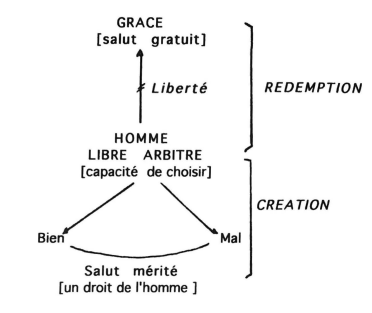
\includegraphics[width=\textwidth]{CoursTheo/Images/Augustin - Redemption.png}






A ce naturalisme, Augustin défend la thèse de la grâce. Dès 414, il entreprend de réfuter le livre de Pélage sur la «nature humaine». Il insiste sur deux aspects:

-	Une		nature	blessée.	Alors que Pélage insiste sur la bonté de la nature humaine, pensant ainsi rendre hommage et justice à son «créateur», Augustin lui reproche d'oublier que cette nature est blessée par le péché, ce qui la rend incapable de faire le bien sans l'intervention du «rédempteur».		Voici comment Augustin s'exprime :	«Mais, quand il (Pélage) croit servir la cause de Dieu en défendant la nature, notre auteur ne remarque pas qu'en déclarant cette nature saine, il évince la miséricorde du médecin...Or, nous ne devons pas louer le créateur de façon à nous trouver réduits à avouer que le sauveur est inutile.66»	Augustin n'ignore pas le libre arbitre, mais le pouvoir de choix ne devient efficace que s'il est d'abord libéré.

-	La nécessité du rédempteur. Alors que Pélage développe une théologie de la création, Augustin se fait le champion d'une théologie de la rédemption. Alors que Pélage met l'accent sur la liberté humaine, capable de choisir entre le bien et le mal, et donc capable de mériter son salut, Augustin estime que la liberté étant aliénée, elle ne devient capable de faire le bien que si d'abord elle a été restaurée dans son pouvoir
es Isabelle BOCHET, Saint Augustin et le désir de Dieu. Et. aug. , 1982, p. 320.
ee De natura et gratia 34, 39, in BA 24. Ppour une présentation d'ensemble, voir Paul Agaësse, L'anthropologie chrétienne selon saint Augustin. Image, liberté, péché et grâce. Centre Sèvres, Paris, 1980.
28	(
 
de,.1e faire. Or, étant donné le péché originel, seul Dieu peut redonner à l'homme ce qu ''· a perdu. If n'est donc pas légitime de s'attribuer à soi-même un quelconque ménte. Toute notre justification nous vient de Dieu et le salut est un don gratuit que nul n'a mérité par soi-même. "Tous ont péché" (Rm 5, 18), ce qui signifie que "personne n'est justifié si le Christ ne le justifie"67   Seule la foi dans le Christ rédempteur peut sauver l'homme, «la foi en Jésus Christ fait homme, la foi en son sang, la foi en sa croix, la foi en sa mort et en sa résurrection !88 » Il n'y a donc pas à hésiter sur la nécessité absolue de la grâce dans la condition de l'homme pécheur :
«Reconnaissons que la grâce est nécessaire; crions : Malheureux homme que je suis! qui me délivrera de ce corps qui me voue à la mort? Et que l'on réponde: la grâce de Dieu, par Jésus-Christ notre Seigneur.18 »

Quel est l'enjeu du débat ? Regardons d'abord la thèse	de Pélage. En gros, Pélage insiste fondamentalement sur la valeur de l'homme. A la création, Dieu a donné à l'homme la liberté et la raison, donc la possibilité d'exécuter volontairement le dessein de Dieu et donc de mériter par lui-même le salut. C'est une théologie de l'autonomie humaine, marquée au coin d'un certain naturalisme et d'un certain rationalisme. Pélage vantait les capactiés de la nature humaine. Cet optimisme au sujet des capacités de l'homme devait le conduire	à précher un volontarisme moral . L'homme pélagien est un être "sans reproche" :

« Ce n'est pas grand-chose, disait-il d'être un exemple pour les païens...Ce qui est beaucoup mieux, c'est d'être tel que les saints eux-memes soient édifiés.» (Cf. E.U.)

En face de ce naturalisme, qui menaçait de dévaloriser la grâce, Augustin réagit vivement en défendant la thèse de la grâce. Alors que Pélage insiste sur la bonté de la nature humaine, pensant ainsi rendre hommage et justice au "créateur" de cette nature, Augustin lui reproche d'oublier que cette nature a été blessée par le péché, ce qui la rend incapable de faire le bien et nécessite l'intervention du "rédempteur" et de la grâce. Voici comment Augustin s'exprime:

« Mais, quand il croit servir la cause de Dieu en défendant la nature, notre auteur ne remarque pas qu'en déclarant cette nature saine, il évince la miséricorde du médecin...Or, nous ne devons pas louer le créateur de façon à nous trouver réduits à avouer que le sauveur est inutile.» (De natura et gratia 34, 39, BA 24).

A l'arrière-plan de ce débat, on distingue à la fois deux  expériences différentes.

-	L'expérience d'Augustin est celle d'un converti qui s'est heurté à ses propres limites et pour qui sa conversion est l'expérience fondatrice de sa propre pensée. Le mouvement premier d'Augustin est toujours l'action de grâce pour ce que Dieu a fait de sa vie. Comme l'a bien noté G. Greshake : «Il est impossible, dans la prière, de se présenter à Dieu et de lui dire : Je dois mon salut à toi et à moi, à ce que tu as fait et à ce que j'ai fait. Dans la confessio, on peut dire seulement : ce que j'ai, je



67  De natura et gratia 41, 48.
88 lb. op. cit. 44, 51.
av Rom 8, 24-25, ib. op. cit. 53, 61.
29
 
te ledois.7»0	li dira encore : «Tu es miséricorde, je suis misère.» (Conf. X, 28, 39).	(

-  Pélage nous est  trop peu  connu pour savoir à quelle expérience pers n elle    e réfère. Ce qui est sûr, c'est qu'il représente un type de chnst,anisme qui fait appel en priorité non pas à la grâce, comme Augustin, mais aux capacités de l'homme.

\subsection{Nouvelle vague : les moines d' Adrumète et Julien d'Eclane}
 

Le jeu n'était donc pas calmé avec la condamnation de Pélage. Une nouvelle phase	Cela
allait se produire,	provoquée soit par certains disciples trop dociles d'Augustin, tels
les	moines du couvent africain d'Adrumète (Sousse, au Sud de Carthage), ou au
contraire par des disciples de Pélage, tel Julien d'Eclane.

- Les moines d' Adrumète répandirent, vers 425-426, l'idée que, puisque Dieu fait tout, la liberté n'est rien et n'a rien à faire. Prenant trop à la lettre certaines affirmations d'Augustin sur la grâce, ils en tiraient que la liberé est inexistante. Alors que les Pélagiens niaient la grâce au nom de la liberté, à l'inverse, ces moines défendaient «la grâce de Dieu jusqu'à nier le libre arbitre de l'homme». Augustin leur fit savoir que \sn{10 G. GRESHAKE, Geschenkte Freiheit. Einführung in die Gnadenlehre, Freiburg, 1977, p.
47.	Cité par Goulven MADEC, Pélage et Augustin. Le débat sur la liberté et la grâce.
Itinéraires augustiniens 13 (janvier 1995).}
\begin{quote}
    «confesser la grâce comme il l'avait fait, ce n'était pas nier le libre arbitre ni le mérite...» 
    \end{quote}
    
    Il écrit  à  Valentin, abbé du monastère :	
    \begin{quote}
        

 « Certains parmi vous exalteraient la grâce au point de nier le libre arbitre de
 l'homme, et, ce qui est plus grave, soutiendraient qu'au jour du jugement Dieu n'aura
 pas à rendre à chacun selon ses oeuvres...» (p. 53)	
«S'il n'y a pas de grâce divine, comment Dieu sauve-t-il le monde ? Et s'il n'y a	 pas de libre arbitre, comment juge-t-il le monde ?...Ne niez pas la grâce de Dieu, et
 ne défendez pas le libre arbitre jusqu'à le rendre indépendant de la grâce de Dieu,
comme	si nous pouvions sans elle concevoir	ou	accomplir quelque chose	selon	Dieu \sn{" De gratia et libero arbitrio. B.A. 24, p. 55. "Il en est qui défendent la grâce de Dieu
jusqu'à nier le libre arbitre de l'homme".	}     » (p.  SS)
    \end{quote}
 
Augustin invite à tenir ensemble les deux vérités : le libre arbitre	et la grâce. Il énumère alors une série d'affirmations tirées de l'Ecriture, les unes en
faveur de la grâce, les autres en faveur du libre arbitre. Si l'on ne peut pas	comprendre comment les deux s'articulent, il faut s'en tenir à l'Ecriture qui les
affirment simultanément \sn{B.A 24 p. 276 cf. aussi B.A. 73 B : page 480, la grâce et la liberté, et p. 477 ,
préscience divine et liberté humaine.}: 
\begin{quote}
    "Elle nous enseigne à la fois la réalité du libre arbitré · humain et la réalité de la grâce divine; grâce sans laquelle le libre arbitre ne peut ni se tourner vers Dieu ni progresser en Dieu.» (p. 59). 

\end{quote}

Y a-t- il une coordination possible des deux termes ? Augustin donne à la grâce une extension telle qu'elle englobe la liberté. La liberté est déjà grâce. La formule la plus parfaite pour exprimer le lien
entre les deux se trouve dans le "De correptione et gratia"  :	 
\begin{quote}
   «Aguntur  enim  ut	agant,  non  ut	ipsi nihil agantl» (11,  4)
«Ils sont en effet	agis pour agir, non pour ne rien faire» 
\end{quote}


-  Avec  Julien d'Eclane, le défenseur  de la liberté, le combat allait prendre une tournure plus dure. Julien invoquait à l'encontre d'Augustin un certain nombre de textes  sur la liberté - en fait sur le libre arbitre - que celui-ci avait écrits autrefois. Augustin sera obligé de rétablir ainsi l'équilibre, mais en mettant de plus en plus l'accent sur la grâce, si bien qu'on peut parfois se demander s'il réussit encore à reconnaître la place de la liberté. Il tire de !'Ecriture une série d'affirmations, les unes en faveur de la grâce, les autres en faveur du libre arbitre. Si l'on ne peut pas comprendre comment les deux s'articulent, répond Augustin, il faut s'en tenir à !'Ecriture qui les affirment simultanément : «Elle nous enseigne à la fois la réalité du libre arbitre humain et la réalité de la grlce divine; grlce sans laquelle le libre arbitre ne peut ni se tourner vers Dieu ni progresser en Dieu.»

L'affrontement entre Augustin et Pélage se joue sur l'idée que l'un et l'autre se font  de la liberté. Pour Augustin, le libre arbitre n'est pas la liberté, mais il est  la simple capacité de choisir,  de disposer librement de sa propre volonté.
« Notre volonté ne serait même plus volonté si elle n'était en notre pouvoir. Mais puisqu'elle est en notre pouvoir, elle est libre pour nous; car ce qui n'est pas libre pour nous, c'est ce qui n'est pas en notre pouvoir; et ce qui l'est ne peut pas ne pas être libre.73» Pélage n'a aucune peine à accepter cette définition. li la tirait même à lui pour démonter que Augustin n'était pas toujours Augustin, c'est-à-dire le champion intransigeant de la grâce. Seulement, alors que pour Pélage, le libre arbitre, confondu avec la liberté, est la capacité de l'homme à choisir entre le bien et le mal, pour Augustin, il se restreint  à la responsabilité de l'homme dans le mal : Il est la
«facuitas peccandi» (1, 16, 35).  Il est rare qu'il fasse appel au libre arbitre dans le choix du bien74   L'orientation vers le bien relève de· la liberté, la  «vraie»  liberté se manifestant dans la soumission à Dieu et n'existant que par la grâce. Or, la liberté qui s'est perdue en raison du péché, est incapable de se réenraciner dans le bien. Pour agir de nouveau selon Dieu, il faut une restauration de la liberté par la grâce. Pélage qui ne connaissait que le libre arbitre ne réalisait pas que, sans la grâce, donc sans la vraie liberté,  le libre arbitre était une serf-arbitre.

Si l'on voulait entrer plus avant dans ce débat, il faudrait évidemment évoquer le problème  de  la  prédestination, qui vient se greffer sur celui de la liberté. Puisque la liberté de l'homme n'est rien sans la grâce, n'est-elle pas une pure illusion, totalement régie de l'extérieur par une autre liberté, celle de Dieu, qui donne ou refuse sa grâce avant tout mérite de l'homme? C'est cette thèse que soutiendront les jansénistes, dont on reparlera. Augustin est moins radical. Mais ses propos sont souvent ambigus, sinon choquants 75   La polémique l'a parfois entraîné dans certains

73 Sur le libre arbitre 111, 3, 8. Cf. G. Madec, Itinéraires augustiniens 13 (janvier 1995.
H Cf. Enchiridion XXVIII, 106. «Car si le péché dépendait du libre arbitre seul, cependant, pour conserver la justice, lelibre arbitre ne suffisait pas si la la participation du bien immuable ne lui assurait le secours divine.»
H Cf. Enchiridion XXIII, 93. BA 91 p. 269 : «Bénigne entre toutes,à ne pas douter, sera la peine de ceux qui au péché qu'ils tenaient de leur origine se gardèrent d'en ajouter aucun.» Cette thèse a été exacerbée par les jansénistes et les calvinistes, qui ont introduit l'idée d'une prédestination négative, Dieu décidant arbitrairement, d'avance et de façon absolue, de
la destinée éternelle de chaque être.
31
 
dé pages, par exemple lorsqu'il écrit, à propos des vertus des païens, qu'elles ne sont	(
qu enflure et orgueil et, on doit, à ce titre, les regarder, non comme des vertus, mais
comme des vices»76 ; ou à propos des enfants non baptisés, lié au problème de la Prédestination, qui sont à jamais exclus de la béatitude, même si leur peine est
atténuée. La prédestination est un mystère qui renvoie à l'insondable volonté de Dieu. Si Augustin n'a pas toujours la formule équilibrée de ce mystère, puisque la volonté de Dieu est, d'une part «que tous les hommes soient sauvés», mais que d'autre part
«beaucoup plus grand est le nombre de ceux qui ne le sont pas», il refuse cependant toujours les excès auxquels certaines de ses formules se prêtaient77  L'exemple de la prédestination est le plus significatif. Augustin s'interdit de l'enseigner comme s'il s'agissait d'un fatalisme, réduisant à néant la liberté78 

S. Plaidoyer  en faveur de la grâce71

Augustin ne prétend pas avoir une théologie personnelle. Son unique livre de théologie est !'Ecriture. C'est pourquoi, il faut voir sur quels textes il appuie l'absolu de la grâce dont il se fait le champion face aux Pélagiens . Je voudrais citer quelques textes clefs qui lui servent à appuyer ses affirmations sur la grâce«>

a.	"Qu'as-tu que tu n'aies reçu... Et si tu l'as reçu, pourquoi t'en faire gloire comme si tu ne l'avais pas reçu ?" (1 Co 4, 7). Et voici le commentaire :

« C'est principalement ce témoignage de /'Apôtre qui m'a convaincu moi-même, quand j'étais dans une erreur semblable à celle de nos frères - il s'agit des moines de Provence - et je m'imaginais que la foi, par laquelle nous croyons en Dieu n'est pas un don de Dieu, mais que nous l'avons de nous-mêmes, et que nous obtenons ainsi par elle les dons divins qui nous permettent de 'vivre en ce monde avec modération' (Tit 2, 12). Je ne voyais pas que la foi est précédée en nous par la grâce de Dieu, pour que par elle nous soit ensuite donné ce que nous demandons utilement...»(De praedestinatione sanctorum 3, 7, B.A. 24 p. 479)
«La foi elle-même figure parmi les dons divins qui nous sont dispensés en ce même Esprit. Ces deux choses : croire et agir, sont nôtres en raison de notre libre arbitre, et cependant l'une et l'autre sont données par /'Esprit de foi et de charité. Car ce n'est pas la charité seulement, mais, comme il est écrit, "la charité avec la foi qui descend de Dieu le Père et du Seigneur Jésus-Christ" (Eph 6, 23).(ib. 3, 7, p. 481-483)





18 Cf. Cité de Dieu XIX, 25, . BA 37, p. 165-167, et p. 761, avec d'autres références p. 957. J. WANG TCH'ANG-TCHE, Saint Augustin et les vertus des païens. Beauchesne, 1938.
11 Enchiridion XXIV, 97 s.
78 Voir par exemple : De dono perseverantiae, 22, 57, BA 24, p. 741, et autres référence page 859. Augustin précise «la manière dont il convient d'enseigner la prédestination», insisitant sur le fait qu'on doit éviter de la présenter «de façon à la rendre odieuse».
79 Voir le dossier scripturaire dans Sesboüé, op. cit. p. 167.
8°Ces textes ont été sélectionnés par Jacques Pintard, Le docteur de la grâce, in Augustin, le
message de la foi, DDB, 1987, pp. 119 sv.:


32
(
 
b.	"Personne ne peut venir à moi si le Père qui m'a envoyé ne l'attire" (Jo 6, 44) "Magnifique éloge de la grâce! Nul ne vient s'il n'est tiré..." (26, 2, BA. 72, p. 487). Aussi est-ce juste de glorifier Dieu pou les mérites : "Lo!"5que tu couronn s leurs mérite tu couronnes tes propres dons. (Lettre 194, à Sixte, 19). Augustm illustre un u plus loin sa pensée par une comparaison cet attrait qu'exerce le Père
pour l'attacher au Christ :
«Donne-moi quelqu'un qui aime, et il sentira la vérité de ce que dis. Donne-moi un homme tourmenté par le désir, donne-moi un homme en marche dans ce désert et qui a soif, qui soupire après la source de l'éternelle patrie, donne-moi un tel homme, il saura ce que je veux dire.» (lb. 26, 4, pp. 491-493).
«Tu montres  un rameau vert à une brebis, tu l'attires. On présente des noix à
un enfant, il est attiré...Si donc ce qui est révélé des délices et des voluptés terrestres à ceux qui les aime les attire, ...comment le Christ révélé par le Père n'attirerait-il pas ? » (ib. 26, s, p. 497).
c.	"Dieu résiste aux orgueilleux et donne sa grâce aux humbles" (Proverbes 3, 34, et cité en I P 5, 5 et Jac 4, 6). Augustin cite SS fois cette sentence dans son oeuvre, selon la comptabilité de La Bonnardière. Elle indique qu'il n'y a pas d'autre voie vers Dieu que l'humilité du Verbe.

Augustin, on l'a vu, fut profondément marqué par cette découverte du Christus humilis. Le grand obstacle à la rencontre de Dieu est l'orgueil: "Dieu s'est fait humble, et l'homme est orgueilleux" (Sermon 142, 6)

d.	"Donne ce que tu commandes et commande ce que tu veux" Da quod jubes et jube quod vis ! (Conf. X, 29, 40; 31, 45; 37, 60). Augustin lui-même rappelle combien cette sentence avait irrité Pélage. Il écrit dans le De dono perseverantiae :
\begin{quote}
    « Parmi mes ouvrages, en est-il un qui ait été plus répandu et plus goûté que mes Confessions ? Or, dans cet ouvrage, publié lui ausi avant que n'eût paru l'hérésie pélagienne, je dis, et plusieurs fois à notre Dieu :"Donnez ce que vous commandez et commandez ce que vous voudrez." Ce sont ces paroles de moi que Pélage, à Rome, entendit un jour citer par un de mes frères et collègues dans l'épiscopat; il ne put les supporter, et dans l'émotion vive qu'il mit à les contredire, peu s'en fallut qu'il se prit de querelle avec celui qui les avait rappelées. Mais qu'est-ce que Dieu nous commande d'abord et par dessus tout, sinon de croire en lui ? Donc, c'est lui qui nous donne de croire..." (B.A. 24, 20, 53)
\end{quote}


\begin{quote}
    L'espérance ne déçoit point, parce que l'amour de Dieu a été répandu dans nos co ur par le Saint-Esprit qui nous fut donné" (Rom 5, 5). 
\end{quote}
Un verset qui est cité pas moins de 200 fois. Augustin précise:
\begin{quote}
    « · Quand nous disons que Dieu aide à accomplir toute justice et opère en nous le vou o r et le faire (cf. Ph 2, 13) ... ce n'est pas parce qu'il fait ressentir en nos sens xt ieurs les préceptes  de la justice, mais parce qu'il donne l'accroissement mt neur   I Co 3, 7), en répandant la charité dans nos coeurs par /'Esprit-Saint
qw nous a ete donne» (L'esprit et la lettre 25, 42)

\end{quote}

 
 
Loin de contredire le libre arbitre, la présence de !'Esprit le dégage au contraire	( pour le rendre libre : "Partout où est !'Esprit du Seigneur, là est la liberté (2 Co 3,
17, là, le coeur humain est dilaté, ce qui fait dire à Augustin : « Cet Esprit de Dieu dont
la présence nous justifie, nos inspire la haine du péché et nous donne la liberté spirituelle» (ib. 16, 28).

\subsection{Nouveaux	rebondissements sur liberté et	grâce}
 

La thèse de la prédestination rebondit plusieurs fois au cours de l'histoire. Qu'il suffise de donner quelques points de repères. Trois moments, de plus ou moins d'ampleurs, on marqué ce débat.

a)	La question rebondit une première fois au IXe siècle, avec les thèses d'un moine, Gottschalk\sn{81 Cf. Kurt FLASCH, Introduction à la philosophie médiévale, Cerf, Ed. universitaires de Fribourg, 1992, p. 29 s., en particulier p. 33 s. sur Godescalc et la prédestination divine.} , fils d'un prince saxon, qui vivait au monastère d'Orbais (diocèse de Soissons). D'un esprit étroit, il enseignait que Dieu prédestine aussi bien les damnés à l'enfer que les élus au ciel. L'idée même de prédestination absolue entraîne aussitôt chez Gottschalk la négation de la liberté. De plus, introduisant I' idée d'une prédestination négative, il transforme Dieu en monstre, puisqu'il devient l'auteur du pire mal qui puisse arriver à l'homme. Inutile d'ajouter que, dans ces conditions, la rédemption laisse totalement hors de son champ ceux qui sont d'avance exclus du salut.

Cette théorie monstrueuse, qui se prétend l'expression de la pensée d'Augustin, sera condamnée : le concile de Valence (855) réaffirmera l'universalité du salut et la rédemption de tous, en même temps qu'il rcconna1t .; tout homme la liberté et le pouvoir de se sauver. Durant le Moyen Age, c'est cet augustinisme tempéré qui va s'imposer. Sans rien enlever à l'absolu de la grâce, les scolastiques partiront de l'idée de l'universalité du salut, une doctrine qui était passée quelque peu sous silence, et le reste, c'est-à-dire grâce et liberté, y est subordonné. Pour sauver les hommes, Dieu n'est pas tenu par les sacrements, dira saint Thomas. Il dispose de bien d'autres moyens.

b)	Avec  la  Réforme,  la  question  deviendra  beaucoup  plus  aiguë. Luther et Calvin se réclament tous les deux d'Augustin. De tous les auteurs anciens, Augustin est à leurs yeux le meilleur interprète de !'Ecriture. «Augustinus  meus totus est», déclare Luther dans sa polémique avec Erasme : «De ton côté sont les théologiens modernes et tant d'universités, de conciles, d'évêques, de papes! ...De mon côté, au contraire, seulement Wyclif et Laurent Valla, mais aussi Augustin, que tu passes sous silence, m'appartient tout entier.» De même, Calvin se place sous l'autorité  d'Augustin,  qu'il  cite  341  fois  dans  la  seule  Institution  chrétienne.
«Augustinus totus noster est», écrit-il en écho à Luther : «Quant à saint Augustin, il s'accorde si bien en tout et partout avec nous, il est tellement nôtre (adeo totus noster est) que s'il me fallait écrire une confession sur cette matière, il me suffirait de la composer des témoignages extraits de ses livres... Je ne dis rien qu'il n'ait dit devant moi mot à mot.» Si l'on considère ce qui a séduits les Réformateurs, c'est, on s'en doute, la doctrine augustinienne de la grâce et de la justification. Chez Calvin, c'est toujours dans le contexte de sa défense de la prédestination qu'il cite Augustin, sans
s'apercevoir que l'idée d'une double predestination, le salut pour les uns et la J>erdation Pour les autres, dont il se fait le défenseur, est totalement étrangère à Augustin\sn{82 Cf. Augustinus Magister. Etudes augustiniennes, 1954. Il, 1029 s. pour Luther et saint Augustiin (Léon Cristiani), et 11, 1839 s. pour Calvin et saint Augustin (Jean Cadier).
63 Léon CRISTIANI, Luther et saint Augustin, dans Augustinus Magister Il, 1954, p. 1037 -1038.
84 Cf. Henri de LUBAC, Augustinisme et théologie moderne. Aubier, 1965, p. 15 s.}

Quand en effet on y regarde de plus près, on s'aperçoit que, au-delà de l'appel explicite à son autorité, Augustin ne sert chez Luther et Calvin qu'à cautionner des thèses qui sont les leurs plus que les siennes. Cet a priori de lecture est évident chez Luther. Alors même qu'il se croit dans la ligne d'Augustin, il oublie des pans entiers de sa pensée. En particulier, sa thèse sur la justification ne saurait être tirée d'Augustin sans autre forme de procès. Augustin ne dissocie jamais foi et charité. Alors que Luther soutient que la foi seule justifie, Augustin dit que c'est la charité dans son obéissance à la loi. Luther n'a d'ailleurs pas été sans lui-même relever cet écart. Mais au lieu de rectifier sa propre position, il accuse Augustin d'inconséquence ou d'infidélité à lui-même. Melanchton, avec l'accord de Luther, avouera explicitement à Brenz : Augustin, qui avait d'abord nié que l'homme puisse être justifié par lui­ même devant Dieu, «imagine ensuite que nous sommes réputés justes en raison de l'accomplissement de la loi que le Saint-Esprit opère en nous... Augustin n'est pas en accord complet avec la doctrine de saint Paul, bien qu'il en approche davantage que les Scolastiques... » Il ajoute que, pour le public, il faut continuer à invoquer l'appui d'Augustin, «bien qu'il n'explique pas assez la justice par la foi»83 

c)	Le	jansemsme	représente	le	troisième	rebondissement.	Sa préhistoire commence avec Michel Baius (1513-1589), chancelier de l'université à Louvain, qui avait fait d'Augustin son cheval de bataille contre les protestants. Il avait lu, nous dit-on, neuf fois tout saint Augustin et soixante-dix fois les écrits sur la grâce f Ce qui ne l'a pas empêché de se fourvoyer sérieusement. Le point névralgique de sa position tourne autour du rapport entre nature et grâce. Dans l'état initial d'Adam, la «nature» de l'homme était dotée d'une puissance autonome en face de Dieu, c'est-à­ dire d'une liberté capable par elle-même de faire son salut, si bien que si l'homme était fidèle à sa nature, il pouvait en droit prétendre à la récompense. «Chez l'homme d'avant la chute, la vie éternelle... n'aurait pas été un don de la grâce, mais un salaire.» C'est la thèse de Pélage : «Dieu me fait homme, mais c'est moi qui me rend juste», sauf que Baius parle de la condition de l'homme	d'avant la chute, tandis que . Pélage parle de sa condition actuelle .

On a dit de Baius qu'il était un «Pélage  du  paradis  terrestre». Depuis la chute, en effet, la grâce est devenue indispensable à l'homme, comme un ajout extérieur à une nature blessée et déficiente, alors qu'elle ne l'était pas avant. En se voulant fidèle à Augustin, Baius en fait le trahit, car pour Augustin,aussi bien dans l'état primitif que dans l'état actuel, sans la grâce, l'homme est incapable de parvenir au salut. Adam, pas plus que l'homme déchu, ne peut s'attribuer à lui-même un quelconque mérite.  	Au fond, Baius n'a sauvé Augustin qu'au prix d'une double déformation, à la fois du concept de nature et du concept de la grâce. Au regard de la pensée d'Augustin, l'extrinsécisme de Baius est une aberration. Mais la question se pose aussitôt : Baius, qui a été condamné, n'aurait-il pas entraîné dans sa chute Augustin lui-même? C'est ce que prétendaient certains jésuites.


 
C'est pour réfuter cette prétention que Jansénius (1585-1638), fu ur évê ue d'Ypres, rédige un ouvrage de synthèse sur la pensée d'Augustin : I' Augustmus qui ne sera publié qu'après sa mort, en 1640, et dont les jansénistes eront leur Bible. De Jansénius aussi, on nous dit qu'il avait lu «dix fois saint Augustm, et plus d? tren e fois les ouvrages de la grâce contre les Pélagiens», ce qui ne l'empêche pasd aboutir, en fin de compte, à une «consciencieuse méprise». En réalité, il ne fait que prolo,nger Baius, mais en l'inversant. Alors que Baius part d'une nature qu1, au moms dans I état d'Adam, peut prétendre au salut, la grâce devenant inutile, Jansénius part de l'absolu de la grâce, expression de la puissance arbitraire de Dieu, qui la donne ou la refuse sans tenir compte de l'homme, pour refuser ensuite à la nature humaine, d nc à la liberté, toute consistance propre. «Si l'un et l'autre tendent également à dissoudre l'union entre Dieu et l'homme en quoi consiste essentiellement le Mystère du Christ, écrit le P. de Lubac, n'est-ce pas que l'un dresse l'homme en face de Dieu dans la réclamation de ses droits, tandis que l'autre l'anéantit ?fJS »
La thèse de Jansénius sera à l'origine de tous les débats modernes autour de la grâce, dont Port-Royal,  avec l'abbé de Saint-Cyran à sa tête, sera le foyer en France. Délaissant les spéculations de Baius sur l'état primitif de l'homme, tout comme celles de Jansénius sur la «pure nature», Saint-Cyran s'intéresse à l'homme concret, pour le placer d'emblée devant le mystère redoutable de la grâce, une grâce rare, qui n'est donnée qu'à un petit nombre d'élus. «Comme le soleil fait des jours sacrés et des jours profanes, des jours de fête et des jours civils, des jours d'été et des jours d'hiver, ainsi Dieu a fait certains hommes pour être sauvés et saints, et d'autres profanes pour être damnés... ». «li ne tombe pas une goûte de grâce pour les païens !» Saint-Cyran, sans lequel le jansénisme n'aurait sans été qu'une «hérésie de professeurs», lui assurera le succès. Mais c'est bien à tort qu'il invoque saint Augustin. A aucun moment, Augustin n'a pensé que le destin de l'homme pouvait être scellé de l'extérieur par Dieu, sans que la responsabilité de l'homme y soit engagée. Alors que les débats sur la grâce et la prédestination, tels qu'ils se sont développés dans le jansénisme, se placent au point de vue de l'éternité, où tout semble joué d'avance, Augustin considère l'homme dans son devenir temporel, où l'alternative entre la lumière et les ténèbres reste toujours ouverte86 

\section{Conclusion}
\begin{Synthesis}
 Augustin maintiendra contre vents et marées le primat de l'action de Dieu. Il n'a pas réussi à concilier par des concepts l'action de Dieu et l'agir de l'homme. Le champion de la liberté contre les manichéens s'est battu avec la même i tran igeance en s faisant le champion de la grâce contre les Pélagiens. Augustin s'en tient a la parole de l'Ecriture, faisant siennes ce texte de l'Apôtre: .
\begin{quote}
    «  Qui es- tu pour discuter avec Dieu ? (Rm 9, 20)  Impénétrables  sont ses Jugements et incompréhensibles ses voies (Rm 11, 33) Et il ajoute : "Ne cherche pas a atteindre ce qw est trop haut pour toi, ni à scruter ce qui te dépasse"» (Ecc 3, 22) (De Dono perseverantiae XII, 30, B. A. 24 p. 669)
\end{quote}
\end{Synthesis}




Au cours des siècles, cette doctrine de la grâce fut tirée vers une doctrine intolerable, celle de la prédestination, et en particulier de la prédestination négative, notamment chez les Jansenistes et les calvinistes. Dieu est alors un Dieu arbitraire,
pervers, qui décide d'avance, de façon absolue, qui va au ciel et qui va en enfer, indépendamment des mérites :
\begin{quote}
    « Par décret de Dieu, et pour la manifestation de sa gloire, tels hommes sont prédestinés à la vie éternelle, tels autres voués à la mort éternelle!» (Confession de Westminster, 1647).
\end{quote}


Une telle doctrine n'est pas augustinienne, même si certaines formules peuvent être tirées en ce sens. Mais il faut bien constater que ce sont ces excès modernes qui furent à l'origine d'une certaine forme d'athéisme, l'athéisme humaniste, qui oppose Dieu et l'homme, la grâce et la liberté, et qui rejette Dieu au nom de l'homme et de la liberté.
\begin{quote}
    "M'en coûtât-il d'être expédié en Enfer, disait Milton, jamais un tel Dieu ne m'imposera le respect!" (Cf. Max WEBER, L'éthique protestante et l'esprit du capitalisme, Pion, p. 117.)
\end{quote}"M'en coûtât-il d'être expédié en Enfer, disait Milton, jamais un tel Dieu ne m'imposera le respect!" (Cf. Max WEBER, L'éthique protestante et l'esprit du capitalisme, Pion, p. 117.)

Augustin était trop conscient de la liberté de l'homme pour croire qu'elle pouvait être mise en échec par la grâce. Celle-ce n'est pas contre la liberté, ni au-dessus de la liberté, mais avec la liberté qu'elle rachète et rend efficace dans l'ordre du salut. L'acte le plus libre est celui par lequel l'homme accepte de reconnaître que tout lui est donné, y compris sa liberté.
 
























37

%

% \chapter{Lire les classiques Chinois}

 

\textbf{Comment lire les classiques chinois ? (French Edition)}

\textbf{Vermander, Benoît}

\section{Prologue}


\subsection{Période axiale}
  \mn{ p. 5 · E. 59  } \begin{quote}
Lorsque la notion même de « période axiale » est acceptée au moins comme
hypothèse de travail ( elle est parfois rejetée dès l'abord ) , les
percées qu'on lui associe sont généralement les suivantes : ( a ) les
penseurs de la période auraient contribué à « problématiser le monde »
plutôt qu'à le recevoir tel quel , ce par le fait d'articuler la réalité
sociale autant que naturelle autour de questions portant sur son «
pourquoi » et son « comment » ; ( b ) c'est ainsi qu'aurait émergé la «
conscience critique » , l'examen des opinions reçues , la remise en
cause d'au moins certaines des structures sociales ; ( c ) ce
questionnement
aurait nourri un souci éthique ( à moins que ce dernier ait contribué à
l'émergence de la conscience critique ) , souci qui fut accompagné
souvent de la formation d'une vision utopique -- la cité idéale de
Platon , la pleine libération des individus dans le bouddhisme , le rêve
d'un ordre social gouverné par les rites , l'éducation morale , chez
Confucius , l'annonce de la venue du Royaume de Dieu chez les prophètes
d'Israël ; ( d ) le surgissement critico - éthique aurait été porté par
des personnalités incarnant les « sauts » entrepris , personnalités dont
le nom est transmis aux générations qui leur succèdent ; ( e ) ces
personnalités sont souvent représentées ( et semblent s'être considérées
elles - mêmes ) comme des « Renonçants » , des individus dont les choix
de vie mettent en question l'ordre dominant : dans la République , le
philosophe de la cité idéale de Platon renonce aux possessions privées
et à la vie de famille pour gouverner la Cité avec justice

\end{quote}  

\subsection{Divination, mathématique et concepts}
\mn{- p. 17 · E. 258  } \begin{quote}  

Élaborer des ramifications entre les principaux viscères du corps humain
et les états climatiques ( le chaud , le froid , le sec , l'humide ) ,
les émotions , les notes de musique , les couleurs , tout cela transcrit
dans une arithmétique de
base cinq » , n'est pas simple opération de l'esprit mais permet bien
d'observer pragmatiquement un ensemble de correspondances . En même temps, ces analogies deviennent moralement signifiantes. C’est ainsi que s’opère une évolution du divinatoire au combinatoire et à l’éthico-politique.   
A la fois matrice de ce processus et l'accompagnant tout au long de sa
formation textuelle , le \textit{Classique des mutations ( Yijing )} construit un
métalangage de l'univers à partir d'une réflexion mathématisée sur les
processus de divination.
il s'essaie à décrire la façon dont les phénomènes se suivent et
s'agencent de façon nécessaire . C'est , à l'extrême , une mathématique
de tous les phénomènes possibles , fondée sur l'idée que tout n'existe
que dans l'échange , le passage , la fluidité : la gradation est un
autre nom du contraste , et la logique des transformations ( des
changements par quoi une forme entre en contraste avec celles qui la
précèdent et la suivent ) , non pas celle des oppositions , régit
l'univers et la pensée .

\end{quote} \mn{ p. 18 · E. 268 } \begin{quote}

Au ciel se composent les images {[} xiang {象} {]} , sur la terre se
composent les formes {[} xing 形 {]} , et les transformations se font
visibles {[} Yijing , Xici 繫辭 I . 1 {]} 28 .

\end{quote} 

\paragraph{le rite comme éducation} chez Confucius
\mn{p. 20 · E. 304  } \begin{quote}

Le vecteur de l'éducation ainsi dispensée , ce sera le rite
: l'éducation de l'intérieur par l'extérieur . À noter pourtant que « le
rite » ( chinois ) et « la loi » ( en contexte grec ou hébreu ) ne se
trouvent pas dans un strict régime d'opposition : ils régulent tous deux
les conduites extérieures jusqu'au moment où les prescriptions se
retrouvent être inscrites « au fond des cœurs » .

\end{quote} \mn{ p. 24 · E. 367 } \begin{quote}

La détermination d'un corpus de classiques fonde une culture dans sa
spécificité tout en lui donnant d'affirmer son l'universalité latente .
Hans - Georg Gadamer fait de l'extensibilité ,  en principe illimitée, de la durée pendant laquelle une œuvre communique son sens le trait qui désigne un « classique »
\end{quote} 
 
\section{Chapitre I : Qu'est-ce qu'un classique chinois ?}

\mn{ p. 37 · E. 786 } \begin{quote}

Du reste , dès les premiers rencontres entre lettrés chinois et
missionnaires occidentaux , les uns et les autres comprennent que le
continent qui leur fait face est fondé sur une armature de classiques
dont la maîtrise est essentielle pour la réussite culturelle ,
religieuse et sociale , et ils feront de la connaissance réciproque de
ces textes la clé d'une rencontre possible , d'une entrée dans la pensée
de l'Autre , que ce soit pour l'apprécier ou l'utiliser , pour
convaincre ou dominer l'interlocuteur .

\end{quote} \mn{p. 38 · E. 805  } \begin{quote}
On trouve cette acception chez Yang Xiong 揚雄 (53 AEC-18) :

 
 \begin{quote}
     : « Un texte qui ne se mesure pas aux Classiques n’est pas un texte. Une parole qui ne se mesure pas aux Classiques n’est pas une parole. Ce sont des excroissances qui prolifèrent  
 \end{quote}
La formule, très concise, pourrait aussi être comprise comme signifiant : « Un texte qui n’est pas (qui ne tend pas au) Classique n’est pas un texte. » Ou même plutôt : \textit{« Un texte non référé à une norme n’en est pas un. »} Le registre sémantique du passage 11 rappelle celui qui entoure le terme déjà évoqué κανών : l’instrument qui norme (la règle du charpentier en grec) donne naissance à un ensemble textuel établi par rapport à lui – ensemble qui, de normé, devient alors normatif.
 
\end{quote} \mn{p. 44 · E. 926  } \begin{quote}

Pouvoir {[} di {]} d'en haut {[} shang {]} » surplombe le monde
surnaturel ( ne parlons pas d'un « panthéon » ,car on n’y trouve pas l’individuation des divinités qu’on attache d’ordinaire à ce terme).

 

\end{quote} \mn{ p. 45 · E. 951 } \begin{quote}

L'autre chapitre des Documents sur lequel nous nous arrêterons
brièvement est celui du Hongfan 洪 範 , expression que l'on peut
traduire par « Grand plan » ou , sans doute plus justement , par «
Modèle universel » . Il présente l'ensemble des phénomènes ( éléments ,
conduites , matières politiques , calendrier , sources de bonheur et
malheur ) sur des combinaisons fondées sur les chiffres Cinq et Neuf .
Sa composition apparaît si rigoureuse que certains formalistes russes
ont spéculé sur son nombre de caractères et leur inscription à
l'intérieur d'un carré magique 30

\end{quote} 

\paragraph{les annales historiques} attribuées à Confucius : essayer de dicerner les signes des temps. 
\mn{ p. 56 · E. 1164 } \begin{quote}
les lecteurs de ces Annales vont s’employer à faire émerger des sens, à trouver l’expression du mandat du Ciel dans cette succession d’événements qu’ils vont lire comme une sorte de rébus. C’est dire que ce sont les commentaires suscités par l’œuvre qui en font tout l’intérêt.
[..]
Au travers de la sèche prose des Printemps et
  Automnes , le Gongyang s'emploie à trouver « le sens profond de paroles
subtiles"
\end{quote}


Importance du processus de mémoire.

 \mn{p. 59 · E. 1228  } \begin{quote}

Au travers de cet hommage rendu par les historiographes du Zuozhuan à
leurs prédécesseurs se donne à lire leur conviction : l'enregistrement
et la qualification fidèles des événements sont questions de vie ou de
mort . Cela parce que l'enchaînement des actions , des prédictions que
l'on en tire , de la vérification ou non de ces prédictions constitue la
trame de l'ordre du monde , et qu'en altérer le récit , c'est forcément
en distordre la marche .

\end{quote}

\paragraph{Anectdote : matériau de la connaissance historique} car elle offre un aperçu soudain sur une réalité plus profonde et étendue, comme la citation. \mn{ p. 59 · E. 1233 } \begin{quote}
Du fait de la nature même de ces deux extraits, on aura noté la place que joue, dans le Zuochuan, le genre littéraire très particulier de l’anecdote.
 
Elle est révélatrice d'une tendance plus générale : l'anecdote , dans
l'historiographie chinoise , deviendra le matériau même de la connaissance historique.
 

\end{quote} 
\subsection{le sacrifice comme lieu de l'unité}
Une partie des textes classiques visent à expliquer la tenue en cas de non respect du sacrifice. Cette importance peut étonner.
\mn{p. 65 · E. 1345  } \begin{quote}

C'est en distinguant qu'on peut droitement unir .
Le

mode de découpe de l'animal sacrifié puis la façon dont on répartit les
parties découpées constituent des opérations destinées à symboliser et
réaliser la cohésion du groupe , dans un modèle qui associe exigence
d'unanimité et affirmation de principes hiérarchiques stricts . 

\end{quote} \mn{ p. 66 · E. 1353 } \begin{quote}
Le sacrifice
était donc image inversée de l'ordre social effectif . La supériorité
sociale était étroitement associée à la capacité de donner .

\end{quote} \mn{  p. 66 · E. 1356 } \begin{quote}

Les anomalies rituelles relevées par les textes fonctionnent alors comme
informations historiques d'importance particulière . La crise rituelle
est toujours symptôme de crise politique .

\end{quote} \mn{ p. 66 · E. 1357 } \begin{quote}

le Liji traduit une anxiété face à tous les dysfonctionnements possibles
de l'activité rituelle , et , de ce fait , du travail social .

\end{quote} \mn{p. 67 · E. 1368  } \begin{quote}

Le rituel est donc affecté par une tension entre son but avoué -- édifier ,
maintenir un ordre -- et le fait qu'il soit par essence une entreprise
risquée , soumise à divers aléas .

\end{quote} 
\subsection{La grande Etude - Daxue}
\mn{p. 67 · E. 1384  } \begin{quote}

Tentons après tant d'autres une traduction de cette célébrissime entrée
en matière -- sachant qu'aucun lecteur ni commentateur n'arrive à faire
vraiment abstraction de la lecture qu'en ont effectué Zhu Xi et ses
continuateurs . 
\begin{quote}
    La voie de la Grande Étude 96 , c'est d'éclairer {[} le
principe de {]} vertu qui {[} lui - même {]} éclaire {[} toute chose {]}
, c'est d'aimer {[} ou bien de « renouveler » , selon les versions {]}
le peuple , et c'est de ne s'arrêter qu'une fois la plus haute
perfection atteinte . Sachant le terme , on prend sa détermination . Une
fois déterminé , on peut s'apaiser {[} jing 靜 97 {]} . Une fois apaisé
, on peut s'ancrer dans la paix . Quand on est ancré dans la paix , on
peut discerner . Ayant discerné , on peut atteindre le but . Les plantes
ont racine et branches , les affaires un commencement et une fin . Celui
qui sait la succession des affaires , il est tout proche de la voie .
大學之道,在明明德,在親[新]民,在止於至善。知止而后有定,定而后能靜,靜而后能安,安而后能慮,慮而后能得。物有本末,事有終始,知所先後,則近道矣。


\end{quote}


\end{quote} \mn{ p. 69 · E. 1411 } \begin{quote}

La partie gauche du caractère , sa clé sémantique , c'est le jade ( yu 玉 )
. Associée à l'autre partie du caractère , cette clé donne à l'ensemble
un tour plus abstrait : elle parle d'une structure sous - jacente aux
phénomènes qui prennent corps . Les Chinois ont trouvé dans les nervures
du jade la plus marquante des expressions des forces vitales qui , à
l'interne , structurent l'organisme.

\end{quote} 
\paragraph{L'invariable milieu, à l'autre extremité des quatre livres}
\mn{ p. 69 · E. 1420 } \begin{quote}
Comme pour la Grande Étude, voyons à traduire le premier paragraphe du texte :
\begin{quote}
La loi du Ciel 101, c’est ce qu’on appelle « la nature » 102. Se conformer à la nature, c’est ce qu’on appelle « la voie ».
\ldots

   Aussi , l'homme de bien se tient sur ses gardes même quand il ne
distingue rien {[} d'inquiétant {]} , il craint et tremble même quand
rien ne frappe son oreille . 
 
\ldots

Aussi , l'homme de bien reste sur ses gardes {[} même {]} dans la
solitude 104 . N'émettre {[} fa 發 {]} ni joie ni colère ni tristesse ni
allégresse , c'est ce qu'on peut appeler l'équilibre {[} le milieu {]} .

\end{quote} 
\end{quote}

Relecture

\paragraph{Xunzi : la discrimination fait l’homme
 }
\mn{ p. 72 · E. 1482 } \begin{quote}

On a argué , à mon sens fort justement , que le caractère fen 分 (
séparer , diviser ) constitue une clé -- sinon la notion clé -- du Xunzi
112 . Le fait que l'on compte 113 occurrences du caractère dans
l'ouvrage est un premier signe de son importance .

\end{quote} \mn{ p. 73 · E. 1493 } \begin{quote}

le principe de base sur lequel Xunzi fonde sa théorie politique est que
les désirs ( par essence subjectifs ) sont par nature illimités , tandis
que les biens sont objectivement limités ( yu duo er wu gua 欲 多 而 物
寡 113 ) . Savoir comment répartir et partager , c'est bien là l'essence
de l'art politique 114 . Xunzi pose ici l'accent sur la notion de gong
公 : gong ( habituellement traduit par « chose publique ») consiste à diviser quelque chose avec impartialité, sans afficher égoïsme ou partialité (si 私).
 

\end{quote} \mn{ p. 74 · E. 1510 } \begin{quote}
Le rituel, manifestation privilégiée des distinctions ainsi effectuées, devient alors le conduit par quoi ce qui était au départ
de l'ordre de la nature ( xing 性 ) se transforme en artifice ( wei 偽 )
, ce dernier terme revêtant un sens éminemment positif
 
\end{quote} 
Sens positif de l'artifice chez xunxi.
\begin{Def}[artifice]

\end{Def}
\mn{ p. 74 · E. 1522 } \begin{quote}

Xunzi trace une distinction entre les niveaux atteints respectivement
par le Lettré ( shi 士 ) , l'homme de bien ( junzi 君子 ) et le sage (
shengren 聖人 ) , ce dernier seul capable de fusionner en un tout la
perfection des dispositions à l'interne et celle atteinte par les
observances extérieures .



\end{quote}


Cf vie digne et vie parfaite

\mn{p. 75 · E. 1527  } \begin{quote}

Les châtiments contribuent à assurer l'équilibre entre hiérarchie et
impartialité .

\end{quote} \mn{ p. 76 · E. 1550 } \begin{quote}

Xunzi voyait bien la nature humaine ( xing 性 ) comme mauvaise ( e 惡 )
, il discernait dans l'artifice rituel couplé à la droite éducation la
route par laquelle s'ouvrait la possibilité de dépasser l'inné , jusqu'à
rendre chacun capable de devenir -- en théorie -- semblable aux sages souverains du temps passé. Route trop dangereuse pour le Hanfeizi, quand les États font face à des risques imminents (la principauté dont Han Fei est un dignitaire éminent va disparaître trois ans après sa mort).
 
L'art politique ne consiste pas à éduquer le peuple , que ce soit par
les rites ou par la vertu , mais à instaurer un ordre durable au moyen
des châtiments et récompenses attachés à des lois valables pour tout un
chacun . Notons que
les Légalistes systématisent ici une vue politique apparue bien
auparavant , mais à laquelle les penseurs classiques avaient jusqu'alors
été à même de s'opposer : le Zuozhuan relate qu'en 536 AEC , l'État de
Zheng 鄭 fonde dans le bronze un code des châtiments . Il reçoit une
algarade d'un ministre de l'État de Jin 晉 , qui rappelle à tous que les
anciens rois comptaient , pour assurer l'ordre public , sur le rituel ,
le sens de la justice , l'attrait des positions officielles , l'exemple
donné par leur dévouement constant \ldots{} Ils savaient que l'existence
même d'un code intangible ne pouvait que corrompre la fibre morale d'un
peuple 116 . Pourtant , vingt - trois ans après cet épisode , l'État de
Jin cède à la même tentation 117 \ldots{} Nous approchons là de la fin
des récits du Zuozhuan :

\end{quote} \mn{p. 77 · E. 1580  } \begin{quote}
Ou encore comme le roi-sage taoiste,  \begin{quote}
    il
agit par le non agir ( wei wu wei 為 無為 ) 
\end{quote}, mais s'il est en mesure
de procéder ainsi c'est parce qu'il a institué l'artifice d'un corps de
loi simples , compréhensibles , adaptées au temps présent et cependant
universelles par leur inspiration , des lois qui , en quelque sorte ,
gouvernent à sa place -- pour autant qu'elles soient conformes à l'ordre
naturel : Les choses ont leur usage , les talents leur emploi . Lorsque
tout est en place , alors on n'a pas à s'activer du haut vers le bas .
Ordonnez à un coq de proclamer l'aube , ou à un rat de chasser les
souris ! {[} Hanfeizi , Yangquan , 1 {]} .

\end{quote} \mn{p. 79 · E. 1614  } \begin{quote}

Voyant un teinturier teignant la soie , Mozi dit tout en soupirant : Ce
qu'on teint en bleu devient bleu , ce qu'on teint en jaune devient jaune
. Quand on change {[} la teinture {]} dans quoi l'étoffe est immergée ,
change pareillement sa couleur . Trempée cinq fois , sa couleur
nécessairement changera cinq fois . Lorsque l'on teint , on ne saurait
être trop prudent {[} Mozi , Suoran , 1 {]} . 子 墨子 言 見 染 絲 者 而
歎 曰 : 「 染 於 蒼 則 蒼 , 染 於 黃 則 黃 。 所 入 者 變 , 其 色 亦
變 。 五 入 必 而已 , 則為 五色 矣 。 故 染 不可 不慎 也 。 」

\end{quote} \mn{p. 82 · E. 1666  } \begin{quote}

La partialité insère des négations dans une réalité de soi toute marquée
par l'affirmation . En contraste : l'attitude inclusive ( impartiale )
est toute positive :
\begin{quote}
    « Je fais pour l’autre comme pour moi-même » (wei bi wei you wei ji ye 為彼猶為己也, Mozi, Jian’ai, III, 2).
 
\end{quote}
\end{quote} \mn{p. 83 · E. 1695  } \begin{quote}

Pareille étincelle pourrait être par exemple la « découverte » faite par
Mozi que l'amour n'apporte bénéfice effectif que pour autant qu'il
s'abstienne de discriminer , de hiérarchiser . Il est plus aisé
d'imaginer que pareil basculement fut à l'origine de l'attraction
exercée par Mozi que d'y voir un développement « naturel » ( on ne voit
pas du reste en quoi il serait tel ) d'un appel initial à la simple
bienveillance .

\end{quote} 
\paragraph{des écrits pour se taire}
\mn{ p. 84 · E. 1701 } \begin{quote}

EN décalage peut - être plus grand encore que les textes mentionnés à
l'instant , dans la mesure où leurs principes épistémologiques diffèrent
profondément de ceux défendus par les lettrés ( shi 士 ) , le Daodejing
道德 經 ( ou Laozi 老子 ) et le Zhuangzi 莊子 comptent parmi les textes
les plus influents de la pensée chinoise -- et universelle .
\end{quote}
 
 
 \chapter{Rentrée ISTR 2022}

\section{Introduction }
\mn{Xavier Gué, Septembre 2022}
AU sein de la théologie de l'ICP, l'ISTR (Institut de Sciences de Théologie des Religions) affirme son intérêt sur l'autre :
\begin{itemize}
    \item clé de ces religions
    \item regard distancié 
    (Sociologie, Symbole rite des religions)
    
\end{itemize}

mais pas uniquement de la connaissance des religions. Le concile Vatican II va promouvoir un regard positif sur les autres traditions religieuses.
\paragraph{
Sorte de paradoxe de l'ISTR}
\begin{itemize}
    \item Dialogue : l'accueil des autres religions (Nostra Aetate)
    \item Annonce et mission (Ad Gentes : V2 qui promeut l'annonce)
\end{itemize}
Ce paradoxe, on pourrait l'éteindre. 

\subsection{Quelle mission pour l'ISTR}
pas seulement des informations mais modeler les personnes pour qu'elles puissent vivre heureuses dans ce monde.
Christoph Theobald \sn{sur l'alterité de l'autre}
\begin{quote}
    tacitement, on suppose que si la personne avait une connaissance interne du Christianisme, il 
\end{quote}
Il ne faut pas confondre Mission et prosélytisme.

la seconde tentation, ce serait d'absolutiser l'individualisation de l'autre. Nous tombons alors dans la privatisation de la Religion ou une tentation communautarisme.

L'institut se place dans un ni-ni : 
\begin{itemize}
    \item ni prosélytisme
    \item ni aucun rapport aux autres
\end{itemize}
Le mot serait de \textit{l'hospitalité}.  
\begin{quote}
    N'oubliez pas l'hospitalité; car, en l'exerçant, quelques-uns ont logé des anges, sans le savoir. He 13,2
\end{quote}
Dieu nous surprend.


Jésus rencontra de nombreuses personnes et les mit en confiance : \textit{Ma fille, ta foi t'a sauvée}. Ce n'est pas Jésus qui sauve ici, c'est la foi, la confiance créée en et par Jésus.

Chemin singulier de l'ISTR à former à l'hospitalité.


\section{Calendrier}
Début : 12 septembre
Vacances : 
19 novembre : journée d'étude ISTR sur le dialogue islamo-chrétien
15 décembre : Forum des masters

8 - 14 janvier : voyage d'étude ISTR à Rome. Catherine Marin. Travail dans les archives.

Reprise le 16 janvier. 

11 février : "Marie chez les écrivains et penseurs contemporains"

18-27 février :


12-18 mars : Voyage d'étude ISTR et colloque à Rabat (Maroc).

24 mai : journée d'étude ISTR : les relations de maîtres à disciples dans les religions et les spiritualité d'Asie. Approches critiques.

Charbel Atala. 

\section{Licence Canonique}

\begin{itemize}
   \item ouvre à l'enseignement
\item mémoire 1 et 2 : 40 crédit sur 120 crédits
\item à soutenir avant le 30 juin
\item certificat Al Mowafaqa à Rabat
\end{itemize}


B106 Armelle. Mail. prévenir en cas d'hybride. En cas d'absence, validation.  istr.theologicum@icp.fr

\subsection{Sujets potentiels}

\paragraph{Exercices spirituels} questions sur la vision de la religion que cela donne. Philosophie grecque. différence avec mystique. Matteo Ricci décide de ne pas suivre les bonzes centrés sur les Exercices. \sn{\href{https://www.persee.fr/doc/assr_0335-5985_1973_num_36_1_2069}{La Politique de conversion de Matteo Ricci en Chine} sur Matteo Ricci et les Bonzes }

\paragraph{importance du rite} lecture chinoise. 

\section{la théologie de la mission, une tâche oecuménique}

\mn{François Moog Rentrée canonique 2022}
 
\begin{Def}
Des modèles qui évoluent.

Penser théologiquement l'évolution de la mission que l'on constate. 
\end{Def}

Le Concile \textit{Ad Gentes} montre la difficulté de penser le modèle classique (première annonce,... jusqu'à clergé autochtone). Et en parallèle, la question de \textit{France, terre de mission}.

\begin{itemize}
    \item des racines plus profondes. Cf cathéchisme des enfants anciens
\end{itemize}

\paragraph{les hypothèses du cours}
\begin{itemize}
    \item On parle de la mission et non pas des techniques missionnaires. Il s'agit de la pensée \textit{théologiquement}
    \item La penser \textit{oecuméniquement} pour dépasser la tentation des prendre les pratiques des autres : le but n'est pas d'importer les mega churchs. Peut enrichir la réflexion théologique.
\end{itemize}


\subsection{Tradition Protestante}
\mn{Gilles Vidal, Pasteur IPT Montpellier}

Le singulier : dans votre tradition chrétienne (au singulier), une difficulté pour les protestants qui se pensent au pluriel.
5 principes :
\begin{itemize}
    \item \textit{Sacerdoce universelle du Croyant}
    \item sola scriptura, ...
\end{itemize}

Des dénominations(anglican,...) et des courants (libéral, charismatique,...). On se placera plutot au niveau des courants.  

\begin{Def}[Evangélique]
peut être une dénomination ou un courant : ici courant qui se caractérise par 4 points : biblicisme, crucicentrisme, militantisme, et x ?
et un critère historique depuis \href{https://fr.wikipedia.org/wiki/John_Wesley}{John Wesley}.
\end{Def}

\paragraph{une approche historique}

\paragraph{les réformateurs} implanter des Eglises : rechercher la protection politique pour péreniser l'Eglise. Il y a une certaine \textit{passivité} en action missionnaire : ni Luther ni Calvin n'en parle. La mission est close après la \textit{pentecote}.
\begin{quote}
    L'Evangile trouve lui-même son chemin même si les peuples ne sont pas prets à le recevoir. Luther, 1523
\end{quote}
Action de Dieu sans intervention humaine : il s'agit de ne pas gagner son salut par les oeuvres; l'homme n'y est pour rien.

POur Calvin, forte activité epistolaire mais théorie classique de l'\textit{occasionalisme} : porte ouverte ou fermée, comme la prison de Paul. Toujours la méfiance de l'oeuvre. Anti-jésuite ("des sauterelles").

\paragraph{XVII}
XVII\sn{Anabaptistes au XVII avaient aussi une activité missionnaire} : Dans le piétisme, face à l'adhésion aux dogmes luthero calvinistes, petites églises avec une influence personnelles.
Les frères Morave, activité missionnaire, des missionnaires deux par deux.

Mission en Afrique, Asie,... : Signes exterieures de conversion, importance secondaire à la \textbf{connaissance} des Ecritures. La mission ne nait pas du centre mais de groupe \textit{borderline}. 

\paragraph{XIX}
On distingue au XIX la mission et les \textit{missions}. Historiquement, la création des \textit{sociétés de mission}, se base sur la comparaison par William Carrey des sociétés commerciales : 
\begin{itemize}
    \item un comité
    \item des dons
    \item des comptoirs
\end{itemize}
\paragraph{Caractère préventif}
Il fait la distinction entre Evangélisation et Mission. Préserver les africains et asiatiques des vices européens. \mn{Il y a aussi une question sur l'abolisation de l'esclavage, avec la question du salut.}
\begin{quote}
   La polynésie : paradis pour les philosophes français et cauchemars pour les pasteurs Anglais. 
\end{quote}

L'Europe est déjà évangélisé. A charge pour l'Europe de pratiquer(?). 


\paragraph{réaction au XX} La mission est vue négativement : 
Mission est trop connectée avec la \textit{colonisation} en univers protestant. Graduation entre mission et pauvreté.

\subsubsection{le penser théologiquement}
\paragraph{Textes fondateurs}
Avec deux textes qui structurent : 
\begin{itemize}
    \item Jn 3, 16
   \item Mt 18, 16-20 : the great commitment
\end{itemize}

Deux mandats :
\begin{itemize}
    \item le mandat culturel : \textit{cultivez la terre}
    \item le mandat missionnaire
    \item la promesse du ROyaume de Dieu
\end{itemize}
\paragraph{concurrence des sociétés de mission}. Ruineux, du coup, des \textit{conférences de mission}. En 1910,  
Deux mandats :
\begin{itemize}
    \item le mandat culturel : \textit{cultivez la terre}
    \item le mandat missionnaire
    \item la promesse du Royaume de Dieu
\end{itemize}
\paragraph{concurrence des sociétés de mission}. Ruineux, du coup, des \textit{conférences de mission}. 

\paragraph{En 1910, à Edinbourg}, 1200 sociétés de mission se réunissent pour régler le problème de  concurrence. Marqué par le millenariste : en une generation, tout le monde sera christianisé.
Une ligne de fracture entre ceux qui sont respectueux des chrétiens en Amérique du sud et Russie et ceux qui sont pour une mission tout asimuth.
A Edinbourg, nait l’\textsc{œcuménisme} : la doctrine sépare donc on décide de ne pas en parler (deux branches, foi et constitution et la branche du christianisme et sociale : life and work en 1925). On va travailler sur la mission, les questions doctrinales et les questions sociales.
L’œuvre missionnaire va être intégrée dans les deux autres. En 1948, création du conseil Œcuménique. Les orthodoxes rejoignent dès les années 20 le mouvement œcuménique. 

\paragraph{1952 : conférence de Willingen}. Mission Dei. La mission c’est la mission de Dieu, avec une théologie de l’apostolat, où on écarte tout triomphalisme. Kerygma (annonce), koinonia (communion), diakonia (service). Conférence de Mexico, remet en cause l’axe Nord Sud. Mission : action sociale. Challengé par Billy Graham et John Stock vont créer le mouvement de Lausanne par les evangéliques : l’action sociale est seconde par rapport à l’annonce. 

\paragraph{1920 : question de la relation chrétiennes avec les autres religions}. Vision exclusiviste (hors Eglise, point de salut) et une vision pluraliste qui peut reconnaitre dans les autres religions une part de vérité.  \textit{No other Name} (que Jésus). Et un autre publie \textit{no other Name ?}
Tendance récente : Inclusivité de la mission : rôle de l’Esprit dans la mission. Rôle de la guérison. Préoccupation écologique, avec les Luthero-réformés un peu gênés devant « la vie », grand concept un peu vague.
En France, les Luthéro-réformés qui insistent sur le témoignage : accueillir, ouverture. On est passé d’une mission missile à une mission d’hospitalité et d’accueil. Pour les evangéliques, ils reprennent didasko (enseignement) et le discipulat (mot jésuite XVII), condition de disciple. Eglise missionnelle, son essence est d’être missionnaire. 
\begin{Synthesis}[Mission comme Traduction / Transmission / Transformation]
3 T : \textsc{Traduction} (dans les cultures), nécessité d’une herméneutique interculturelle qui inclut les marges \\
\textsc{Transmission} : agir envers les pauvres, des tiers lieux. Il faut transcender le cadre des institutions (témoignage chrétien dans un monde inter religieux). \\
\textsc{Transformation} : Michel Certeau, la transformation du missionnaire. Transformation écologique. \href{https://acteurs.epudf.org/wp-content/uploads/sites/2/2021/02/textes-complementaires-vidal_evolution_de_la_figure_du_missionnaire-11477.pdf}{Benjamin Simon}
\end{Synthesis}


\section{Tradition orthodoxe}
\mn{Georges El Hage, Libanais, orthodoxe arabe, thèse sur la pensée politique d’Origine. ISEO}

\paragraph{Vitesse de la mission} la théologie de la mission orthodoxe, c’est d’arriver en retard. La question : pourquoi aller à la mission alors que tout le monde revient. Le contexte des pays orthodoxes, sous le communisme, ou en cas de persécution, la question de la mission ne se pose pas.
\paragraph{une Eglise anti coloniale} Dans un contexte anti coloniale, favorable des orthodoxes en Afrique. Une question sur la russification ou héllenisation de l’Afrique : pas possible.

\paragraph{Une mission externe ou interne} faut il mieux une nation grecque ou romaine pieuse ? Est-ce que l’Eglise dépend d’un territoire ou dépasse le territoire. Pour les orthodoxes, l’Eglise est Communion, mouvement centripete et centrifuge. Un des paradoxes, appel à tout le monde à la communion mais ne la donne à personne. 

George Roth, le \textit{pneumos spermatikos}.  Reveiller le Christ endormi dans le Coran. 

\paragraph{freins de la mission} Frein de nationalisme. Pietisme individualiste (chacun sauve son âme et s'en fiche, plus de communion), clericalisation \sn{il n'y a que les moines deviennent saint en Orthodoxie}

\paragraph{De nouvelles tensions dans le monde orthodoxe} Jeunes théologiens roumains,... se formant à St Serge à Paris en 1952 : \textit{fédération mondiale des mouvements de Jeunesses orthodoxes } Sysdesmos. \sn{un exemple intéressant du rôle Européen pour l'Islam}

\begin{Synthesis}
Chaque tradition va chercher son charisme propre, par exemple l'Eucharistie pour les orthodoxes.

\end{Synthesis}


\section{Tradition Catholique}

\mn{Xavier Debilly, Mission de France et ICP. These sur Marie Dominique Chenu et théologie et mission}

Père Chenu et Pasteur Groux. Chenu : artisan de V2, signes de temps, mais aussi dans sa préparation dès la fin du XX. Dialogue culturel et inter-religieux. AJOC et Action catholique.
Force est de constaté que des acteurs du concile portaient le souci de la mission catholique et l’oecuménisme. Rencontre et Dialogue, sens dans l’histoire de l’Eglise et dans le signe des temps.

\paragraph{Articuler théologie et pratique}

\paragraph{Importance de Vatican II} positionnement de l'Eglise vis à vis du monde, reconnaissance des autres religions, ... nous trouvons la trace dans les textes du Concile mais aussi des textes des papes.
l'un des tournants majeurs du concile, c'est la \textit{perception de la mission}. Un passage de : 
\begin{itemize}
    \item LG 1 : "l'Eglise ... sacrement". 1964
    \item Ad Gentes, 2
    \begin{quote}
        
    \end{quote}
    on note le passage du ET au EST. 
\end{itemize}
\textsc{L'Eglise nait de la mission}
\begin{quote}
    on ne demande à l'Eglise pourquoi elle est missionnaire
    \sn{le fondement théologique des Missions, lubac, 1942}
\end{quote}
L'Eglise n'a pas élaboré d'abord ses dogmes pour ensuite partir en mission. Le témoignage



Lumen Fidei : 2013 mise en mot grec : la mission nous transforme. L’Eglise nait de la mission. 
Les prolongements Théologiques
Pendant 16 siecles, la mission n’était pas une action (on parlait d’annonce, prédication,…), ce n’est qu’au XVI, qu’on a parlé de mission et d’activité missionnaire de l’Eglise.
La mission n’est pas le simple mandat reçu mais une véritable incarnation, le verbe fait chair parmi nous. (Ad Gentes : introduction au texte du décret).
La mission du Saint Esprit, très important après V2. A permis un renouvellement des pratiques. On quitte une vision « quantitative » et « efficace ».

\begin{Synthesis}
V2 : du matériau pour penser pour la mission. La tradition conciliaire nous position
\end{Synthesis}

Eglise n’est pas pour elle-même mais pour autrui : elle est excentrique
Pape François : être référé au maître qui nous envoie et à ceux et celles à qui nous sommes envoyés.

Pratiques : ferveur théologale du Concile. \textbf{Ne faut il pas considérer la mission comme une inquiétude fondamentale et non une pratique ? } Est-ce le sujet d’un message et donc une pratique ?
Notre rapport à l’altérité : est ce que l’autre est l’objet d’attention ou sujet de relation. Affirmation théologique : si nous croyons que Dieu veut faire de nous une relation aimante et miséricordieuse, 

Cardinal Billé – 2001 conférence : « cette société à aimer ». 

\paragraph{Mission comme Eglise hospitalière}
La conversion du missionnaire de Michel Certeau. Itinéraire spirituel et théologique de ceux qui vivent l’épreuve de la rencontre (Afrique). 
« un dialogue ne s’exprime pas…. Les interlocuteurs « 
Relation : je prends le risque d’une réciprocité en tant que missionnaire.  
\paragraph{Hospitalité}
\begin{quote}
 \textit{Dans cette perspective anthropologique, en quoi l’hospitalité chrétienne diffère-t-elle }?    \sn{Voir Theobald :\href{https://www.la-croix.com/Journal/Lhospitalite-valeur-universelle-lhumanite-2018-06-02-1100943813}{Hospitalité, valeur universelle de l'humanité}}
 
 
Christoph Theobald : D’une part, parce que toutes les rencontres de Jésus, surtout dans l’Évangile de Luc, sont des récits d’hospitalité. Il s’agit de relations caractérisées par la capacité à se dessaisir de soi au profit de la présence à l’autre, ici et maintenant. Ainsi, lorsqu’il envoie ses 72 disciples, Jésus les met en situation de devoir demander l’hospitalité (Lc 10, 7). Ce qui signifie que le propre du missionnaire, c’est d’être accueilli. Il me semble que l’Église aujourd’hui en Europe doit se mettre à nouveau en situation d’être accueillie : parfois, elle se sent tellement chez elle qu’elle veut imposer les traditions chrétiennes comme des présupposés.

\textit{Mais quand on parle d’hospitalité chrétienne, s’agit-il d’« accueillir le Christ » ou d’« accueillir au nom du Christ » ?}


Christoph Theobald : Penser faire quelque chose « au nom du Christ » – formule de l’évangéliste Luc – signifie que l’on se considère comme envoyé par lui. Et c’est effectivement bien souvent la motivation des chrétiens qui accueillent, qu’ils le disent ou pas. Mais il s’agit aussi d’accueillir tout hôte en étant persuadé qu’il est le Christ lui-même (Mt 25, 40).

\textit{Et quelle est l’autre spécificité de l’hospitalité chrétienne ?}


Christoph Theobald : C’est le fait que non seulement l’accueil est inconditionnel, avec priorité aux plus démunis (aveugles, boiteux…), mais aussi qu’il est poussé jusqu’au bout, c’est-à-dire jusqu’à l’accueil de l’ennemi. En ce sens, la Cène est le lieu ultime de l’hospitalité puisque Judas, qui va livrer Jésus à la mort, est totalement accueilli – ce qui rappelle, au passage, que la violence la plus cruelle provient souvent des plus proches. Ainsi, il y a identification entre hospitalité et sainteté : est saint celui qui accueille et qui aime jusqu’à courir le risque de mourir. À travers l’hospitalité, la tradition chrétienne manifeste ce qu’elle est et témoigne d’un Dieu à la fois hospitalier et hôte.. 
\end{quote}
Le missionnaire n’est pas le pivot de la relation. Pas comme uniformité mais comme commission. Mais relation aussi marquée par l’échec, le récit du crucifié ressuscité pas audible. Mystère car cela nous échappe. 
Le terme de \textit{Révélation}, Dieu pouvant se révéler dans un discernement moral, nous permet une liberté d'écouter l'autre. Dimension mystique, nuit de la foi. Et même une gratuité. 

\subsection{Questions}

\paragraph{On a besoin de pratiques} mais est ce que les pratiques ne sont pas comme des rites, des moyens de « contrôler » ce qui n’est pas du contrôle dans le cadre de la rencontre ?

\begin{quote}
    31.\sn{Deus Caritas 31} L’augmentation d’organisations diversifiées qui s’engagent en faveur de l’homme dans ses diverses nécessités s’explique au fond par le fait que l’impératif de l’amour du prochain est inscrit par le Créateur dans la nature même de l’homme. Cependant, cette croissance est aussi un effet de la présence du christianisme dans le monde, qui suscite constamment et rend efficace cet impératif, souvent profondément obscurci au cours de l’histoire. La réforme du paganisme tentée par l’empereur Julien l’Apostat n’est que l’exemple initial d’une telle efficacité. En ce sens, la force du christianisme s’étend bien au-delà des frontières de la foi chrétienne. De ce fait, il est très important que l’activité caritative de l’Église maintienne toute sa splendeur et ne se dissolve pas dans une organisation commune d’assistance, en en devenant une simple variante. Mais quels sont donc les éléments constitutifs qui forment l’essence de la charité chrétienne et ecclésiale ?
    [\ldots]
    c) De plus, la charité ne doit pas être un moyen au service de ce qu’on appelle aujourd’hui le prosélytisme. L’amour est gratuit. Il n’est pas utilisé pour parvenir à d’autres fins[30]. Cela ne signifie pas toutefois que l’action caritative doive laisser de côté, pour ainsi dire, Dieu et le Christ. C’est toujours l’homme tout entier qui est en jeu. Souvent, c’est précisément l’absence de Dieu qui est la racine la plus profonde de la souffrance. Celui qui pratique la charité au nom de l’Église ne cherchera jamais à imposer aux autres la foi de l’Église. Il sait que l’amour, dans sa pureté et dans sa gratuité, est le meilleur témoignage du Dieu auquel nous croyons et qui nous pousse à aimer. Le chrétien sait quand le temps est venu de parler de Dieu et quand il est juste de Le taire et de ne laisser parler que l’amour. Il sait que Dieu est amour (cf. 1 Jn 4,8) et qu’il se rend présent précisément dans les moments où rien d’autre n’est fait sinon qu’aimer. Il sait – pour en revenir à la question précédente – que le mépris de l’amour est mépris de Dieu et de l’homme, et qu’il est la tentative de se passer de Dieu. 
\end{quote}
Un vrai lien entre pratique et théologie proposé par Benoit XVI.

Est-ce que je preche pour ma paroisse ou le Christ ?

\paragraph{Danse} Danse comme moyen d'exprimer les concepts, y compris théologiques. Comment rejoindre l'autre dans sa culture et l'expression de ces concepts. Danse comme forme d'expressoin. 

\paragraph{Se mettre à l'écoute des victimes} Comme théologien, invité à partir de ce qu'on entend des autres. Et non pas édulcorer et mettre de côté, ce que l'on ne veut pas entendre. 

\paragraph{Synchrétisme} Question traduction et acceptation de chacun, sans tomber dans la sujectivité totale : on doit pouvoir reconnaitre en l'autre une personne digne de discuter

\paragraph{Missio Dei} vient d'Ignace.
la mission, c'est quelque chose de moderne (XVI). Si l'Eglise est vraiment missionnaire, alors qu'est ce qui s'est passé avant ?

\paragraph{Kerygme est premier} au sens essentiel (Pape François\sn{Evangelii Gaudium}), le Kerygme est le socle. Après question du pape rançois sur l'originalité de transmettre le kerygme.

\begin{quote}
    164. Nous avons redécouvert que, dans la catéchèse aussi, la première annonce ou “kérygme” a un rôle fondamental, qui doit être au centre de l’activité évangélisatrice et de tout objectif de renouveau ecclésial. Le kérygme est trinitaire. C’est le feu de l’Esprit qui se donne sous forme de langues et nous fait croire en Jésus Christ, qui par sa mort et sa résurrection nous révèle et nous communique l’infinie miséricorde du Père. Sur la bouche du catéchiste revient toujours la première annonce : “Jésus Christ t’aime, il a donné sa vie pour te sauver, et maintenant il est vivant à tes côtés chaque jour pour t’éclairer, pour te fortifier, pour te libérer”.
    Quand nous disons que cette annonce est “la première”, cela ne veut pas dire qu’elle se trouve au début et qu’après elle est oubliée ou remplacée par d’autres contenus qui la dépassent. Elle est première au sens qualitatif, parce qu’elle est l’annonce principale, celle que l’on doit toujours écouter de nouveau de différentes façons et que l’on doit toujours annoncer de nouveau durant la catéchèse sous une forme ou une autre, à toutes ses étapes et ses moments.\sn{\href{https://www.vatican.va/content/francesco/fr/apost_exhortations/documents/papa-francesco_esortazione-ap_20131124_evangelii-gaudium.html#4._Une_\%C3\%A9vang\%C3\%A9lisation_pour_l\%E2\%80\%99approfondissement_du_kerygme}{Evangelii Gaudium} Importance aussi dans le même texte de la créativité.}
\end{quote}

\paragraph{Catéchèse : enseignement, s'appuyant sur mémoire, intelligence et volonté} En Asie, importance de la mémoire. La volonté, scoutisme.

\paragraph{Théorie et pratique}
\paragraph{Penser la mission en fonction des vainqueurs et vaincus} Metz. Du coup, penser le martyr du missiojnnaire comme un moyen de sortir de cette opposition vainqueur/vaincu.

\paragraph{bibliste} mission du coté de l'être et non pas de l'action. pas mal de conséquence. Comment l'exégèse peut définir la mission ? 3 T : parlent aux biblistes. Comment être fidèle à la parole en assumant la diversité ?

\paragraph{Critère d'interprétation de la traduction / trahison} dans certaines traditions polynésiennes, on mange avec les cochons. Et donc, la parabole de fils prodigue fait rire. Mais du coup, on va parler, au lieu d'agneau de Dieu, de \textit{porc de Dieu}, inaudible pour nous.


\paragraph{Liturgie : lieu de l'alterité} On parlait d'oecuménisme, la liturgie est elle un obstacle au chemin missionnaire, à l'oecuménisme ? 
\paragraph{Polarité fondamentale} entre un message à transmettre  et l'écoute/dialogue. On peut parler d'une tension féconde ou plus simplement des pôles. Il y a 50 ans, la liturgie était aussi habitée par ses sujets : Il faut faire une liturgie attractive ? risque de l'instrumentaliser et non de la reconnaître pour elle-même. Or, une réaction de la salle qui dit que la liturgie est \textit{missionnaire} y compris sur son aspect sensible, esthétique. L'esprit précède les missionnaires. Au moment de FX, Eurocentrisme, au risque d'oublier l'Esprit Saint. 

 
\part{Sociologie des Religions}
 \chapter{Introduction à la sociologie des Religions}

\mn{Corinne Valadic - ICP sociologie famille, religions EHESS  ISTR 2022-23 - thèmes de recherche  : question de l'identité confessionnels, institutions confessionnelles - prêtres africains}


\section{Intérêt pour la matière}

Abus; religion; identité du Tamil Nadu; 
Cyriaque (M2) : Rwanda.

\paragraph{Salut différé} .
\begin{quote}
    le salut n'est pas dans le futur; il est aujourd'hui. L. Ferry
\end{quote}
\paragraph{pertinence des religions par rapport aux questions actuelles} Ecologie.


\subsection{Syllabus}

Débuter par une présentation de la sociologie. Regard sociologique (on part de la pratique pour arriver à la théorie).
\paragraph{La diagonale du vide} Comment à Moulins on s'est construit une identité en dehors de toute religion.



Albert Piette : site (écouter en Audio). 



\chapter{Démarches sociologiques}

\section{But : comment cela tient ?}

même s'il y a des tensions, comment cela se fait que cela marche (ou ne marche pas) ? Qu'est ce qui fait société ? \textit{Pourquoi cela tient ensemble ?}

La sociologie est née après la Révolution Industrielle, du fait du changement des sociétés Européennes, rurales à des sociétés urbaines. Nouvelle manière de considérer les territoires, avec des identités importées qui se sont mélangées avec les identités urbaines. 

\paragraph{Décalage entre ce que l'on dit et ce que l'on fait} Ainsi Marx fait la distinction entre l'\textit{égalité de droit} et l\textit{égalité de faits}.  

\paragraph{le social parle à travers nous} Une partie de nous nous échappe, l'\textit{inconscient collectif}, la langue. Quelle est la part qui nous échappe ? Claude Levi Strauss pensait quasi 100\% alors que les sociologues actuels sont plus à considérer 40-50\%. Qu'est ce qui est de l'inné et ce qui est de l'acquis. Ce qui nous est donné par la société, nos cellules,...

\paragraph{Sociologie d’accompagnement} Françoise Singly


\subsection{Démarche sociologique}
\paragraph{Démarche : repérer ce qui est évident ; ce qui est naturel}. Ex : Euthanasie. Qu’est ce qui est naturel. On ne va pas dire ce qu’il faut faire. On repère d’où les personnes parlent . 

\paragraph{ne pas avoir peur du ridicule} Oser y aller. 

\paragraph{de l'empathie à la prise de distance} va et vient. L'empathie, c'est de ne pas être dans le jugement de l'autre : s
 


 
 %\chapter{Introduction à l'Arabe}

\TArabe{إِنَّ اللَّهَ وَمَلَائِكَتَهُ يُصَلُّونَ عَلَى النَّبِيِّ يَا
أَيُّهَا الَّذِينَ آَمَنُوا صَلُّوا عَلَيْهِ وَسَلِّمُوا تَسْلِيمًا}
 
 \part{Homme et Islam}
 \chapter{Qu'est ce que l'homme pour l'Islam ?}
\mn{Delphine Ortis \newline Chercheur(e) indépendant Ethnologie / Anthropologie sociale
Delphine.ortis@gmail.com}
\section{Approche et validation}

\paragraph{Approche}
\begin{itemize}
\item diversité de l'islam
\item dignité de l'homme
\item figures d'autorité : 
\begin{itemize}
\item le prophète et le Sunnisme
\item l'\imam dans le Chiisme
\item le Saint dans le soufisme
\end{itemize}
\item Eschatologie
\end{itemize}

\paragraph{Validation du Cours}Présenter un support de cours et partager un thème sur l'article sur 2 pages et on le présente : 
\begin{itemize}
\item Revue des Mondes Musulmans et de la Méditerranée\sn{\href{https://journals.openedition.org/remmm/}{RMMM}}
\item Revue de l'extrême orient
\end{itemize}
Résumé de l'article. On situe l'auteur. C'est quoi son sujet ? Qu'est ce qu'il a voulu démontré ? Comment ? 
Commentaire personnel 


\chapter{Diversité de l'Islam}

On pense au sunnisme. il faut penser aux sectes, les séparations religieuses mais il y a aussi les différences culturelles.
\paragraph{Des schismes à la mort du Prophète} Sans fils et sans testament, la succession de Mohammed est problématique. Les Califes sont ses compagnons de la même tribu et même souvent à son clan. 

\subparagraph{les Califes bien dirigés} Les premiers califes sont des compagnons mais ne sont pas des \textit{ gens de la maison}.
 
\subparagraph{Fatima, seule enfant du prophète} épouse Ali, le cousin germain du prophète. Seuls eux sont \textit{gens de la maison}

\subparagraph{Uthman} 3eme calife est assassiné en 655. Du coup, séparation entre trois groupes après la bataille de \textit{Siffin} (657) : 

\begin{itemize}
\item Sunnites : 87,4\%
\item Chiites : 11,9\%
\item Kharijites : 0.7\% (Ibadisme en Oman), les \textit{séparés}
\end{itemize}

Ces trois groupes vont élaborer des doctrines différentes sur le califat.

\paragraph{Les inégalités reconnues dans l'Islam}
Au nombre de trois :  
\begin{itemize}
\item Croyant / non Croyant
\item homme / femme
\item homme libre / esclave (écrit dans le Coran)
\end{itemize}
Dans les croyants, on peut mettre les gens du livre. 

\paragraph{Le Sunnisme et ses 4 écoles juridiques}
\subsection{les écoles Juridiques}
\begin{figure}
    \centering
    \sidecaption{Atlas de l'Islam dans le monde, Anne Laure Dupont, Autrement, 2005}
    \includegraphics[width=\textwidth]{CourantsIslamContemporain/ImagesCourantsIslamContemporain/CarteSunnisme.png}
 
    \label{fig:my_label}
\end{figure}



\bi 
\item  malékisme : Afrique Nord et ouest.
\item Chafiite : Est de l'Afrique et surtout Egypte 
\item Hanafite : Turquie, asie Centrale, Inde. \textit{les empires turques}
\item Hanbalite : surtout Arabie Saoudite, transformé en \textit{Wahhabisme} au XX, avec une extension au dela de l'Arabie Saoudite en 1960.
\ei 

\paragraph{Les Kharijites} même un esclave noir peut devenir Calife\mn{Dans le désert Algérien, on trouve des kharijites}. En disant cela, les kharijites sinsistent sur l'individu. On le juge juste sur son discours. 
Ce groupe se scinde : 
\begin{itemize}
\item Ibadite (Zanzibar et Oman). Il se caractérise par un très fort égalitarisme et une rigueur morale.
\item autres ? 
\end{itemize}

\paragraph{Le Chiisme} Les chiites insistent sur le fait que les califes doivent être des \textit{gens de la maison}, Ali et ses descendants. Le premier \imam est Ali, puis Hassan, puis Husayn. On arrive au 6ème \imam Jafar al Sadiq. Il désigne Ismael, son fils ainé, qui décède avant son père. Comme Jafar n'a pas nommé de successeur, la communauté chiite se scinde en différents courants : 
\begin{itemize}
\item les Ismaeliens ou septimains (7 imams, l'Aga Khan), Liban. Ismael n'est pas mort, dans une sorte d'occultation. Il réapparaitra à la fin du temps.  
\item Les duodécimains (ils reconnaissent 12 imams) : les shi'ites Iraniens: disent que le successeur est \textit{Musa}, le second fils de Jafar. Le \textit{Mahdi} est le douzième \imam, Mohammed al-Madhi.
\item zaydites (5 imams) : Yemen. Au niveau de la doctrine, ils reconnaissent peu de pouvoirs divins aux \imam  (proches des Sunnites de ce point de vue).
\end{itemize}


\begin{Synthesis}[divergence en Si'isme : les courants]
Des désaccords sur Qui est \imam et sur la \textit{nature de l'Imam}. Il peut être investi de pouvoirs divins.
\end{Synthesis}

\begin{Def}[Mahdi]
Le Mahdi, celui qui revient à la fin des temps et qui va lutter avec Jésus contre l'armée du mal :
\begin{itemize}
\item Il n'est pas né
\item pour les septimains, c'est \textit{Ismael}, qui n'est pas mort
\item pour les duodécimains, c'est le 12ème \imam
\end{itemize}
\end{Def}

 
 \part{Séminaire Missiologie}
 
\chapter{Introduction}

\mn{Catherine Marin / Xavier Gué}

Vers une théologie chrétienne de l'Islam : était le thème des précédents séminaires.
Maintenant, de l'histoire à la théologie.
Partir des textes du magistère, et faire un travail inductif sur la théologie sous-jacente.
\begin{Synthesis}
Quelle est notre pratique missionnaire aujourd'hui ?
\end{Synthesis}

Un séminaire, c'est un travail universitaire, si tout le monde participe.

\section{Pourquoi il faut repenser la catégorie de mission ? Entre crise et résurgente}

\subsection{des crises}

Pendant des siècles, 
\begin{quote}
Le cadre théorique était simple : Mt 28, 18-20, "allez et faites des disciples". 
\end{quote}

Bosch : 
\begin{itemize}
\item propagation de la foi
\item Emergence du royaume de Dieu
\item nouveaux croyants
\item nouvelles Eglises
\end{itemize}

\begin{Def}[mission]
\textit{missio } : Dieu envoie.

\end{Def}
Peu à peu, c'est l'Eglise qui envoie. Telle une conquete. Cette conception est entrée en crise au XX sous des coups internes et externes : 
\begin{quote}
depuis la fin de Vatican II, on assiste à de tels changements... qu'il est difficile d'imaginer une stabilité de l'article
82 - article \textit{théologie de la Mission} dans \textit{catholicisme}
\end{quote}

\paragraph{les facteurs de la crise} 
\subparagraph{la décolonisation} la mission comprise comme \textit{domination}. L'idée de richesse à la source de la colonisation se transforme en \textit{civilisation} et donc on apporte aussi la religion, partie de la civilisation Européenne.

\paragraph{Vatican II}
\begin{quote}
On peut être sauvé sans être baptisé, par l'esprit saint, être associé à la mort et resurrection du Christ d'une certaine manière.
GS 65
\end{quote}

Les missionnaires apportaient le salut (FX sauvant les âmes). 

\subparagraph{l'esprit saint précède la mission}

\subparagraph{Notra Aetate} Respect des autres Traditions religieuses. Aucune référence au magistère. \textit{inattendu.}

\begin{Synthesis}
Le christianisme était pensé comme universel, c'est à dire adapté à toutes les cultures.
supériorité du Christianisme prouvé par son succès (autoréférence ?).
\end{Synthesis}
\NA change la vision. Fin de l'optimisme où le monde deviendrait chrétien. 

\subparagraph{On passe de la figure du missionnaire à l'Eglise mission} Ad Gentes  : l'origine de l'Eglise est missionnaire car le Christ est missionnaire. 

\paragraph{le décret \textit{Ad Gentes}} \href{https://www.vatican.va/archive/hist_councils/ii_vatican_council/documents/vat-ii\_decree\_19651207\_ad-gentes\_fr.html}{Ad Gentes}, Un texte de compromis, avec des tensions internes. Demande des pères de lier organiquement le décret des missionnaires à \LG. Texte publié en 1965. Tendance à spécialiser les missions aux pays de mission. Alors que d'autres voulaient aussi inclure l'évangélisation aux défavorisés.



\section{Un certain retour missionnaire}

\subsection{La nouvelle Evangélisation} 
Sous l'impulsion de Paul VI et Jean-Paul II, avec deux évènements : la création du Conseil Pontifical pour la Nouvelle Evangélisation, en 2012, et le synode sur la nouvelle Evangélisation.

\paragraph{Nouvelle Evangélisation} Le terme Évangélisation est récent dans l'Eglise, d'abord utilisé pour désigner les Luthériens. L'Eglise préférait le terme de \textit{mission}. Le concile Vatican I n'emploie qu'une seule fois évangélisation. Alors que Vatican II l'utilise régulièrement.

\paragraph{Exhortation dans le monde moderne - 1975} 
\begin{quote}
En effet, \ldots des temps nouveaux d'évangélisation.
\end{quote}

A Nova Uta, Jean-Paul II : la nouvelle croix de bois, levée... En ces temps nouveaux, l'évangile est de nouveau annoncé. La nouveauté vient de la nouveauté des Temps.
\textit{Redemptoris Mission} les pays de tradition chrétienne ont perdu des chrétiens vivants avec la sécularisation. Card. Suard, 1947 : Évangélisation nécessaire dans le monde ouvrier.


\subparagraph{François abandonne le terme Evangélisation pour Mission} dans \textit{Evangelii Gaudium}

\begin{quote}
\textsc{III. La nouvelle évangélisation pour la transmission de la foi}

14. À l’écoute de l’Esprit, qui nous aide à reconnaître, communautairement, les signes des temps, du 7 au 28 octobre 2012, a été célébrée la XIIIème Assemblée générale ordinaire du Synode des Évêques sur le thème La nouvelle évangélisation pour la transmission de la foi chrétienne. On y a rappelé que la nouvelle évangélisation appelle chacun et se réalise fondamentalement dans trois domaines.[10] 
\begin{itemize}
\item En premier lieu, mentionnons le domaine de la pastorale ordinaire, « animée par le feu de l’Esprit, pour embraser les cœurs des fidèles qui fréquentent régulièrement la Communauté et qui se rassemblent le jour du Seigneur pour se nourrir de sa Parole et du Pain de la vie éternelle ».
 [11] Il faut aussi inclure dans ce domaine les fidèles qui conservent une foi catholique intense et sincère, en l’exprimant de diverses manières, bien qu’ils ne participent pas fréquemment au culte. Cette pastorale s’oriente vers la croissance des croyants, de telle sorte qu’ils répondent toujours mieux et par toute leur vie à l’amour de Dieu. 
\item  En second lieu, rappelons le domaine des « personnes baptisées qui pourtant ne vivent pas les exigences du baptême »,[12] qui n’ont pas une appartenance du cœur à l’Église et ne font plus l’expérience de la consolation de la foi. L’Église, en mère toujours attentive, s’engage pour qu’elles vivent une conversion qui leur restitue la joie de la foi et le désir de s’engager avec l’Évangile.

\item  Enfin, remarquons que l’évangélisation est essentiellement liée à la proclamation de l’Évangile à ceux qui ne connaissent pas Jésus Christ ou l’ont toujours refusé. Beaucoup d’entre eux cherchent Dieu secrètement, poussés par la nostalgie de son visage, même dans les pays d’ancienne tradition chrétienne. Tous ont le droit de recevoir l’Évangile. Les chrétiens ont le devoir de l’annoncer sans exclure personne, non pas comme quelqu’un qui impose un nouveau devoir, mais bien comme quelqu’un qui partage une joie, qui indique un bel horizon, qui offre un banquet désirable. \textit{L’Église ne grandit pas par prosélytisme mais « par attraction ».}[13]
\end{itemize}

\end{quote}
\begin{Synthesis}
Toute Eglise est missionnaire. Pour François, nous sommes \textit{disciple missionnaire} car c'est intrinsèque.
\end{Synthesis}
\mn{Travailler le thème de disciple missionnaire en Cvx ? influence Jésuite ? Matteo Ricci ? Question}

\paragraph{L'Evangélisation de Rue} sous l'influence des milieux anglo saxons, on va aborder l'évangélisation directe, avec une approche marketing\mn{cf le Congrès Mission : technique marketing au service de l'annonce. Mais quelle théologie ?}.

\paragraph{Conclusion} Regarder l'approche historique pour mieux comprendre théologiquement ce qui est en jeu.

David Bosch. p19. 

\section{L'approche de la prédication}

\subsection{Histoire}
Adapte la mission à la situation économique : les moines n'utilisaient pas le terme de mission. Saint Martin de Tours a évangélisé parce que c'était normal \mn{paysan et paien même racine}.


\paragraph{Comment passe-t-on du profane au sacré} {La vallée des Saints : Sacralisation} du passage du profane au sacré. 

\paragraph{Professionnalisation de la \textit{mission} avec les jésuites}  au XVI. 
Lettres de François-Xavier. On passe d'un baptême d'abord en Inde au passage, au Japon, par le préalable de la compréhension de la culture.

\paragraph{Colonisation} Les Eglises issues de la colonisation se sont appropriées le christianisme avec leur caractère propre. Cf Eglise du Vietnam.


\paragraph{Va et vient historique}
Dans le temps, on va s'inspirer du passé pour réfléchir à la manière d'être missionnaire. Par exemple, les \textit{réductions} jésuites en Amérique du Sud. Les Chrétiens prenaient en charge l'aspect religieux et sociale et économie. Ces réductions se sont inspirées des moines. Avec le village autour des moines : va et vient tout simple autour d'un monastère \textit{pour la plus grande gloire de Dieu}.

Le Cardinal  lavigerie : \textit{"il faut faire comme les moines du XIX" }: équilibre de vie : coeur spirituel, social et économique. 

\mn{
Deux mille ans d'évangélisation et de diffusion du christianisme Broché – Illustré, 20 janvier 2022
de Jean Comby (Auteur), Claude Prudhomme (Auteur)}

\section{Indications méthodologiques}

\paragraph{Sources}
\paragraph{Mise en récit} cf Ricoeur : trois phases 
\begin{itemize}
\item j'ai découvert des choses
\item je mets en ordre la vie d'un missionnaire
\item récit en lui-même, récit partiel car on n'a qu'une vision partielle de ce qui s'est passée.
\end{itemize}

\begin{Ex}
Surin : 10 ans sans publier. ne pas extrapoler.
\end{Ex} 

\begin{Def}[Story / History]
En Français, on n'a que histoire.
\end{Def}

Il y a ce qui est écrit et ce qui n'est pas écrit. Par exemple, on sait qu'il s'est passé quelque chose d'important près du lieu de mission. le missionnaire n'en parle pas. pourquoi ?

\paragraph{Historicité d'un fait}
Tout être humain porte une histoire. Il faut toujours être vigilant sur notre analyse de l'histoire. On ne peut pas juger de ce qui s'est passé il y a trois cents ans. Michel de Certeau : \textit{l'écart}. Il faut éviter le jugement car on fait le court circuit du \textsc{contexte}, politique, historique, spirituel.

\begin{Ex}
Missionnaires au XIXeme, marqué par l'outrage de la Révolution et la nécessaire \textit{réparation}. Les missionnaires sont beaucoup plus rigides au XIX qu'au XVII / XVIII. 
\end{Ex} 


\paragraph{Témoignage}
\begin{quote}
18 Jésus s’approcha d’eux et leur adressa ces paroles : « Tout pouvoir m’a été donné au ciel et sur la terre.
19 Allez ! De toutes les nations faites des disciples : baptisez-les au nom du Père, et du Fils, et du Saint-Esprit,
20 apprenez-leur à observer tout ce que je vous ai commandé. Et moi, je suis avec vous tous les jours jusqu’à la fin du monde. » Mt 28
\end{quote}

\paragraph{Annonce} lié au témoignage : individuel mais communautaire. Des congrégations religieuses. La communauté où est né le missionnaire. 

Henri René Marrou
\begin{quote}
le Christianisme ne crée pas les civilisations; il les sauve
\end{quote}
Et de fait, des grammaires de 30 langues africaines; arts.  


\subsection{Que va-t-on englober dans l'histoire des missions ?}

\paragraph{Une professionalisation depuis le XVI}

\paragraph{Mais battue en brèche par les femmes et les acteurs locaux}

\paragraph{Histoire de l'envoi / histoire de la réception} Il y a aussi le pouvoir local : si un Roi local ne veut pas de missionnaires, il n'y aura pas de missionnaires. cf un Roi en Guinée. 

\paragraph{Histoire du christiansime}

\paragraph{retour entre le témoignage des missionnaires revient sur les vieilles terres chrétiennes} On se nourrit dans ces vieilles terres.

Marrou : écrire l'histoire, sortir de soi. Prise de conscience de l'écart : ne pas juger ce qui était par rapport à ce qui était. On fait de l'histoire pour mieux comprendre le présent.
\begin{quote}
Christianisme comme histoire; pédagogie 
Danielou
\end{quote}

\section{A lire}

Hugues Didier - Correspondance de François Xavier , 1532 -1552, Desclée de Brouwer. 


 \chapter{Pourquoi le dialogue ? }
\mn{3ème séance : Pourquoi le dialogue ? 29 septembre 2022
Jacques DUPUIS, « Le dialogue interreligieux, praxis et théologie », dans Vers
une théologie chrétienne du pluralisme religieux, Paris, Cerf, 1997, p. 543-582.}



\begin{Synthesis}
Les autres traditions religieuses participent de la réalité du Règne de Dieu.
le dialogue interreligieux
fait partie de la mission évangélisatrice de l’Église
\end{Synthesis}

\begin{quote}

Nous avons noté dans le chapitre précédent que les chrétiens
et les membres des autres traditions religieuses participent
ensemble à la réalité du Règne de Dieu et sont destinés à
l'édifier ensemble au cours de l'histoire jusqu'à sa plénitude
eschatologique : ils sont comembres et cobâtisseurs avec Dieu
de son Règne sur terre. Nous ajoutions qu'on trouve peut-être
ici ce qui - dans une perspective théologique chrétienne -
constitue le fondement le plus profond du dialogue interreligieux
entre les chrétiens et les « autres». Il n'est donc pas surprenant
qu'une théologie chrétienne du dialogue interreligieux
adopte, de préférence, une \textbf{perspective «régnocentrique».}


Pareille perspective coïncide en outre avec celle de Jésus
lui-même. Nous avons rappelé que le Règne de Dieu était au
centre de la vie et de la mission de Jésus, de son message et
de son action ; le Règne était, pour le Jésus historique, « la réalité
véritablement dernière» (J. Sobrino 1) . Il doit en être de
même pour l'Église également, s'il est vrai que l'Église est
destinée à prolonger la mission de Jésus lui-même. L'évangile
selon Marc montre cela de manière frappante. Au début de son
évangile, Marc offre un résumé programmatique de la mission
de Jésus : il allait et « proclamait l'Évangile» en disant : « Le
Règne de Dieu s'est approché» (Mc 1, 14-15). Selon le même
Marc, le Christ ressuscité envoie ses disciples par le monde,
leur enjoignant de « proclame[r] l'Évangile» (Mc 16, 15) du Règne de Dieu, qui est maintenant advenu par le mystère de
sa Pâque.


L'Église, avons-nous montré dans le chapitre précédent,
n'est pas à son propre service, mais au service du Règne de
Dieu. Le Règne de Dieu est l'horizon de toute son « activité
missionnaire ». Cela est très bien exprimé dans les « Thèses
sur le dialogue interreligieux » ( 1987) de la Commission théologique
consultative de la Fédération des Conférences épiscopales
asiatiques: \begin{quote}
    « Le point de convergence [focus] de la
mission évangélisatrice de l'Église est la construction du
Règne de Dieu, et de l'Église au service du Règne. Le Règne
est donc plus large que l'Église. L' Église est le sacrement du
Règne. Elle le rend visible, elle lui est ordonnée, elle le promeut;
mais elle ne lui est pas identique» (6, 3 1).
\end{quote}

\end{quote}

\subsection{le dialogue interreligieux
fait partie de la mission évangélisatrice de l’Église}


\begin{quote}
Ce qu'il faut montrer à présent est que le dialogue interreligieux
fait partie de la mission évangélisatrice de l'Église.
Cela n'a pas toujours été perçu dans la théologie de la mission,
même durant les dernières décennies. C'est en fait une acquisition
récente des années postérieures au concile Vatican II,
dont les antécédents doivent être brièvement rappelés.
Le terme «évangélisation» a tendu à remplacer celui de
« mission » dans la théologie de la mission avant les années du
Concile; le Concile a utilisé les deux termes, souvent en les
combinant. Toutefois, dans les documents conciliaires, « évangélisation
» reste un concept étroit, pratiquement identifié avec
l' «annonce» de l'Évangile destinée à inviter les « autres » à
se joindre à la communauté de l'Église. Le Concile - stimulé
par l'encyclique de Paul VI \textit{Ecclesiam suam} (1964) - a lancé
un vibrant appel en faveur du dialogue avec les membres des
autres traditions religieuses (NA 4; GS 92); mais il n'y est dit
nulle part que le Concile considère le dialogue interreligieux
comme une dimension de la mission évangélisatrice de l'Église.
Quels que soient l'importance ou le mérite devant être attribués
au dialogue, en termes de sa relation avec l'évangélisation, il ne représente qu'une première approche des autres, à
laquelle le terme théologique préconciliaire de « pré-évangélisation» \mn{Pré-évangélisation : Matteo Ricci et le calendrier solaire; laiors que le calendrier lunaire est à la base des \textit{superstitions} chinoises} pourrait encore être appliqué.


Cela veut dire que considérer le dialogue comme un élément
intégrant de l' « évangélisation » représente un changement
qualitatif significatif dans la théologie post-conciliaire de
la mission. Cela fait partie du développement, dans les années
qui suivirent Vatican II, d'une notion large et globale de
l'évangélisation, dont le dialogue - avec d'autres éléments -
est une dimension intégrante. Le changement ne s'est toutefois
pas produit sans hésitations ni contretemps. Témoin le fait
que l' exhortation apostolique \textit{Evangelii nuntiandi }(1975) de
Paul VI - le « pape du dialogue» - est restée totalement silencieuse
sur le sujet. Dans cette exhortation papale, les «autres»
étaient considérés seulement comme « bénéficiaires » de la
mission évangélisatrice de l'Église - toujours conçue principalement
en termes de l' «annonce» de l'Évangile et des activités
ecclésiales qui lui sont liées. La percée, comme on le verra ci-après,
s'est effectuée avec des documents des années 80 et 90.
\end{quote}

Dialogue pensé comme mission à partir de Jean-Paul II. Avant, transmission (les "autres").
\begin{Def}[Evangélisation]
«Évangélisation», ou mission évangélisatrice de l'Église, « se réfère à la mission de l'Église dans son ensemble» (DA 8).
En Vatican II, « évangélisation » reste un concept étroit, pratiquement identifié avec
l' «annonce» de l'Évangile.     
\end{Def}
\begin{quote}
Toutefois, avant d'aller plus loin, quelques éclaircissements
concernant les termes seront encore une fois utiles. Nous examinerons
principalement l'évangélisation, le dialogue, et l'annonce.
Les définitions de ces termes, telles qu'elles sont
proposées ici, sont empruntées principalement au document
Dialogue et annonce (1991), déjà mentionné auparavant \sn{Texte dans PONTIACIUM CONSILIUM PRO DIALOGO INTER RELIGIONES, Bulletin,
77; 26 (1991/2), p. 260-302.}.
\paragraph{Évangélisation}
\begin{quote}
   «Évangélisation», ou mission évangélisatrice de l'Église, « se réfère à la mission de l'Église dans son ensemble» (DA 8),étant en fait constituée de divers éléments.  
\end{quote}



 

\paragraph{Dialogue}
 
En ce qui concerne
le «dialogue», une distinction doit être faite entre dialogue
comme attitude ou esprit, et dialogue comme élément distinct,
de plein droit, de la mission évangélisatrice de l'Église.
\begin{quote}
    L' « esprit de dialogue » se réfère à une « attitude de respect et
d'amitié, qui imprègne ou devrait imprégner toutes les activités
qui constituent la mission évangélisatrice de l'Église» (DA 9).
\end{quote}    

En tant qu'élément spécifique et intégral de l'évangélisation,
le dialogue veut dire 
\begin{quote}
    «l'ensemble des rapports interreligieux,
positifs et constructifs, avec des personnes et des communautés
de diverses croyances, afin d'apprendre à se connaître et à
s'enrichir les uns les autres [DM 3], tout en obéissant à la
vérité et en respectant la liberté de chacun. Il implique à la fois
le témoignage et l'approfondissement des convictions religieuses
respectives» (DA 9).
\end{quote}

\paragraph{Annonce}
\begin{quote}
    L' «annonce», d'autre part, « signifie la communication du
message évangélique, le mystère du salut réalisé pour tous par
Dieu en Jésus-Christ avec la puissance de l'Esprit Saint. C'est
une invitation à un engagement de foi en Jésus-Christ, une
invitation à entrer par le baptême dans la communauté des
croyants qu'est l'Église» (DA 10).
\end{quote}

L'importance de ces notions, si nous voulons éviter les
confusions et les malentendus, apparaîtra ci-après. Pour l'instant,
il suffit d'indiquer ce qui suit à titre d'éclaircissements
ultérieurs. L' « esprit de dialogue» doit informer chaque aspect
ou élément de la mission évangélisatrice. \textbf{Ainsi, l' «annonce»
de l'Évangi!e, par laquelle les membres des autres traditions
religieuses sont invités à devenir - librement - des disciples de
Jésus dans l'Église, doit être faite dans un «esprit de dialogue».} \mn{Qu'est ce que cela veut dire pratiquement ? se laisser transformer par la rencontre ?}


Le dialogue, toutefois, en tant qu'élément spécifique
de l'évangélisation, est distinct de l'annonce ; il n 'a pas pour
but - comme nous le verrons clairement - la «conversion»
des autres au christianisme, tandis que, bien sûr, il implique
nécessairement de la part de l'évangélisateur le témoignage de
sa vie - sans lequel aucune activité évangélisatrice, quelle
qu'elle soit, ne peut être ni sincère ni crédible.
Le chapitre sera divisé en deux sections. La première montrera
la place du dialogue interreligieux dans la mission évangélisatrice,
comme élément distinct et . intégral de cette
mission, de plein droit. La seconde examinera les défis que
pose la rencontre inter-religieuse à la mission évangélisatrice
de l'Église, ainsi que les fruits et les avantages qui dérivent du
dialogue pour la foi et la théologie chrétiennes.

\end{quote}

\section{Une revue du magistère récent}

\begin{quote}
    L'importante contribution\sn{Une collection importante de documents du magistère pontifical sur le
dialogue interreligieux a été publiée par le Conseil pontifical pour le dialogue
interreligieux. Voir F. GtOIA (éd.), Il dialogo interreligioso ne/ magis·
tero pontificio (Documenti /963-/993).} de l'enseignement du pape Jean-Paul
II à une théologie des religions a consisté en sa constante
affirmation de la présence et de l'action de l'Esprit de Dieu
panni les membres des autres religions. De cette façon, il a
donné un fondement théologique à la signification du dialogue
interreligieux dans la mission de l'Église. Ainsi, s'adressant
aux peuples d'Asie en 1981, le pape a souligné une fois de
plus le thème de l'Esprit Saint \sn{Adresse sur Radio Veritas, Manille. Le texte se trouve dans AAS 73
(1981 ), p. 391-398 ; trad. fse dans DC 78 (1981), p. 281-282.}. L'Eglise, a-t-il affirmé, 
\begin{quote}
    « ressent
à notre époque un profond besoin d'entrer en contact avec
toutes ces religions».
\end{quote}
 Ce qui semble rassembler et unir les
chrétiens et les croyants d'autres religions d'une manière particulière
est la reconnaissance d'un besoin de prière. Le pape
exprimait sa conviction que l'Esprit de Dieu est présent dans la
la prière de chaque personne qui prie, chrétien ou autre \sn{Voir texte cité p. 263.}
Il concluait :

\begin{quote}
    « Tous les chrétiens doivent donc s'engager dans
le dialogue avec les croyants de toutes les religions, de manière
que leur compréhension et leur collaboration mutuelles puissent
s'accroître; de manière que les valeurs morales soient renforcées;
de manière que Dieu soit glorifié dans toute la
création. Des moyens doivent être développés pour faire en
sorte que ce dialogue devienne partout réalité, mais tout particulièrement
en Asie, le continent qui est le berceau des
anciennes cultures et des anciennes religions» (5 5) .
\end{quote}
Tandis que l'appel au dialogue se fait ici plus pressant que
dans des documents précédents, la doctrine reste la même.
Une reconnaissance de la présence agissante de l'Esprit chez 
les autres transforme le dialogue inter-religieux en une tâche
importante et en un besoin ressenti par l'Eglise. Mais cette
doctrine n'est pas encore exposée explicitement en termes de
mission et d'évangélisation.
La situation est la même si nous considérons le discours du
pape à la curie romaine (22 décembre 1986), dans lequel il
disait voir dans la Journée mondiale de prière pour la paix, à
Assise (27 octobre 1986), une « illustration visible, une leçon
de choses», de ce que signifie l'engagement de l'Église dans
le dialogue interreligieux, recommandé par le Concile (7\sn{Texte dans Assise. Journée mondiale de prière pour la paix (27 octobre
1986). p. 147-155.}). Ici,
plus clairement que jamais auparavant, le pape pose le fondement 
théologique d'un tel dialogue :  dialogue, en se référant au mystère
de l'\textit{unité} qui existe déjà entre les chrétiens et ceux qui restent
«orientés» vers l'Eglise (8). L' « unité universelle » est
fondée sur l'origine et la destinée commune de toute l'humanité
en la création (3), sur l'unité du mystère de la rédemption en Jésus-Christ (4-7), et sur la présence active de l'Esprit de Dieu dans la prière sincère des membres des autres traditions
religieuses (11).


\subsection{Unité}
Il y a donc d'abord une \textit{unité radicale} provenant de la
création:
\begin{quote}
    «Il n'y a qu'un seul dessein divin pour tot être
humain qui vient en ce monde (voir Jn l, 9) » (3). 

« Les différences
sont un élément moins important par rapport à l'unité
qui, au contraire, est radicale, fondamentale et déterminante »
(3). \sn{face à l'absolutisation de la culture et de l'individualisation, rappel de l'unité du genre humain.}
\end{quote}
 11 y a ensuite l'unité fondamentale établie sur le mystère
de la rédemption universelle en Christ (4). A Ja lumière de ce
double mystère d'unité, « ]es différences de tout genre, et en
premier Jieu les différences religieuses, dans ]a mesure où eHes
sont réductrices du dessein de Dieu, se révèlent [ ... ] comme
appartenant à un autre ordre. [EUes] doivent être dépassées
dans le progrès vers Ja réalisation du grandiose dessein d' unité
qui préside à Ja création» (5). Malgré ces différences, ressenties
parfois comme des divisions insurmontables, tous ]es
hommes « sont indus dans le grand et unique dessein de Dieu,
en Jésus-Christ» (5). « L'unité universe]]e fondée sur 1' événement
de Ja création et de la rédemption ne peut pas ne pas laisser
une trace dans la vie réelle des hommes, même de ceux qui
appartiennent à des religions différentes» (7). Ces « semences
du Verbe » répandues chez ]es autres constituent le fondement
concret du dialogue interreligieux promu par le Concile » (7).
Appartient également à ce fondement l'influence de l'Esprit
sur toute prière authentique, car « l'Esprit Saint [ ... ] est mystérieusement
présent dans le coeur de tout homme» (l l). L'Église,
pour sa part, est « appelée à travailler de toutes ses forces
l'évangélisation, la prière, Je dialogue) pour que disparaissent
entre les hommes les fractures et ]es divisions qui les éloignent
de Jeur principe et fin et qui les rendent hostiles les uns aux
autres» (6).
Le fondement théologique du dialogue interreligieux, tel
que le voit Je pape, est énoncé avec une grande darté dans ce
texte. Pourtant, le document ne dédare nuUe part explicitement
que Je dialogue interreligieux fait partie de la mission
évangélisatrice de l'Église.  
Pour en trouver une claire affirmation,
nous devons nous tourner vers le document publié par
le Secrétariat pour les non-chrétiens, Dialogue et mission
(1984). Le document du Secrétariat s'intéresse surtout au rapport
entre le dialogue et la mission (DM 5). 11 faut noter - et regretter
- que dans l'Introduction du document ce rapport soit
encore conçu en termes d'une dichotomie entre évangélisation
et dialogue. Mention est faite de « la présence simultanée, au
sein de la mission, des exigences inhérentes à l'évangélisation
et au dialogue », et des difficultés qui peuvent en surgir (DM 7).
Toutefois, cette impression de dichotomie est vite dissipée.
Dans la première partie, qui porte sur la mission, Je document
explique que ]a mission de l'Église « est unique, mais elle
s'exerce de manières diverses selon les conditions dans lesquelles
Ja mission est engagée » (DM 11 ). Le document entend
tracer « les modalités et les différents aspects de la mission »
(DM 12). 11 Je fait dans un passage qui, sans prétendre être
exhaustif, énumère cinq « éléments principaux» de la « réalité
unitaire, mais complexe et articulée» de la ·mission évangélisatrice
de l'Église. L'importance de ce texte exige qu'il soit
cité largement :
\begin{quote}
    
\end{quote}
La mission est, d'abord, réalisée par la simple présence et le
témoignage efficace de la vie chrétienne [voir EN 21]; même-sron
·doit reconnaître que « nous portons ce trésor dans des vases d'argile
» (2 Co 4, 7), que l'écart est toujours impossible à combler entre
la manière dont le chrétien vit réellement et ce qu'il affirme être.
Il y a, ensuite, l'engagement effectif au service des hommes ainsi
que toute l'action pour la promotion sociale, pour la lutteëontre la
pauvreté et les structures qui la favorisent.
Il y a, en plus, la vie liturgique, la prière et la contemplation qui
sont des témoignages éloquents d'une relation vivante et libératriëe
avec le Dieu vivant et vrai qui nous appelle dans son Royaume et
dans sa gloire [voir Ac 2, 42].
Il y a, aussi, le dialogue grâce auquel les chrétiens rencontrent les
croyants d'autres ·traditions- religieuses poùr riïarêbëTTnsem61e à la
iëëlierche de la vérité et pour collaborer en des oeuvres d'intérêt
commun.
Il y a, enfin, l' annon_ce. et la catéchèse, lorsqu • on proclame la
Bonne Nouvelle, qu'on en approfondit les repercussions sur la vie et
les cultures.
.,__Tous ces éléments entrent dans le cadre de la nùssion [DM 13].
« Tous ces éléments entrent dans le cadre de la mission»,
mais la liste n'en est pas complète. Nous ferons quelques
observations. La proclamation de l'Évangile par l'annonce et
la catéchèse vient à la fin, et à juste titre, car la mission ou
l'évangélisation doit être vue comme un processus dynamique 1•
Ce processus culmine en effet dans l'annonce de Jésus-Christ
par le kèrugma (annonce) et la didachè (catéchèse). Selon le
même principe, toutefois, la phrase « la vie liturgique, la prière
et la contemplation » aurait dû être insérée après l'annonce de
Jésus-Christ, à laquelle ces éléments sont dire~tement liés
- tout comme en Ac 2, 42, auquel le texte renvoie - et dont
ils sont l'aboutissement naturel. L'ordre aurait alors été: présence,
service, dialogue, annonce et sacramentalisation - Ie_s
deux dernières correspondant aux activités ecclésiales qui,
selon la vision plus étroite, mais traditionnelle, constituaient
l'évangélisation.
Dans la perspective plus large adoptée par le d~u_ment, ~a
« réalité unitaire» de l~é.vang_é.lisation est présentee a la fois
comme « complexe et articulée » : elle est u~_ pro~~-s~~s. Cela
signifie que, tandis que tous les éléments du processus sont
des aspects de l'évangélisation, tous n'ont pas la Ilême place
ni la même signification dans la mission de l'Eglise. Par
exemple, le dialogue interreligieu~_pr~__ç_ède 1!.Q~l~~E_t)' ~n_
Q!!Ç_Ç. Le premier peut être ou non suivi de la seconde,.rn~i~
le processus d_' ~\'_angélisation n'est porté à son terme _qu~ s1
1 •~_2!!_Ç_(?_ suit le dialogue: _an_non~e et, ~acr~menta!i~at~on /) •.
représentent le sommet de la nussion evangehsatrtce de I Eghse. !
Ayant insisté une fois de plus sur l' «importance» du dialogue
dans la mission (DM 19), le document étudie le dialog~e
de plus près dans la seconde partie. Le dialogue est en lUI:
même une expression distincte de l'évangélisation; c'est_au~si
« une attitude et un esprit», et donc « la norme et le style indispensables
de toute mission chrétienne et de chacune. de ses
formes, qu'il s'agisse de la simple présence et du témoignage,
ou du service ou d'annonce directe» (DM 29). Tous les aspects
de la mission énumérés auparavant doivent être « imprégné[s]
de l'esprit de dialogue» (ibid.). Le dialogue, en ~t que _dimension
distincte de l'évangélisation, se différencie amsi nettement
de l' « esprit de dialogue» qui doit informer toutes les
expressions de la mission évangélisatrice de l'Église.
Le dialogue interreligieux lui-même, comme tâche s~écifique
de l'évangélisation - qui est « inséré dans le dyn:ii:111sme
global de la mission de l'Église» (DM 30) - peut r~vetlr plusieurs
formes : le dialogue de la vie, ouvert et accessible à tous
(DM 29-30); le ·dial9gùe en un engagement commun aux
oeuvres de justice et de libération humaine (DM 31-32); le
dialogue ,intellectuel où des spécialistes s'engagent en des
échanges sur leurs patrimoines religieux respectifs, en vue de
promouvoir la communion et la fraternité (DM 33-34); enfin,
sur Je plan Je plus profond, le partage d'expériences religieuses,
de prière et de contemplation, dans une recherche commune
de l' Absolu (DM 35). Toutes ces formes de dialogue I sont,
pour le partenaire chrétien, autant de moyens d' oeuvrer à la
« transformation des cultures par l'Évangile» (DM 34), autant
d'occasions de partager avec les autres, d'une manière existentielle,
les valeurs de l'Évangile (DM 35).
Nous devons à présent nous tourner d'abord vers l'encyclique
Redemptoris missio et, ensuite, vers le document Dialogue
et annonce pour demander comment ils conçoivent la
place_du dialogue interreligieux dans la mission évangélisatrice
de l'Eglise et son rapport avec l' «annonce» de l'Évangile 2.
Dans le chapitre v de Redemptoris missio sont traitées les
diverses « voies de la mission» qui, est-il tout d'abord noté,
est« une réalité globale mais complexe qui s'accomplit de différentes
manières» ( 41 ). L'ordre dans lequel les différentes
modalités de la mission sont mentionnées et expliquées a ici
son importance. La première forme d'évangélisation est le
témoignage: souvent, c'est la seule façon possible d'accomplir
la mission (42). En deuxième lieu vient l'annonce de JésusChrist
qui « a, en permanence, la priorité dans la mission » ;
toutes les formes d'activité missionnaire y tendent (44). Dans
la réalité complexe de la mission, la première annonce a un
rôle central et irremplaçable (44). La priorité de l'annonce par
rapport aux autres activités ne doit toutefois pas être entendue
comme étant de l'ordre temporel, mais comme logique et
idéale. La façon concrète de procéder dépendra des circonstances
; plus loin, Redemptoris missio note que le dialogue
peut parfois être « 1 'unique manière de rendre un témoignage
sincère au Christ» (57). La façon dont toutes les autres formes
d'activité missionnaire « tendent à [la] proclamation» (44) ne
fait l'objet d'aucune explication ultérieure.
En troisième lieu sont mentionnés la « conversion chrétienne
» vers laquelle est ordonf!ée l'annonce, et le baptême
qui introduit les croyants dans l'Eglise (46). Redemptoris mis-sio insiste sur le fait qu'on ne peut se dispenser de l'annonce
sous le faux prétexte du prosélytisme, car toute personne a le
droit d'entendre la Bonne Nouvelle (46); on ne peut pas non
plus séparer la ,conversion au Christ du baptême, car le Christ
a voulu que l'Eglise fût le «lieu» où les personnes « peuvent
effectivement le rencontrer» ( 4 7). Ainsi, la fondation de nouvelles
communautés et le développement de nouvelles Églises
particulières, qui sont liés à la conversion et au baptême, sont
mentionnés en quatrième place; il s'agit d' « un objectif principal
et déterminant de l' activité missionnaire» ( 48).
Jusqu'à présent, les éléments suivants ont été mentionnés en
une succession organique : témoignage, annonce, conversion
et sa sacrament~lisation dans le baptême, et établissement et
croissance de l'Eglise. Redemptoris missio traite ensuite rapidement
des « communautés ecclésiales de base» en tant que
force d'évangélisation et d'extension missionnaire (51), et de
l'inculturation du message évangélique dans les diverses
cultures des peuples (52-54). Ce n'est qu'après celles-ci - et
avant de parler de développement et de promotion humaine
(58-59) qui, sera-t-il dit, ont un « lien étroit» avec l'annonce
de l'Évangile (59) - que Redemptoris missio traite explicitement
du dialogue interreligieux (55-57). Les points principaux
à ce sujet peuvent être groupés sous trois rubriques: 1, dialogue
et évangélisation; 2, dialogue et proclamation; 3, le but du
dialogue.
1. Le dialogue interreligieux, affirme \textit{Redemptoris missio},
\begin{quote}
  « fait partie de la mission évangélisatrice- de l'Église-» (55);
« il en est une expression» (ibid.) ; il est, en outre, « un chemin
vers le Royaume» (57).  
\end{quote}
 Ces affirmations semblent impliquer
une large notion de l'évangélisation. Le dialogue
interreligieux et l'annonce apparaissent comme « deux éléments
» ou deux expressions distinctes de l'évangélisation.
Entre les deux, il n'y a aucune opposition, mais à la fois lien
étroit et distinction. Cela est expliqué de la manière suivante :

\begin{quote}
    l faut que ces deux éléments demeurent intimement liés et en même temps distincts, et c'est pourquoi on ne doit ni les
confondre, ni les exploiter [\emph{Nec immodice instromentorum instar adhibenda}] ni les tenir pour équivalents comme s'ils
étaient interchangeables» (55).
\end{quote}
Que le dialogue ne puisse être «exploité» signifie, catégoriquement,
qu'il ne peut être réduit à un moyen en vue de la
proclamation ; d'autre part, il est dit que « le dialogue ne
dispense pas de l'évangélisation» - là, peut-on observer en
passant, Redemptoris missio semble retomber dans une vision
étroite de l'évangélisation qui, à présent, est identifiée implicitement
avec l'annonce.
2. Malgré le lien intime entre dialogue et annonce (55),
celle-ci garde « en p~rmanence la priorité» dans la mission
évangélisatrice de l'Eglise (voir 44). Le dialogue n'en dispense
pas (55). Sur ce point, Redemptoris missio rappelle une
lettre du pape aux évêques d'Asie: 
\begin{quote}
    « Le fait que les adeptes
d'autres religions puissent recevoir la grâce de Dieu et être
sauvés par le Christ en dehors des moyens ordinaires qu'il a
institués n'annule [ ... ] pas l'appel à la foi et au baptême que
Dieu veut pour tous les peuples» (55 1). La raison en est que
« l'Eglise est la voie ordinaire du salut et qu'elle seule possède
la plénitude des moyens du salut» (55).
\end{quote}

3. Le dialogue est compris comme « méthode et comme
moyen en vue .. d'Uile conriaissan·cë et d'un enrich1ssëment rec1-
proques » (55). Dieu 
\begin{quote}
    « ne manque pas [ ... ] de manifester -sa
présence de beaucoup de manières, non seulement aux individus
mais encore aux peuples, par leurs richesses spirituelles
dont les religions sont une expression principale et essentielle
» (55).
\end{quote}
 Dans le dialogue interreligieux, l'Eglise cherche
à découvrir les \textit{ semences du Verbe} et les « rayons de la
Vérité» qui se trouvent dans les personnes et dans les traditions
religieuses de l'humanité (56). Elle est incitée « à découvrir
et à reconnaître les signes de la présence du Christ et de
l'action de l'Esprit, et aussi à approfondir son identité et à
témoigner de l'intégrité de la révélation dont elle est dépositaire
pour le bien de tous» (56). Le dialogue, enfin, « tend à la
purification et à la conversion intérieure» (56). Il s'agit ici non
·pas ·de la conversion des autres au christianisme, mais de la
conversion à Dieu des deux partenaires du dialogue, le chrétien
et l'autre.
Passant à Dialogue et annonce2, la matière directement en
cause peut être regroupée sous quatre chefs : l, le fondement 
théologique du dialogue ; 2, le dialogue dans la mission évangélisatrice
de l'Église; 3, le but du dialogue; 4, dialogue et
annonce.
1. Le document rappelle le « mystère de l'unité», fondé sur
l'origine et la destinée communes du genre humain en Dieu,
sur le salut universel en Jésus-Christ et la présence active de
l'Esprit en tous les hommes (28), dont Jean-Paul II avait parlé
dans son discours à la curie romaine en 1986. « II découle, de
ce mystère d'unité, que tous ceux et toutes celles qui sont sauvés
participent, bien que différemment, au même mystère de
salut en Jésus-Christ par son Esprit. Les ch_rétiens en sont bien
conscients, grâce à leur foi, tandis que les autres demeurent
inconscients du fait que Jésus-Christ est la source de leur salut.
Le mystère du salut les atteint, néanmoins, par des voies
connues de Dieu, grâce à l'action invisible de l'Esprit du
Christ» (29). Suit un texte important, déjà cité 1, dans lequel
Dialogue et annonce assigne un rôle positif aux traditions
elles-mêmes dans le salut de leurs membres: c'est «dans la
pratique sincère de ce qui est bon dans leurs traditions religieuses
» qu'ils répondent positivement à l'offre que Dieu leur
fait de la grâce (29).
Les membres des autres religions, donc, ne sont pas sauvés
par le Christ en dépit ou en dehors de leur propre tradition,
mais dans celle-ci et, en quelque mystérieuse manière, par elle.
Cela ne signifie toutefois pas que tout, dans les autres traditions,
peut conduire au salut de leurs membres. En fait, identifier
en elles « ces éléments de grâce capables de soutenir la
réponse positive de leurs membres à l'appel de Dieu» est une
tâche difficile, qui exige du discernement (30). Tout n'est pas,
en elles, le résultat de la grâce, et elles ne contiennent pas non
plus que des valeurs positives; car le péché a été à l'oeuvre
dans le monde, et les traditions « sont aussi le reflet des limitations
de l'esprit humain, qui est parfois enclin à choisir le
mal» (31).
2. Pour montrer la place du dialogue interreligieux dans la
mission de l'Église, Dialogue et annonce rappelle d'abord la
doctrine de Vatican II sur l'Église comme sacrement universel,
c'est-à-dire comme signe et instrument du salut (LG 1, 48; DA 33)~ Concernant la relation « mystérieuse et complexe»
entre l'Eglise et le Royaume, le document cite Jean-Paul II
déclarant que « le Royaume est inséparable de l'Église car tous
deux sont inséparables de la personne et de l' oeuvre de Jésus
lui-même» (34). Les membres des autres traditions religieuses
sont orientés (ordinantur, voir LG 16) vers l'Église, comme
vers le sacrement dans lequel le Royaume est présent « en
mystère» ; mais ils « partagent déjà en quelque sorte la réalité
signifiée par le Royaume» (35).
En fait, ajoute Dialogue et annonce dans un autre texte
important déjà cité 1, le Royaume de Dieu est, dans l'histoire,
une réalité plus large que l'Église, même si la réalité historique
du Royaume en dehors de l'Église « trouvera son achève,
ment » en elle et dans le monde futur (35). D'autre part,
l'Église sur terre est toujours en pèlerinage (36); par conséquent,
malgré sa sainteté « par institution divine», elle a toujours
besoin de renouvellement et de réforme, non seulement
dans ses membres mais comme institution (ibid.). Quant à la
vérité divine, alors que la plénitude de la révélation de Dieu
en Jésus-Christ lui a été confiée (DV 2), l'Église, toutefois,
comme le fait remarquer Vatican II (voir DV 8), « tend
constamment vers la plénitude de la vérité, jusqu'à ce que
soient accomplies en elle les paroles de Dieu» (37).
Cette situation de l'Eglise permet de voir plus facilement
« pourquoi et dans quel sens le dialogue interreligieux est un
élément intégrant de la mission évangélisatrice de l'Église»
(38). La raison fondamentale de l'engagement de l'Église à
dialoguer « n'est pas simplement de nature anthropologique :
elle est aussi théologique» (ibid.). Comme l'enseignent Paul VI
et Jean-Paul Il, l'Église doit entrer en un dialogue de salut
avec tous les hommes, de même que Dieu a entrepris un dialogue
séculaire de salut avec le genre humain, qui continue
même aujourd'hui (ibid.). « Dans ce dialogue de salut, les chrétiens
et les autres sont tous appelés à collaborer avec l'Esprit
du Seigneur ressuscité, Esprit qui est universellement présent
et agissant » ( 40).
3. En ce qui concerne le but du dialogue interreligieux, le
document a ceci à dire : le dialogue interreligieux ne vise pas
simplement la compréhension mutuelle et les relations amicales; en lui, chrétiens et autres sont invités à « approfondir J
les dimensions religieuses de leur engagement et à répondre, /
avec une sincérité croissante, à l'appel personnel de Dieu et au !
don gratuit qu'il fait de lui-même, don qui passe toujours, /
comme notre foi nous le dit, par la médiation de Jésus-Christ
et l' oeuvre de son Esprit» (ibid.). Ainsi, le but du dialogue
interreligieux est « une conversion plus profonde de tous à
Dieu» ; comme tel, il possède « sa propre valeur» ( 41 ). « Le
dialogue sincère implique, d'une part, que l'on accepte l'existence
de différences et même de contradictions, et, d'autre
part, que l'on respecte la libre décision que les hommes prennent
en accord avec les impératifs de leur conscience» (ibid.).
4. Sur le rapport entre dialogue interreligieux et annonce, le
document contient cette importante affirmation : « Le dialogue
interreligieux et l'annonce, sans être sur le même plan, sont
tous les deux des éléments authentiques de la mission évangélisatrice.
Tous les deux sont légitimes et nécessaires. Ils sont
intimement liés mais non interchangeables [ ... ]. Les deux
domaines, certes, demeurent distincts, mais [ ... ] la même et
unique Église locale, la même et unique personne peuvent être
diversement engagées dans l'un et l'autre» (77).
Concrètement et effectivement, la manière de remplir la
mission de l'Église dépend des circonstances particulières;
elle exige de la sensibilité à l'égard de la situation, une attention
aux « signes des temps par lesquels l'Esprit de Dieu parle»,
et du discernement (78). Mais en toute situation, la mission de
l'Église s'étend à toutes les personnes. En effet, l'Église_~n
dialogue peut être considérée comme ayant « !!,_n __ r.ô.le...pm.ph.é:tique
paf r!lpJ)Qrt aux ~~lig~ons » elles-mêmes, du fait que son
témoignage rendu à l'Evangile leur pose des questions; m.~ts
elle peut à son tour se trouver interp~llée. Ainsi « les membres
de l'Église -êtlês adeptés des autres religions se retrouvent
comme compagnons sur le chemin commun que ~oute l'humanité
est appelée à parcourir» (79). En outre, « l'Eglise encourage
et stimule le dialogue interreligieux, non seulement entre
elle-même et d'autres traditions religieuses, mais aussi entre
ces traditions religieuses elles-mêmes» (80). C' ëst une des ;.
façons dont elle remplit son rôle comme « sacrement, c'est- //
à-dire à la fois le signe et le moyen de l'union intime avec
Dieu et de l'unité de tout le genre humain» (LG 1). Le dialogue
interreligieux fait donc réellement partie du dialogue de
salut initié par Dieu (80).
L'annonce, d'autre part, « tend à conduire les humains à une
connaissance explicite de ce que Dieu a fait pour tous,
h~mmes et femmes, en Jésus-Christ en devenant membres de
l'Eglise» (81). L'attention aux mouvements de !'Esprit et le
discernement sont nécessaires quant au moment où l'Eglise est
appelée à remplir cette tâche. La proclamation doit en outre
être faite de manière progressive, suivant le rythme de la croissance
de ceux qui la reçoivent dans l'obéissance de la foi
(ibid.).
_A~nonce et dialogue sont« deux façons d'accomplir l'unique
m1ss1on de l'Eglise» (82). La manière concrète de remplir la
mission dépendra des circonstances. Mais il faut se rappeler
qu_e « le dialogue [ ... ) ne constitue pas toute la mission de
l'Eglise, qu'il ne peut pas simplement remplacer l'annonce,
mais reste orienté vers l'annonce; c'est en celle-ci en effet
qu_e le processus dynamique de la mission évangélisatrice de
l'Eglise atteint son sommet et sa plénitude» (ibid.).
Avec les diverses étapes du dialogue, en fait, « les interlo~
uteurs éprouvent un grand besoin tant d'informer que d'être
mformés, de donner comme de recevoir des explications, et de
se poser réciproquement des questions. Les chrétiens engagés
dans le dialogue ont alors le devoir de répondre aux attentes
de leurs partenaires concernant le contenu de la foi chrétienne
et de porter témoignage de cette foi lorsqu'ils y sont appelés,
de donner raison de l'espérance qui est en eux (voir 1 P 3,
15) » (82). Dans cette situation dialogique, ils auront l'espoir et
le désir de partager avec les autres leur joie de connaître et de
suivre Jésus-Christ, Seigneur et Sauveur - un désir qui, dans
la mesure où ils ont un profond amour pour le Seigneur Jésus,
sera motivé non pas simplement par l'obéissance au commandement
du Seigneur, mais par leur amour pour lui (83). Mais
il faut trouver normal que les adeptes des autres religions
soient animés d'un désir similaire de-partager leur propre foi;
« tout dialogue implique la réciprocité et vise à bannir la peur
et l'agressivité» (ibid.). En tout cela, les chrétiens doivent
« être préparés à aller là où l'Esprit les mène, de par la providence
et les desseins de Dieu». « C'est !'Esprit qui guide la
mission évangélisatrice de l'Église» ; à nous, il appartient
d'être attentifs à ses suggestions. Mais, « que l'annonce soit
possible ou non, l'Église poursuit sa mission dans le plein respect
de la liberté, par le dialogue interreligieux, ainsi que par
le témoignage et le partage des valeurs évangéliques» (84).
Si l'on veut établir une rapide comparaison entre Redemptoris
missio et Dialogue et annonce au sujet du dialogue interreligieux
et de son rapport avec l'annonce, les principales
différences qui émergent, à côté des points de contact, sont les
suivantes.
1. Une première différence significative consiste dans la
diverse accentuation donnée au dialogue interreligieux dans
les deux documents. En Redemptoris missio, dialogue (et promotion
humaine) sont mentionnés dans le chapitre « Voies de
la mission » ( ou « formes d'évangélisation » ), après des points
tels que les communautés ecclésiales de base et l' inculturation.
L'accent reste mis de façon prédominante sur l'annonce, qui
est considérée comme l'objet de l'activité missionnaire proprement
dite, c'est-à-dire de la mission aux nations (34), et qui
a,« en permanence, la priorité» (44). En comparaison, Dialogue
et annonce insiste davantage sur le dialogue interreligieux. Là
où l'intention principale de Redemptoris missio est de réaffirmer
avec force l'actualité et l'urgence de l'annonce, le souci
premier de Dialogue et annonce est que la signification du
dialogue ne soit pas sous-estimée.
2. En outre, la perspective de Redemptoris missio apparaît
plus ecclésiocentrique en comparaison avec celle de Dialogue
et annonce, qui est plus christocentrique et régnocentrique.
D'après Redemptoris missio, « l'activité missionnaire spécifique
[ ... ) a [ ... ) pour caract~re propre d'être une action _d'annonce
du Christ et de son Evangile, d'édification de l'Eglise
locale et de promotion des valeurs du Royaume » (34) ; « la
mission ad gentes a comme obj~ctif de fonder des communautés
chrétiennes, d'amener des Eglises à leur pleine maturité»
(48). Ainsi, dans une perspective çlairement ecclésiocentrique,
l'accent est sur l'édification de l'Eglise. Par contraste, la perspective
de Dialogue et annonce est plus christocentrique et
régnocentrique : se reliant à son prédécesseur de 1984 (13 ), le
document définit la mission simplement en termes d'évangélisation,
et la réalité complexe de l'évangélisation comme
comprenant, entre autres éléments, le dialogue interreligieux
et l'annonce (voir 8, 82 mentionnés ci-dessus).
3. Venons-en au rapport entre dialogue et proclamation. On
a vu que tant Redemptoris missio que Dialogue et annonce
affirment clairement que, dans la mission évangélisatrice de
l'Église, ils constituent deux éléments distincts, à ne pas
confondre ni séparer (voir RM 55 et DA 77, cités ci-dessus).
Redemptoris missio dit qu'ils ne peuvent être «exploités», ce
qui signifie que 1~ dialogue ne peut être réduit à un « moyen »
en vue de l'annonce. Dialogue et annonce affirme de même
que le dialogue « possède sa propre valeur» ( 41 ). Quant à leur
corrélation dans la mission de l'Église, Redemptoris missio
affirme la « priorité en permanence» de l'annonce, en vertu de
laquelle « toutes les formes de l'activité missionnaire tendent
à cette proclamation » ( 44 ). Comme on l'a noté plus haut, cette
priorité ne doit pas s'entendre comme temporelle, comme si la
proclamation devait, en toute circonstance, précéder les autres
formes d'évangélisation; car il sera dit par la suite que le dialogue
interreligieux est souvent « l'unique manière de rendre
un témoignage sincère au Christ et un service généreux à
l'homme» (57). La « priorité en permanence» est d'un ordre
d'importance logique et idéal: la proclamation a un « rôle central
et irremplaçable» (44). Dialogue et annonce, pour sa part,
affirme sans ambiguïté que« le dialogue interreligieux et l'annonce
[ne sont pas] sur le même plan» (77); mais leur rapport
y reçoit une explication plus théologique, à savoir que le dialogue
« reste orienté vers l'annonce ; c'est en celle-ci en effet
que le processus dynamique de la mission évangélisatrice de
l'Église atteint son sommet et sa plénitude» (82).
4. Enfin, on peut se demander si et dans quelle mesure
( Redemptoris missio et Dialogue et annonce sont allés au-delà
/ de ce qui avait été affirmé dans le passé par l'autorité doctrinale
centrale en ce qui concerne les sujets examinés. On peut
dire ceci : Vatican II a recommandé le dialogue avec les autres
' traditions religieuses (NA 2; GS 92), mais sans dire qu'!l était
une partie intégrante de la mission évangélisatrice de l'Eglise.
C'est ce qu' affirment clairement aussi bien Redemptoris missio
que Dialogue et annonce, suivant les traces de Dialogue et
mission. En outre, malgré une certaine ambiguïté dans la terminologie
de Redemptoris missio, les deux documents développent
un concept large de l'évangélisation, qu'on ne trouvait
pas encore dans Vatican II ; tous deux affirment, bien que de
façon différente, que le dialogue ne peut être réduit à un
«moyen» en vue de l'annonce, mais qu'il a valeur en luimême.
De cette façon, et en d'autres manières, Redemptoris
missio et Dialogue et annonce, avec leurs accentuations et
nuances distinctes, constituent un pas en avant dans la doctrine
de l'Église sur l'évangélisation, le dialogue et l'annonce.
\end{quote}

\section{« La mission \textit{est} le dialogue » ?}
 
  \part{AtelierlectureTheologie}
 \chapter{Introduction}
\mn{Atelier de lecture
Théologie des religions et mission
Licence canonique et Diplôme Supérieur
 
P. Xavier Gué }
\section{Programme}

double démarche : 
\begin{itemize}
    \item \textbf{forme} : une démarche scientifique, méthodologique à présenter un sujet. En scientifique, la forme présente une certaine rigueur qui montre qu'on suit une méthode. Un certain protocole.
Il s'agit de savoir rédiger. Construire une argumentation en bon français. 
Savoir rédiger les notes de bas de page. fonder sur les sources.
Apprendre à faire une bibliographie. LA géographie d'une question : les grands textes, savoir se repérer : dictionnaire de théologie.
    \item \textbf{fond} : ré-appropriation des éléments théologiques de base sur la théologie des religions. On peut croiser les démarches (histoire de l'art, oecuménisme,...) mais il doit y avoir de théologie.
\end{itemize}

\paragraph{Epistémologie de la théologie} Référence à l'écriture fait par exemple partie de la théologie \mn{Question sur l'actuariat de l'épistémologie de l'actuariat}. 


\paragraph{1ère séance : la démarche scientifique}    15 septembre 2022
\paragraph{2ème Séance : les ressources de la bibliothèque}    22 septembre 2022 
\paragraph{3ème séance : Pourquoi le dialogue ?}    29 septembre 2022 


Jacques DUPUIS, « Le dialogue interreligieux, praxis et théologie », dans \textit{Vers une théologie chrétienne du pluralisme religieux}, Paris, Cerf, 1997, p. 543-582.
Tous les étudiants doivent lire le texte de Dupuis et repérer à la lumière de la fiche « Pour lire et exposer un article » les éléments attendus de lecture et d’analyse. 
L’exposé sera réalisé par le directeur de l’atelier. 
Il s’en suivra une discussion entre étudiants. 

\paragraph{4ème séance : La théologie des religions }   6 octobre 2022

Guillaume
Lecture : Tous les étudiants doivent avoir lu les chapitres 1 à 2 de l’ouvrage de Rémi CHÉNO, \textit{Dieu au pluriel}, Paris, Cerf, 2016. 
Exposé : chapitres 1 à 2,  exposé de 15 minutes. 
Travail en séance : Après l’exposé, chaque étudiant est amené à : 
\begin{itemize}
    \item 	identifier deux aspects positifs de l’exposé : sur la forme, sur le fond (restitution d’une théologie, argumentation, contextualisation). 
\item	Identifier les difficultés ou les limites de l’exposé (ce qui n’a pas été vu, ce qui manque de clarté dans la formulation, dans les précisions conceptuelles, dans la critique de l’auteur…)
\item	demander des clarifications sur les concepts ou expressions théologiques des chapitres présentés par l’étudiant. L’exposant doit être en mesure de répondre aux questions des autres sur le texte qu’il a présenté. 
\end{itemize}


\paragraph{5ème séance : La théologie des religions (suite) }   13 octobre 2022

Genevieve
Lecture : Tous les étudiants doivent avoir lu les chapitres 3 à 4 de l’ouvrage de Rémi CHÉNO, Dieu au pluriel, Paris, Cerf, 2016. 


\paragraph{6ème séance : Théologie comparée versus théologie comparative}    20 octobre 2022 

Alberto
Lecture : Tous les étudiants doivent avoir lu l’article de Jacques SCHEUER, « Vingt ans de ‘‘Théologie comparative’’. Visée, méthode et enjeux d’une jeune discipline », Nouvelle revue théologique 133, 2011, p. 207-227.

\paragraph{7ème séance : État des lieux de projets de mémoire – Considérations méthodologiques sur une problématique de master}    27 octobre 2022 


Mémoire de M1 : 1er état des lieux : quelles pistes envisagées ? thème ? auteur ?  
 
\paragraph{8ème séance : Unicité du Christ et pluralisme religieux : la symphonie différée de Christian Duquoc}    10 novembre 2022

Guillaume
 À Abū Dhabi, le pape François a signé avec Ahmad al-Tayeb un Document sur la fraternité humaine. Il ouvre à une manière renouvelée pour penser les différences religieuses comme providentielles. Comment articuler l’unique médiation du Christ et le pluralisme religieux ? 
Texte à lire : Christian DUQUOC, « La division féconde », dans L’unique Christ. La symphonie différée, Paris, Cerf, 2002, p. 201-255. 
\paragraph{9ème séance : Théologie de la mission : modèles et défi (1)}    17 novembre 2022

Genevieve
Texte à lire : Michel DE CERTEAU, « La conversion du missionnaire », Christus n°40, octobre 1963, p. 514-533.

\paragraph{10ème séance : Théologie de la mission :  (2)}    24 novembre 2022

Guillaume
Texte à lire : Claude GEFFRE, « La rencontre du christianisme et des cultures », Revue d’éthique et de théologie morale. Le Supplément, n°192/1, 1995, p. 69-91. 


\paragraph{11ème séance : La théologie des religions du Père Dupuis}   1er décembre 2022

Alberto
Texte à lire : Léonard SANTEDI KINKUPU, « Eléments d’une nouvelle évangélisation en Afrique », dans Les Défis de l’évangélisation dans l’Afrique contemporaine, Paris, Karthala, 2005, p. 87-120.



\paragraph{12ème séance : Bilan de l’atelier – état des lieux des sujets de M1 et formulation d’une problématique}   8 décembre 2022




\section{Les trois éléments en théologie}

\paragraph{Auditus fidei} à l'écoute de la parole de Dieu. On ne parle pas de 0 mais de la Révélation : Ecritures Saintes, Patristiques. 

\paragraph{Intellectus fidei} l'intelligence de la foi. Tout ce que l'on reçoit doit être cohérent. Si ce n'est pas cohérent, si cela heurte la raison, on ne pourra pas en vivre ni la transmettre. Certes, le mystère nous dépasse, mais il doit y avoir une cohérence, cohérence adaptée à la \textit{culture}. 

\paragraph{feconditas fidei} la fécondité de la foi, en sorte que notre réflexion théologique (ce que nous produisons) n'est pas un savoir d'érudit mais permettre au peuple de Dieu de bénéficier la parole de Dieu. la Théologie n'est pas là pour elle même mais de mieux accueillir la parole de  Dieu. 


 \chapter{la démarche scientifique en théologie}


\section{Déterminer un sujet}

\paragraph{Idée d'un thème} Pourquoi le sujet m'intéresse ?  Une question enfouie. Intérêt de justifier le choix. Essayer de lire les texte sur le thème pour délimiter un thème.

\paragraph{Thème délimité} Dans la contrainte de 30 pages ou même d'un doctorat, sous-thème, 


\paragraph{Délimiter un corpus} 

\paragraph{Sujet Validé} quelle est la problématique ? Voir dans ce cadre la fécondité du sujet. C'est bien le sexe des anges mais en quoi cela peut être fécond.


\paragraph{Une bonne problématique suscite le plan } Il faut faire des choix et pas tout dit. "je me limiterais à ".

\section{les Normes d'un mémoire de théologie}

\paragraph{des repères} des signaux qui permettent de nous repérer dans le texte. "une charité pour le lecteur" (!)

\paragraph{Manuscrit} un grammage de 80 g.  Format A4. Marges : 2.5 en haut/bas/gauche/droite. Interligne : 1.5. Times New Roman. 12. Recto Verso. Pagination en bas, soit au centre, soit sur les cotés. Biographique : en Italique pour un ouvrage, pour les expressions dans une autres langues. 

\paragraph{Dissertation} Page de garde / Engagement de non plagiat / liste des abbréviations utilisées. 

\paragraph{Introduction} Annexes / Bibliographie / Table des matières. 

\paragraph{Couverture a une norme}. Couverture répétée dans la première page. 

\paragraph{Le plan}. 2/ 4 parties sur 30 pages. Table des matières : sous partie et pages.

\paragraph{Introduction} mettre en valeur la problématique. Situer dans un contexte, intérêt de la problématique. Annoncer le plan. les oeuvres sur laquelle on a travaillé. Donner envie de lire.

\paragraph{Corpus} Dans les parties doivent être introduites, une conclusion. guider le lecteur. 

\paragraph{les citations} pour bien montrer qu'on a fait des recherches. les citations plus de 4 lignes, taille 11, retrait de 0.5 pas de guillemets dans ce cas. 

patronyme : majuscules. 

\paragraph{le plagiat} Il y a la logue du vol mais aussi se situer dans une logique d'interprétation : on cite quelqu'un mais on le situe dans une problématique et on l'interprète.  Thomas d'Aquin, Albert le Grand sont de grands interprétateurs. 





 








 \chapter{Sujets de mémoires ISTR}

\paragraph{Universalité}

\paragraph{Inculturation ignatienne} Chine mais alors Islam ? et c'est quoi la culture ?

\paragraph{Conversion ou dialogue} Intérêt de l'autre doit nous motiver à le convertir. mais principe d'indifférence. 
\begin{itemize}
    \item \href{https://mission-ismerie.com/}{Mission Ismérie}  : 
\end{itemize}

\paragraph{Dialogue inter religieux et écologie} hypothèse que les religions peuvent aider à un effort maintenant pour un gain plus long, donner du sens, Règne de Dieu. Voir comment le Christianisme peut être pertinent sur le sujet.
Dialogue inter-religieux dans ce contexte. Sociologie des religions : permettant de valider cette hypothèse.
Règne de Dieu et Ecologie

\begin{itemize}
    \item PISANI Emmanuel, « Écologie en islam et dialogue interreligieux », \textit{Transversalités}, 2016/4 (n° 139), p. 53-64. DOI : 10.3917/trans.139.0053. URL : \href{https://www-cairn-info.icp.idm.oclc.org/revue-transversalites-2016-4-page-53.htm }{lien}
    Toynbee montrait aussi que c’est au contact les unes des autres, dans l’interaction de leurs mythes et de leurs théologies que se créent les conditions de l’avenir.
    Laudato Si : l'enjeu nécessite le concours de tous.
    \begin{quote}
        « nous ne pouvons pas ignorer qu’outre l’Église catholique, d’autres Églises et communautés chrétiennes – comme aussi d’autres religions – ont nourri une grande préoccupation et une précieuse réflexion sur ces thèmes qui nous préoccupent tous » (LS 7)
        Dans le sillage du concile Vatican II, l’encyclique insiste sur la contribution des religions en tant que vecteur d’une vision et d’une relation à la nature qui permet de répondre aux défis environnementaux et de proposer une alternative ancrée dans une sagesse séculaire pour éviter « l’indifférence, la résignation facile ou la confiance aveugle dans les solutions techniques » (LS 14). Elles constituent une richesse « pour une écologie intégrale et pour un développement plénier de l’humanité » (LS 62). Il s’agit donc pour toutes les religions de puiser dans « leur propre héritage éthique et spirituel », de revenir « à leurs sources » pour « mieux répondre aux nécessités actuelles » (LS 200). « Tous, nous pouvons collaborer comme instruments de Dieu pour la sauvegarde de la création, chacun selon sa culture, son expérience, ses initiatives et ses capacités » (LS 15). Cette crise, source de migrations violentes et contenant en elle la possibilité prochaine des guerres, peut aussi être un lieu de rencontre, de dialogue et d’action (LS 15) entre tous les hommes. Dans une perspective dont on a souligné les accents blondéliens \sn{Juan Carlos Scannone, « La filosofia dell’azione di Blondel e…, le pape y voit la possibilité de susciter une communion d’action afin d’ouvrir à une « nouvelle solidarité universelle » (LS 14).}

    \end{quote}
    importance de la situation de ‘Alī al-Ḫawwāṣ dans LS (reconnaissance de l'héritage écologique de l'Islam).     
    \textit{habitus écologique} : définies par des rites ou s'affirment des attitudes singulières ou s'entremelent monde spirituel et monde matérieul. 
    Une réponse : l’islam est la solution (si crise, c'est qu'on n'est pas assez islam; pas d'ouverture aux autres religions).
    
    fitra : revenir à un état originaire. la nature vrai musulman, ne se rebelle pas.
    \item CANDIARD, Adrien \textit{Quelques mots avant l’Apocalypse, Lire l’Évangile en temps de crise}, Cerf, 120 p.
    \begin{quote}
        Il réhabilite les « trois désirs conduisant au mal » de la théologie classique. «Libido dominandi, qui est la passion de l’emporter et de soumettre ; libido sentiendi, qui est celle de jouir et de posséder ; libido sciendi, la science sans conscience ». On en mesure la dévastatrice contagiosité pour les humains et pour leur environnement. Quelle est la bonne nouvelle ? L’amour du Christ, qui nous donne de « regarder le danger en face », sans craindre la mort. C’est dans nos « failles » et « fragilités » qu’opère sa grâce. à côté des catastrophes, la « miraculeuse gestation » du royaume de Dieu est à l’œuvre, nous acheminant vers une « Création tout entière renouvelée ». \sn{critique de la croix}
    \end{quote}
    
\end{itemize}
Risque de l'écologie philosophique qui pense la décroissance mais ne sait plus pour quel but ? 


\paragraph{Spiritualité des exercices} soufisme

\paragraph{Théobald} Hospitalité Chrétienne

\paragraph{Disciple Missionnaire} Travailler le thème de disciple
missionnaire en Cvx ? influence
Jésuite ? Matteo Ricci ? Question

\begin{quote}
    10. [Cheminer avec une Eglise missionnaire] Le Kairos dans notre Eglise nous appelle à être des \textbf{disciples missionnaires} pour le monde, au travers d’une rencontre avec Jésus qui nous ouvre à l’amour du Père.5 Austen Ivereigh, l’un des biographes du Pape François, nous a partagé ce que signifie entrer dans l’esprit missionnaire : être Christ dans notre monde blessé, en aidant les personnes à se reconnecter avec la création et le monde en tant que créatures de Dieu ; faire l’expérience de la famille et de la communauté, qui sont les liens de confiance et d’amour inconditionnel qui construisent la résilience, la personnalité et l’estime de soi ; et aussi aider les personnes à trouver un sanctuaire. Ce cheminement nous invite à nous laisser guider par la réalité et le Saint-Esprit dans notre mission. \sn{\href{http://www.cvx-clc.net/filesNewsReports/AM2018_FinalDocument\%20(FRENCH).pdf}{17è Assemblée Mondiale de la Communauté de Vie Chrétienne Buenos Aires}, Argentine 2018 CVX, Un Don pour l’Eglise et le Monde ‘Combien de pains avez-vous?... Allez voir’ (Mc. 6, 38) }
\end{quote}


\paragraph{test} \cite{Gardet:IntroductionTheoMusulmane}
 

 %\chapter{Liste des théologiens}

\section{Grands théologiens Musulmans}


\subsection{al-Ġazālī}

le joyau d'al-Ġazālī~: \emph{Le Tabernacle des Lumières}, traduit
par Deladrière, Paris, Seuil, texte très dense et très profond aux
implications nombreuses.
\cpageref{theol:AlGazali1,theol:AlGazali4,theol:AlGazali5,theol:AlGazali6,theol:AlGazali7,theol:AlGazali9,theol:AlGazali10,theol:AlGazali11,theol:AlGazali13,theol:AlGazali14,theol:AlGazali16,theol:AlGazali17,theol:AlGazali18,theol:AlGazali19,theol:AlGazali20,theol:AlGazali21,theol:AlGazali22,theol:AlGazali23,theol:AlGazali24}
\pageref{theol:AlGazali29}
\pageref{theol:AlGazali2}
\pageref{theol:AlGazali3}
\pageref{theol:AlGazali8}
%\pageref{theol:AlGazali31}
\pageref{theol:AlGazali25}
%theol:AlGazali31,theol:AlGazali32,theol:AlGazali33,theol:AlGazali34,theol:AlGazali35,theol:AlGazali36,theol:AlGazali37,theol:AlGazali38} 
%\label{theol:AlGazali1}
\section{Ibn Taymiyya}


 

C'est le très grand penseur (controversé) du 13\textsuperscript{ème}
siècle. Un certain nombre de ses ouvrages ont été traduits (souvent mal,
je sélectionne les meilleures traductions).


\emph{La lettre de Palmyre} traite de deux questions théologiques~: les
attributs divins et la prédestination~!

\includegraphics[width=1.27534in,height=1.63243in]{Images/image26.png}

-~Ibn Taymiyya, \emph{Réponse Raisonnable aux Chretiens ?} édité,
traduit et commenté par Laurent Basanese, sj., Ifpo, 2011.

-~Ibn Taymiyya, \emph{Musique et danse selon Ibn Taymiyya}: Le livre du
\emph{Samâ°} et de la danse (\emph{Kitâb al-Samâ° wa l-Raq.s}), Paris,
Vrin, 2000.

-~Ibn Taymiyya, \emph{Pourquoi les savants divergent,} Al-Hadith
éditions, 2012


Voir p. \pageref{ibn-taymiyya}.

\section{Autres théologiens classiques}
\paragraph{Ibn Hanbal}

\pageref{Theol:IbnHanbal1}

\paragraph{Ibn Salah}
Ibn Salah
\pageref{Ibnsalah1}

\paragraph{Ibn Khaldūn}
Le penseur andalou Ibn Khaldūn \pageref{theol:IbnKhaldun} 

\paragraph{Ibn Qutayba}
Ibn Qutayba -- si ce nom ne vous est pas encore familier, cela devrait
faire `tilt' car nous l'avons rencontré au début de cette leçon. Il a
écrit un Traité sur comment rendre compte et comprendre les divergences
dans le \emph{ḥadīṯ.} A-t-il été traduit en français~? La réponse est en
note 3 --
\pageref{Theol:IbnQutayba1}

\paragraph{Kalābāḏī}
  est un auteur persan, mort aux environs de 990. Cet ouvrage
cherche à réconcilier le soufisme et l'orthodoxie. 
\pageref{theol:Kalabadi}


\paragraph{ʿAlī Ṭanṭāwī} \label{theo:AliAlTawani}
{Ali Al tantawi est originaire d'une
famille de lettrés égyptiens qui a émigré à Damas à la fin du XIXème
siècle.


Il s'est opposé à l'impérialisme occidental dans les pays
arabes et, en particulier, à la présence de la France comme mandataire
en Syrie et celle de l'Angleterre en Irak. Après l'indépendance de la
Syrie, en 1947, ses positions contre le communisme, qu'il considère
incompatible avec l'Islam lui valent d'être menacé dans son propre pays.
En 1963, il quitte la Syrie pour l'Arabie Saoudite et devient
enseignant.
Extrêmement populaire dans son pays d'adoption, il a
présenté des programmes à la radio et à la télévision pendant un quart
de
siècle.}


\subsection{Ibn Toumart}
\label{IbnToumart}
\mn{E.B., « Ibn Toumart », in 23 | Hiempsal – Icosium, Aix-en-Provence, Edisud (« Volumes »,
no 23) , 2000 \url{http://
encyclopedieberbere.revues.org/1629}}


Ibn Toumart est la personnalité religieuse et politique la plus marquante du Maghreb au
XIIe siècle. Fondateur du mouvement almohade*, il devait préparer la revanche des Sanhadja
montagnards contre l’empire déjà vacillant des Almoravides. Bien que ses disciples aient
manipulé sans vergogne sa généalogie pour le rattacher à la descendance du Prophète et en
faire, donc, un chérif, il est sûr qu’Ibn Toumart était issu d’une tribu du Sous, celle des Hergha,
appartenant au groupe montagnard des Maçmouda.
 L’un de ses premiers disciples, le pieux el Baïdaq, se fit son chroniqueur et grâce à son
récit, souvent dithyrambique, il est possible de saisir l’évolution spirituelle de celui qui
devait mériter le titre de Mahdi Almohade et le qualificatif d’Impeccable. Célèbre dès son
adolescence, pour son zèle religieux et son érudition qui lui avait fait donner le surnom d’asufu
(le tison, le flambeau, en berbère), Ibn Toumart quitta un beau jour son village d’Igliz et
ses montagnes pour compléter, en Orient, sa connaissance de l’islam et jeter les bases d’une
réforme radicale.
 Son séjour en Espagne n’est pas assuré, mais demeurent des concordances étroites entre
les textes d’Ibn Hazm et ses propres propositions. En revanche, sa présence à Bagdad est
pleinement confirmée, alors que son passage à Damas est peut-être légendaire et les entretiens
qu’on lui prête avec Ghazali certainement inventés.
 Dix ans après son départ d’Igliz, Ibn Toumart entreprend un long voyage de retour au Maghreb,
au cours duquel il multiplie les étapes, passant par Alexandrie, Tripoli, Mahdia, Tunis,
Constantine et Béjaia. Sa condamnation des moeurs citadines relâchées provoque souvent des
échauffourées. A Béjaia, ses violences verbales déclenchent la fureur populaire contre lui. Le
sultan hammadite, qui l’avait d’abord bien accueilli, lança ses sicaires à sa poursuite, mais Ibn
Toumart trouva refuge dans la tribu voisine, celle des Beni Urigol, dans le village de Melala.
\paragraph{
La doctrine almohade}
 Ibn Toumart y élabore sa doctrine et réunit ses premiers disciples. Le plus cher à son coeur,
celui qu’il considère comme l’homme providentiel qui doit lui succéder, est Abd el Moumen,
le fils d’un potier de Nédroma (Algérie occidentale). El Baïdaq nous a laissé le récit émouvant
de la désignation du futur calife. Le réformateur proclama un soir en prenant sa main : “La
mission sur laquelle repose la vie de la religion ne triomphera que par Abd el Moumen ben Ali,
le flambeau des Almohades.” Celui-ci, en pleurant, dit avec humilité : “Ô Maître, je n’étais
nullement qualifié pour ce rôle, je ne suis qu’un homme qui cherche ce qui pourra effacer ses
péchés.” – “Ce qui te purifiera de tes péchés, répondit Ibn Toumart, ce sera précisément le rôle
que tu joueras dans la réforme de ce monde.”
 Une conversation avec deux pèlerins de l’Atlas qui passaient par Bougie est l’occasion du
départ des premiers Almohades vers le Maghreb el Aqsa. La petite troupe, d’une dizaine de
personnes, gagne Marrakech non sans avoir semé la bonne parole et causé quelques troubles
dans les villes traversées : Tlemcen, Oujda, Taza, Fès, où Ibn Toumart se fait remarquer par
le saccage des magasins des marchands de musique, contre lesquels il semble avoir eu une
aversion certaine. Il réitère à Marrakech, brisant à coups de bâton instruments de musique
et jarres de vin, pourchassant sous les huées la soeur de l’émir almoravide, qui chevauchait
dévoilée dans les rues de la capitale.
 Après la prise de Tin Mel (1123), il se proclame Mahdi et, de retour dans les tribus Masmouda,
ses frères de race, il organise solidement la communauté almohade avec un soin et une
connaissance des hommes qui font de ce clerc un grand homme d’État. Il crée un véritable
État montagnard, solidement organisé, disposant d’une armée fanatisée chargée de répandre
la doctrine almohade jusqu’en Ifriqiya et en Espagne.

Nous retrouvons dans cette réforme la même tendance innée vers le rigorisme moral et la
simplicité doctrinale que nous ont révélés tous les schismes et hérésies nés en Berbérie à travers
les siècles.
Dans la condamnation absolue des richesses de ce monde et de ses frivolités, c’est la voix
d’Ibn Toumart qui tonne, mais elle fait écho à celle, non moins véhémente, de Tertullien. La
lente marche des Berbères vers le Dieu unique semble ici se parachever dans la proclamation
de l’Unicité absolue de Dieu, dont Ibn Toumart rejette jusqu’aux adjectifs (le Puissant,
le Miséricordieux, le Victorieux) que lui dorment les musulmans, parce qu’ils risquent de
faire apparaître comme divisible la puissance divine. La conséquence inévitable de la toutepuissance
de Dieu ainsi comprise est la prédestination de tous les êtres créés : chacun doit
attendre dans la soumission totale ce qui lui a été assigné de toute éternité.
Cette forme de l’islam ne peut qu’être fanatique, elle ne supporte ni relâchement des moeurs,
ni relativisme dans le dogme, ni présence d’Infidèles.
11 Ces données concordaient trop bien avec l’intransigeance fondamentale des Berbères pour ne
pas aboutir : aussi, sous Abd el Moumen, le raz de marée almohade balaya le Maghreb de
toute impureté. C’est alors, semble-t-il, que disparurent les dernières communautés chrétiennes
autochtones.
\paragraph{L’État almohade}
Respectueux des traditions tribales des Berbères du Haut Atlas, Ibn Toumart organisa son
gouvernement en établissant une hiérarchie entre différents conseils imités des assemblées
tribales. Au sommet siège le Conseil des Dix, qui sont les premiers et les plus fidèles
compagnons (Abd el-Moumen*, Abou Hafs Omar*, El Bachir...). Au-dessous du Conseil
des Dix, le Conseil des Cinquante est composé de contribules d’Ibn Toumart, des Hergha et
d’autres Maçmouda de Tin Mel ou des Hintata. Les différentes tribus de la montagne étaient
ainsi représentées dans ce Conseil dont les pouvoirs étaient restreints.
Toute la société almohade était strictement hiérarchisée. A l’intérieur des groupements
ethniques apparaissait une autre hiérarchie, fondée sur les fonctions exercées, depuis celles
des compagnons les plus proches jusqu’à celles confiées aux abid (serviteurs noirs). Au
sommet de la pyramide, le Mahdi tenait solidement les rênes d’un pouvoir absolu. Cette
domination reposait sur une logique implacable : tout Almohade suspecté de tiédeur risquait
l’élimination : ainsi lors de la “journée du tri” plusieurs milliers d’almohades “infidèles” furent
massacrés. C’est par de telles actions qu’Ibn Toumart réussit à construire l’État almohade et à
assurer la naissance de la nouvelle dynastie moumenide. Seuls le prestige et la volonté d’Ibn
Toumart réussirent à faire admettre Abd el-Moumen comme le successeur désigné du Mahdi.
Encore fut-il nécessaire de cacher la mort de celui-ci pendant plus de deux ans avant de faire
reconnaître le nouveau souverain par les Cheikhs almohades.
\paragraph{références}
voir p. \cpageref{theol:IbnTumart1}

\section{Théologiens modernes}
\subsection{Tarik Ramadan}
 \begin{itemize}
  \item Paradoxe de Tarik Ramadan~: dire que le radicalisme vient de
    l'occident. Et ensuite, valoriser le communitarisme pour refuser les
    coutumes locales et en particulier celles de la laicité.
  \end{itemize}
  
Voir réflexion sur le moratoire.
  
\section{Théologiens libéraux}

\paragraph{Mohammed Arkoun}
Savant à la pensée profonde, Mohammed Arkoun (1928-2010) était également un intellectuel engagé. Son analyse serrée des processus à l’œuvre dans l’islam d’hier était indissociable de ses appels répétés à une réforme des sociétés islamiques contemporaines. Il n’a cessé de porter ce message dans les divers colloques où il était convié, y compris là où l’on ne s’attendrait guère à croiser un islamologue : à un congrès de psychanalystes lacaniens, dans des conférences sur la condition féminine…
Il a choisi de consacrer les dernières années de sa vie à retravailler les textes issus de ces rencontres. Traitant de la nécessité de la réforme, voire de la « subversion » de l’islam, de l’ouverture lacanienne à la parole et à la « raison émergente », de la condition féminine en islam ou encore du rapprochement entre sunnites et shî‘ites, ils montrent combien la pensée de Mohammed Arkoun est plus que jamais féconde pour penser notre époque.
Voir  \cpageref{theol:Arkoun1,theol:Arkoun2} 
\label{theol:Arkoun3}

\paragraph{Rachid Benzine}.
Islamologue et historien, Rachid Benzine s’est intéressé à ces questions après sa rencontre avec le prêtre catholique Christian Delorme à Lyon et a beaucoup travaillé avec des théologiens protestants.



\section{Islamologues}

\subsection{Louis Massignon}


L’islamologue Massignon s’est avant tout situé dans la grande lignée des études sur l’Islam orthodoxe, son premier souci étant de démontrer que l’Islam a une dimension mystique et que c’est l’Islam sunnite essentiellement qui se prête à cette dimension. Mais que ce soit à travers son thème de recherche principal, Ḥallāğ, ou dans le reste de son œuvre, dans ses cours au Collège de France et à l’École des Hautes Études, dans ses incessants déplacements en Iran, en Syrie, au Liban, il s’est heurté au šī‘isme à tous les carrefours.

  \paragraph{Mansur al-Ḥallāğ pour Massignon} figure du Christ de l'Islam.

  Dieu demande à toutes les créatures devant l'homme. Une créature
  refuse. Traditionnellement, c'est considéré comme un refus
  d'obeissance de l'ange (c'est de la boue puante~»). Pour al Hallaj
  c'est uniquement devant Dieu et c'est une épreuve de Dieu, c'était
  révélé à l'ange ce qu'est Dieu. Dieu est dans l'homme.
  \url{https://www.youtube.com/watch?v=Let1X-8zsXU\&t=1428s}
  C'est à cause de cette divinisation qu'il sera condamné, hétérodoxe.

\paragraph{Pierre Lory}
\label{Theol:PierreLory}
Un des grands connaisseurs de Qušayrī est
Pierre Lory.

Même en dehors des cercles salafistes, nombreux sont aujourd'hui les
musulmans~

\begin{cite}
« qui voudraient que le Coran soit un discours unique,
et qui se méfient des interprétations différentes les unes des autres
»,~
\end{cite}
\emph{}déplore~{{Pierre
Lory}}. Cet islamologue a contribué au récent site {{Coran 12-21}}
Internet~\url{https://coran12-21.org/fr/} , qui
présente différentes versions du Coran, dans trois langues différentes.

Pour lui, comme pour d'autres spécialistes, considérer le Coran comme un
tout dogmatique et intouchable est non seulement dangereux, mais aussi
erroné.

\paragraph{Abdessamad
Belhaj}
\begin{cite}
« La lecture littérale est en elle-même une
interprétation, puisqu'elle est fondée sur la prémisse que les propos du
Coran sont généralisables et peuvent faire fi des circonstances
particulières »,~
\end{cite}
remarque
l'islamologue~{\underline{Abdessamad
Belhaj}}, chercheur au Centre interdisciplinaire d'études de l'islam
dans le monde contemporain de l'Université catholique de Louvain.

\subsection{Autres Islamologues - IDEO}
\paragraph{Emmanuel Pisani}
Frère dominicain et islamologue, Emmanuel Pisani est directeur de l’Institut de Science et Théologie des religions (ISTR) à l’Institut catholique de Paris.

\paragraph{Adrien Candiard}



\section{Matériel d'Etude}\label{matuxe9riel}

\url{https://www.onelittleangel.com/livres/sacres/le-saint-coran.asp}

\url{https://coran.oumma.com/sourate/20} . Conseillé par Emmanuel
Pisani.

\url{https://www.lexilogos.com/clavier/arabe_latin.htm}

\url{https://referenceworks.brillonline.com/browse/encyclopedie-de-l-islam}

\url{https://www.lexilogos.com/coran.htm} : lexilogos y compris mot à
mot




\section{Notes diverses à repositionner}







Important de connaître un auteur pour avoir un avis objectif.





\begin{itemize}
\
  
\item
  Est-ce que j'utilise la raison, l'analogie, la coutume locale~? c'est
  cela les différences.
\item
  Si la coutume est la laicité, je dois en tenir compte pour mon avis.

  \begin{itemize}
  \item
    Le shavinisme qui intègre le ur, la coutume,
  \item
    le hanafisme, aussi~
  \item
    la où on le ferait moins, c'est le hanbalisme.
  \end{itemize}
\end{itemize}



  Pour quitter l'Islam, la peine est celle de la Loi locale. En France,
  si on définit l'islam comme une loi, on dit son aversion. Tout le
  chapitre sur la loi, «~islam = loi~», est un schématisme redoutable.
  Ce n'est pas qu'un texte législatif. Malheureusement, il y a tout un
  courant dans l'Islam qui encourage cette lecture caricaturale. Dans
  les pays occidentaux, on peut combattre avec les idées l'islam
  radical.
  
  
  \subsection{Islam compliqué}


Rachid Benzime

Islam, compliqué à lire le coran sans clé herméneutique

Passé colonial~en France~:

champ sémantique~: passer d'un champ indigène, à immigré, à ~musulman.
La religion devient le marqueur identitaire.

Pisani~:

Compliqué l'islam~; islam~: complexe

Edgar Morin~: c'est quoi la complexité d'un fait social. Si complexe,
reponse complexe

Ici, les arrières pensées~: on croit connaitre de l'islam alors que ce
n'est qu'une réalité.

Les musulmans comme «~citadelles assiégées~»

Difficile pour les musulmans de voir une certaine réalité car l'islam
quelque chose de beau.

«~un terroriste qui se dit musulman, on n'a pas le droit de lui dire
qu'il n'est pas musulman~»

Derrida~: «~il faut bien séparer l'Islam de l'Islam~».

Accepter que l'islam est pluriel, alors que l'islam est vécu par les
personnes comme unique.

Pisani~:

Macron~: l'islam est en crise.

Ce n'est pas possible pour les musulmans~: «~l'islam ne peut pas être en
crise~» - méta religieux.

Mohammed Arkoun~: le fait islamique. Dieu est absent.

Trop de représentations dans le champ «~Islam~». Mot trop chargé.

What is Islma.

\section{Le Coran peut-il être interprété ?}

 

Considéré par la plupart des musulmans comme un livre « incréé », et
donc parfois intouchable, le Coran a fait l'objet, au Moyen Âge, d'une
tradition de commentaires d'une grande profusion. 

\begin{itemize}
\item
  Mélinée Le Priol,~
\end{itemize}


Plusieurs anecdotes transmises par la tradition islamique montrent un
croyant venant consulter le prophète Mohammed sur le sens de tel ou tel
verset.

\subsection{Pourquoi l'interprétation du Coran est-elle un sujet sensible
?}

Synonyme de « récitation »,~\emph{Al Qur'an}~(en français le Coran)
contient, selon la tradition islamique, la révélation reçue par le
prophète de l'islam Mohammed, entre 610 et 632. L'ange Gabriel lui
aurait dicté les versets tels quels, et ceux-ci auraient été mis par
écrit une vingtaine d'années après la mort du Prophète, qui n'aurait
fait que les réciter à ses compagnons. Malgré son statut bien connu
de~\href{https://www.la-croix.com/Religion/Islam/Comprendre-Coran-2016-06-10-1200767802}{\underline{livre
« incréé »}}, le Coran a été abondamment étudié et commenté.

\emph{« Le courant littéraliste, qui considère que le Coran se suffit à
lui-même, que ses ambiguïtés sont voulues par Dieu et que l'interpréter
est source d'égarements, a toujours existé, mais il a longtemps été très
marginal en islam »,}~rappelle l'historien Mohammad
Ali Amir-Moezzi 
 . C'est depuis une cinquantaine d'années, avec
l'essor du salafisme, que cette conception a gagné du terrain,
valorisant essentiellement l'apprentissage par cœur.
 
 

\subsection{ Quelle est l'histoire du commentaire coranique ?}

Plusieurs anecdotes transmises par la tradition islamique montrent un
croyant venant consulter le prophète Mohammed sur le sens de tel ou tel
verset. Il faut dire que le texte coranique est un corpus
particulièrement ardu, au contenu souvent allusif, parfois
contradictoire. Non content d'entremêler des thèmes et registres
différents, il n'a pas été agencé selon l'ordre chronologique de la
révélation.

 
D'où la nécessité de l'interpréter. Riche de plusieurs milliers de
volumes, le commentaire du Coran a connu son âge d'or du
VIII\textsuperscript{e}~au XII\textsuperscript{e}~siècle.\emph{~« Les
grands courants de pensée islamiques se sont tous développés à partir de
la même interrogation : comment comprendre l'écriture sainte
?,~}explique Mohammad Ali Amir-Moezzi.\emph{~­L'islam a hérité de cette
culture exégétique des milieux bibliques au sein desquels il s'est
développé. »}

Les commentateurs ne pouvaient toutefois pas interpréter le Coran à leur
guise. On dénombre trois méthodes principales : la traditionnelle avait
essentiellement recours aux sources scripturaires (le Coran et les
hadiths) et à des analyses sur la langue arabe et la culture tribale ;
la rationnelle faisait appel à la logique et à la pensée spéculative, la
logique aristotélicienne ; et la mystique reposait sur une~\emph{«
illumination »}.

 

\emph{« Une posture postmoderne veut que le Coran soit dorénavant ouvert
à toute interprétation,~}s'inquiète Abdessamad Belhaj.\emph{~Mais cela
ne doit pas être une excuse pour ne pas explorer l'intelligence interne
du texte lui-même. »}~Le lecteur contemporain du Coran doit tout de même
recouvrer son~\emph{« autonomie »,}~reconnaît-il toutefois, regrettant
que l'abondante littérature produite dans les siècles passés ait pu
être~\emph{« sacralisée »}.

\subsection{► Comment renouveler l'interprétation du Coran au
XXI\textsuperscript{e}~siècle ?}

Si la~\emph{« quasi-totalité »}~des commentaires du Coran se font,
encore aujourd'hui, dans le registre traditionnel,~\emph{« on sent
depuis trois décennies les frémissements d'une nouvelle exégèse, qui
recourt davantage aux méthodes académiques occidentales »,~}observe
Mohammad Ali Amir-Moezzi. Non confessante, cette islamologie née dans le
monde occidental commence à trouver un écho dans des pays musulmans
comme l'Iran, la Tunisie ou la Turquie.

 

Pour ces chercheurs, l'enjeu est de ne plus seulement étudier le Coran à
partir des sources musulmanes datant d'au moins un siècle et demi après
la mort de Mohammed, mais de recourir aussi aux sources non musulmanes
(notamment juives et chrétiennes) du contexte religieux de l'Antiquité
tardive au sein duquel le Coran a émergé. Longtemps restées cloisonnées,
ces deux approches -- confessante et scientifique -- pourraient bientôt
se réconcilier.

Islam, pourquoi cette sévérité avec les autres croyants et les
incroyants ?

\emph{Explication~}

« Mécréants », « infidèles » : les terroristes islamistes s'en sont pris
violemment, ces dernières années, à tous ceux qu'ils jugent hors de
l'islam « authentique ». Une intolérance fondée sur une lecture
littérale du Coran. 

\begin{itemize}
\item
  Mélinée Le Priol,~
\item
  le~28/01/2021 à 13:04~
\item
  Modifié le~28/01/2021 à 13:12
\end{itemize}

Lecture en 3 min.

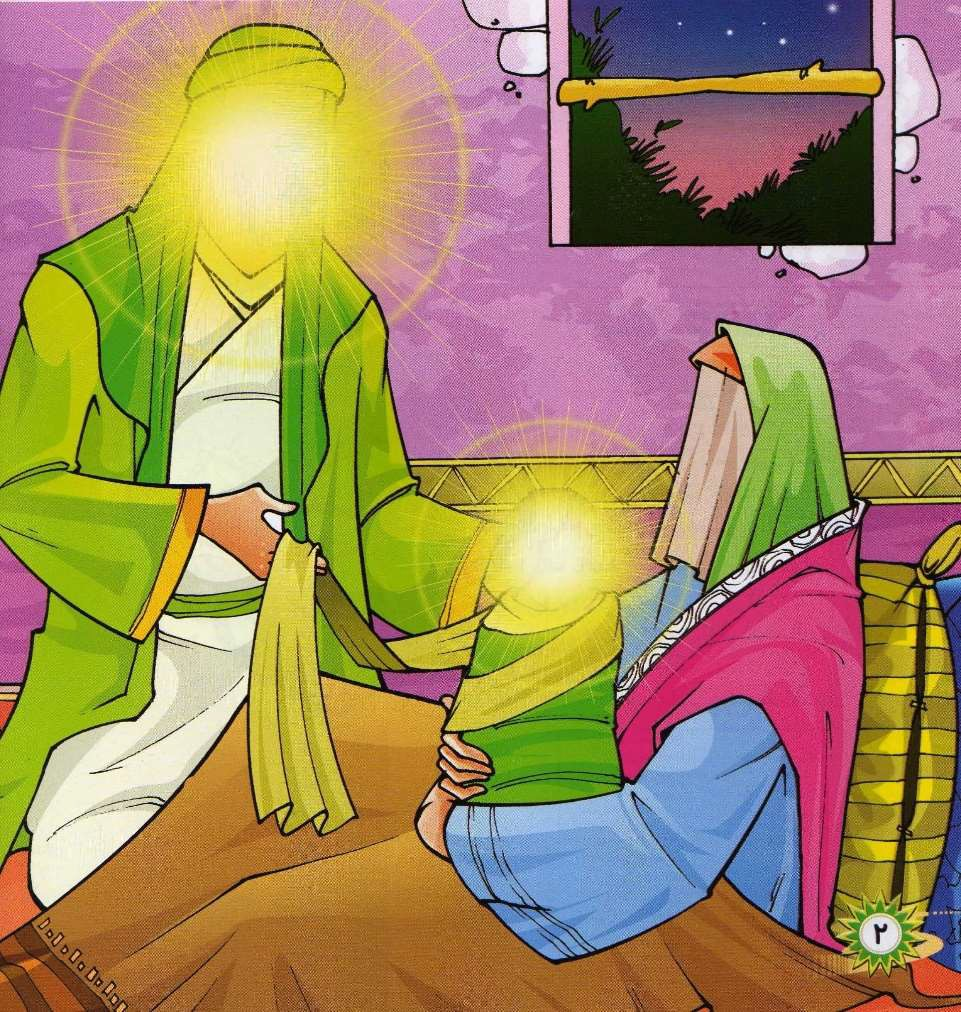
\includegraphics[width=6.3in,height=4.20208in]{media/image4.jpeg}

Selon la théologie musulmane, l'islam est la religion originelle de
l'humanité.VICTOR MOUSSA - STOCK.ADOBE.COM

\subsection{► Que dit la tradition ?}

Selon la théologie musulmane, l'islam est la religion originelle de
l'humanité.~\emph{« Tout homme est né musulman »,}~dit un hadith
attribué
au~\href{https://www.la-croix.com/sacralite-prophete-lislam-2020-11-06-1101123195}{\underline{prophète
Mohammed}}. L'homme est né pour adorer Dieu : certes, il a reçu une
dignité plus haute que les autres créatures, mais celle-ci est
conditionnée à sa soumission au Dieu unique. Plus un homme applique la
loi divine (\emph{charia}), plus il devient humain. Quant au « mécréant
» (\emph{kâfir}), qui refuse de suivre la charia, il se situe en quelque
sorte à un degré inférieur d'humanité.

Cette sévérité envers les non-musulmans s'appuie sur la lecture du texte
coranique qui s'est imposée à partir du IX\textsuperscript{e}~siècle,
lors de la transformation de l'islam en un empire soucieux de se
légitimer. Confortée par des hadiths rédigés à cette époque, elle
dépeint une vérité unique et non négociable. Elle insiste sur les
versets du Coran particulièrement virulents envers les polythéistes,
païens ou idolâtres, qualifiés d'\emph{« associateurs
»}~(\emph{mouchrikoun}) car ils « associent » à Dieu d'autres divinités.

Quant aux athées,~\emph{« ils appartiennent, selon la théologie
musulmane, à une catégorie de mécréance encore inférieure aux
polythéistes, aux juifs et aux chrétiens »,~}explique l'islamologue
Abdessamad Belhaj, chercheur au Centre interdisciplinaire d'études de
l'islam dans le monde contemporain de l'Université catholique de
Louvain. Même si des institutions comme le Haut Conseil des oulémas du
Maroc ou la Maison de la fatwa en Égypte considèrent que les apostats ne
peuvent plus être condamnés à mort, cette peine reste appliquée dans une
dizaine de pays, comme l'Afghanistan ou
la~\href{https://www.la-croix.com/Monde/Afrique/prisons-Mauritanie-calvaire-dun-apostat-2019-09-30-1201051050}{\underline{Mauritanie}}.

\subsection{ Pourquoi juifs et chrétiens bénéficient-ils d'un statut
spécifique ?}

Selon la tradition musulmane, chrétiens et juifs font l'objet d'un
traitement différent des autres non-musulmans : ils bénéficient dans le
droit islamique d'une protection juridique particulière (\emph{dhimma})
toutefois accompagnée d'injonctions humiliantes, comme l'interdiction de
monter à cheval ou de construire des lieux de culte dépassant ceux des
musulmans.
 

\emph{« Le Coran est très ambivalent au sujet des ``gens du Livre''
»,~}rappelle
l'historien~\href{https://www.la-croix.com/Culture/Livres-et-idees/historiens-decryptent-Coran-avant-lislam-2019-11-27-1201063090}{\underline{Guillaume
Dye}}, professeur à l'Université libre de Bruxelles (1). Selon la
sourate 5, juifs et chrétiens ne doivent pas être pris pour~\emph{«
alliés »~}(5, 51) mais, quelques versets plus loin, on lit qu'ils ne
seront~\emph{« point affligés »~}(5, 69). Les chrétiens se voient
reprocher de nier l'unicité de Dieu mais du respect est exprimé pour les
prêtres et les moines, qui~\emph{« ne s'enflent pas d'orgueil ».}

Selon une théologie dite de la falsification (\emph{tahrif}), les juifs
et les chrétiens ont altéré le message transmis par leurs prophètes
respectifs (Moïse, Jésus), message qui n'était autre que l'islam. Le
Coran, lui, corrige cette déviation en transmettant fidèlement le
message révélé à un ultime prophète, Mohammed. À Médine, celui-ci aurait
signé une~\emph{« Constitution »~}disposant que les juifs, notamment,
pouvaient pratiquer leur religion en sécurité, mais ces relations se
sont rapidement détériorées.

\subsection{► Quelles pistes pour une « théologie du pluralisme » ?}

Les attentats visant des « mécréants » en terrasse à Paris, les
persécutions contre les Yézidis ou les chrétiens en Irak, sont autant de
conséquences d'une lecture littéraliste du Coran encouragée par l'essor
du salafisme saoudien à partir des années 1970. D'autres lectures ont
pourtant existé dès les premiers siècles de l'islam. Contrairement à la
doctrine sunnite traditionnelle, l'exégèse rationaliste a par exemple
conclu très tôt à une~\emph{« égalité entre tous les êtres humains, tous
étant dotés de la même raison les rendant aptes à comprendre la parole
de Dieu »,~}rappelle l'islamologue Pierre Lory, directeur d'études à
l'École pratique des hautes études (EPHE).

Pour Abdessamad Belhaj, tout l'enjeu est aujourd'hui de refonder le
rapport à l'altérité sur la base de l'éthique, et de\emph{~« mettre
l'homme au cœur de la théologie »}. Pour cela, certaines valeurs
présentes dans l'islam gagneraient à être redécouvertes, comme celles du
soin, du don et du service à l'humanité, longtemps éclipsées selon lui
par l'autorité et la loyauté à la communauté musulmane ou à la tribu.

(1) Il a codirigé avec Mohammad Ali Amir-Moezzi, Le Coran des
historiens, 2019, Éd. du Cerf, 3~408~p., 89~€.

Faudra-t-il sauver les salafistes ?

Le gouvernement français a voulu lancer en octobre 2019 une offensive
contre l'islamisme et les courants radicaux, rapidement relayée par un
emballement médiatique qui a échappé à tout contrôle. Or, l'ennemi
désigné n'a nullement été identifié selon des termes juridiques, pas
plus que ses torts. On lui reproche sa piété rigoureuse, son voile, sa
pratique du jeûne de Ramadan, sa barbe fournie, son refus de toucher les
femmes, ce qui le rapproche dangereusement de n'importe quel fidèle
conservateur.

L'offensive vise donc une manière de concevoir la piété musulmane, et
nullement une qualification criminelle ou une atteinte à l'ordre public.
C'est dire que nous sommes confrontés à un « délit de sale gueule »,
lequel échappe à la tradition juridique républicaine, délit qui est
indiscernable, sans limite, extensible, mais politiquement pratique
auprès d'une opinion chauffée à blanc par les attentats et
l'immigration.

\subsection{Un engagement d'abord religieux}

Si l'islamiste ainsi décrit ressemble évidemment
au~\href{https://www.la-croix.com/Religion/Islam/Quest-salafisme-2018-10-14-1200975866}{\underline{salafiste}},
c'est oublier un peu vite que l'écrasante majorité des~\emph{salafi~}--
ceux qui sont attachés au modèle des « anciens » (les~\emph{salaf}),
c'est-à-dire les compagnons du Prophète -- se veulent quiétistes : leur
mode d'action est la prédication et l'action missionnaire
(la~\emph{da`wa}). Le salafiste souhaite d'abord vivre un islam épuré et
intégriste -- au sens d'intégral -- dans le cadre de sa famille et de sa
communauté.

Ce mouvement est distinct d'un engagement politique, de sorte que les
salafistes sont rarement liés aux Frères musulmans, qui eux forment un
mouvement politique. Si la matrice religieuse et idéologique du
salafisme imprègne les mentalités djihadistes, elle ne se confond pas
avec celles-ci, ni dans la pensée, ni dans les faits. La radicalisation
concerne donc à des degrés différents et sous des formes incomparables
les sympathisants du salafisme et les partisans du djihadisme de Daech.
Les premiers ont un engagement d'abord religieux, tandis que les autres
sont mus à la fois par la volonté de puissance, des facteurs politiques,
sociaux et religieux.

\subsection{L'autodidacte de l'islam présente plus de risques que le
salafiste}

L'hostilité des salafistes envers les courants djihadistes a été prouvée
à de nombreuses reprises par des déclarations publiques et surtout en
fournissant du renseignement de qualité auprès des services de police.
Le meilleur ennemi du terroriste est souvent le~\emph{salafi}, et
l'autodidacte de l'islam présente plus de risques que le salafiste.

En outre, le salafisme n'a pas été désavoué par les représentants du
culte musulman pour la simple raison que ce courant n'est pas une
idéologie : il faudrait donc lui enlever son~\emph{isme}~final et
l'appeler, selon la tradition religieuse, la~\emph{salafiya~}; il s'agit
d'un vieux courant légitime de l'islam, qui a fourni des générations
d'imams et de lettrés attachés au sens littéral du Coran et de la Sunna.

\subsection{Un « écosystème » étroit mais rassurant}

Il est évident que le salafisme représente une alternative culturelle et
sociale au modèle français, modèle égalitaire, inclusif, ouvert (au
moins en théorie). Les quelques salafi que j'ai connus -- des convertis
à 25 ou 30 \% d'entre eux -- vivaient dans un étroit triangle
géographique. Parce qu'ils souhaitent faire les cinq prières à leur
heure, sans les décaler, et ce dans une salle de prière, ils sont
contraints de vivre et de travailler non loin d'une mosquée. Ils passent
ainsi de leur habitation au lieu de travail et à la salle de prière,
lesquels se situent nécessairement dans un « écosystème » étroit mais
rassurant. Ils ne peuvent guère être exigeants sur le plan
professionnel.

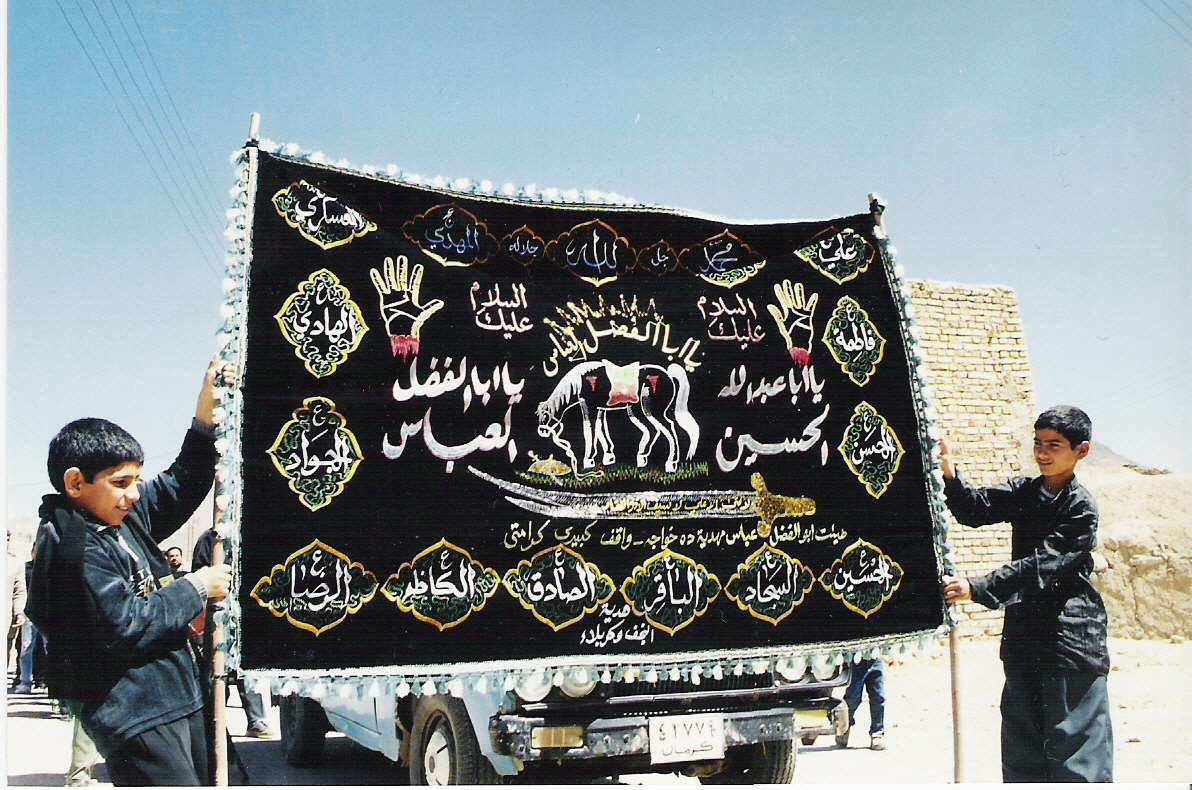
\includegraphics[width=1.97917in,height=1.40972in]{media/image6.jpeg}

\href{https://www.la-croix.com/Religion/Le-Coran-peut-etre-interprete-2021-01-25-1201136852}{Le
Coran peut-il être interprété ?}

Le salafisme, qui représente au moins 40 000 individus, est socialement
dangereux car il impose l'auto-ségrégation, le refus des contacts avec «
ceux qui n'en sont pas ». C'est la raison pour laquelle les spécialistes
des questions de sécurité se refusent à les impliquer dans la lutte
contre le djihadisme. Salafistes et terroristes participeraient à une
même matrice intellectuelle, celle du bien contre le mal, une sorte de
vision sectaire du monde. La différence vient du rapport à la violence :
assumé chez les djihadistes, rejeté chez les salafistes. Leur
fondamentalisme présente l'avantage d'une certaine forme de morale : à
Sartrouville les quartiers salafisés ont vu s'effondrer la toxicomanie
et la délinquance, avec le soutien de la mairie.

\subsection{Confondre l'approche culturelle avec la lutte contre le
terrorisme}

Ces courants ne peuvent être incriminés sur le plan sécuritaire. On
confond donc l'approche culturelle avec la lutte contre le terrorisme. À
moins de changer tout le droit européen, la première doit être menée par
l'éducation, la philosophie, la raison, le débat ; quant à la seconde
elle doit s'appuyer sur le droit et sur des qualifications pénales, et
non sur de vagues impressions de « radicalisation », notion qui n'a
toujours pas été appréhendée de façon rigoureuse en termes sociologiques
et psychologiques.

Comme la guerre d'Algérie nous l'enseigne, une telle manière de
concevoir l'action politique va aboutir à l'effet inverse de celui
recherché : le renforcement de la méfiance collective, le repli
communautaire du côté musulman, l'action violente du côté des « anti »,
et, finalement, la fragmentation sociale et l'insécurité.

\subsection{Islam : les fumées de la radicalisation}

Olivier Hanne, médiéviste (université de Poitiers), chercheur en
islamologie, estime qu'il est très difficile de définir le parcours type
d'une personne radicalisée. Le dernier de trois articles consacrés à
l'islam en France. 
 

Qui parle d'islam aujourd'hui pense aussitôt à la radicalisation. En
2015, on estimait entre 8 000 et 10 000 le nombre de Français
radicalisés. Leurs profils sont si variés qu'il est difficile de donner
des catégories fixes : les mineurs représentent 25 \% des cas, les
femmes 27 \%, les personnes signalées sont plutôt jeunes (entre 16 et 30
ans), leur niveau scolaire est généralement faible, même si l'on
rencontre des diplômés.

La plupart travaillent. Internet représente pour tous ces individus un
passage obligé, même s'il se concrétise différemment : terrain initial
de la radicalisation, facteur de renforcement ou vecteur unique de
l'expression radicale, le partage des contenus djihadistes sur Internet
n'a pas du tout la même fonction chez une adolescente connectée, un
salafiste convaincu et un combattant expérimenté déjà parti en Syrie.

\subsection{Les autorités font feu de tout bois}

De toute évidence, l'attraction pour la radicalité religieuse n'est pas
nécessairement liée à un phénomène de rupture sociale. Les failles de la
société contemporaine (éclatement des familles, déclin des autorités et
des idéologies, chômage, ghettoïsation) créent un terreau facilitateur,
mais nullement déterminant. La frustration individuelle alimente le
recours à des convictions extrêmes, voire le passage à l'acte
terroriste, mais n'est qu'un facteur parmi tant d'autres.

Les autorités font feu de tout bois pour tenter de faire face à une
radicalisation multiforme. En avril 2015, le premier ministre français,
Manuel Valls, annonçait l'ouverture d'une dizaine de centres de
prévention de la radicalisation, dont la plupart furent un échec. Des
sites Internet officiels sont créés et proposent des fiches techniques
contre la radicalisation et le terrorisme, dont le contenu est souvent
simple, voire binaire. Ainsi sur le site
français~\emph{stop-djihadisme.gouv.fr}, un bandeau intitulé «
Radicalisation djihadiste, les premiers signes qui peuvent alerter »
énonce pêle-mêle : « ils se méfient des anciens amis qu'ils considèrent
maintenant comme des impurs » ; « ils changent brutalement leurs
habitudes alimentaires » ; « ils arrêtent d'écouter de la musique car
elle les détourne de leur mission » ; « ils ne regardent plus la
télévision et ne vont plus au cinéma ». Autant de signes extérieurs qui
se rapprochent de l'adolescente anorexique\ldots{} L'efficacité de ces
dispositifs a d'ailleurs été très contestée dès 2015.

\subsection{L'État, tenté d'être omniprésent}

Toute l'entreprise de déradicalisation définit en creux le modèle
positif occidental : monde de loisirs, de consommation, d'épanouissement
personnel et professionnel. Le vocabulaire de la radicalisation masque
le rejet de ce modèle culturel. Et les pouvoirs publics d'hésiter à
appeler leur objectif par son vrai nom : le reconditionnement mental.

Le danger de la déradicalisation se situe dans l'élargissement des
intrusions de l'État : en voulant réinsérer, l'État pénètre dans
l'intimité des individus afin de redéfinir le religieux et lui redonner
une place acceptable. Or, l'État a-t-il compétence pour définir ce
qu'est l'islam, le « bon » islam ? Ne sachant cerner la menace, l'État
est tenté d'être omniprésent, sans en avoir la capacité légale. La
déradicalisation pourrait relever de la posture intellectuelle.

Le problème vient sans doute des hésitations du vocabulaire. Car,
après-tout, qu'est-ce que la radicalisation ? Au
XIX\textsuperscript{e}~le mot anglais~\emph{radical}~était employé pour
désigner les partis politiques britanniques exigeant une réforme
démocratique libérale. Transféré tel quel en France, on l'appliqua aux
partis de gauche, laïques et libéraux qui voulaient réformer la société.

\subsection{Réactions épidermiques}

Le verbe « radicaliser » fut employé régulièrement dans les années
1960-1970 dans une acception politique avec l'idée de « devenir plus
intransigeant, se durcir » ou « plus extrême ». Le premier sens était
donc politique et pas nécessairement négatif. Se déradicaliser était un
synonyme pour « se compromettre ». Appliqué à l'islamisme, le verbe
impose une redéfinition complète des termes : à partir de quand
juge-t-on l'islam intransigeant ou extrême ? par rapport à quelle norme
? à quelle moyenne ?

Les réactions épidermiques qui ont suivi le meurtre de l'enseignant de
Conflans-Sainte-Honorine en octobre 2020 sont tristement révélatrices :
les imams doivent s'exprimer ! les musulmans doivent désavouer le
terrorisme et faire allégeance à la France ! Mais quand ils le font,
c'est encore insuffisant, déloyal et mensonger. Le gouvernement proposa
même qu'ils prient pour la République au cours de la prière collective
du vendredi. Nos références sur la question religieuse restent
tragiquement celles de la Révolution française : comme il y eut les «
prêtres jureurs », adhérant à la loi, contre les « prêtres réfractaires
», obstinés dans leur obéissance à Rome, de la même façon il nous faut
des « imams jureurs », intimement républicains. L'État se retrouve donc
juge des reins et des cœurs.

\bibliography{Theo}
%\bibliographystyle{siam}
%\printbibliography

%\listoftheorems[ignoreall,show={Def}]
%Les courants contemporains de l’islam Glossaire général

\mn{Vérifier les termes}

bid‘a : innovation ; pratique « déviante ».

da‘wa : invitation ; prédication – appel à la conversion (dans les deux sens).

fasiq : pécheur ; mauvais musulman.

fiqh : compréhension ; corpus du droit musulman.

fitna: discorde, querelle ; conflit interne au monde musulman.

hadith : récit d’un dire ou faire du Prophète, rapporté par ses compagnons.

hajj : pèlerinage annuel à La Mecque.

hijra (héjire) : « exode » - départ de Mahomet pour Médine (622).

‘ibadat : culte ; partie du droit traitant du culte.

ijma‘ : consensus ; consensus des ulama sur un point de droit.

ijtihad : effort ; effort d’interprétation du Coran.

imam : chef suprême de la communauté musulmane ; successeur du Prophète, utilisé communément par les chiites pour Ali et ses descendants.

islah : réforme.

isnad : chaîne ; chaîne de transmission des hadiths.

jihad : lutte ; soit intérieure, contre ses propres faiblesses ; soit extérieure, contre les ennemis de la communauté musulmane.

ka‘aba : monument cubique noir situé au centre de la grande mosquée de La Mecque ; selon les musulmans, désigne l’emplacement du premier autel élevé par Abraham pour le Dieu unique. Point vers lequel se dirigent les musulmans pour prier.

kafir : infidèle, mécréant

khalifa (calife) : successeur, représentant ; successeur du Prophète et chef de la communauté musulmane (sunnisme).

madrasa : école ; lieu où est assuré la transmission du savoir religieux.

mihrab : niche indiquant la direction de La Mecque dans une mosquée.
 
mu‘amalat : relations ; partie du droit traitant des relations humaines.

qibla : orientation de la prière rituelle (salat), correspondant à la direction de La Mecque.

qiyas : raisonnement par analogie (domaine du droit)

salat : prière rituelle.

seyyed : prince, chef ; descendant du Prophète par Hossein ou Hassan, fils d’Ali.

shari‘a : sentier, voie ; loi divine.

sheykh (cheykh) : vieil homme ; chef d’une tribu ; chef religieux ; personne à la tête d’une congrégation soufie, ayant la capacité de guider ses disciples.

shirk : associationnisme : fait d’adorer d’autres êtres en dehors de Dieu.

shura : principe de consultation soufi : mystique musulman sourate : chapitre du Coran
sunna : coutume ; pratiques du Prophète et de la première communauté musulmane, faisant autorité pour guider le mode de vie des croyants et déterminer la loi religieuse.

tafsir : commentaire du Coran.

tajdid : renouveau (=>mujaddidi : qui renouvelle)

taqlid : imitation ; imitation stérile des anciens (par opposition à l’ijtihad).

tariqa : voie : confrérie soufie.

tawhid : unicité (divine). Dogme fondamental de l’islam.

ulama (oulémas) : terme collectif pour désigner les lettrés musulmans.

umma : peuple ou communauté ; communauté islamique dans son ensemble.

waqf : bien immobilier ou foncier dit « de-main-morte », dépendant des institutions religieuses.

zakat : aumône rituelle, obligatoire pour les croyants.

%\listoftheorems


\end{document}